% !TeX spellcheck = en_US
% !BIB program = biber 
\documentclass{article}

%% Encoding
\usepackage[T1]{fontenc}
\usepackage[utf8]{inputenc}

%% Fonts
% Math fonts (fourier) with utopia (erewhon) text fonts
\usepackage{fourier, erewhon}

%% Setup
% This package contains logos
\usepackage[autoload]{adn}

\setlogos[
\textbf{MO435 --- Probabilistic Machine Learning}\\%[5pt]
\uppercase{Instituto de Computação --- UNICAMP}\\%[-7pt]
]%
{IC3D}%
{UNICAMP}

%% Transform section references
\makeatletter
\renewcommand*{\p@section}{\S\,}
\renewcommand*{\p@subsection}{\S\,}
\makeatother

%% Shorthands
\usepackage{xspace}
\makeatletter
\DeclareRobustCommand\onedot{\futurelet\@let@token\@onedot}
\def\@onedot{\ifx\@let@token.\else.\null\fi\xspace}

\def\eg{e.g\onedot} \def\Eg{E.g\onedot}
\def\ie{i.e\onedot} \def\Ie{I.e\onedot}
\def\cf{cf\onedot} \def\Cf{Cf\onedot}
\def\etc{etc\onedot} \def\vs{vs\onedot}
\def\wrt{w.r.t\onedot} \def\dof{d.o.f\onedot}
\def\etal{et al\onedot}
\makeatother

%%%
% Other packages start here (see the examples below)
%%

%% Figues
\usepackage{graphicx}
\graphicspath{{../output/}}
\usepackage{caption}
\usepackage{subcaption}
\usepackage{array}
\usepackage{multirow}

%% References
% Use this section to embed your bibliography
% Instead of having a separate file, just place the bibtex entries here
\usepackage{filecontents}% create files
\begin{filecontents}{\jobname.bib}
  @article{sathya2013,
    doi = {10.14569/ijarai.2013.020206},
    year = {2013},
    publisher = {The Science and Information Organization},
    volume = {2},
    number = {2},
    author = {R. Sathya and Annamma Abraham},
    title = {Comparison of Supervised and Unsupervised Learning Algorithms for Pattern Classification},
    journal = {International Journal of Advanced Research in Artificial Intelligence}
  }
  @book{bishop2006,
    author = {Bishop, Christopher M.},
    edition = 1,
    isbn = {0-387-31073-8},
    publisher = {Springer},
    title = {Pattern Recognition and Machine Learning},
    year = 2006
  }
  @book{murphy2012,
  title={Machine Learning: A Probabilistic Perspective},
  author={Murphy, Kevin P},
  pages={27--33},
  year={2012},
  publisher={The MIT Press},
  }
\end{filecontents}
% Include bibliography file
\usepackage[
backend=biber, 
style=ieee, 
natbib=true,
]{biblatex}
\addbibresource{\jobname.bib}

%% Math
\usepackage{amsmath}

%% Enumerate
\usepackage{enumitem}

\begin{document}

% Put the topic of the assignment here
\title{Project 1}
% Put your name here 
\author{
Jo\~ao Victor da Silva Guerra 
and
Leonardo Alves de Melo
\thanks{117410 and 156188. j117410@dac.unicamp.br and leonardo.alves.melo.1995@gmail.com.}
}

\maketitle

\begin{abstract}
  In this project, we implemented two approaches of machine learning classifiers: generative and discriminative. For the generative model, we created two datasets with three classes and evaluated the performance of our model based on them. We also described the model derivation to obtain our model. On the other hand, for the discriminative model, we created one dataset with two classes and evaluated the performance of our model based on them. Further, we evaluated the effects of the learning rate in the gradient descent algorithm and the sample size in the Monte Carlo approximation. Finally, we sucessfully implemented both models with good performance metrics, such as accuracy, precision and recall.
\end{abstract}

\section{Introduction}

Classification plays an essential role in the field of Machine Learning techniques.
The main goal is to predict classes ($y$) of a set of data points ($x$), modelled by a mapping function ($f(x)$). A powerful approach to tackle classification problems are to model the conditional probability distribution ($p(y = C_{i}|x)$) in an inference stage and use it to classify new data across a set of classes ($y = \{C_{1}, ..., C_{n}$\}). When classes have already been assigned to the input data, the classification belongs to the category of supervised learning. In this scenario, a sample of data from the input data is used for adjusting the parameters of the classifier model \cite{bishop2006, murphy2012, sathya2013}.

There are two approaches to determine the conditional probability distribution, a generative and a discriminative. The first approach models the class-conditional density $(p(x|C_{i}))$ and the class prior ($p(C_{i})$), which applies the Bayes' theorem to model the conditional probability, as described in Eq.\eqref{eq1}. The latter approach models the conditional probability distribution directly, optimizing a parametric model, as described in Eq.\eqref{eq2}. Both approaches adjust their model's parameters from training data.

\begin{equation}
  \label{eq1}
  p(C_{i}|x) = \dfrac{p(x,C_{i})}{p(x)} = \dfrac{p(x|C_{i})p(C_{i})}
  {\sum_{j} p(x|C_{j})p(C_{j})}
\end{equation}

\begin{equation}
  \label{eq2}
  p(C_{i}|x, W) = \dfrac{\exp(w_{i}^{T}x)}{\sum_{j} \exp(w_{j}^{T}x)}
\end{equation}

\section{Probabilistic generative model}

\subsection{Data}

For our experiments, we created two datasets composed by 150 data points divided equally in three classes, named as A and B (Fig. \ref{fig:data}). 
Each data point has two features (Feature 1 and Feature 2). In addition, we split each dataset in two partitions of 75 data points, i. e. training set and test set, with each class equally distributed.

\begin{figure}
  \centering
  \begin{subfigure}[t]{0.49\textwidth}
    \centering
    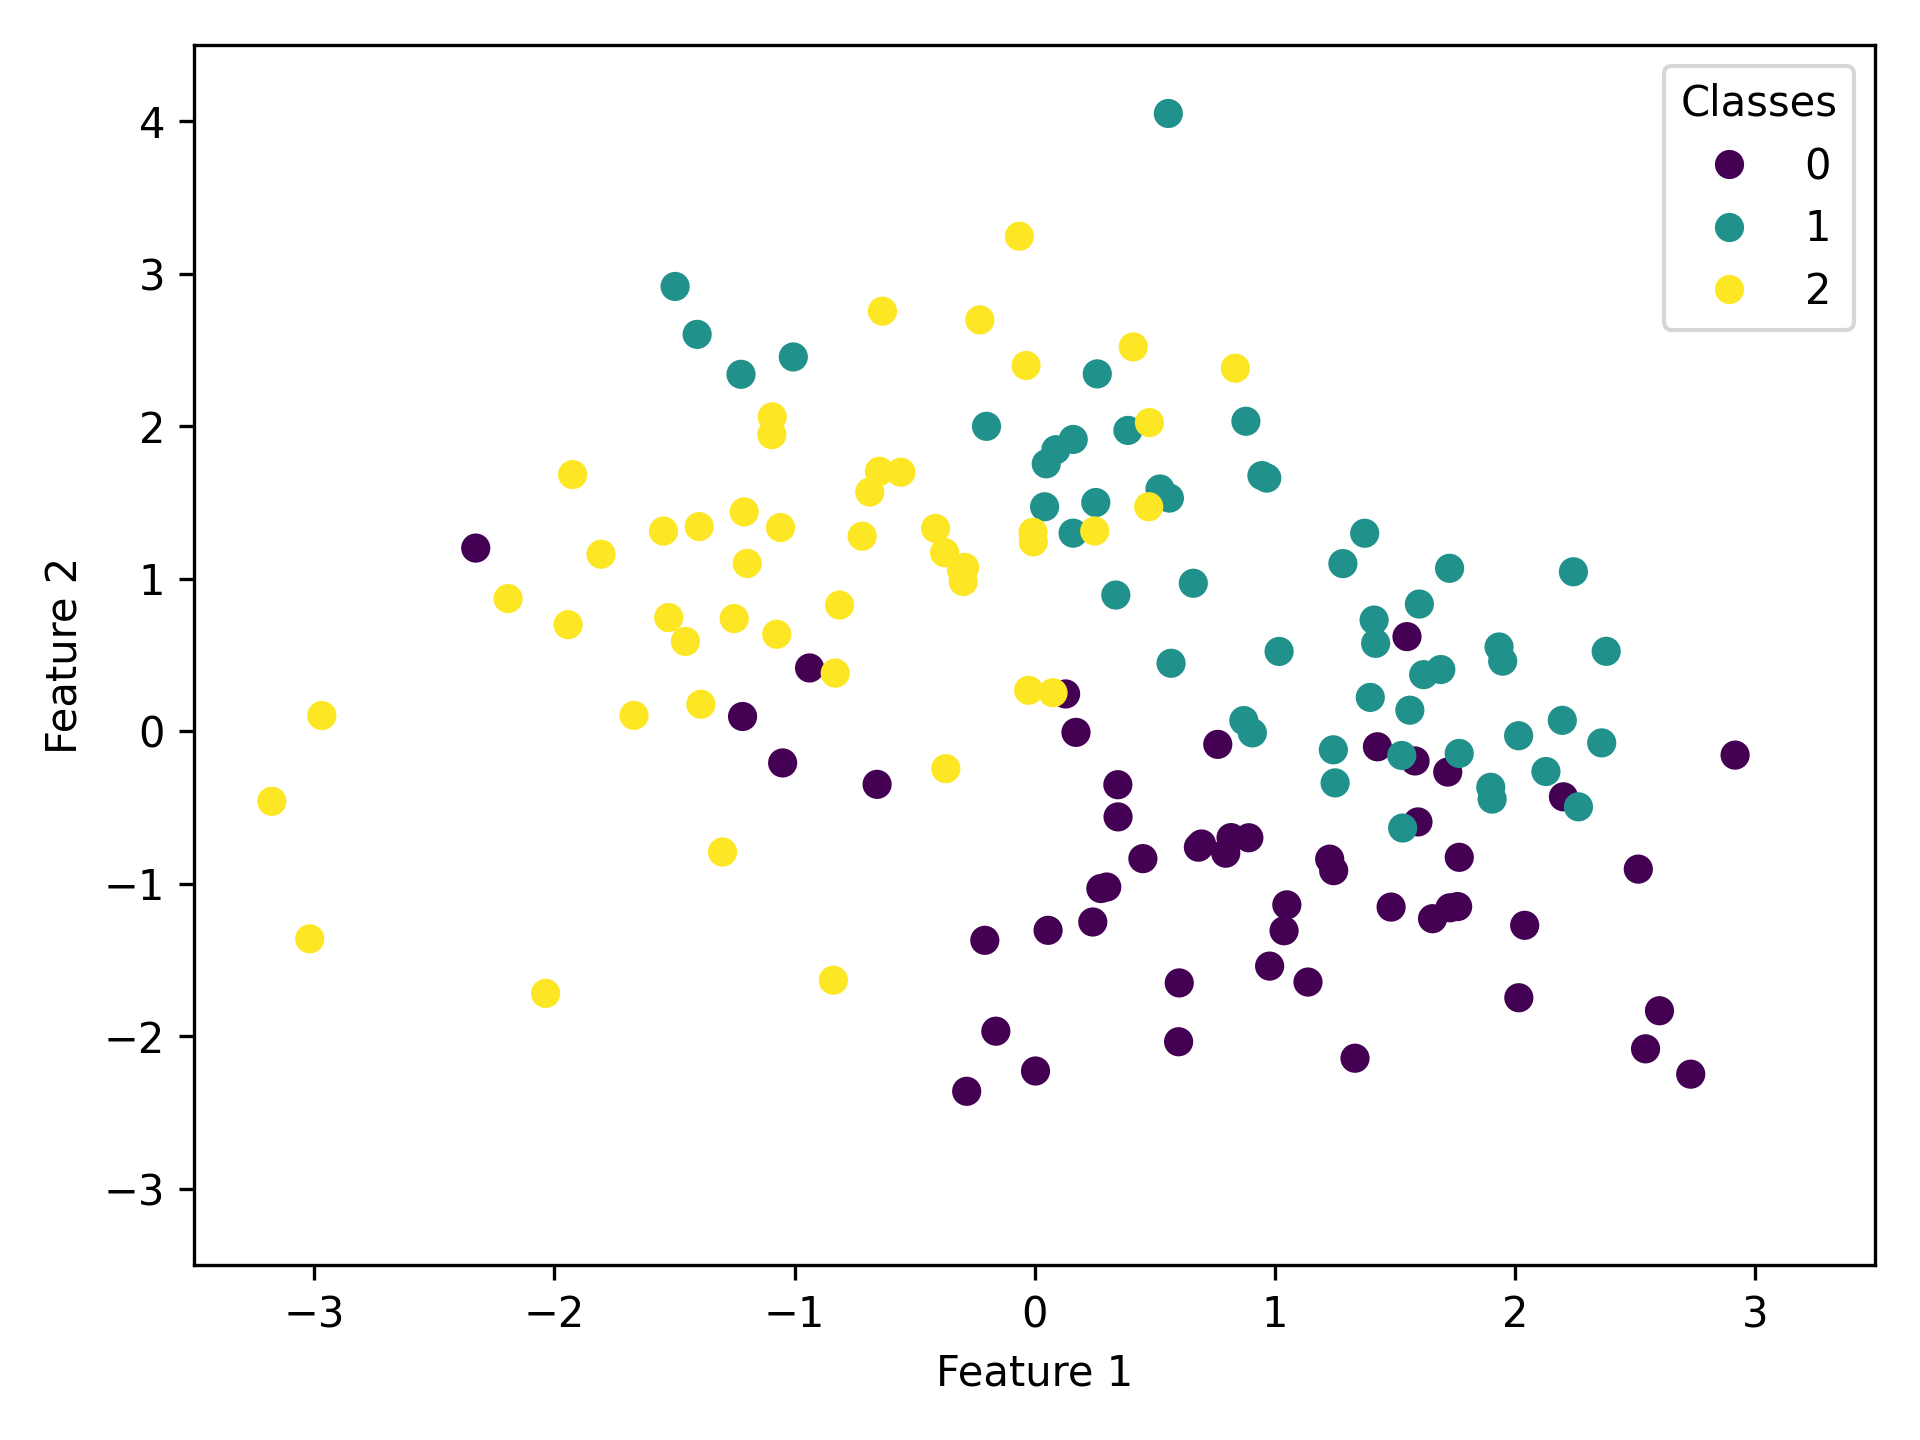
\includegraphics[width=\linewidth]{scatter_A.png}
    \caption{Dataset A}
  \end{subfigure}
  \hfill
  \begin{subfigure}[t]{0.49\textwidth}
    \centering
    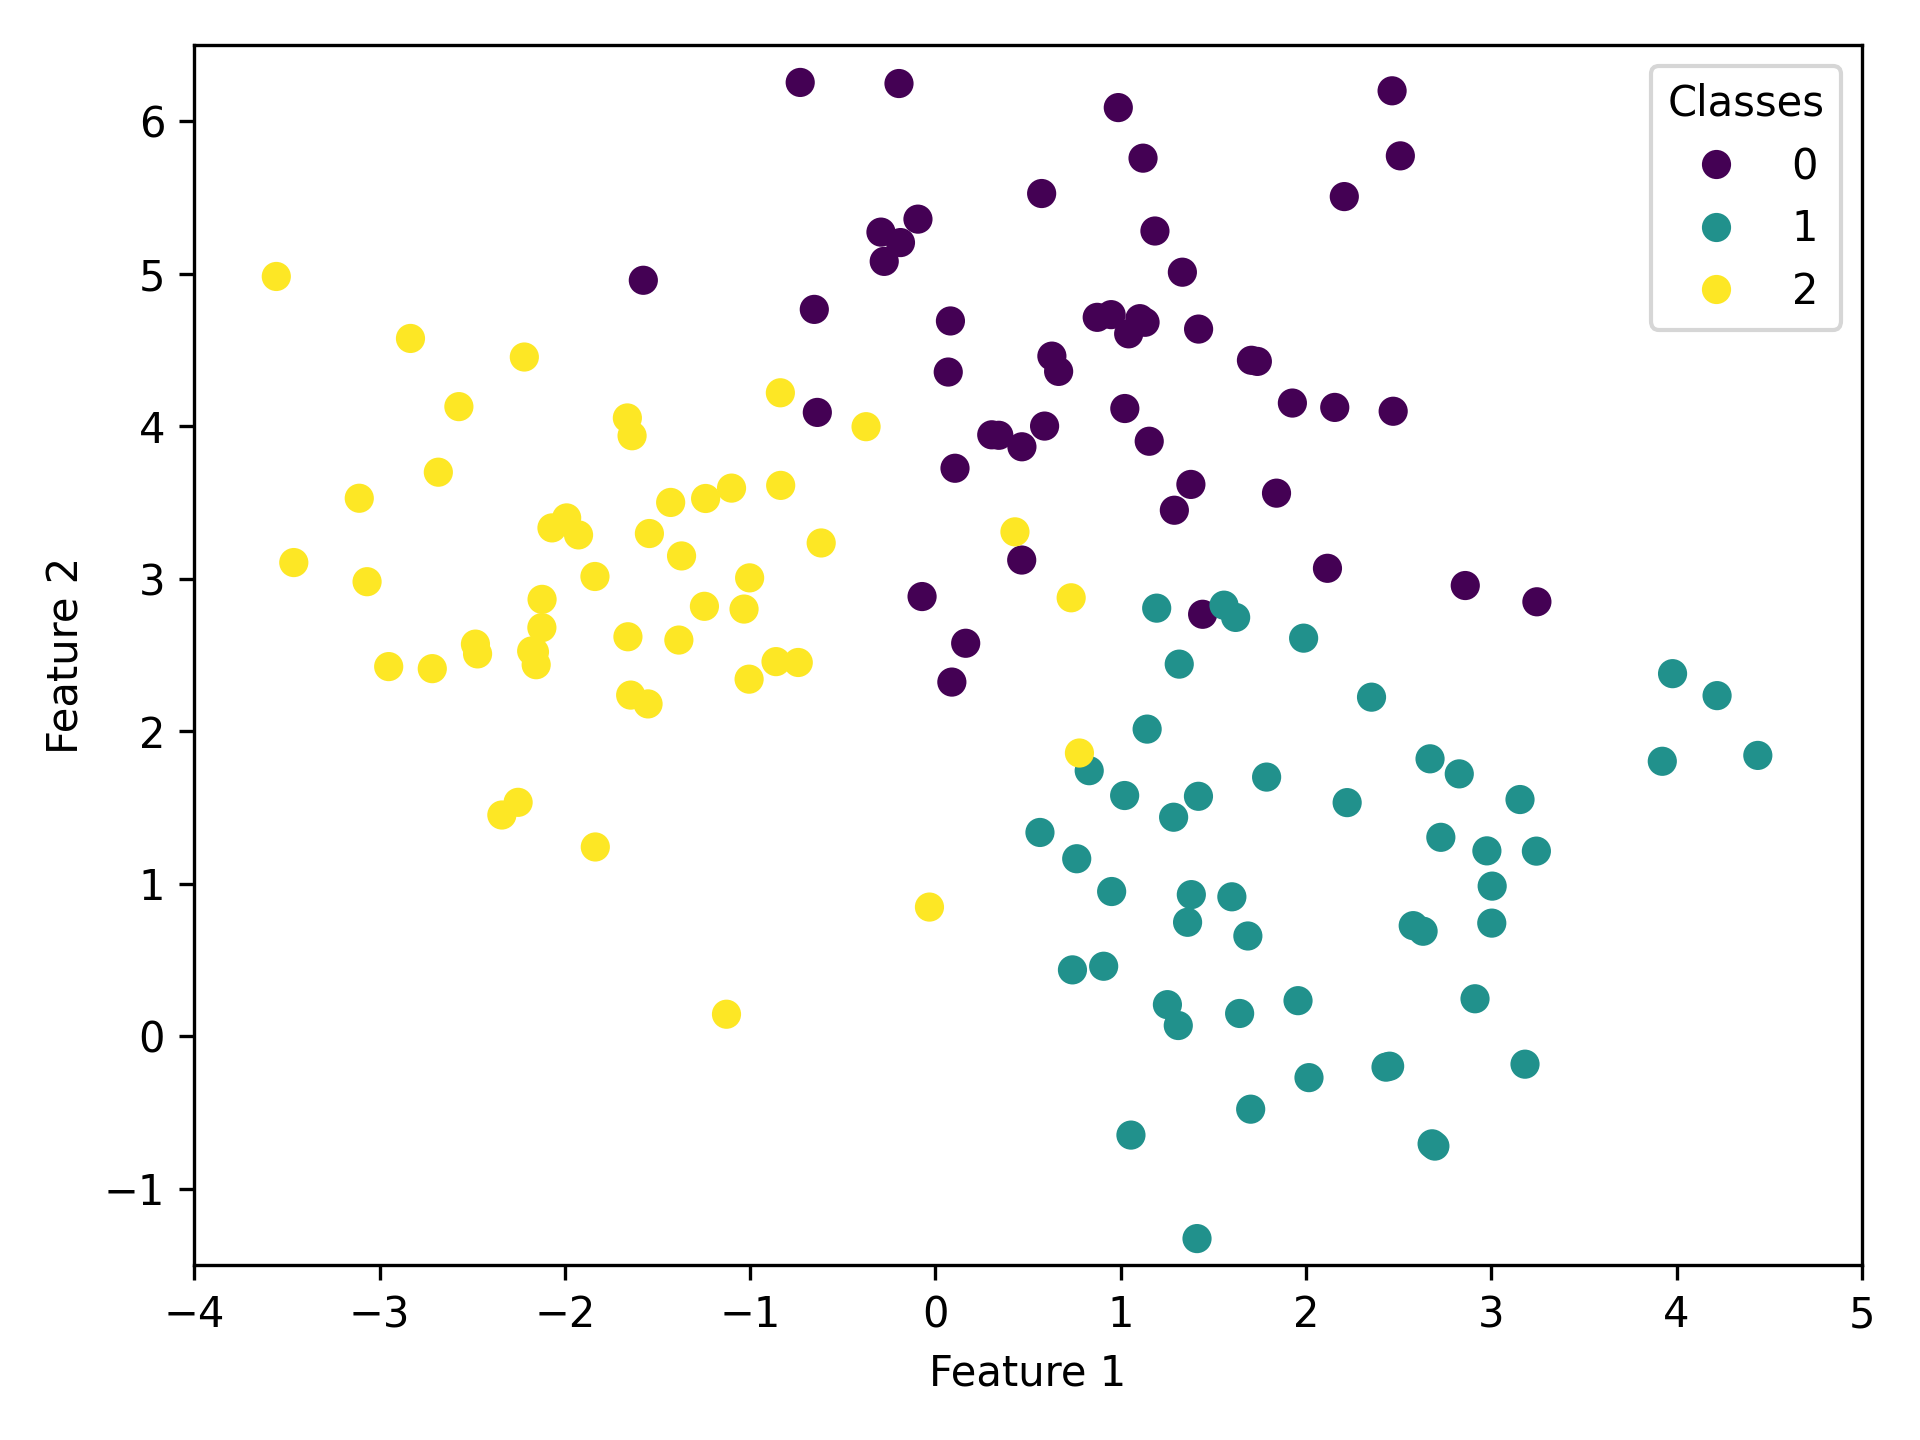
\includegraphics[width=\linewidth]{scatter_B.png}
    \caption{Dataset B}
  \end{subfigure}
  \caption{Scatter plot of datasets by class}
  \label{fig:data}
\end{figure}

\subsection{Model}

Here, we shall derive Eq.\eqref{eq1} for our three-class classification problem. First of all, a parametric form must be adopted for the class-conditional densities, then we assume a Gaussian distribution ($\mathcal{N}$) with shared covariance matrix ($\Sigma$), as described in Eq.\eqref{eq3}.

\begin{equation}
  \label{eq3}
  p(x|C_{i}) \sim \mathcal{N}(x|\mu_{i},\Sigma) = 
  \dfrac{1}{\sqrt{(2\pi)^{(D/2)}|\Sigma|}}
  \exp\left\{-\dfrac{1}{2}(x-\mu_k)^{T}\Sigma^{-1}(x-\mu_k)\right\}
\end{equation}
where $\mu_{i}$ is the mean vector and $D$ is the number of features.

Once we assumed a parametric form for the class-conditional density, we shall determine its parameters ($\mu_i$, $\Sigma$) and the class prior ($p(C_i)$), using the maximum likelihood solution. 
Consider our training set $\{x_n, t_n\}$, where $n = [0,75)$, $t_n = 0$ denotes class $C_0$, $t_n = 1$ denotes class $C_1$ and $t_n = 2$ denotes class $C_2$. The class prior is given by $p(C_i) = \pi_i$. Hence, the likelihood function is

\begin{equation}
\label{eq4}
p({x_n, t_n}| {\pi_i}) = \prod_{n=0}^{74} \prod_{i=0}^{2} \left\{\mathcal{N}(x_n|\mu_{i},\Sigma)\pi_i\right\}^{t_{ni}}
\end{equation}
and applying the logarithm, we get the log-likelihood function as

\begin{equation}
\label{eq5}
\ln{p({x_n, t_n}| {\pi_i})} = \sum_{n=0}^{74} \sum_{i=0}^{2} t_{ni} \left\{ \ln{\mathcal{N}(x_n|\mu_{i},\Sigma)} + \ln{\pi_i} \right\}.
\end{equation}

\subsubsection{Prior class probability}

We shall maximize the log-likelihood with respect to $\pi_i$ but ensuring the constraint $\sum_i \pi_i = 1$. For this, we introduce a Lagrange multiplier $\lambda$ in Eq.\eqref{eq5} as 

\begin{equation}
\label{eq6}
\ln{p({x_n, t_n}| {\pi_i})} + \lambda \left(\sum_{i=0}^2 \pi_i = 1\right)
\end{equation}
and differentiate in relation to $\pi_i$ and set the result to zero, yields

\begin{equation}
  \label{eq7}
  \sum_{n=0}^{74} \dfrac{t_{ni}}{\pi_i} + \lambda = \dfrac{N_i}{\pi_i} + \lambda = 0.
\end{equation}

Summing Eq.\eqref{eq7} over the three classes, we obtaing that $\lambda=-N$, and using this in Eq.\eqref{eq7}, we obtain

\begin{equation}
  \label{eq8}
  \pi_i = \dfrac{N_i}{N}.
\end{equation}

\subsubsection{Class-conditional densities}
Now we must consider the Gaussian distribution (Eq.\eqref{eq3}) in the log-likelihood function as

\begin{equation}
\label{eq9}
\ln{p({x_n, t_n}| {\pi_i})} = -\dfrac{1}{2} \sum_{n=0}^{74} \sum_{i=0}^{2} t_{ni} \left[ \ln{|\Sigma|} + (x_n - \mu_i)^T\Sigma^{-1}(x_n - \mu_i) + \ln{\pi_i} \right]
\end{equation}
where $\ln{\pi_i}$ is constant and independent of $\mu_i$ and $\Sigma$.

Hence, we shall maximize the log-likelihood with respect to $\mu_i$, setting the derivate in relation to $\mu_i$ to zero, we obtain

\begin{equation}
\label{eq10}
\sum_{n=0}^{74} t_{ni} (x_n - \mu_i) = 0 \implies \mu_i = \dfrac{1}{N_i} \sum_{n=0}^{74} t_{ni} x_n
\end{equation}

Finally, we shall maximize the log-likelihood with respect to $\Sigma$. Choosing the terms dependent on $\Sigma$, we can rearrange it as

\begin{equation*}
-\dfrac{N}{2}\ln{|\Sigma|} - \dfrac{1}{2} \sum_{n=0}^{74} \sum_{i=0}^{2} t_{ni}  \left[(x_n - \mu_i)^T\Sigma^{-1}(x_n - \mu_i)\right]
\end{equation*}

\begin{equation*}
= -\dfrac{N}{2}\ln{|\Sigma|} - \dfrac{N}{2} tr\left( \Sigma^{-1} \dfrac{1}{N} \sum_{n=0}^{74} \sum_{i=0}^{2} t_{ni}  \left[(x_n - \mu_i)(x_n - \mu_i)^T\right]\right)
\end{equation*}

\begin{equation}
\label{eq11}
= -\dfrac{N}{2}\ln{|\Sigma|} - \dfrac{N}{2} tr\left(\Sigma^{-1}S\right).
\end{equation}
where we define

\begin{equation}
\label{eq12}
S = \sum_{i=0}^{2} \dfrac{N_i}{N} S_i
\end{equation}

\begin{equation}
\label{eq13}
S_i = \dfrac{1}{N_i} \sum_{n=0}^{74} t_{ni} \left[(x_n - \mu_i)(x_n - \mu_i)^T\right]
\end{equation}

Then, differentiating Eq.\eqref{eq11} in relation to $\Sigma$ and equating to zero, we obtain that $\Sigma = S$.

\subsubsection{Results}

With our training sets, we adjusted the parameters $\mu_i$, $\Sigma$ and prior probabilities ($\pi_i$) for datasets A and B, which are shown in Table \ref{tab:1}. Then, we replace the parameters in the Eq.\eqref{eq1}, and obtained the following expression for the conditional probability of each class for each data point

\begin{equation}
  \label{eq14}
  p(C_i|x) = \dfrac{\mathcal{N}(x|\mu_{i},\Sigma) \pi_i}{\mathcal{N}(x|\mu_{0},\Sigma) \pi_0 + \mathcal{N}(x|\mu_{1},\Sigma) \pi_1 + \mathcal{N}(x|\mu_{2},\Sigma) \pi_2}.
\end{equation}

\begin{table}[h]
  \centering
  \caption{Parameters adjusted through maximum likelihood solution for datasets A and B.} \label{tab:1}
  \begin{tabular}{ccccccccc}
  \hline
  \textbf{Dataset} & \textbf{$\pi_0$} & \textbf{$\pi_1$} & \textbf{$\pi_2$} & \textbf{$\mu_0$} & \textbf{$\mu_1$} & \textbf{$\mu_2$} & \textbf{$\Sigma$} \\ \hline
  \textbf{A} & $\dfrac{1}{3}$ & $\dfrac{1}{3}$ & $\dfrac{1}{3}$ & $\left[\begin{array}{c} 0.76 \\ -0.93\end{array}\right]$ & $\left[\begin{array}{c} 0.86 \\ 0.99\end{array}\right]$ & $\left[\begin{array}{c} -1.03 \\ 0.93\end{array}\right]$ & $\left[\begin{array}{cc} 1.20 & -0.23\\ -0.23 & 0.85\end{array}\right]$ \\
  \textbf{B} & $\dfrac{1}{3}$ & $\dfrac{1}{3}$ & $\dfrac{1}{3}$ & $\left[\begin{array}{c} 0.83 \\ 4.45\end{array}\right]$ & $\left[\begin{array}{c} 2.03 \\ 1.19\end{array}\right]$ & $\left[\begin{array}{c} -1.70 \\ 3.00\end{array}\right]$ & $\left[\begin{array}{cc} 1.24 & -0.24\\ -0.24 & 1.05\end{array}\right]$  \\ \hline
 \end{tabular}
\end{table}

Given any data point $x$, we calculate the conditional probability for the classes 0, 1 and 2. Hence, the data point is predicted to the class with the higher conditional probability, as described in Eq.\eqref{eq15}.

\begin{equation}
  \label{eq15}
  \hat{C} = \underset{C_i}{\mathrm{argmax}}\:p(C_i|x)
\end{equation}

Finally, we ploted a scatter plot with all data points (training and test set) colored by the actual class and the background colored by the predicted class with the linear decision boundaries (Fig. \ref{fig:pred}).  

\begin{figure}[h]
  \centering
  \begin{subfigure}[t]{0.49\textwidth}
    \centering
    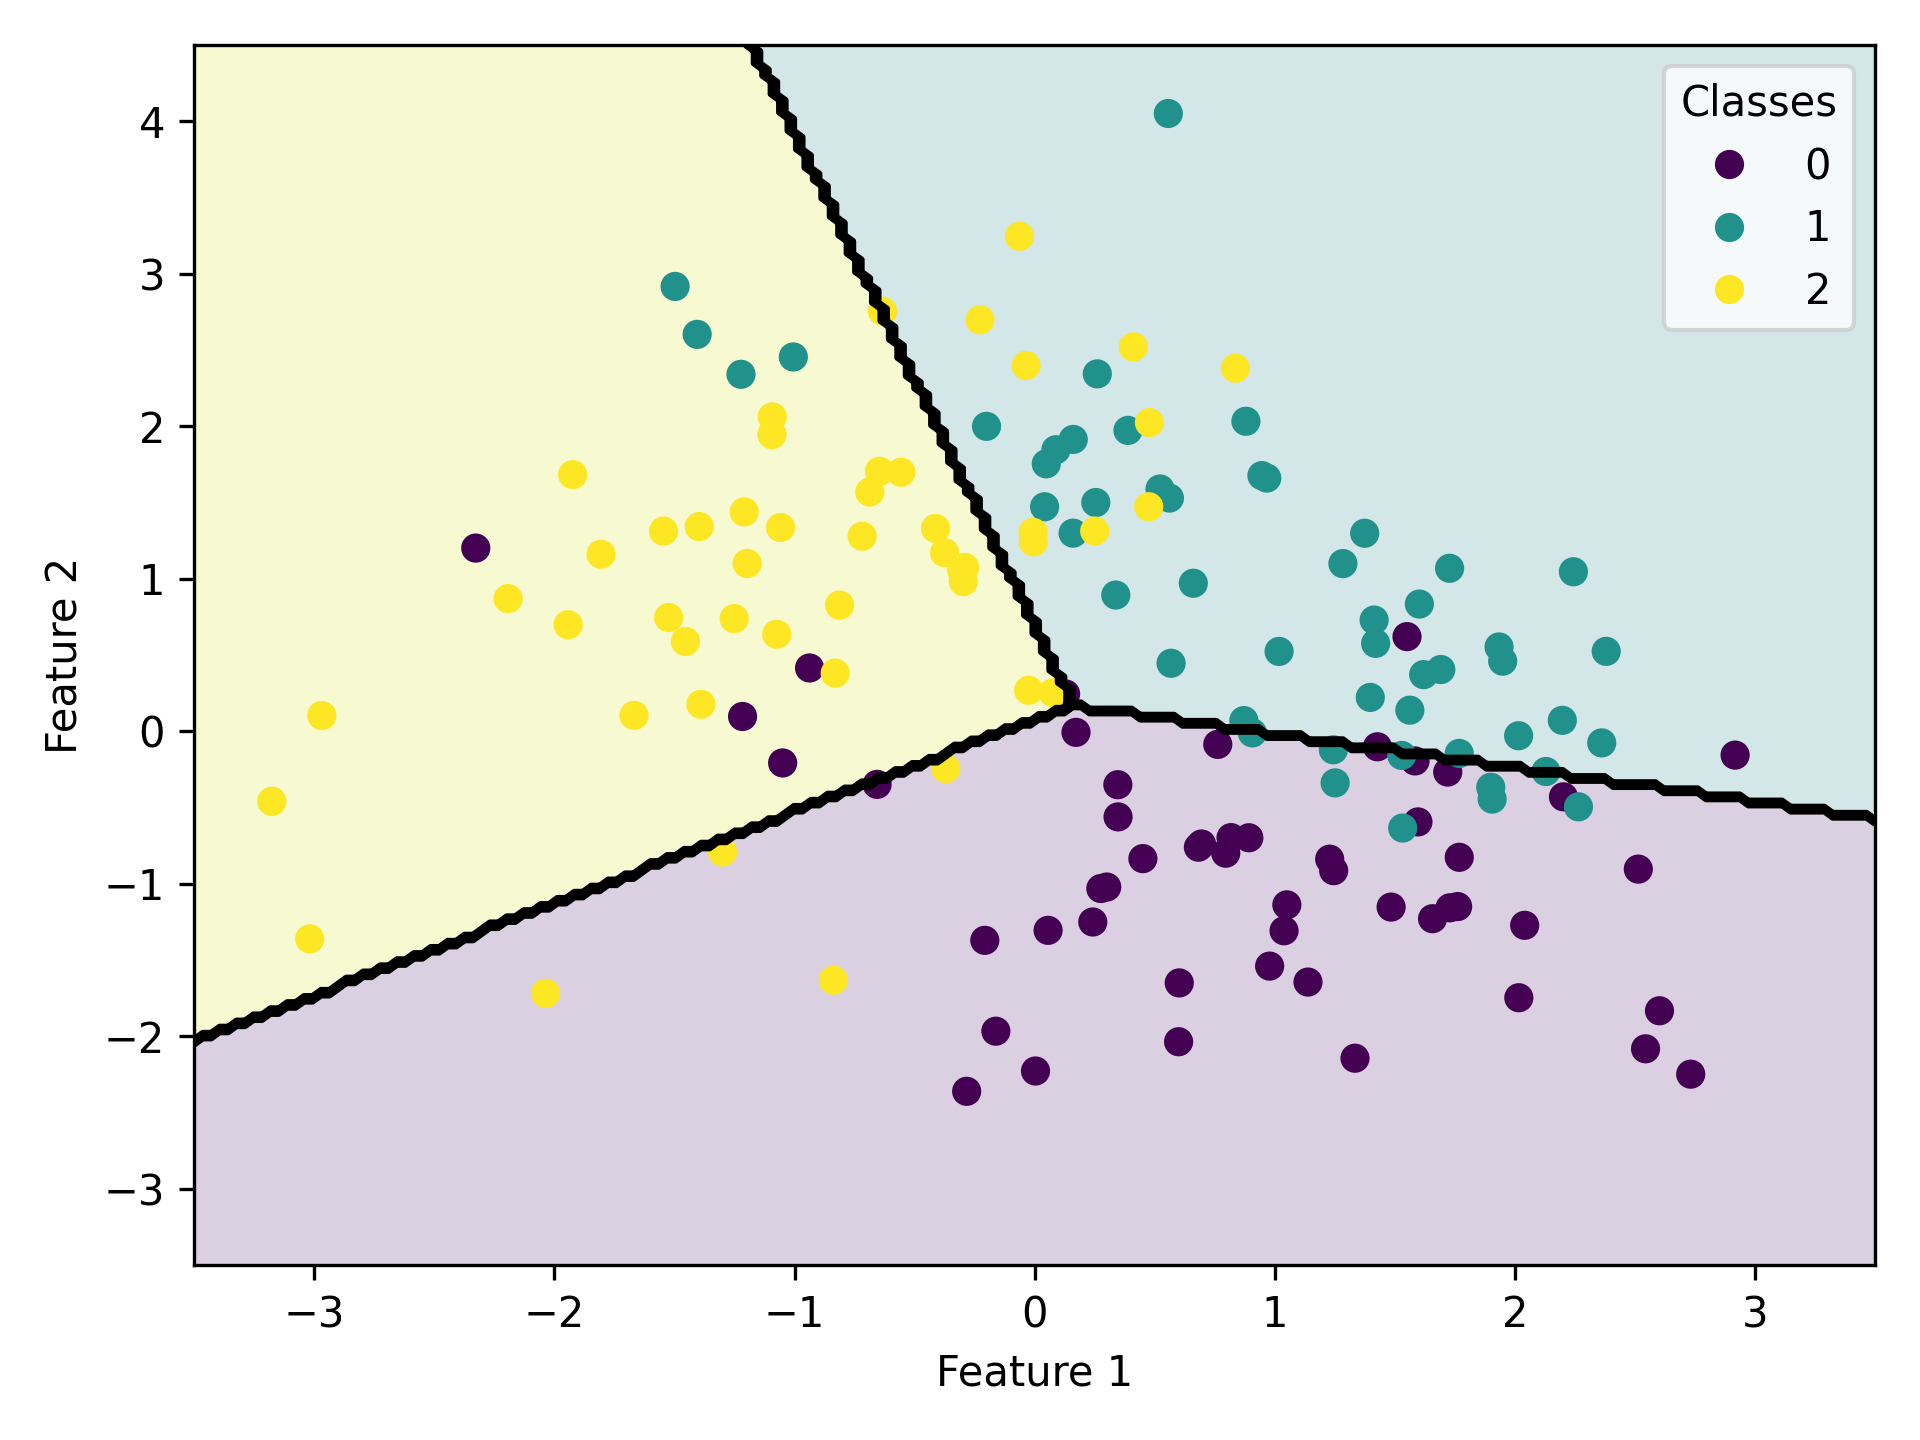
\includegraphics[width=\linewidth]{scatter_with_contour_A.png}
    \caption{Dataset A}
  \end{subfigure}
  \hfill
  \begin{subfigure}[t]{0.49\textwidth}
    \centering
    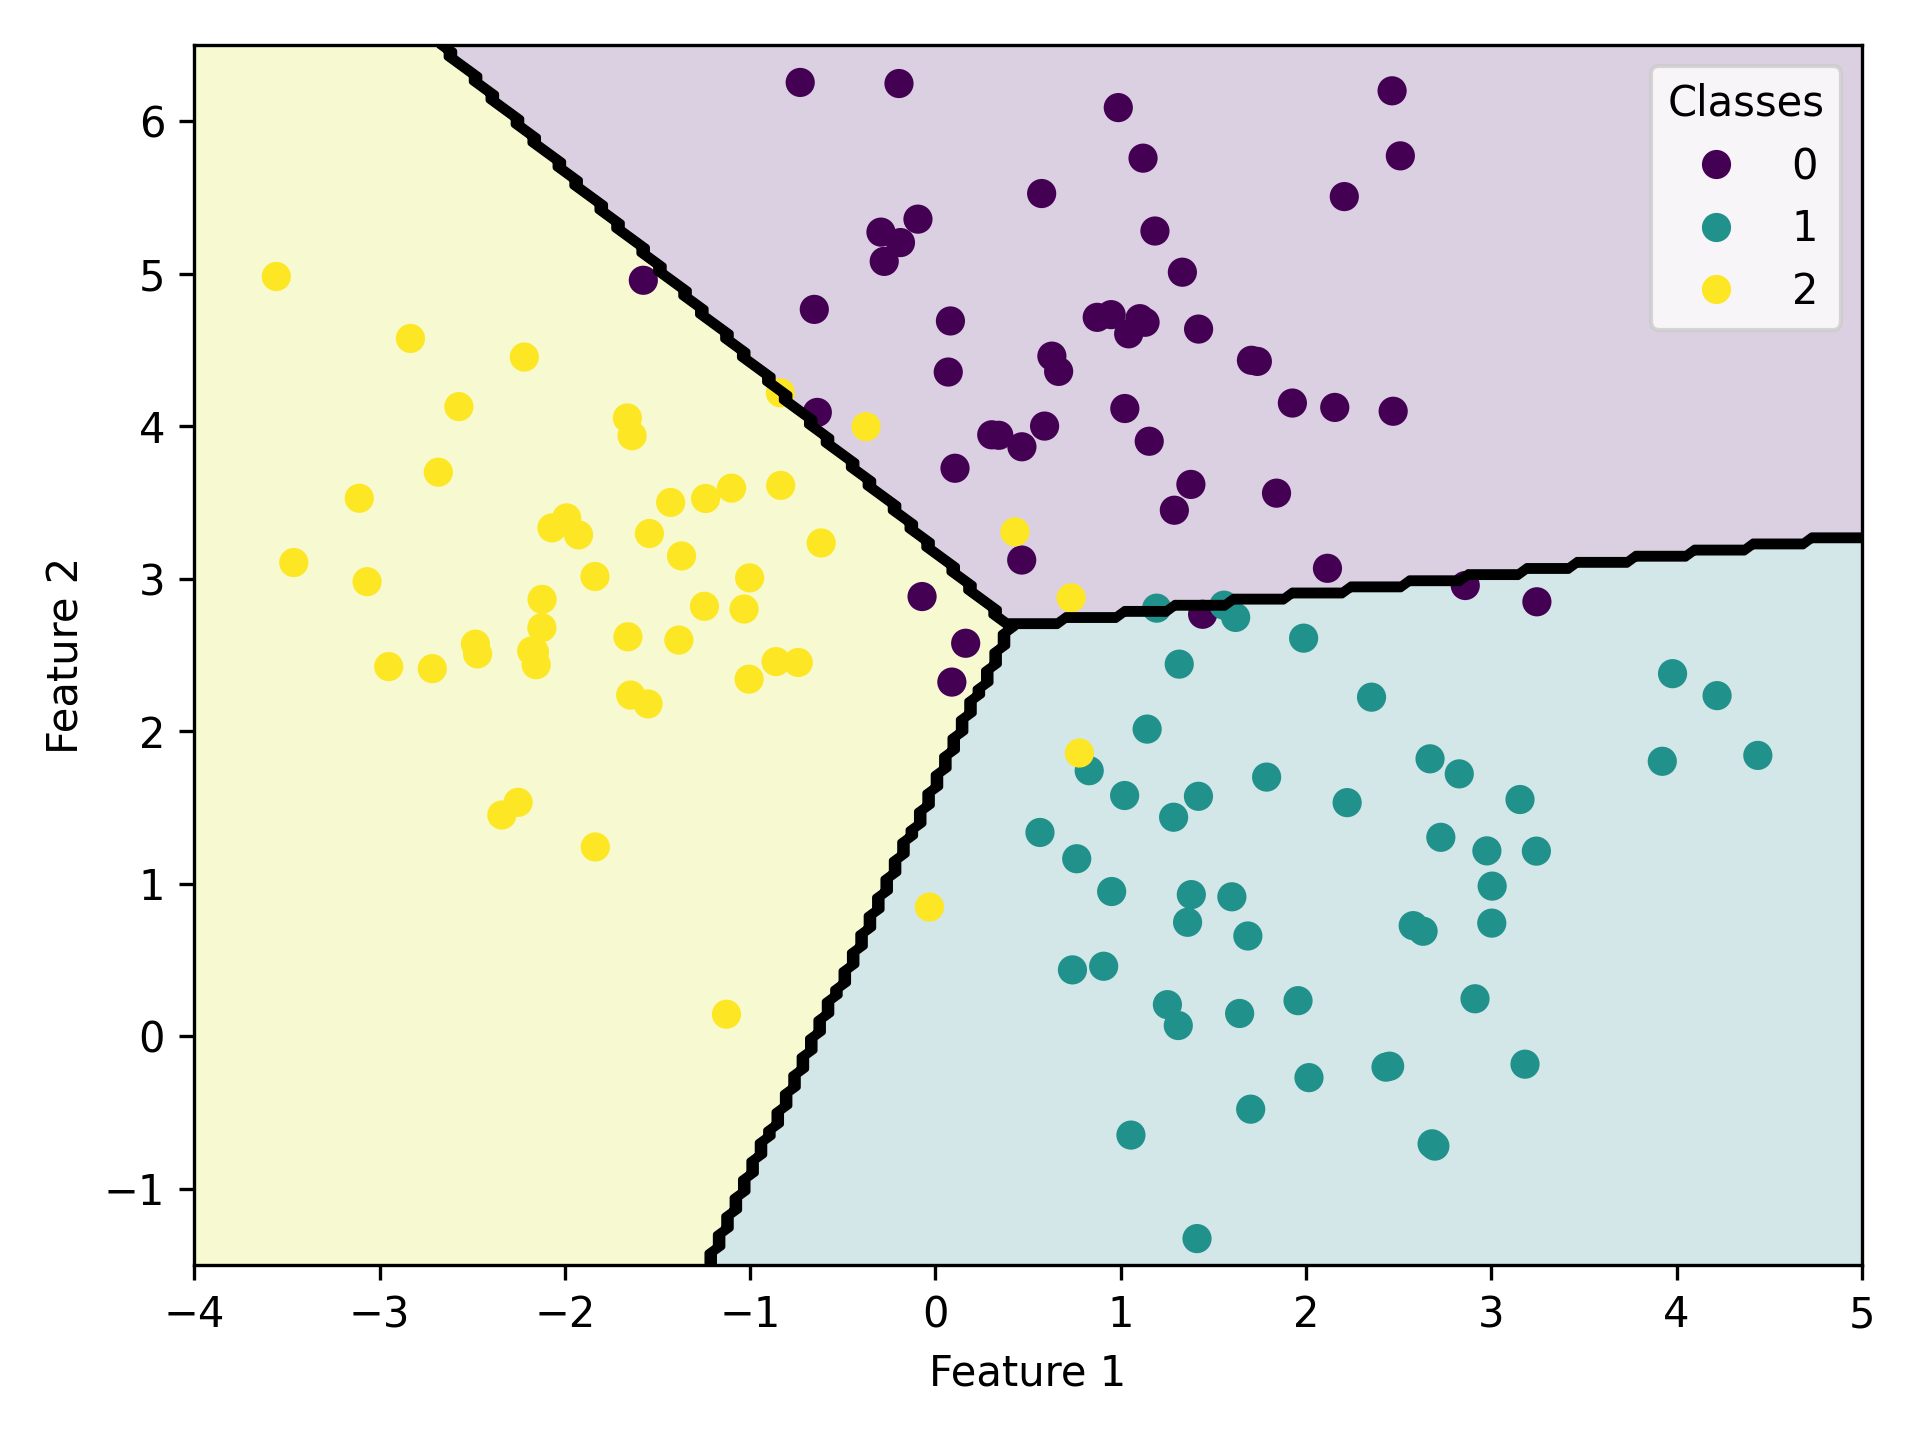
\includegraphics[width=\linewidth]{scatter_with_contour_B.png}
    \caption{Dataset B}
  \end{subfigure}
  \caption{Scatter plot of datasets colored by class with contour plots colored by predicted class.}
  \label{fig:pred}
\end{figure}

\subsubsection{Performance evaluation}

We used three metrics to evaluate our probabilistic generative model: Accuracy (Eq.\eqref{eq:accuracy}), Precision (Eq.\eqref{eq:precision}) and Recall (Eq.\eqref{eq:recall}).

\begin{equation}
\label{eq:accuracy}
Accuracy (\%) = \dfrac{TP}{P} \times 100\%
\end{equation}

\begin{equation}
  \label{eq:precision}
  Precision (\%) = \dfrac{TP}{TP+FP} \times 100\%
\end{equation}

\begin{equation}
  \label{eq:recall}
  Recall (\%) = \dfrac{TP}{TP+FN} \times 100\%
\end{equation}
where TP is the number of true positives, P is the number of positives, FP is the number of false positives and FN is the number of false positives.

The accuracy, precision and recall of our training and test sets are presented for dataset A and B in Table \ref{tab:2} and Table \ref{tab:3}, respectively.

\begin{table}[h]
  \centering
  \caption{Performance evaluation of dataset A.} \label{tab:2}
  \begin{tabular}{ccccccc}
  \cline{2-7}
   & \multicolumn{6}{c}{\textbf{Dataset A (\%)}} \\ \cline{2-7}
   & \multicolumn{3}{c}{\textbf{Training set}} & \multicolumn{3}{c}{\textbf{Test set}} \\ \hline
  \textbf{Classes} & \textbf{Accuracy} & \textbf{Precision} & \textbf{Recall} & \textbf{Accuracy} & \textbf{Precision} & \textbf{Recall} \\ \hline
  \textbf{0} & \multirow{3}{*}{79} & 84 & 84 & \multirow{3}{*}{73} & 71 & 85 \\ \cline{1-1} \cline{3-4} \cline{6-7} 
  \textbf{1} &  & 76 & 76 &  & 70 & 73 \\ \cline{1-1} \cline{3-4} \cline{6-7} 
  \textbf{2} &  & 76 & 76 &  & 82 & 61 \\ \hline
  \end{tabular}
\end{table}

\begin{table}[h]
  \centering
  \caption{Performance evaluation of dataset B.} \label{tab:3}
  \begin{tabular}{ccccccc}
  \cline{2-7}
   & \multicolumn{6}{c}{\textbf{Dataset B (\%)}} \\ \cline{2-7}
   & \multicolumn{3}{c}{\textbf{Training set}} & \multicolumn{3}{c}{\textbf{Test set}} \\ \hline
  \textbf{Classes} & \textbf{Accuracy} & \textbf{Precision} & \textbf{Recall} & \textbf{Accuracy} & \textbf{Precision} & \textbf{Recall} \\ \hline
  \textbf{0} & \multirow{3}{*}{88} & 91 & 80 & \multirow{3}{*}{95} & 92 & 92 \\ \cline{1-1} \cline{3-4} \cline{6-7} 
  \textbf{1} &  & 86 & 96 &  & 96 & 100 \\ \cline{1-1} \cline{3-4} \cline{6-7} 
  \textbf{2} &  & 88 & 88 &  & 96 & 92 \\ \hline
  \end{tabular}
  \end{table}

Our probabilistic generative model showed a reliable prediction performance, shown in our evaluation metrics. However, our model had some limitation when dealing with outliers. The Gaussian distribution fitted to the class-conditional probabilities are sensible to outliers, because the maximum likelihood estimation of a Guassian is not robust, as discussed by \cite{bishop2006}. Then, analyzing Fig. \ref{fig:pred}, we suggest that misclassified points could be outliers in their respective class. Probably a distribution robust to outliers, e. g. Laplace distribution, would yield a higher accuracy. Furthermore, the Gaussian with shared covariance matrix determine linear decision boundaries; however, we could have adopted individual covariances for each class, which would yield a quadratic decision boundary, what in some cases would improve our prediction capacity.

\section{Discriminative model}

\subsection{Data}

For the second experiment, we created a dataset composed by 100 data points divided equally in two classes, named as C (Fig. \ref{fig:data_discriminative}). The dataset was splited in the same way of the first experiment, with 50\% points in the training set and the remaining in the test set.

\begin{figure}[h]
  \centering
  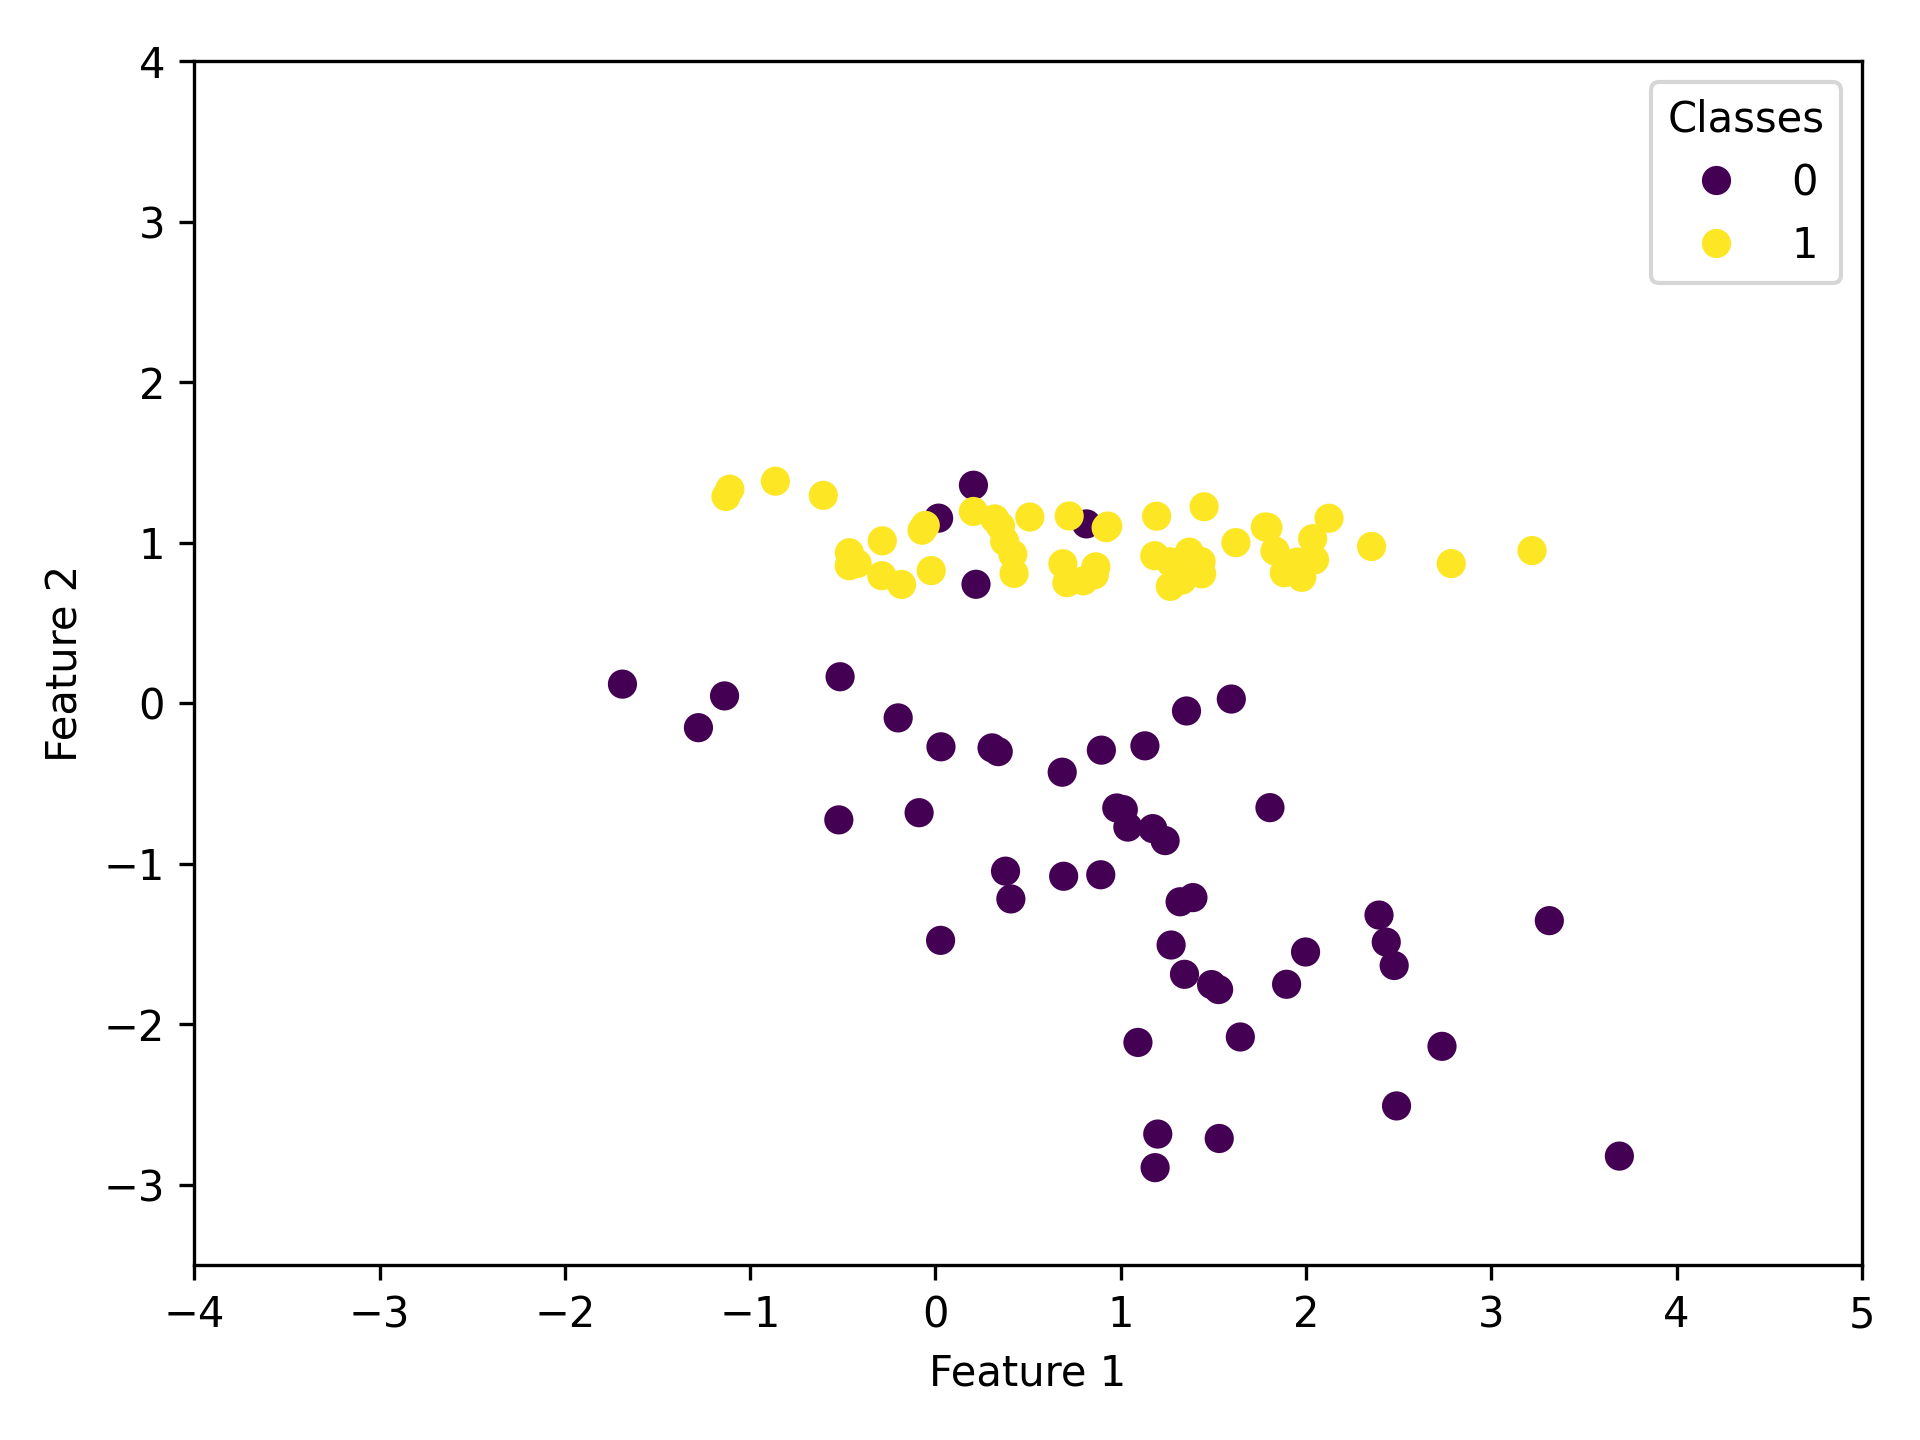
\includegraphics[width=0.49\linewidth]{scatter_3.png}
  \caption{Scatter plot of dataset C by class}
  \label{fig:data_discriminative}
\end{figure}

\subsection{Model}

Here, we shall implement a logistic regression to our two-class classification problem. We implemented a gradient descent algorithm to optimize the parameters of the logistic model and the Monte Carlo sampling to approximate it based on $S$ samples.

\subsubsection{Gradient Descent}

The gradient descent formula to optimize the parameter $w$ in a function $\ell$ is given by Eq.\eqref{eq:gradient_descent}, where $\alpha$ is the learning rate, that is, the size of each step. To obtain the function $\ell$, we must first define the hypothesis for the logistic regression, which is given by Eq.\eqref{eq:hypothesis}. Intuitively, we can define for $y$ being one by Eq.\eqref{eq:probBe1} and being zero by Eq.\eqref{eq:probBe2}.

\begin{equation}
  \label{eq:gradient_descent}
  w_{i+1} = w_{i} - \alpha \frac{\delta \ell(w_i)}{\delta w_i}
\end{equation}

\begin{equation}
  \label{eq:hypothesis}
  h(x) = \dfrac{1}{1 + e^{-W^{T} x}}
\end{equation}

\begin{equation}
  \label{eq:probBe1}
  p(y_i=1|x_i;W) = h(x_i)
\end{equation}

\begin{equation}
  \label{eq:probBe2}
  p(y_i=0|x_i;W) = 1 - h(x_i)
\end{equation}

We can use a Bernoulli distribution to join Eq.\eqref{eq:probBe1} and Eq.\eqref{eq:probBe2} to find the Eq.\eqref{eq:bernoulli}. We can see that for $y=1$ the term $h(x_i)^{y_i}$ becomes $h(x_i)$ and $(1 - h(x_i))^{1 - y_i}$ becomes 1, resulting in $h(x_i)$, and if $y=0$ the term $h(x_i)^{y_i}$ becomes 1 and the $(1 - h(x_i))^{1 - y_i}$ becomes $(1 - h(x_i))$, resulting in $(1 - h(x_i))$. We can obtain the likelihood from this equation obtaining \eqref{eq:generalBernoulli}.

\begin{equation}
  \label{eq:bernoulli}
  p(y_i|x_i;W) = h(x_i)^{y_i}(1 - h(x_i))^{1 - y_i} 
\end{equation}

\begin{equation}
  \label{eq:generalBernoulli}
  L(W) = \prod_{i=1}^{m} h(x_i)^{y_i}(1 - h(x_i))^{1 - y_i} 
\end{equation}

With likelihood equation, we obtain the log-likelihood (Eq.\eqref{eq:logBernoulli}) from it.

\begin{equation}
  \label{eq:logBernoulli}
  \ell(W) = \sum_{i=1}^{m} y_i\log{h(x_i)} + (1 - y_i)\log{(1 - h(x_i))} 
\end{equation}

Hence, we have to maximize the log-likelihood to optimize the parameters. To do so, we derive Eq.\eqref{eq:logBernoulli} in terms of the parameters $W$, obtaining the Eq.\eqref{eq:derivateW}.

\begin{equation}
  \label{eq:derivateW}
  \frac{\delta\ell(W)}{\delta W} = (Y - h(X))X
\end{equation}

Now, we return to Eq.\eqref{eq:gradient_descent} and replace the derivative, finally obtaining the Eq.\eqref{eq:gradient_descent_final}, in which we can optimize $W$.

\begin{equation}
  \label{eq:gradient_descent_final}
  w_{i+1} = w_{i} - \alpha (Y - h(X))X
\end{equation}

Finally, we will evaluate the effects of different learning rates on the performance of gradient descent algorithm. We apply learning rates ranging from $1e-7$ to 34.9.

\subsubsection{Prediction with Monte Carlo}

Knowing that the posterior is intractable, to obtain the uncertainty, we will use Monte Carlo, given the Eq.\eqref{eq:monte_carlo}. We will get the normal using $W$ as average and $W/10$ as covariance.

\begin{equation}
  \label{eq:monte_carlo}
  p(y=1|x, D) \approx \frac{1}{S}\sum_{s=1}^{S}h(x) 
\end{equation}

We will evaluate the effects of the sample size on the performance of the Monte Carlo sampling. We apply the following sample sizes: 100, 1000, 10000 and 100000

\subsubsection{Results}

First, we ploted the loss function versus the learning rate (Fig. \ref{fig:learning_rates}). We observed that, for a small learning rate, i.e. between $1e-7$ and $1e-5$, the loss function does not converge in a reasonable time. Between $1e-5$ and 10, the loss function decreases constantly, which represents a good choice of learning rate, and between 10 and 34.9, the loss function diverges. Based on this, we chose the values of $1e-7$, $1e-3$ and 34.9 to be the values of learning rate to be tested, using an example of each part of the curve.

We plotted all results of the test set with the varying learning rates and samples sizes, as previously mentioned, in the Fig. \ref{fig:discriminative_results}. We noted that the linear decision boundary was incorrectly fitted for a very small learning rate, sucessfully fitted for a middle and large learning rates, with some small differences between them, which was expected. In addition, the performance metrics, such as accuracy, precision and recall, are showed in the Tables 4 to 15. As shown, the most part of the configurations predicted the classes sucessfully for a middle and large learning rates, and incorrectly for a very small learning rate, achieving reasonable metrics.

We also plotted the histograms of $W$ for bias, Feature 1 and Feature 2 are shown in Figs. \ref{fig:hist_featbias}, \ref{fig:hist_feat0} and \ref{fig:hist_feat1}, respectively. As observed, with a small number of samples, the histogram does not resembles a Gaussian distribution, which is expected. Then, with a increasing number of samples, the histogram also increases its resemblance to a Gaussian distribution. Therefore, the sample size $S$ yield good approximations if it is able to properly describe the real distribution of $W$. 

\begin{figure}
  \centering
  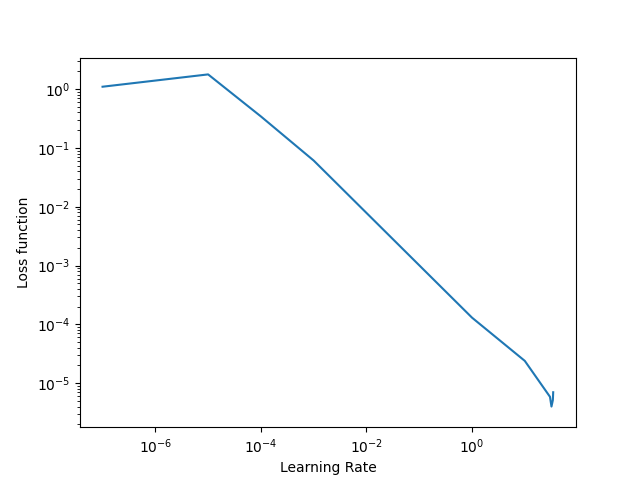
\includegraphics[width=0.6\linewidth]{learning_rates.png}
  \caption{Loss function with different learning rates.}
  \label{fig:learning_rates}
\end{figure}

% Scatter plot - discriminative
\begin{figure}
  \centering
  \begin{subfigure}[t]{0.24\textwidth}
    \centering
    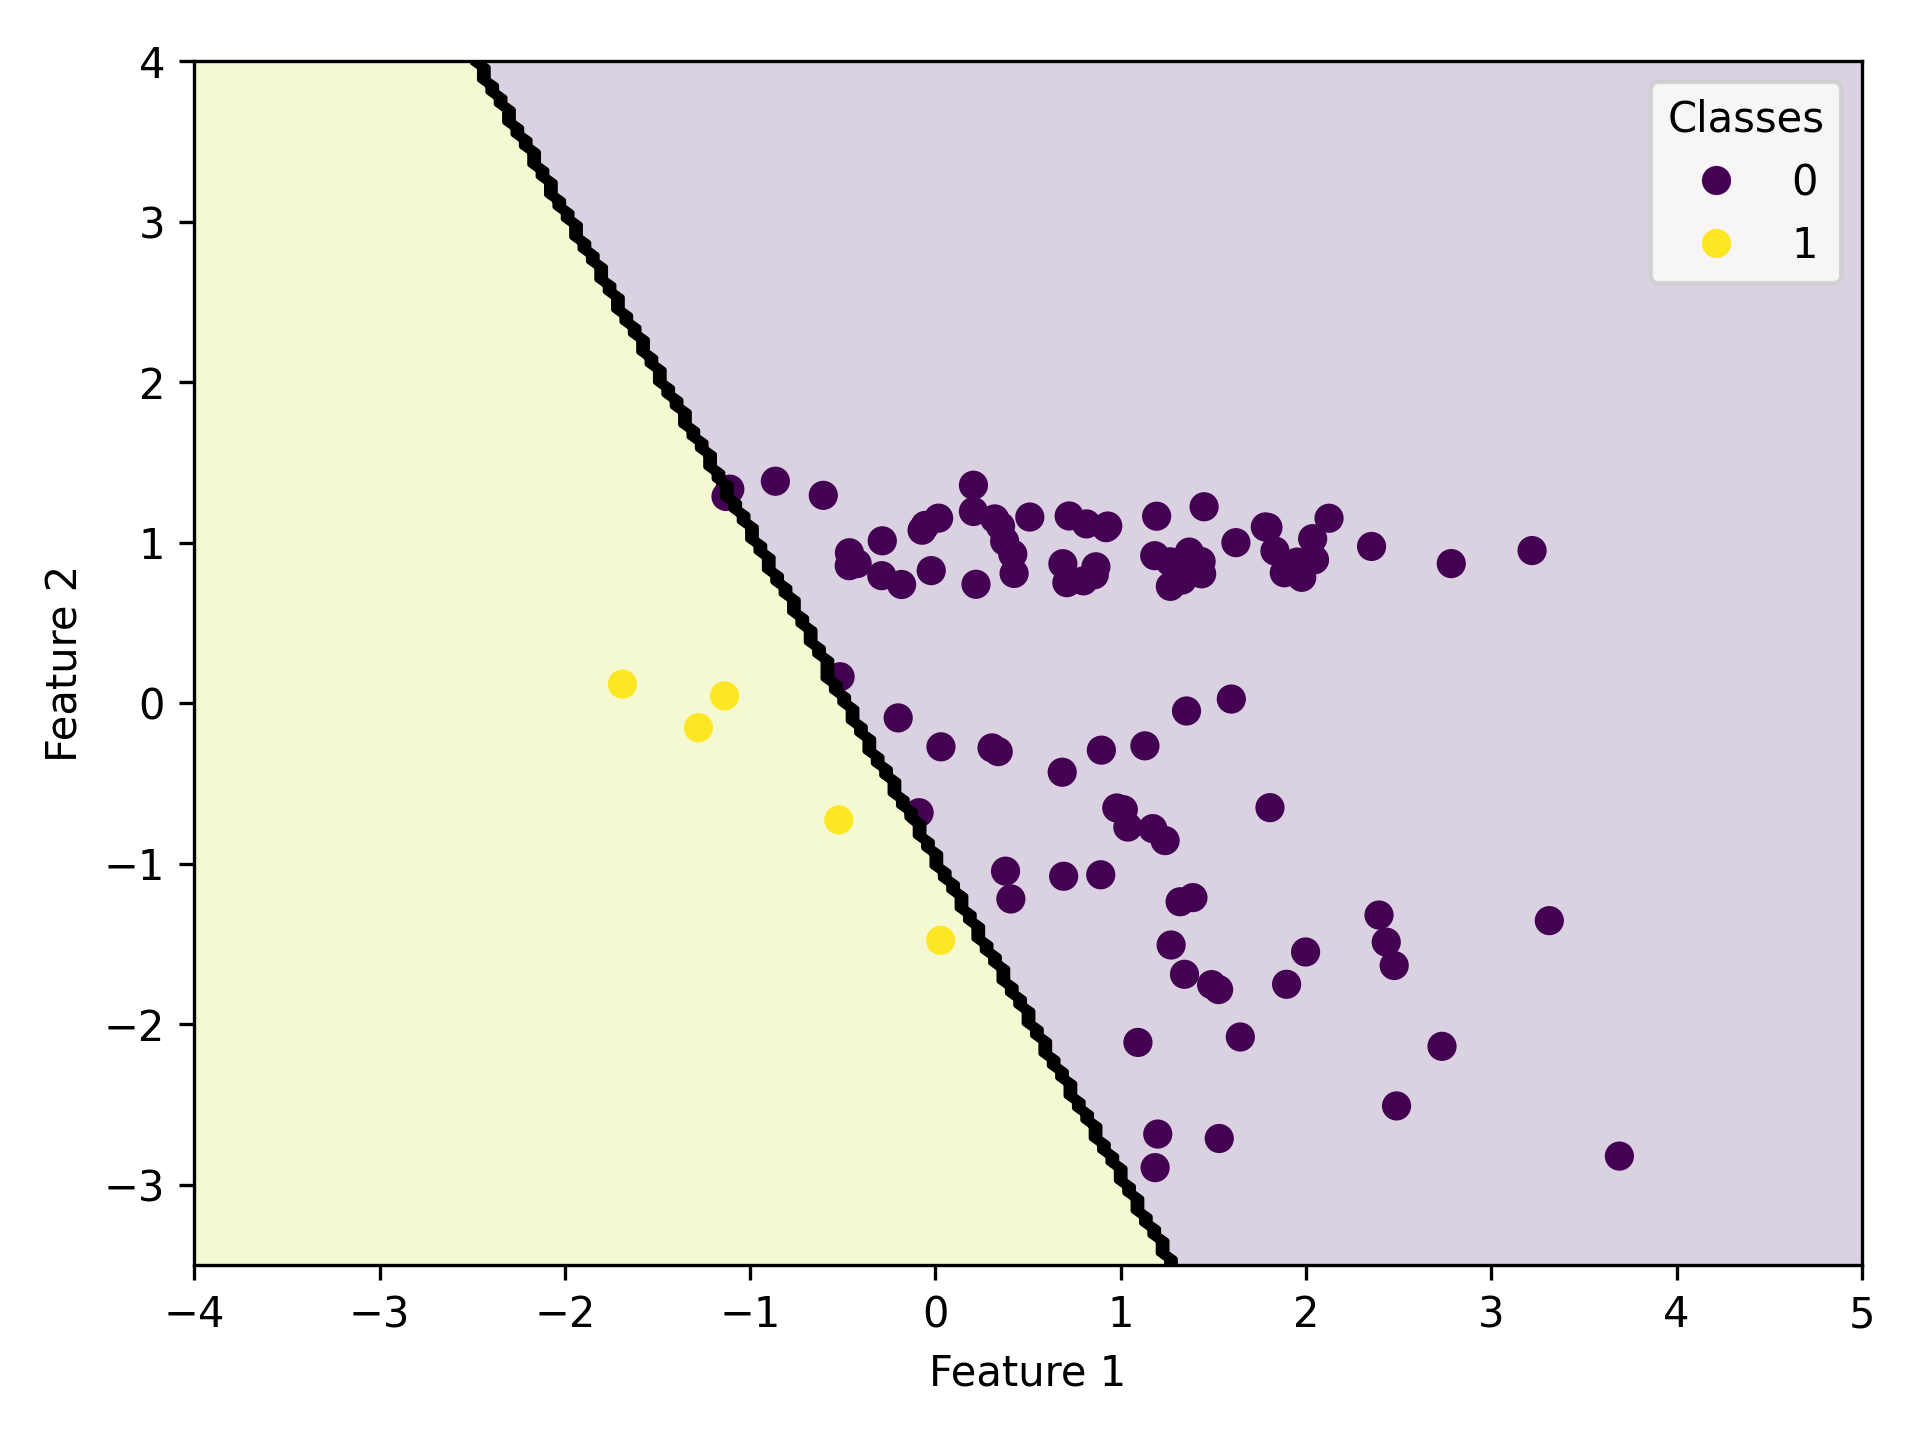
\includegraphics[width=\linewidth]{scatter_predictions_with_contour_3_learning_rate_1_sample_100.png}
    \caption{$\alpha = 1e-7$; $S = 100$.}
  \end{subfigure}
  \hfill
  \begin{subfigure}[t]{0.24\textwidth}
    \centering
    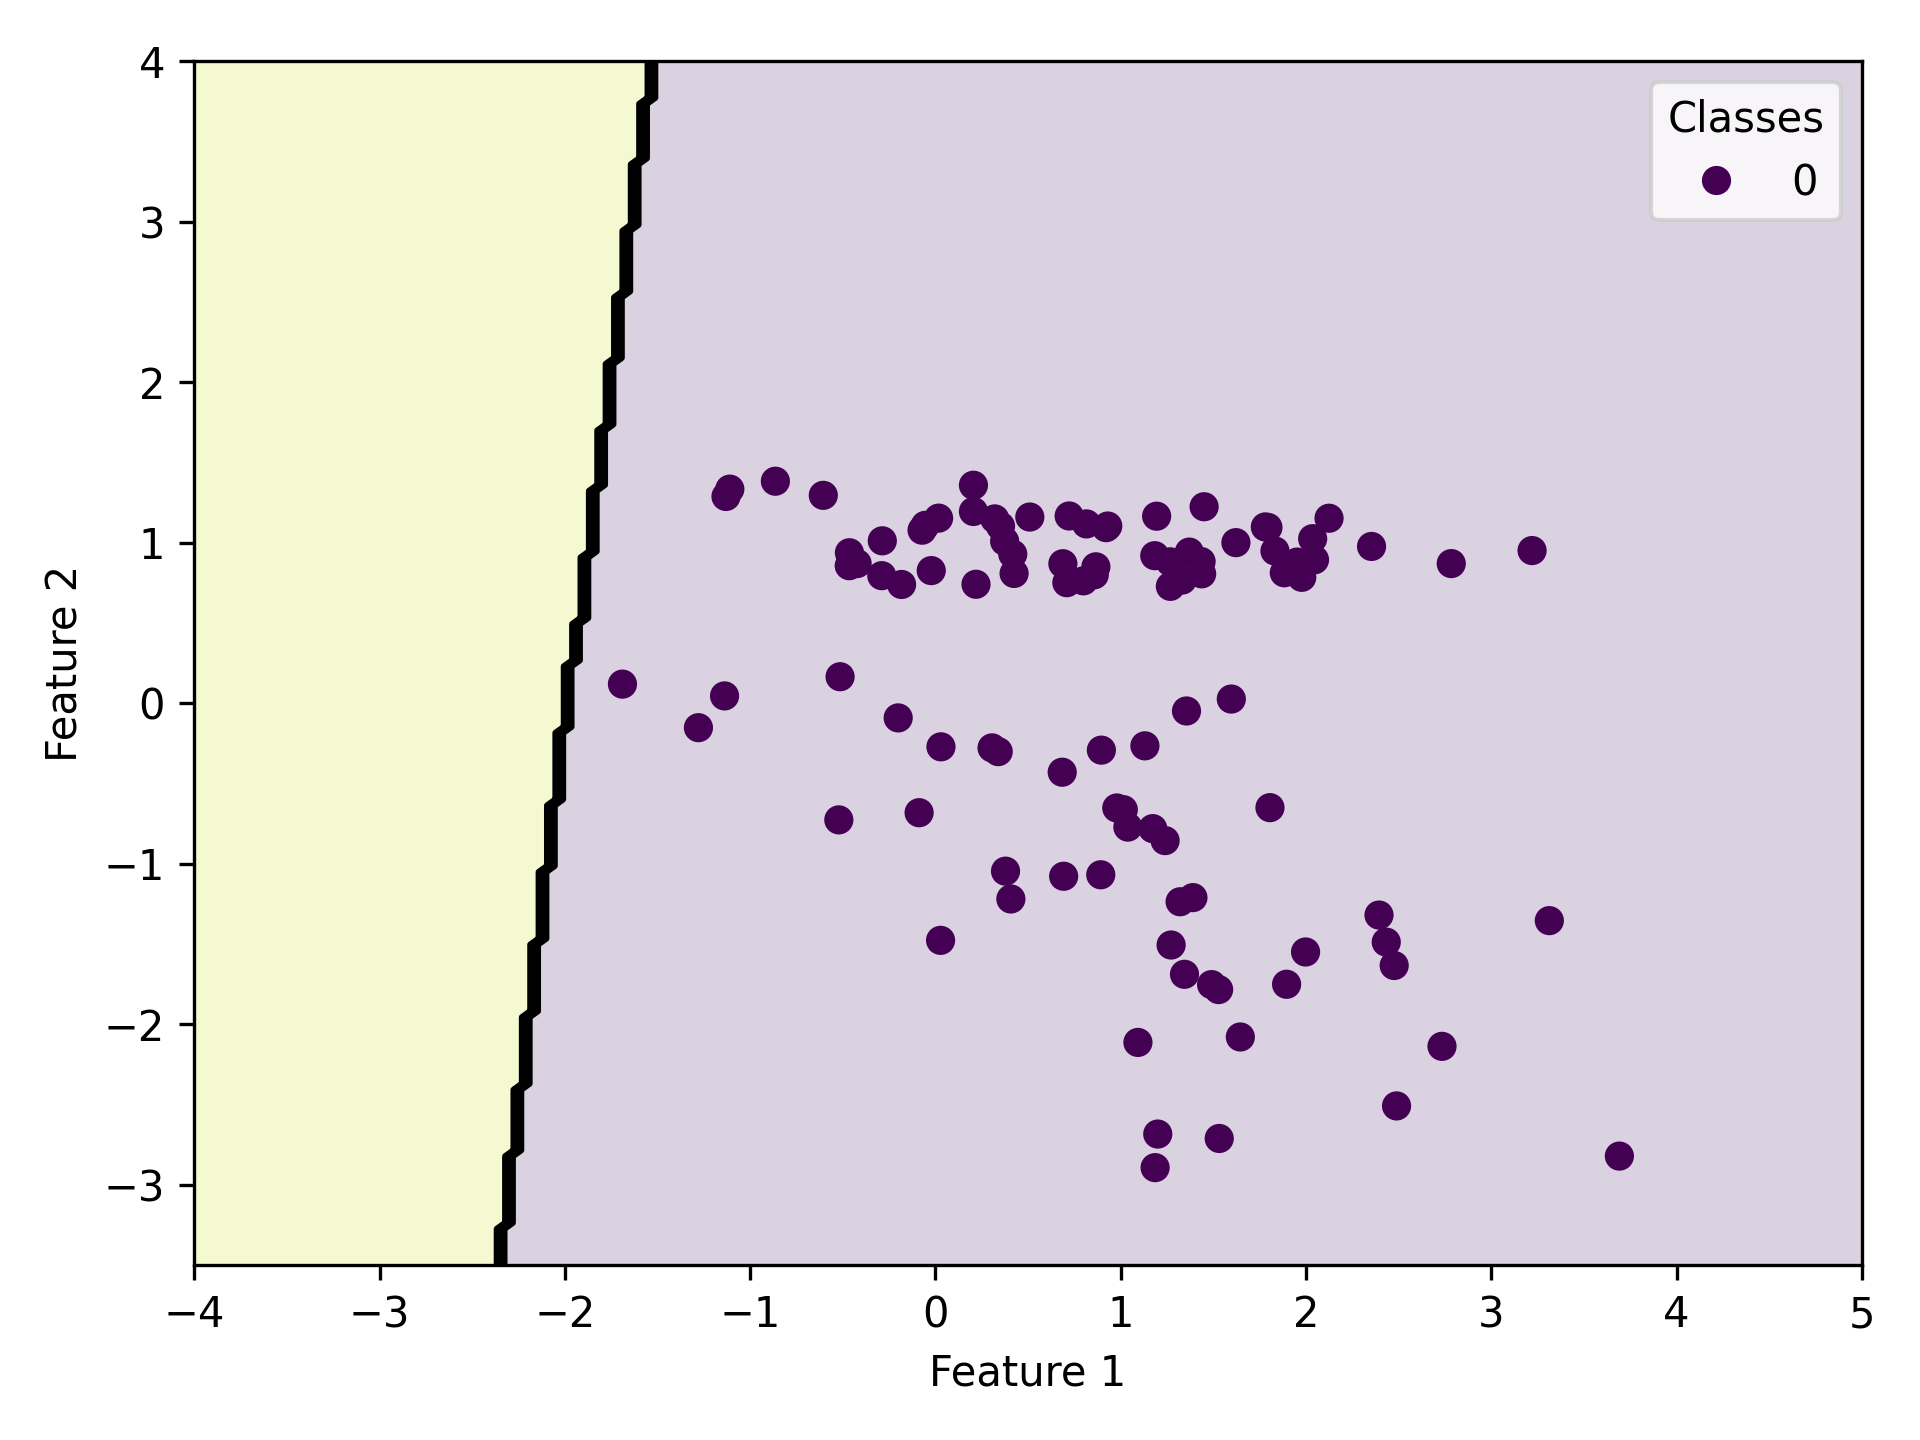
\includegraphics[width=\linewidth]{scatter_predictions_with_contour_3_learning_rate_1_sample_1000.png}
    \caption{$\alpha = 1e-7$; $S = 1000$.}
  \end{subfigure}
  \hfill
  \begin{subfigure}[t]{0.24\textwidth}
    \centering
    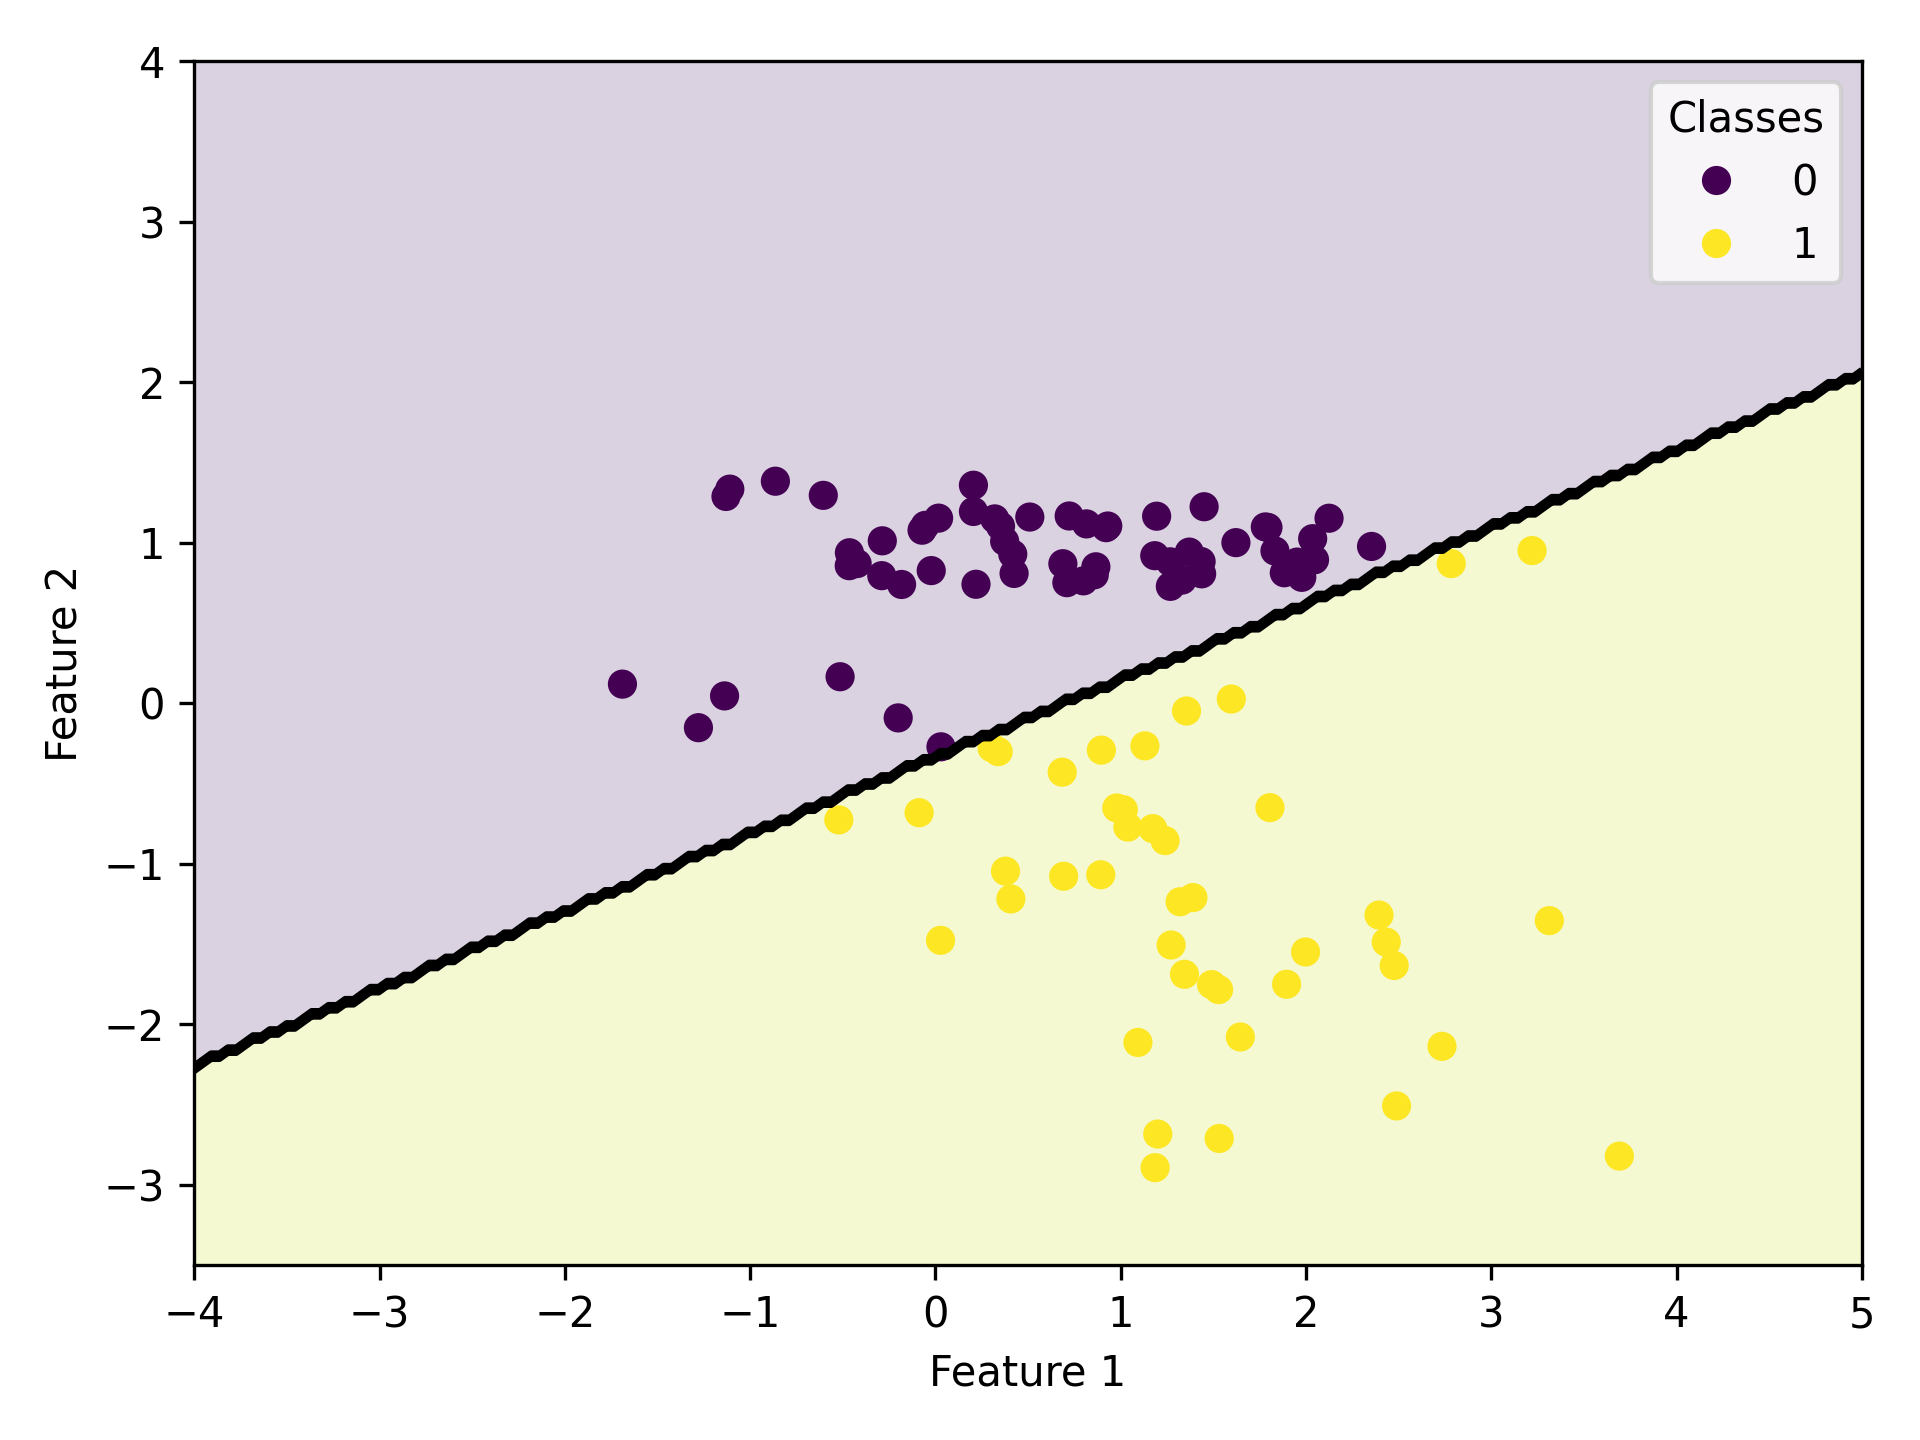
\includegraphics[width=\linewidth]{scatter_predictions_with_contour_3_learning_rate_1_sample_10000.png}
    \caption{$\alpha = 1e-7$; $S = 10000$.}
  \end{subfigure}
  \hfill
  \begin{subfigure}[t]{0.24\textwidth}
    \centering
    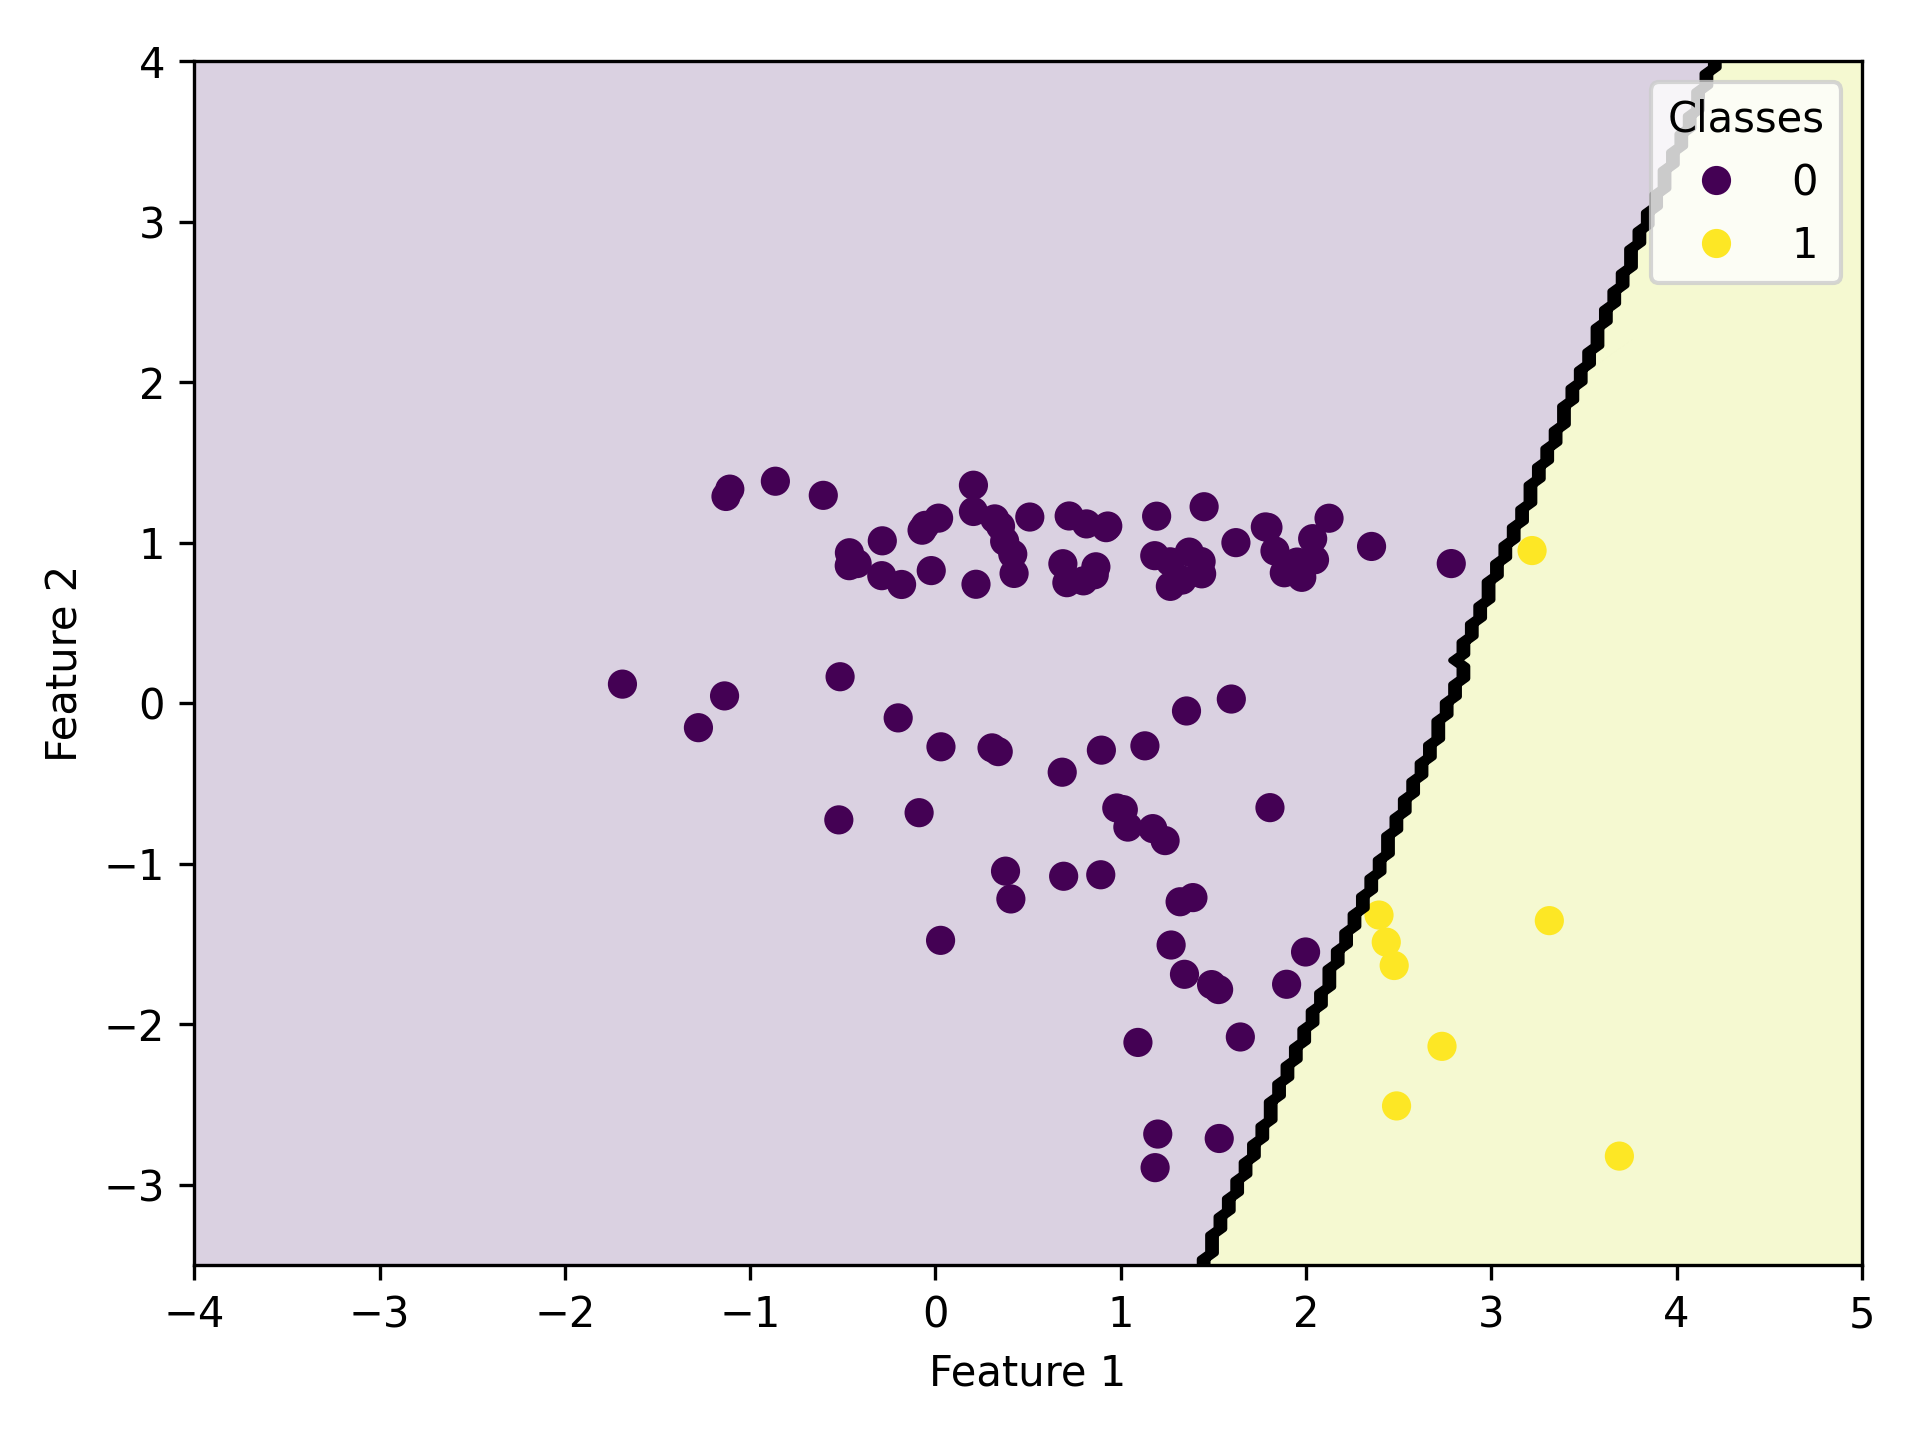
\includegraphics[width=\linewidth]{scatter_predictions_with_contour_3_learning_rate_1_sample_100000.png}
    \caption{$\alpha = 1e-7$; $S = 100000$.}
  \end{subfigure}
  % \hfill
  \begin{subfigure}[t]{0.24\textwidth}
    \centering
    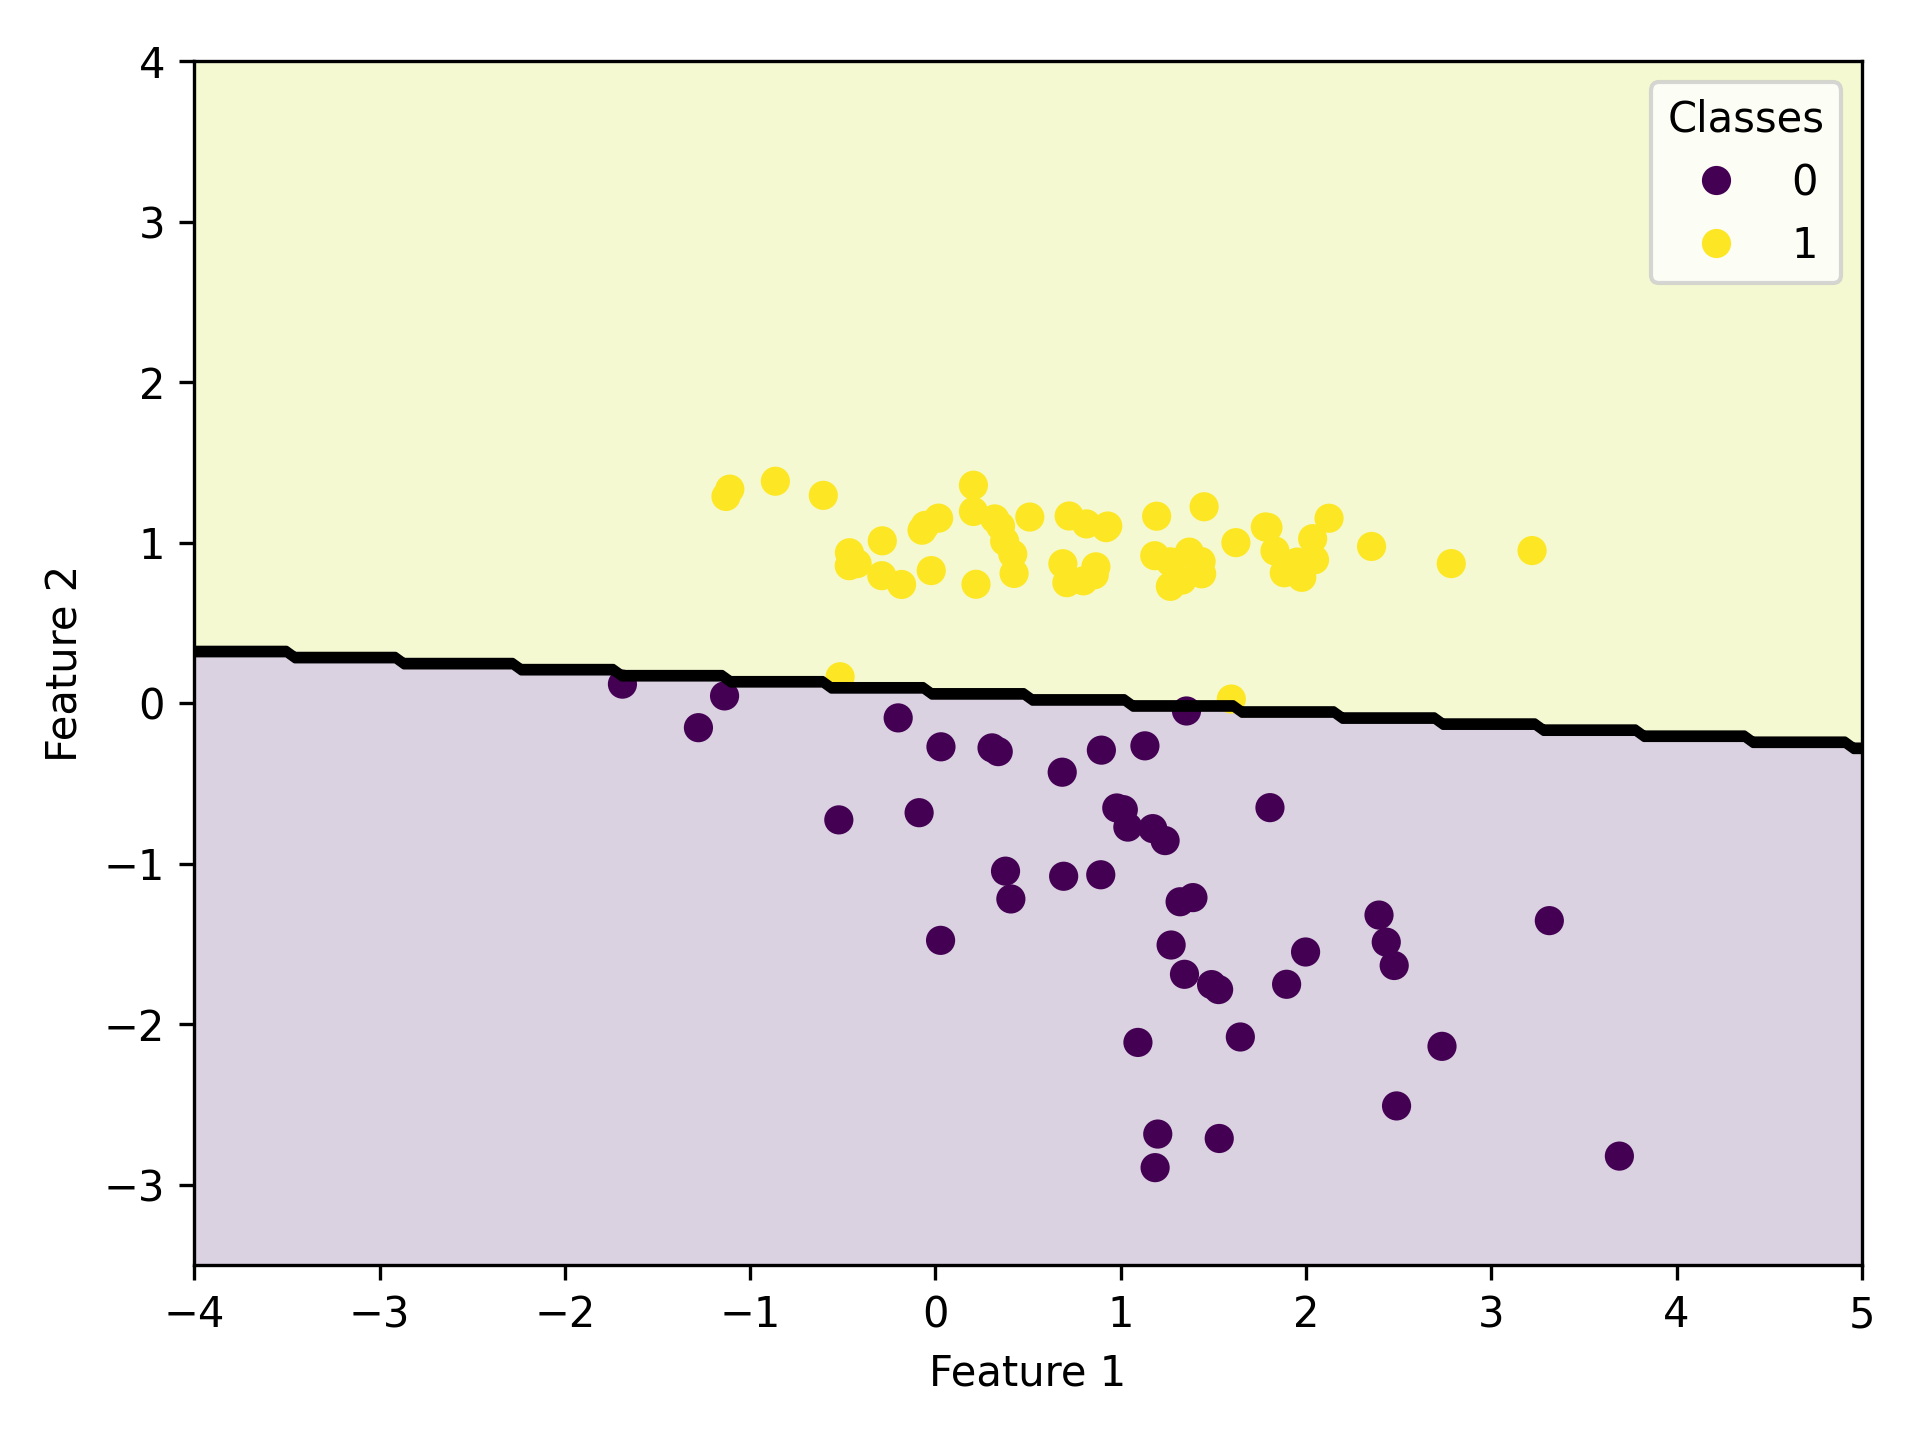
\includegraphics[width=\linewidth]{scatter_predictions_with_contour_3_learning_rate_10000_sample_100.png}
    \caption{$\alpha = 1e-3$; $S = 100$.}
  \end{subfigure}
  \hfill
  \begin{subfigure}[t]{0.24\textwidth}
    \centering
    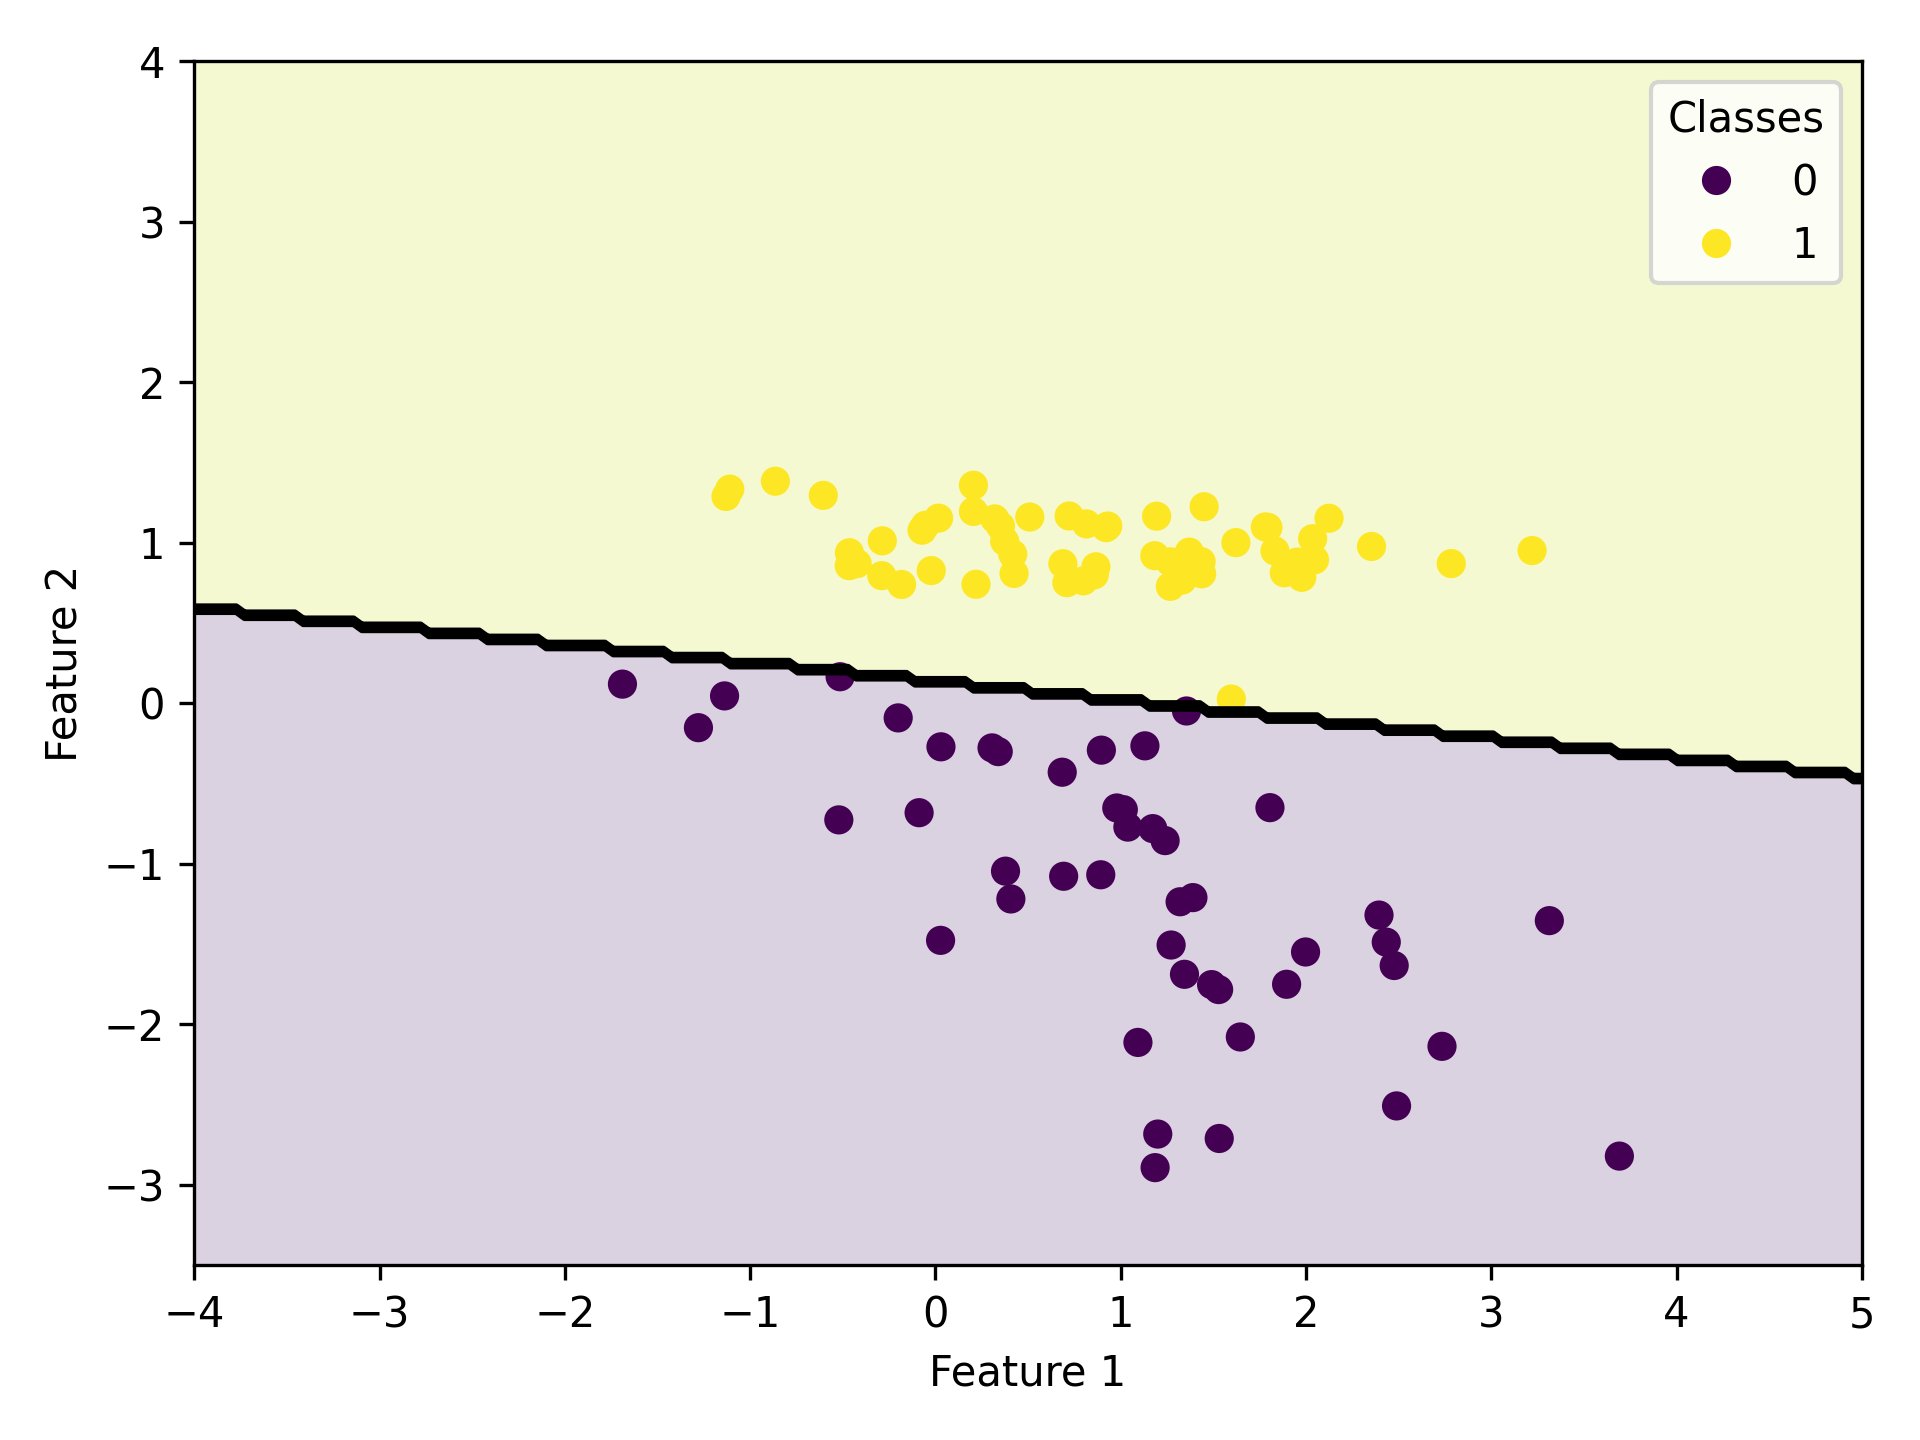
\includegraphics[width=\linewidth]{scatter_predictions_with_contour_3_learning_rate_10000_sample_1000.png}
    \caption{$\alpha = 1e-3$; $S = 1000$.}
  \end{subfigure}
  \hfill
  \begin{subfigure}[t]{0.24\textwidth}
    \centering
    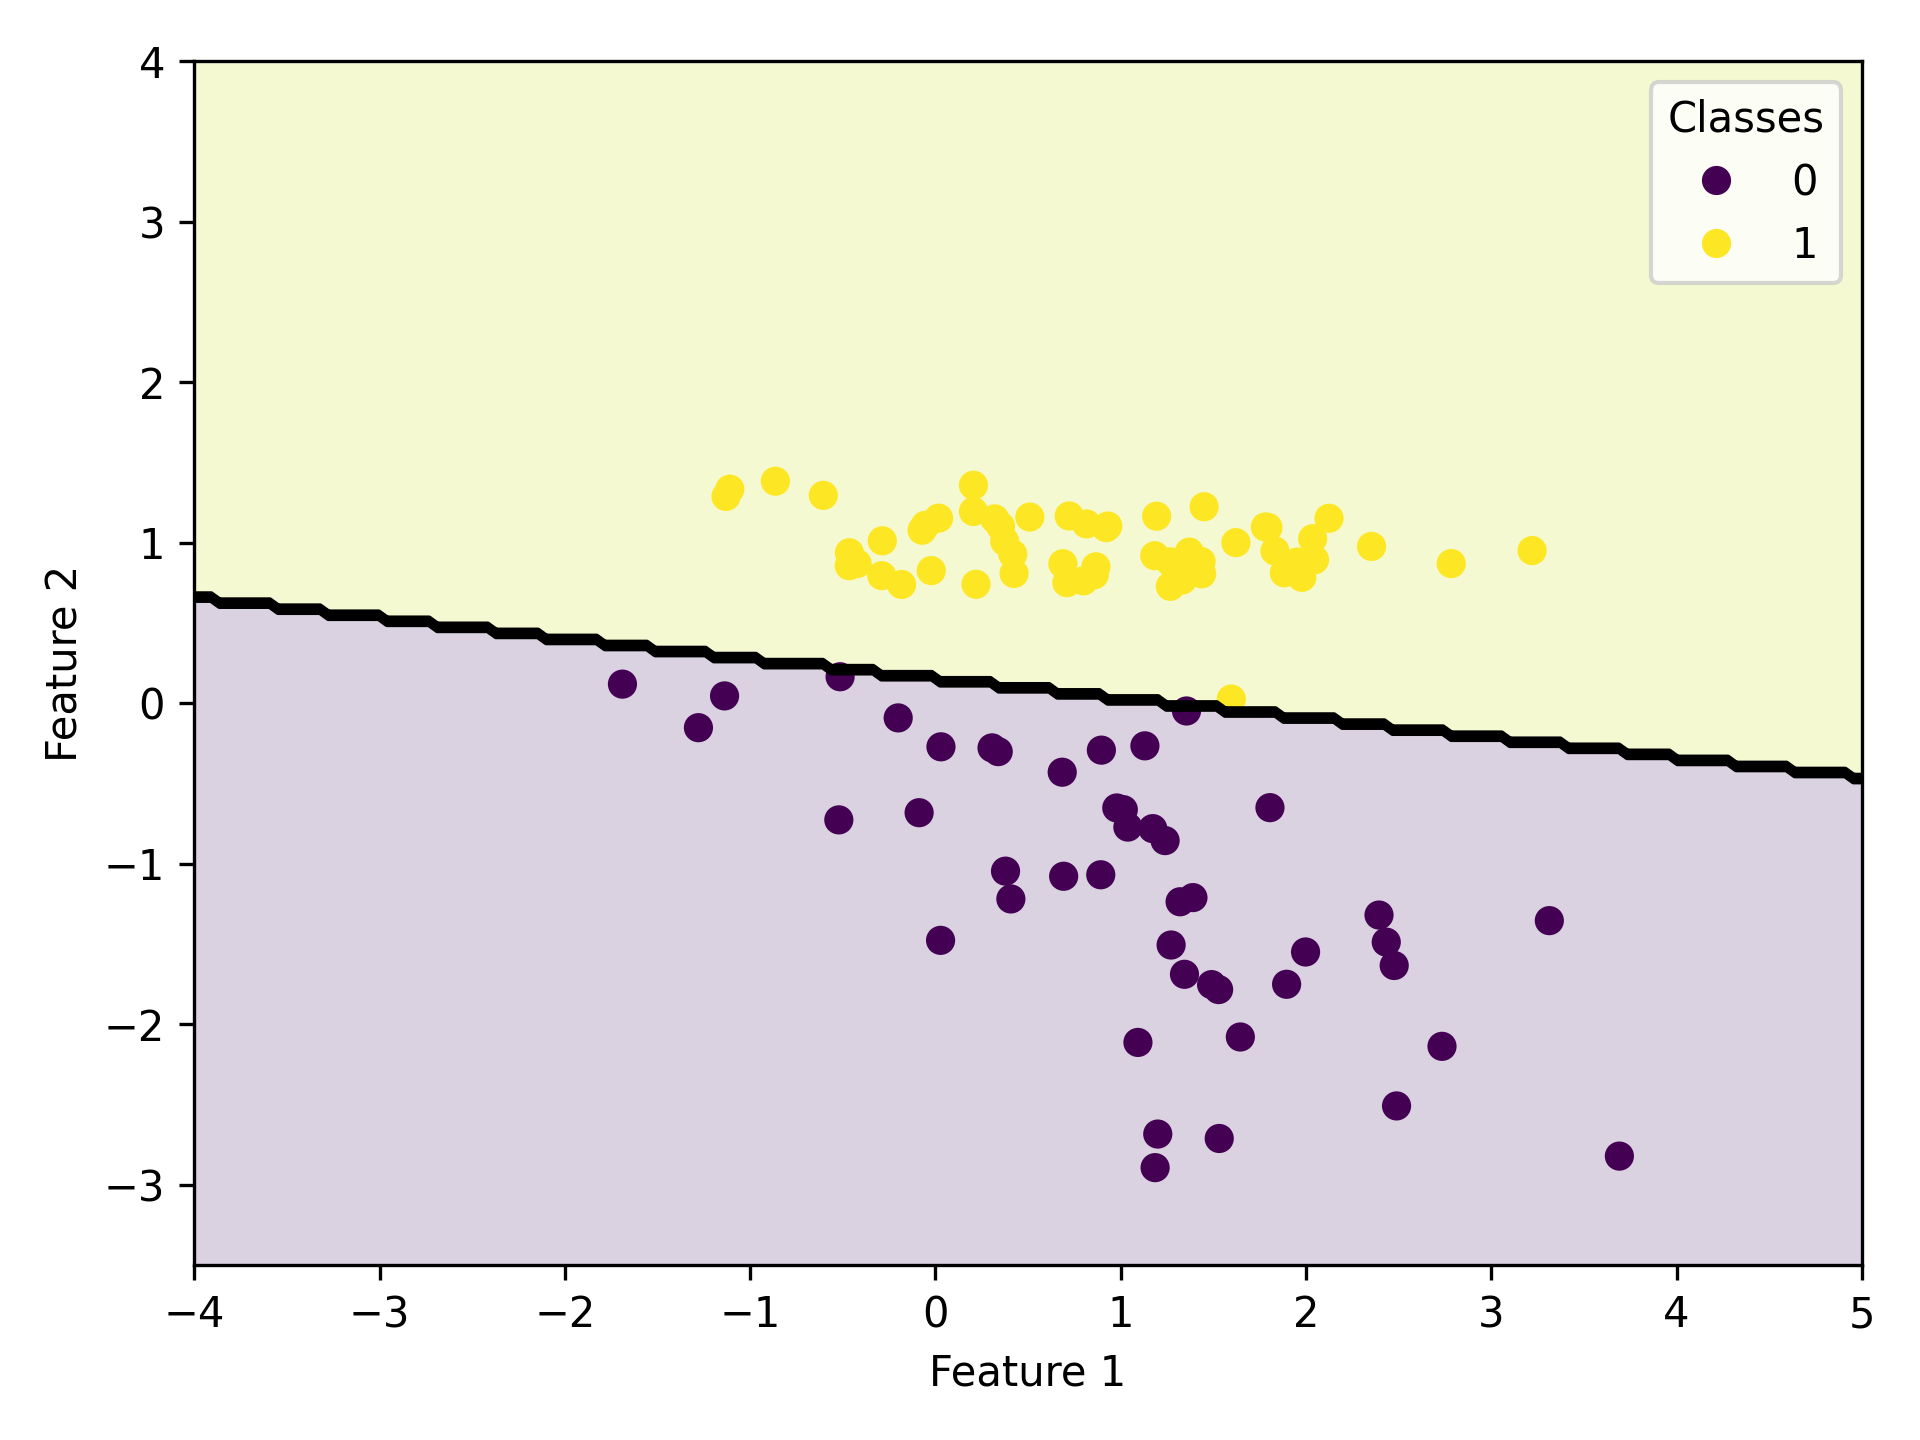
\includegraphics[width=\linewidth]{scatter_predictions_with_contour_3_learning_rate_10000_sample_10000.png}
    \caption{$\alpha = 1e-3$; $S = 10000$.}
  \end{subfigure}
  \hfill
  \begin{subfigure}[t]{0.24\textwidth}
    \centering
    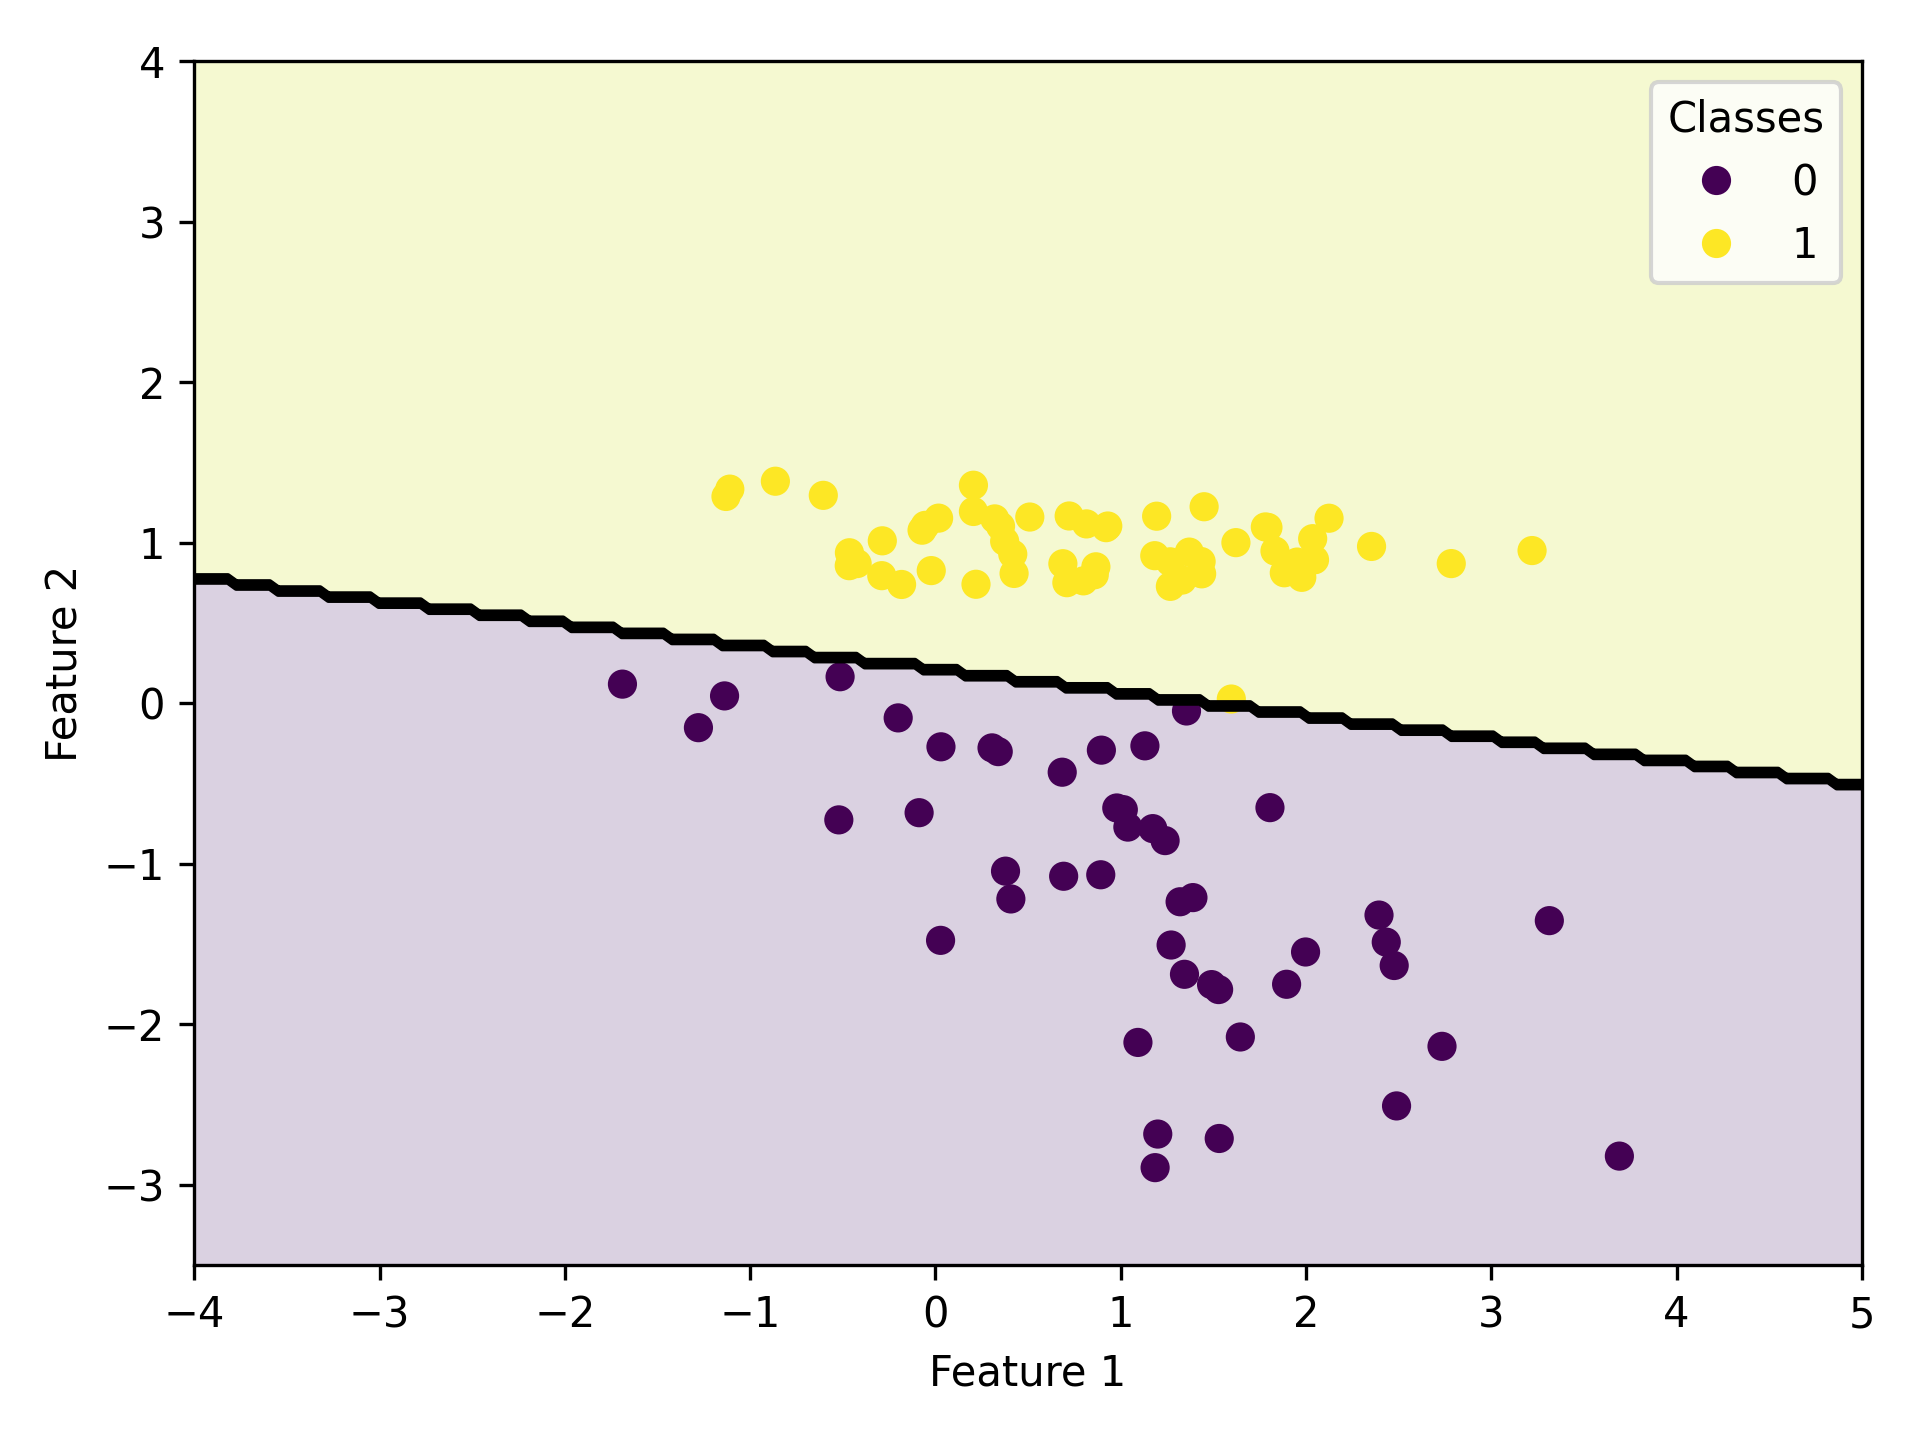
\includegraphics[width=\linewidth]{scatter_predictions_with_contour_3_learning_rate_10000_sample_100000.png}
    \caption{$\alpha = 1e-3$; $S = 100000$.}
  \end{subfigure}
  % \hfill
  \begin{subfigure}[t]{0.24\textwidth}
    \centering
    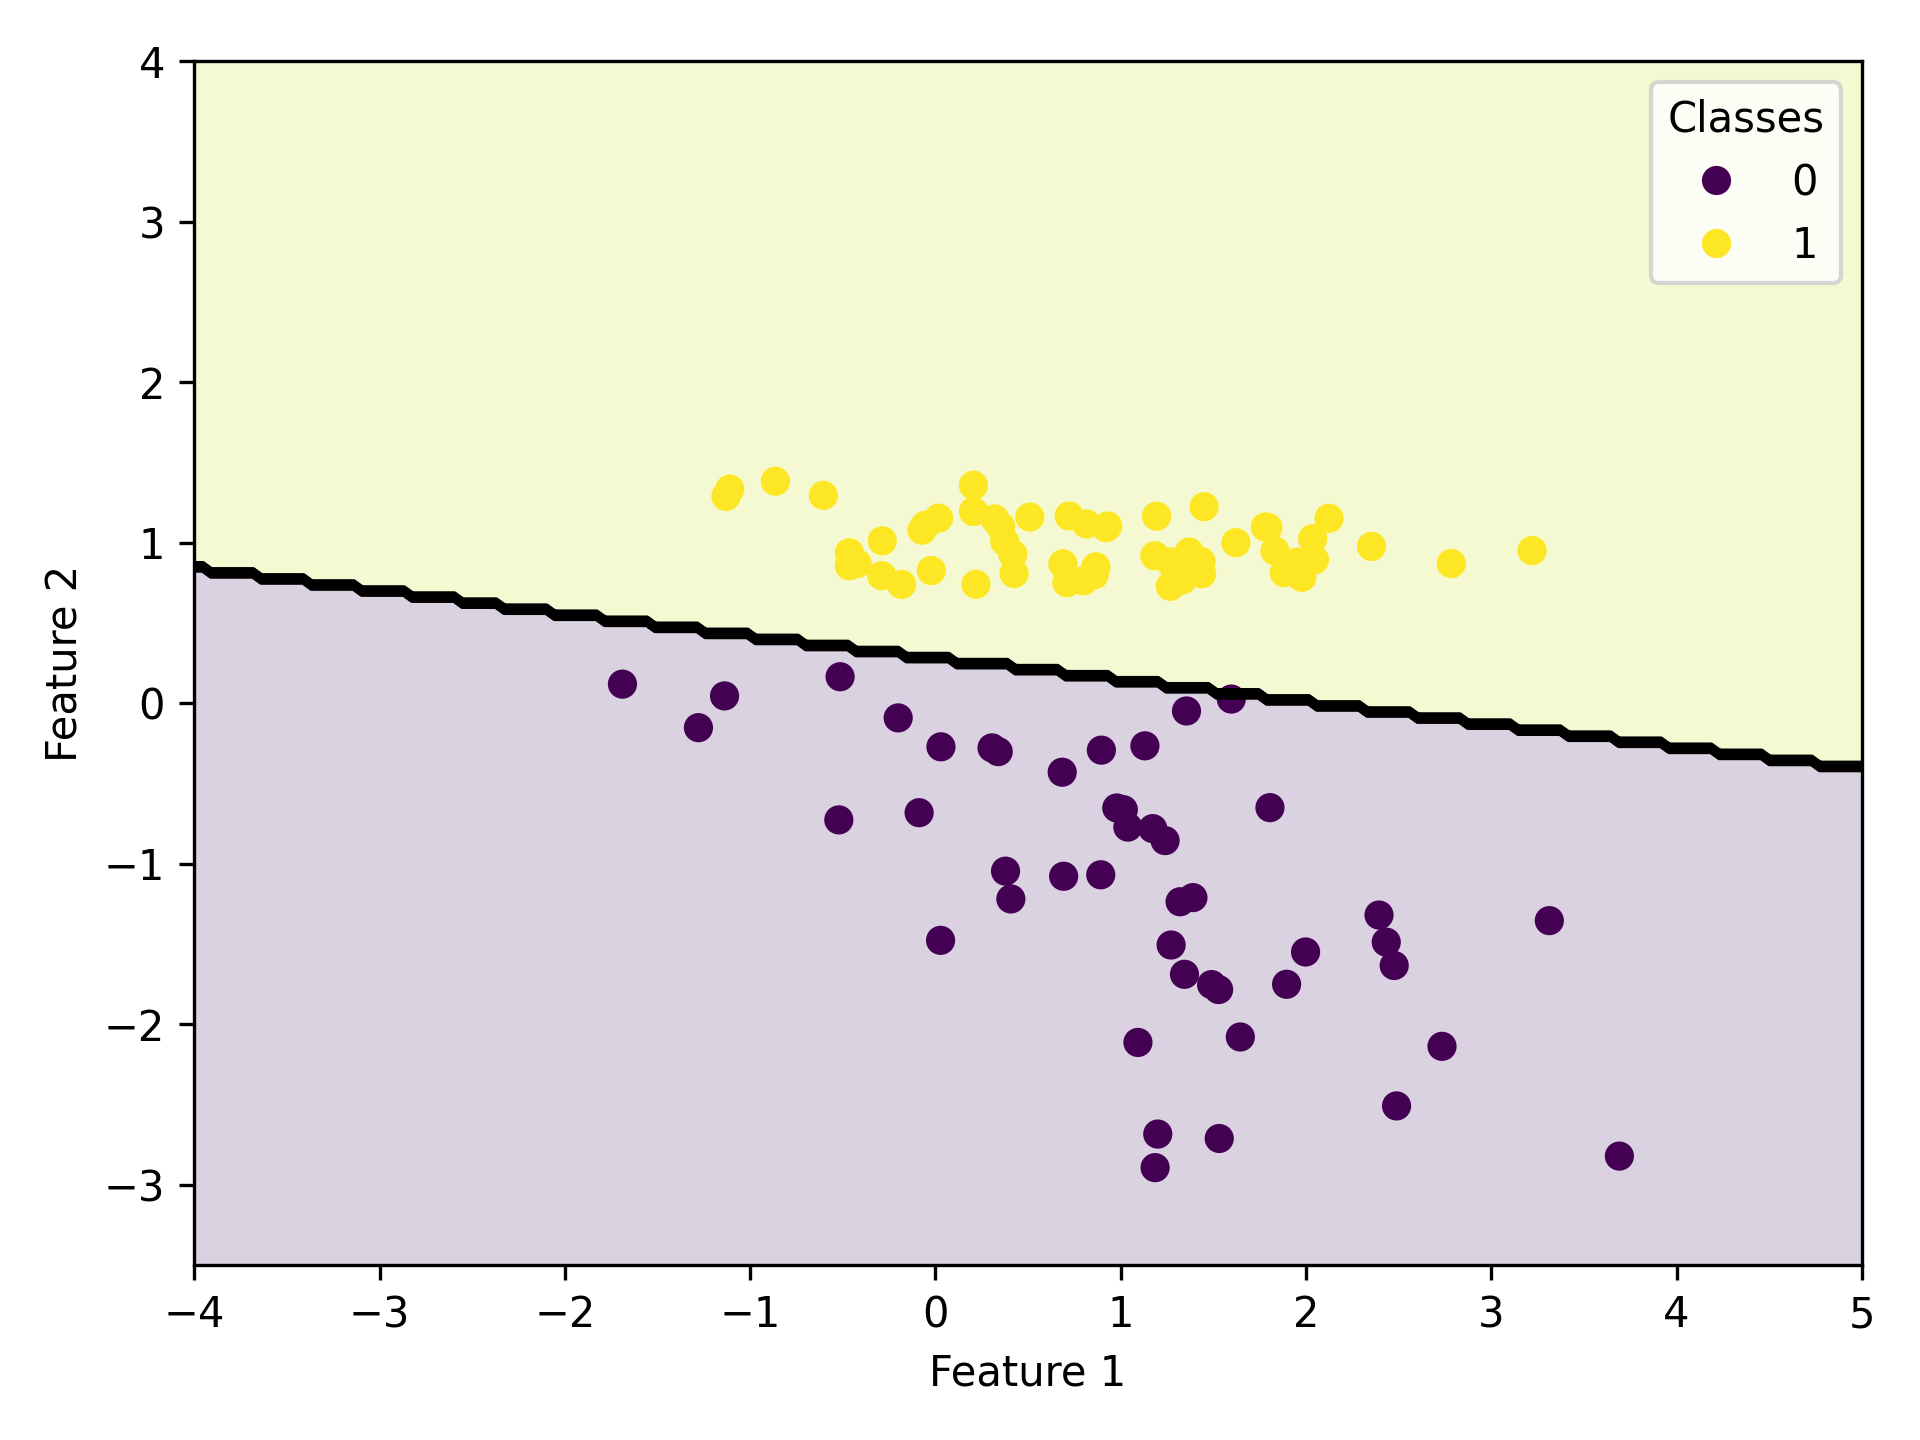
\includegraphics[width=\linewidth]{scatter_predictions_with_contour_3_learning_rate_349000000_sample_100.png}
    \caption{$\alpha = 34.9$; $S = 100$.}
  \end{subfigure}
  \hfill
  \begin{subfigure}[t]{0.24\textwidth}
    \centering
    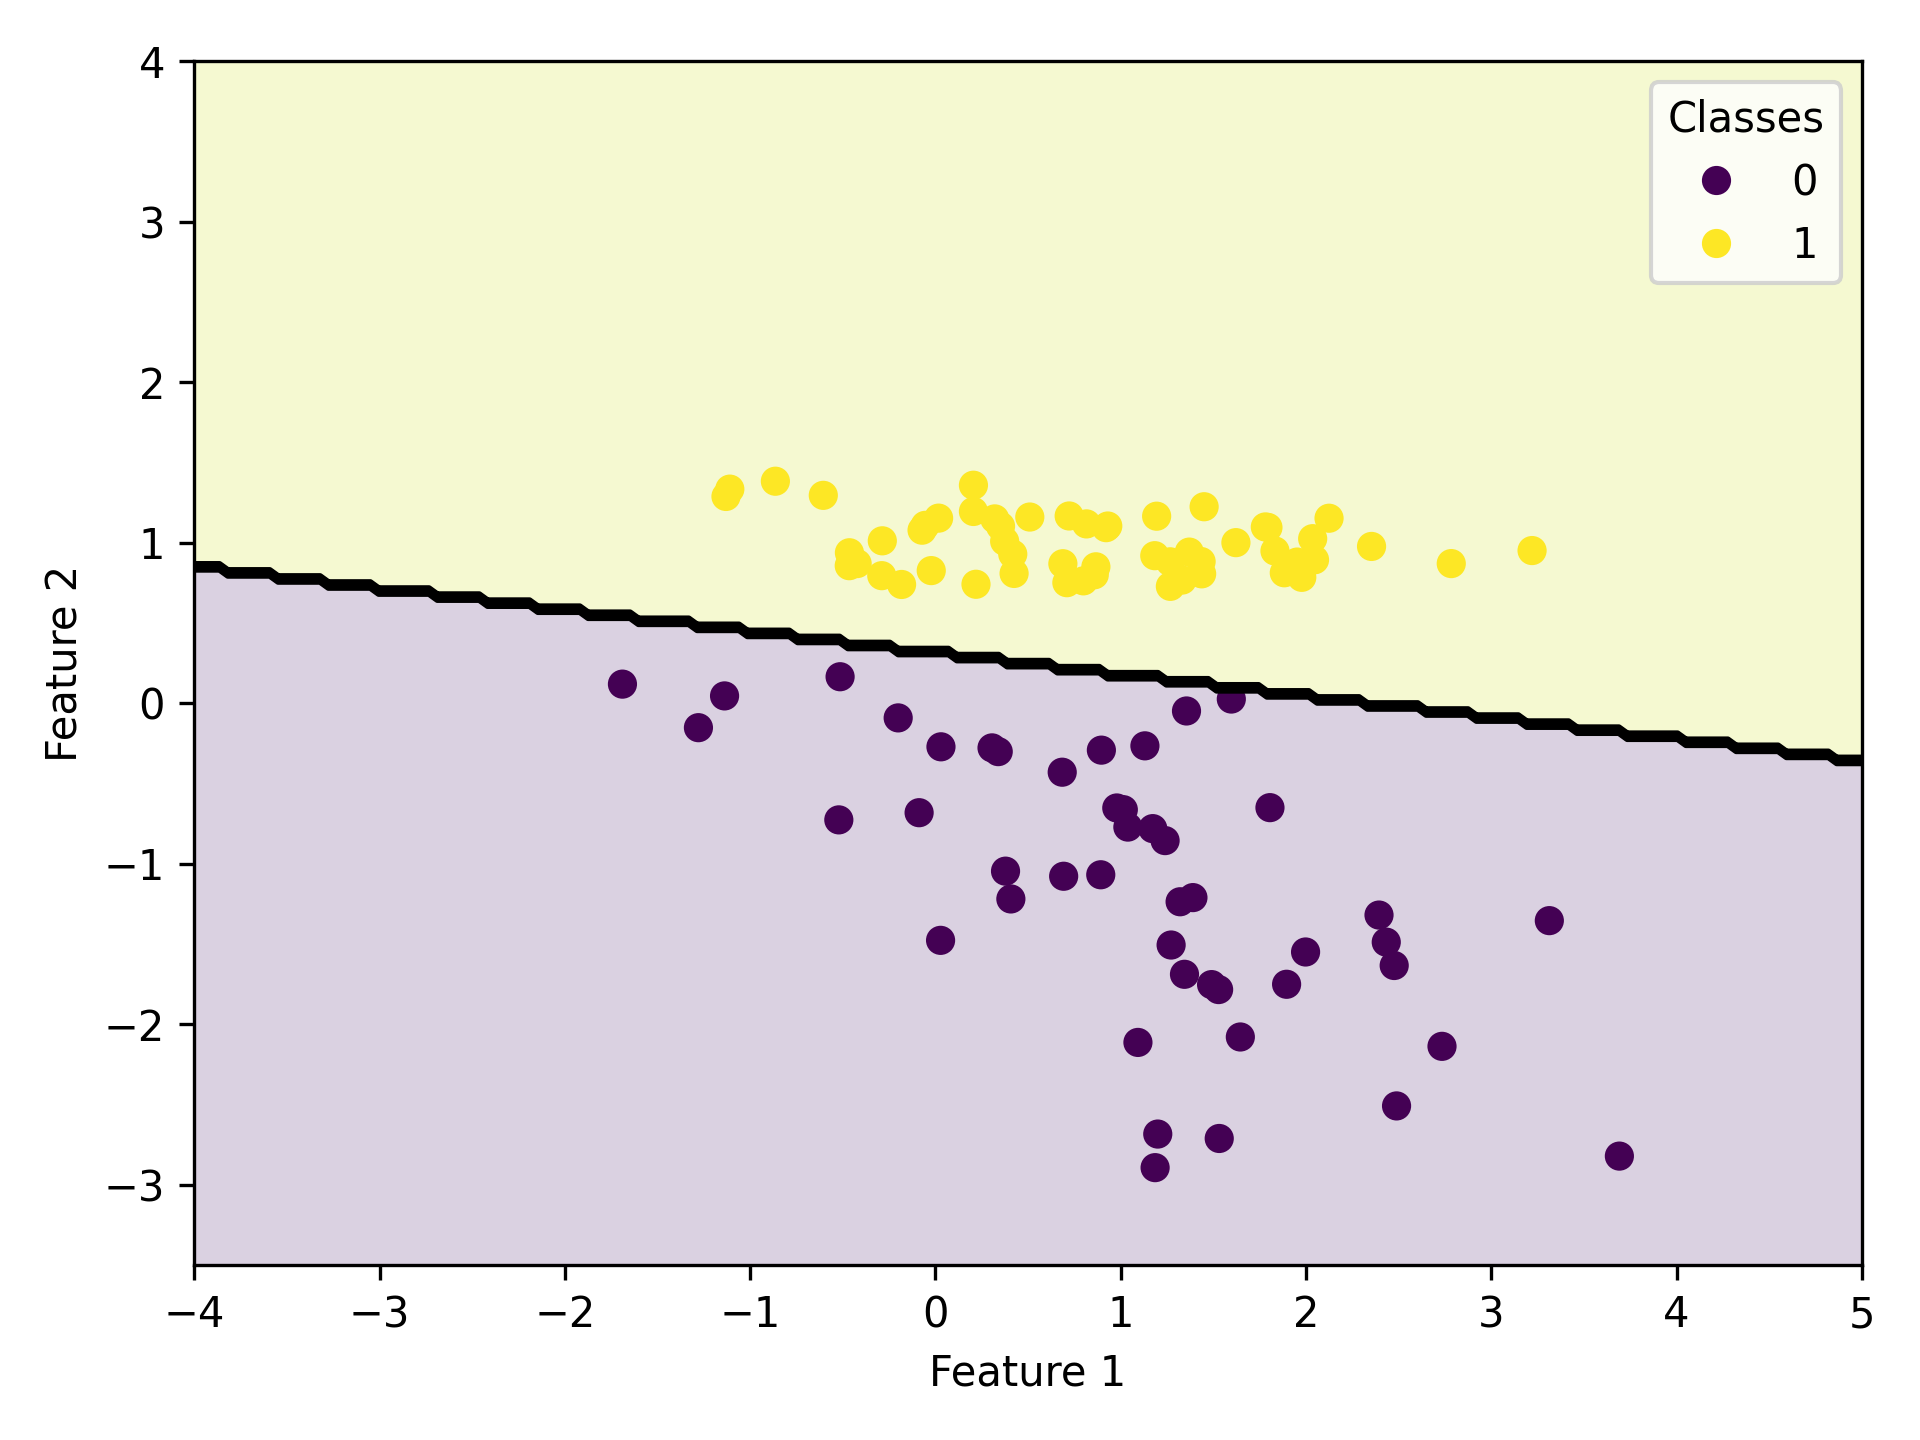
\includegraphics[width=\linewidth]{scatter_predictions_with_contour_3_learning_rate_349000000_sample_1000.png}
    \caption{$\alpha = 34.9$; $S = 1000$.}
  \end{subfigure}
  \hfill
  \begin{subfigure}[t]{0.24\textwidth}
    \centering
    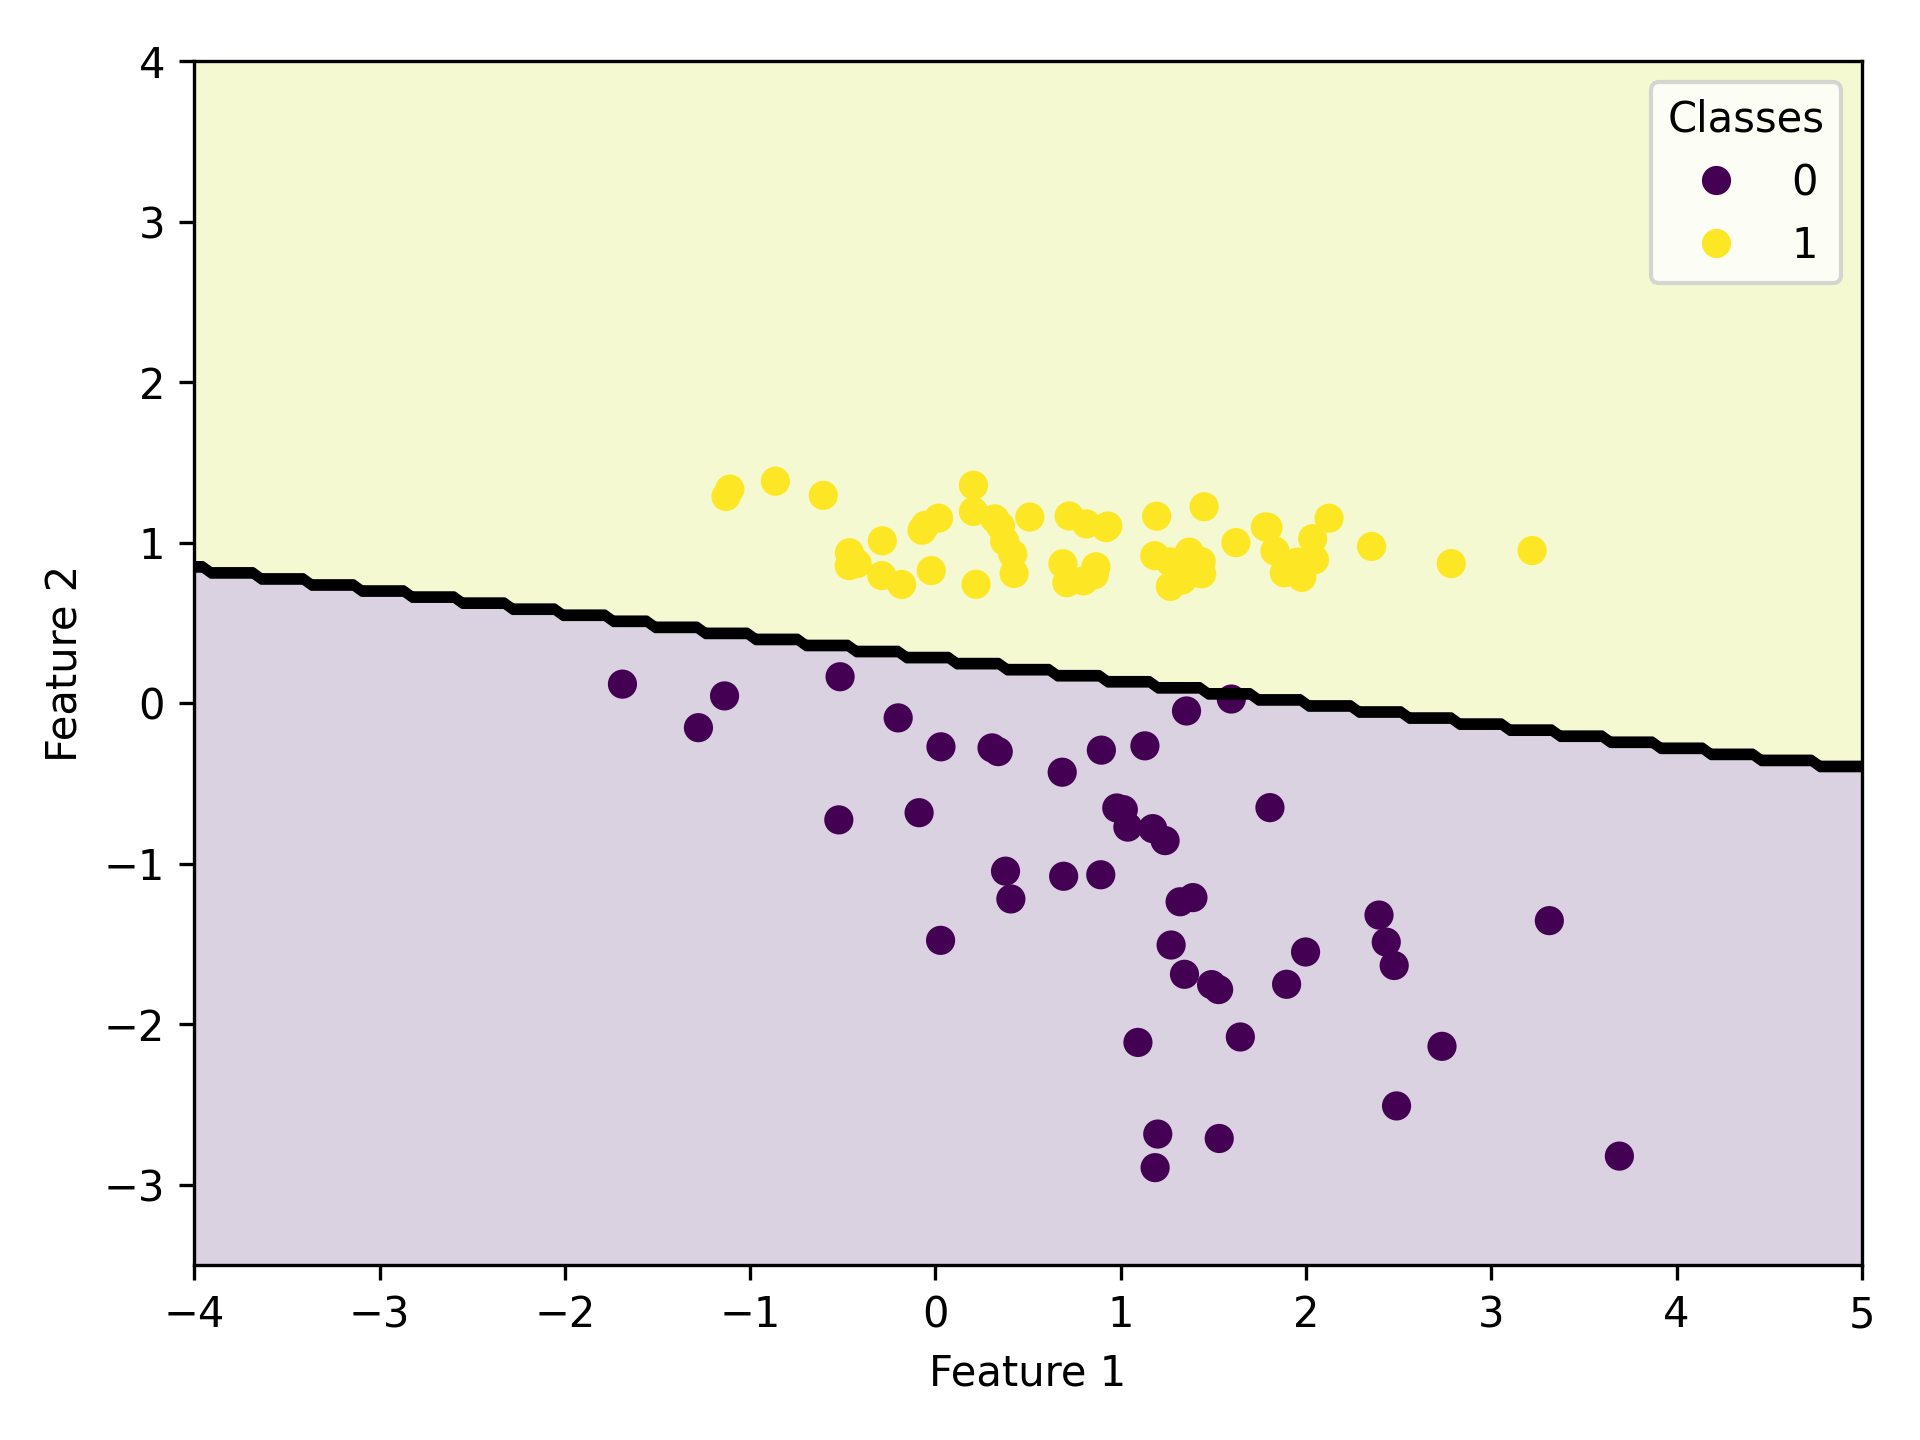
\includegraphics[width=\linewidth]{scatter_predictions_with_contour_3_learning_rate_349000000_sample_10000.png}
    \caption{$\alpha = 34.9$; $S = 10000$.}
  \end{subfigure}
  \hfill
  \begin{subfigure}[t]{0.24\textwidth}
    \centering
    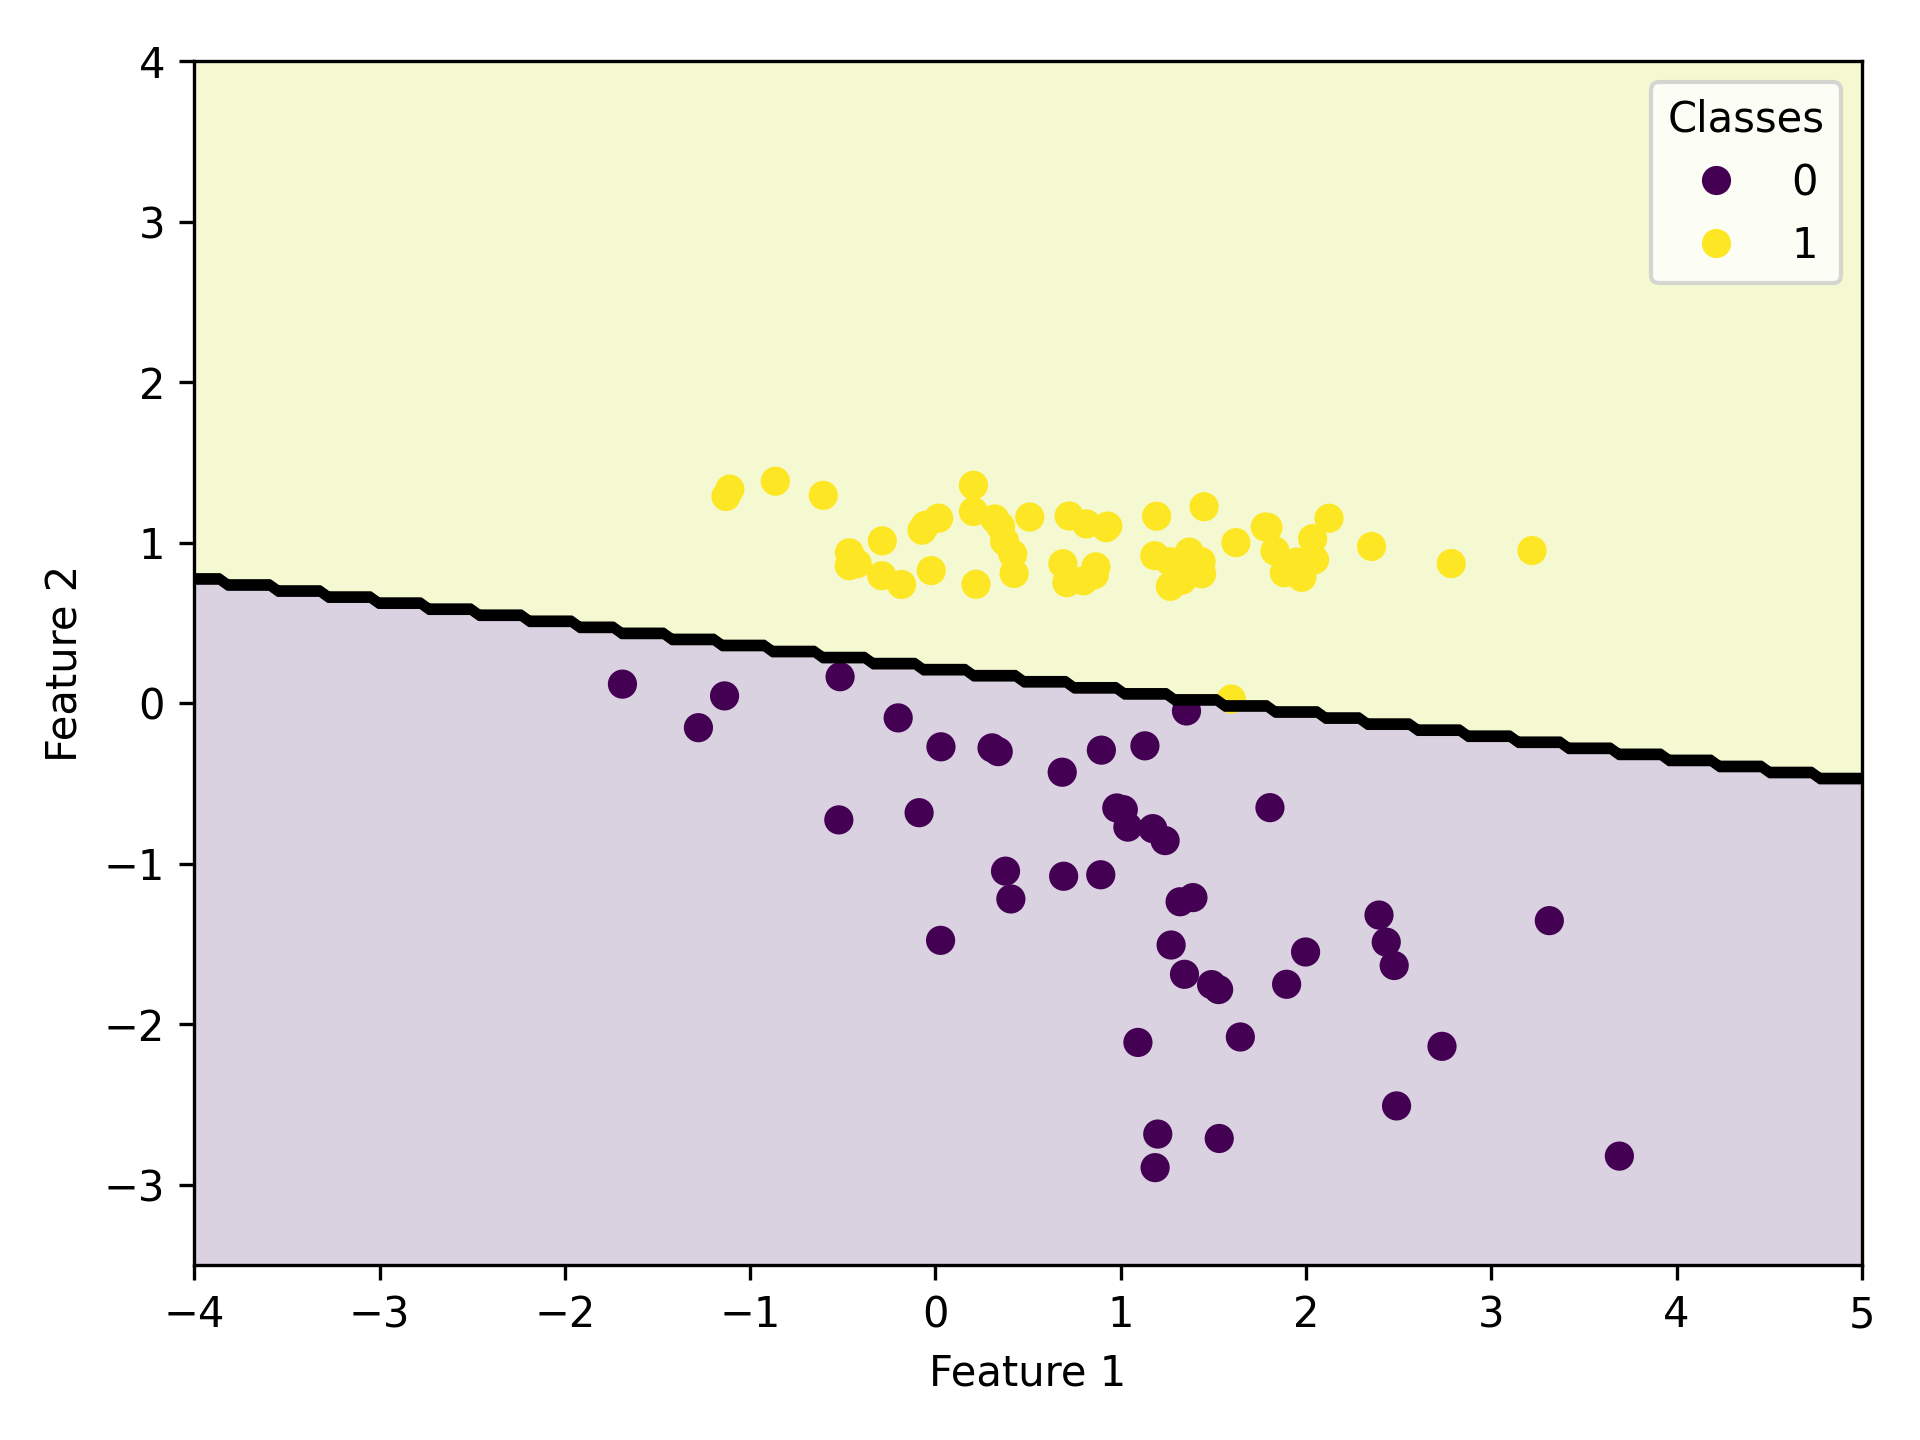
\includegraphics[width=\linewidth]{scatter_predictions_with_contour_3_learning_rate_349000000_sample_100000.png}
    \caption{$\alpha = 34.9$; $S = 100000$.}
  \end{subfigure}
  \caption{Scatter plot of the predictions over the test set with a linear boundary decision, using different learning rates ($\alpha$) and sample sizes ($S$) for Monte Carlo approximation.}
  \label{fig:discriminative_results}
\end{figure}

% Histogram - W bias
\begin{figure}
  \centering
  \begin{subfigure}[t]{0.24\textwidth}
    \centering
    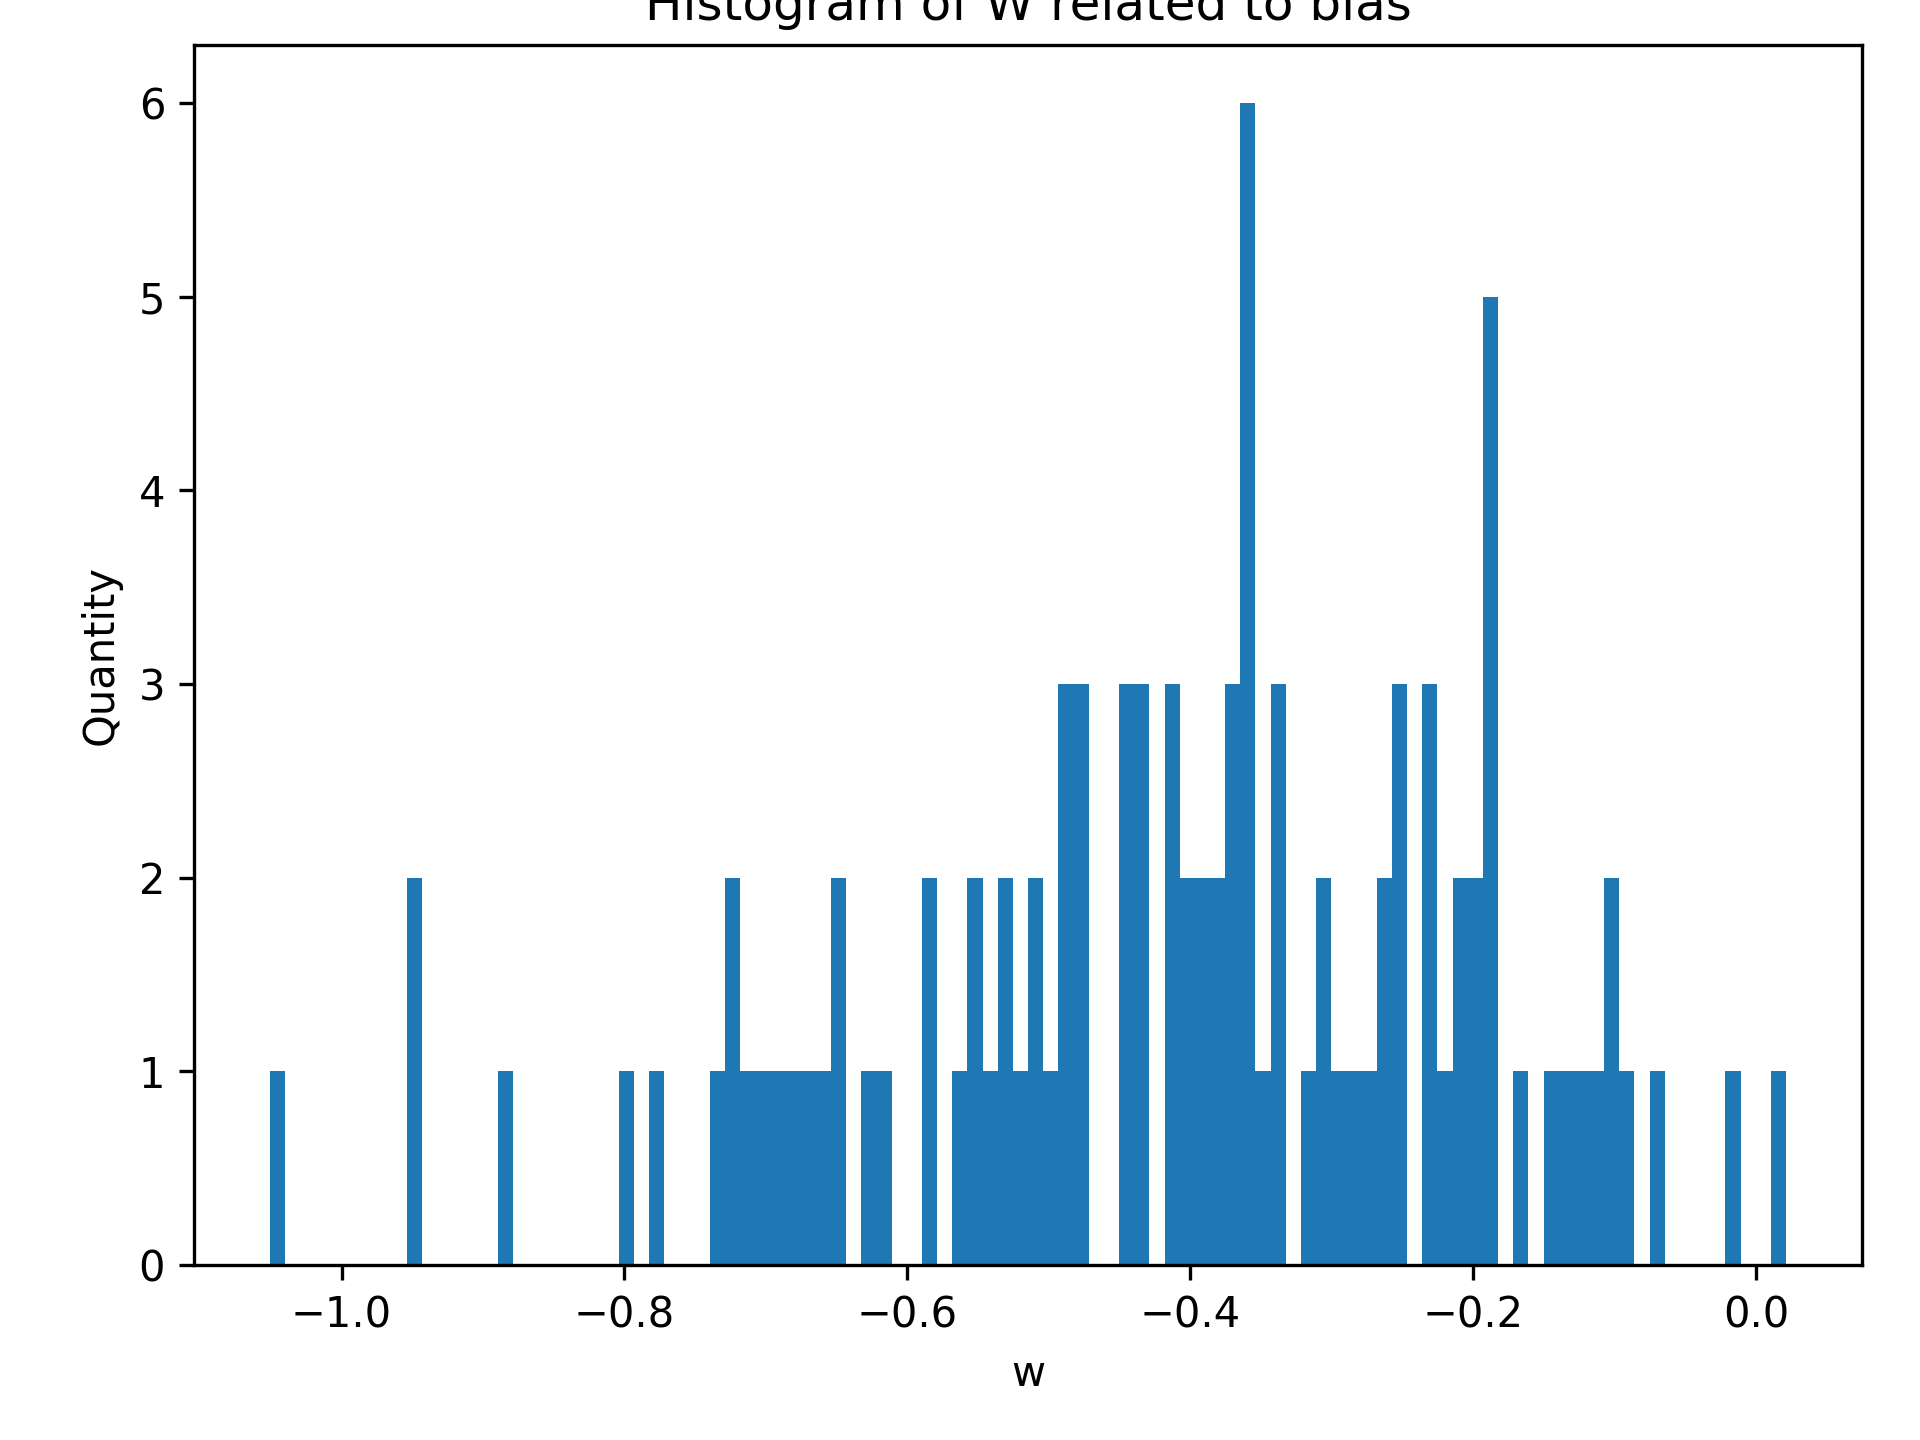
\includegraphics[width=\linewidth]{hist_featbias_1_sample_100.png}
    \caption{$\alpha = 1e-7$; $S = 100$.}
  \end{subfigure}
  \hfill
  \begin{subfigure}[t]{0.24\textwidth}
    \centering
    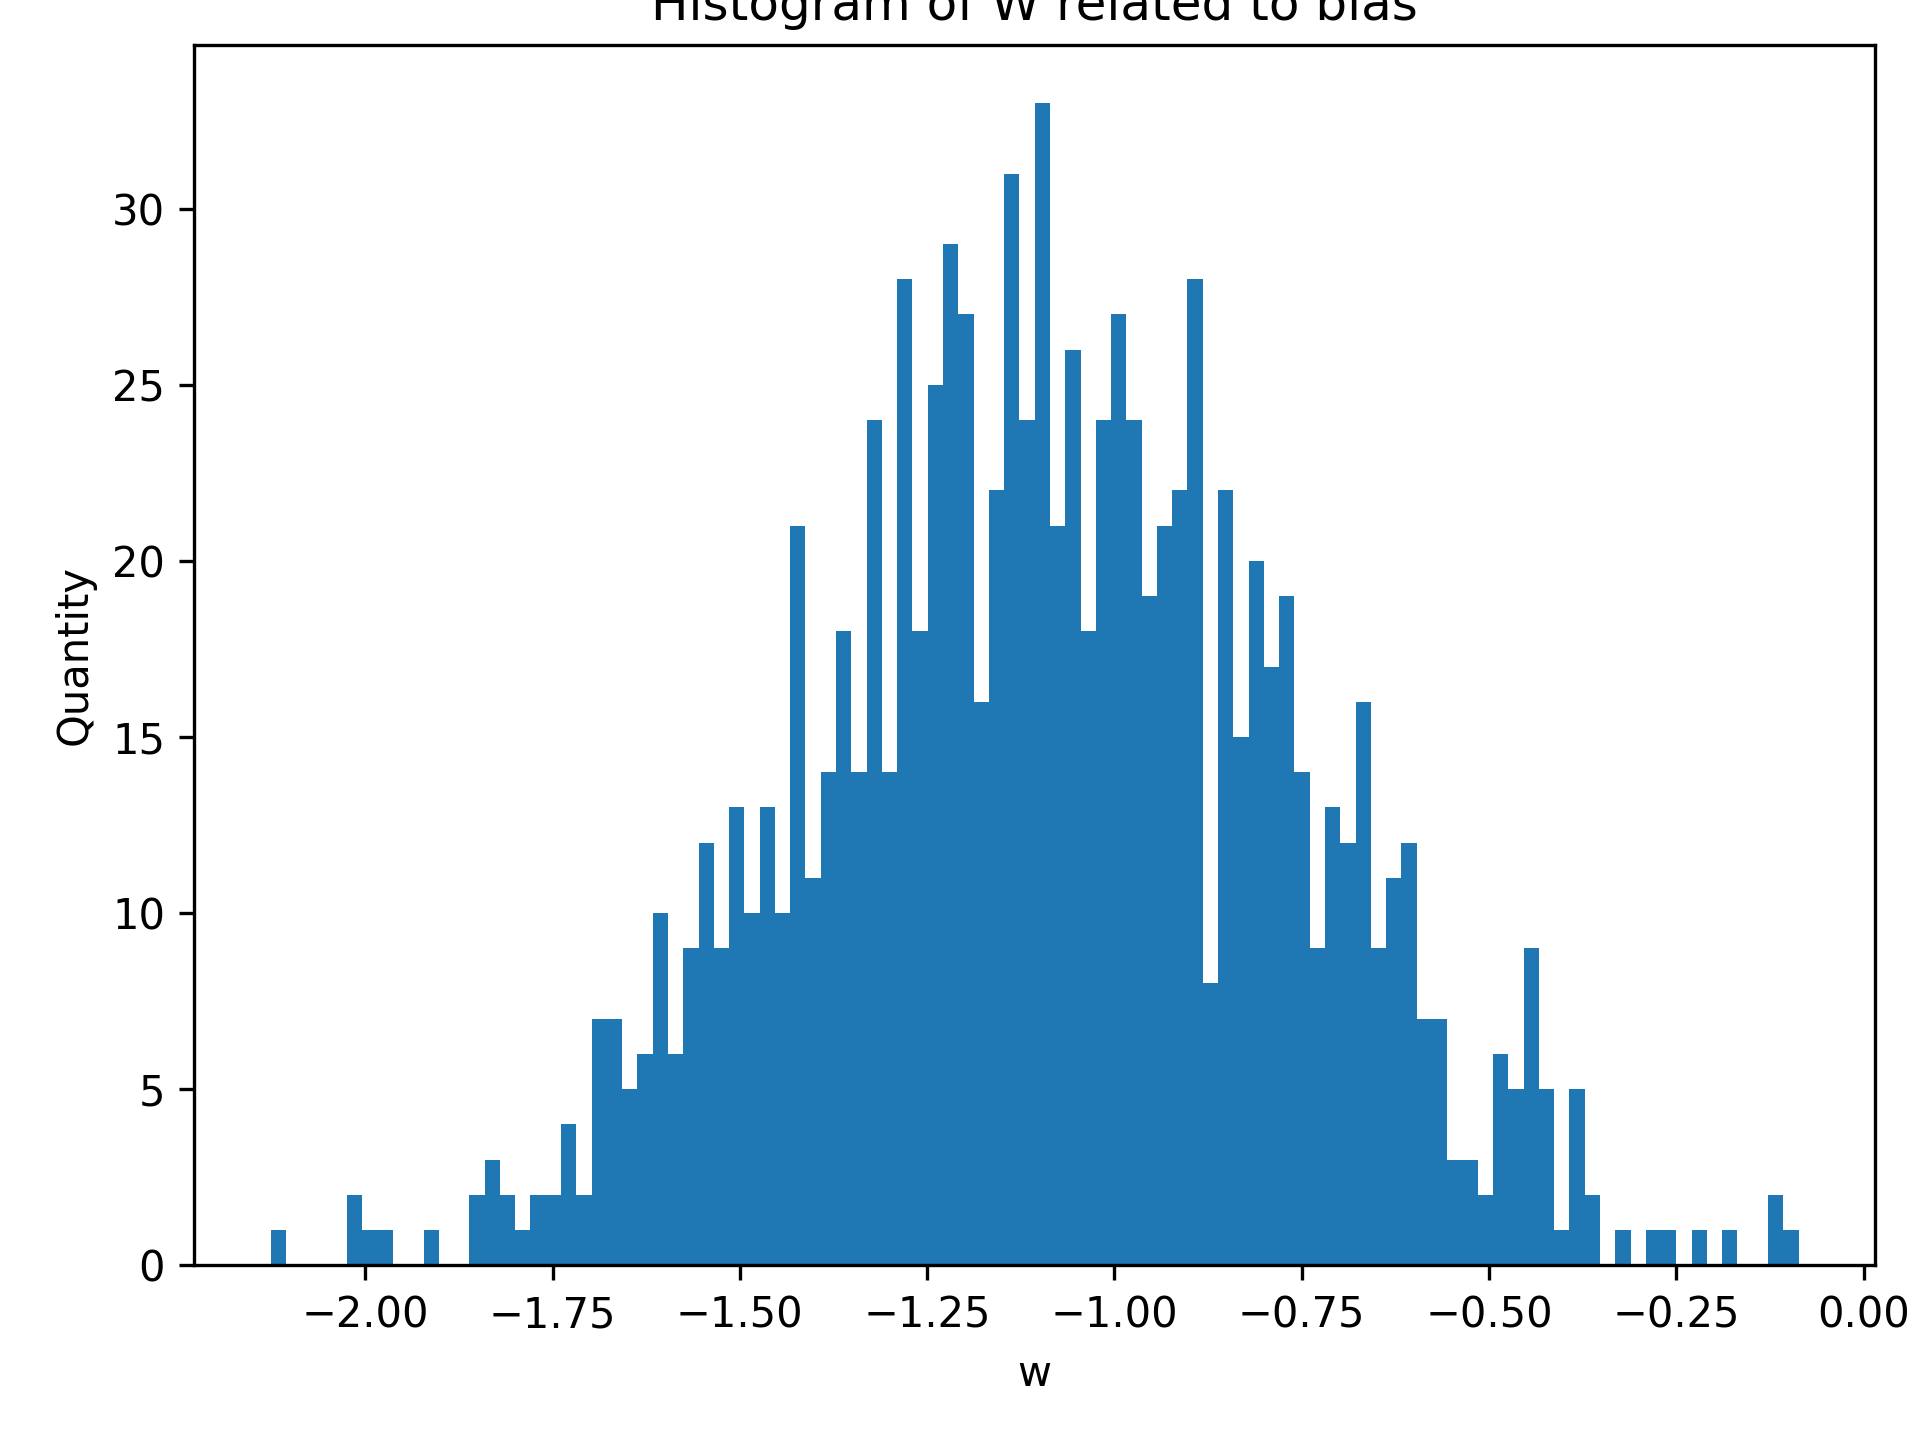
\includegraphics[width=\linewidth]{hist_featbias_1_sample_1000.png}
    \caption{$\alpha = 1e-7$; $S = 1000$.}
  \end{subfigure}
  \hfill
  \begin{subfigure}[t]{0.24\textwidth}
    \centering
    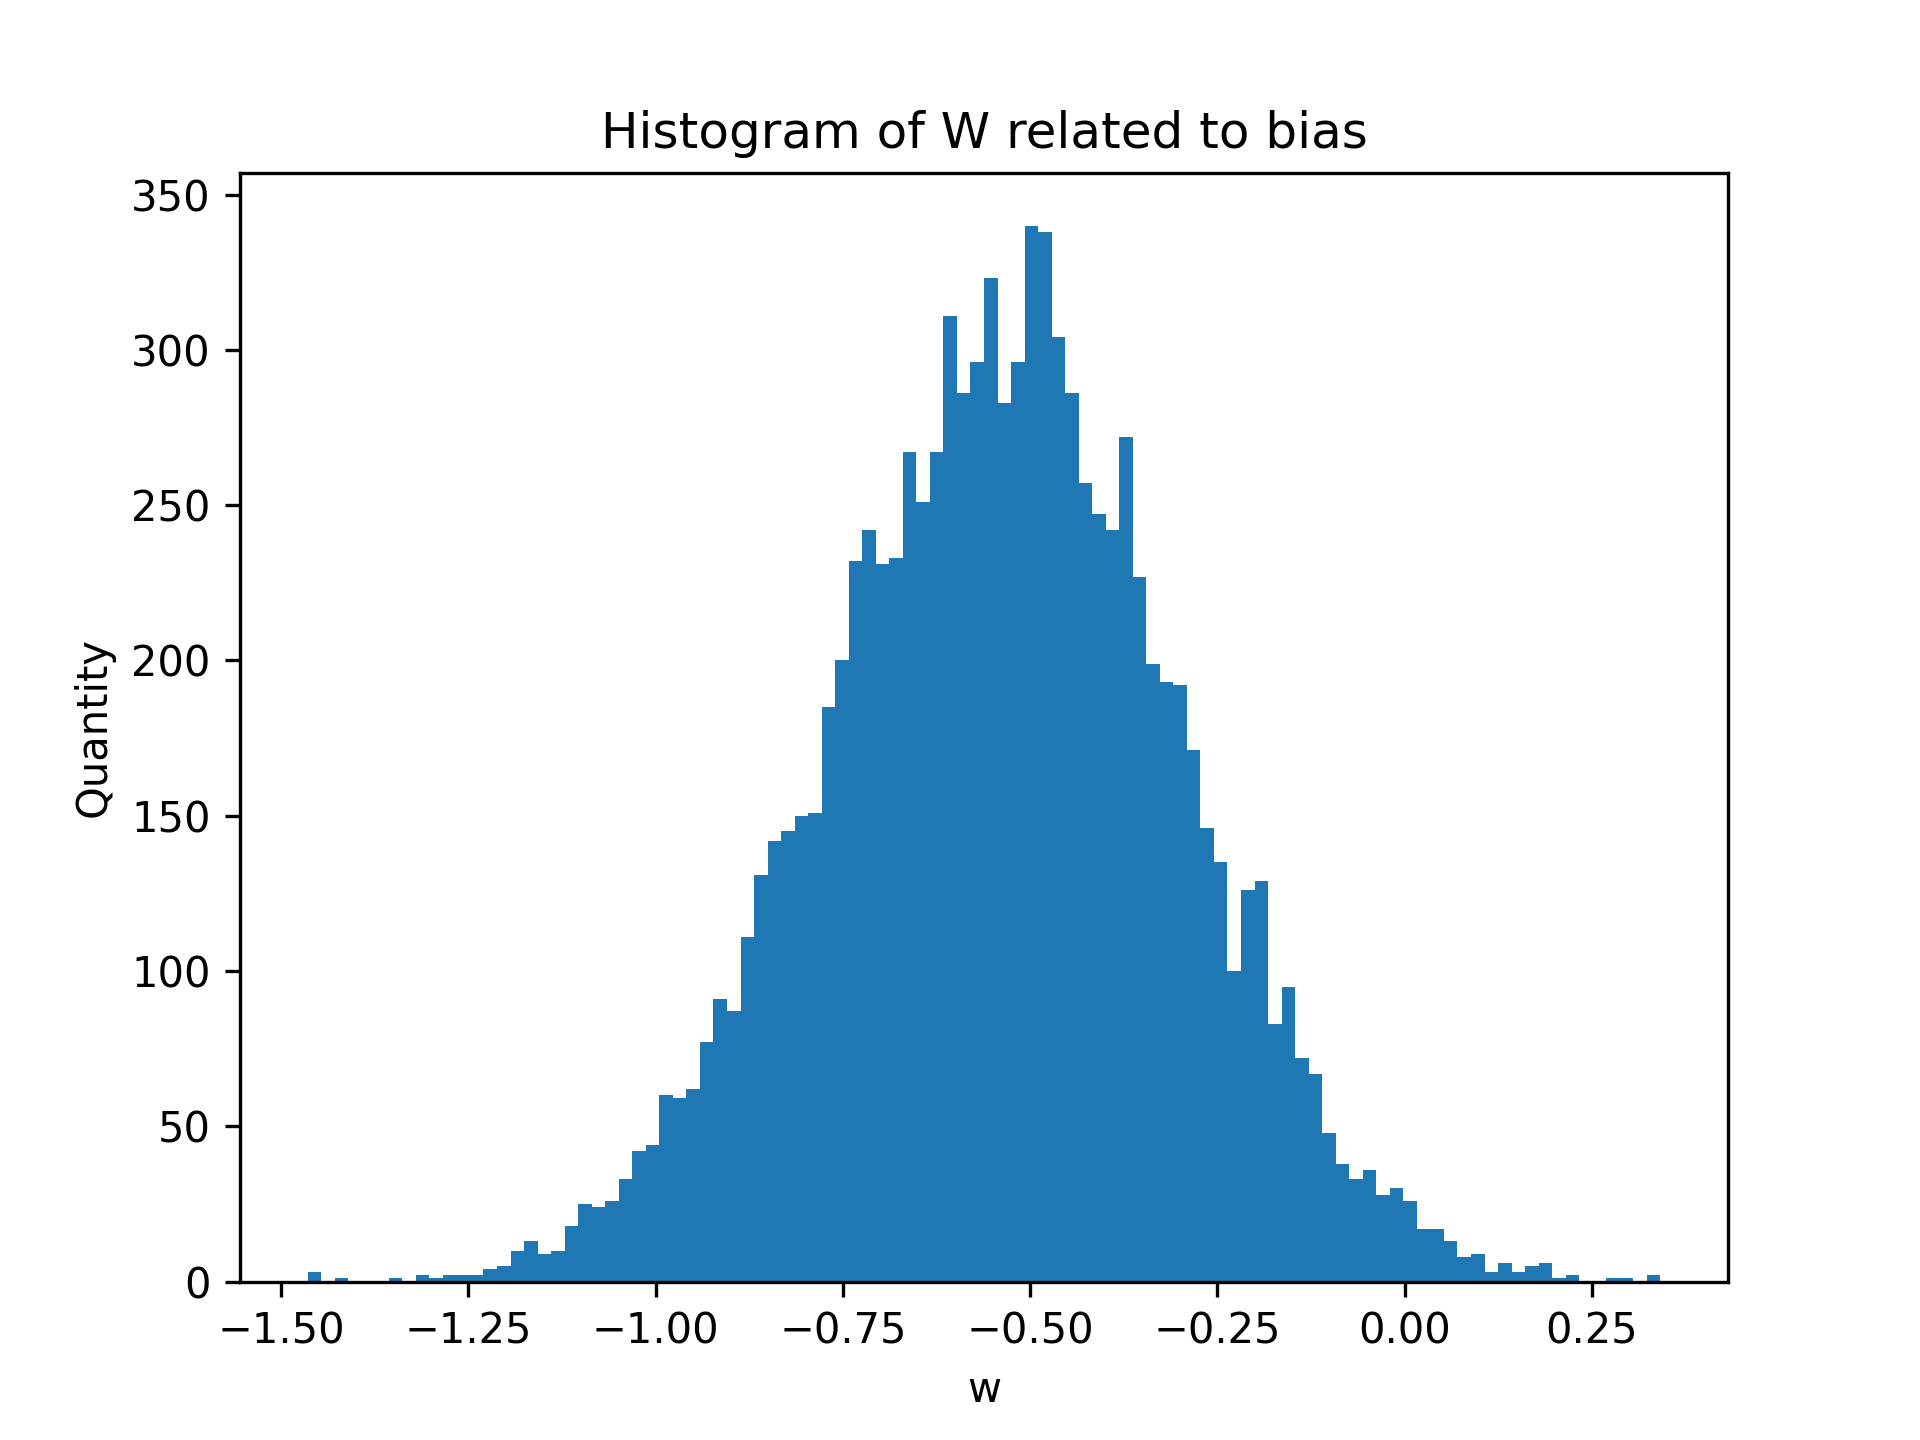
\includegraphics[width=\linewidth]{hist_featbias_1_sample_10000.png}
    \caption{$\alpha = 1e-7$; $S = 10000$.}
  \end{subfigure}
  \hfill
  \begin{subfigure}[t]{0.24\textwidth}
    \centering
    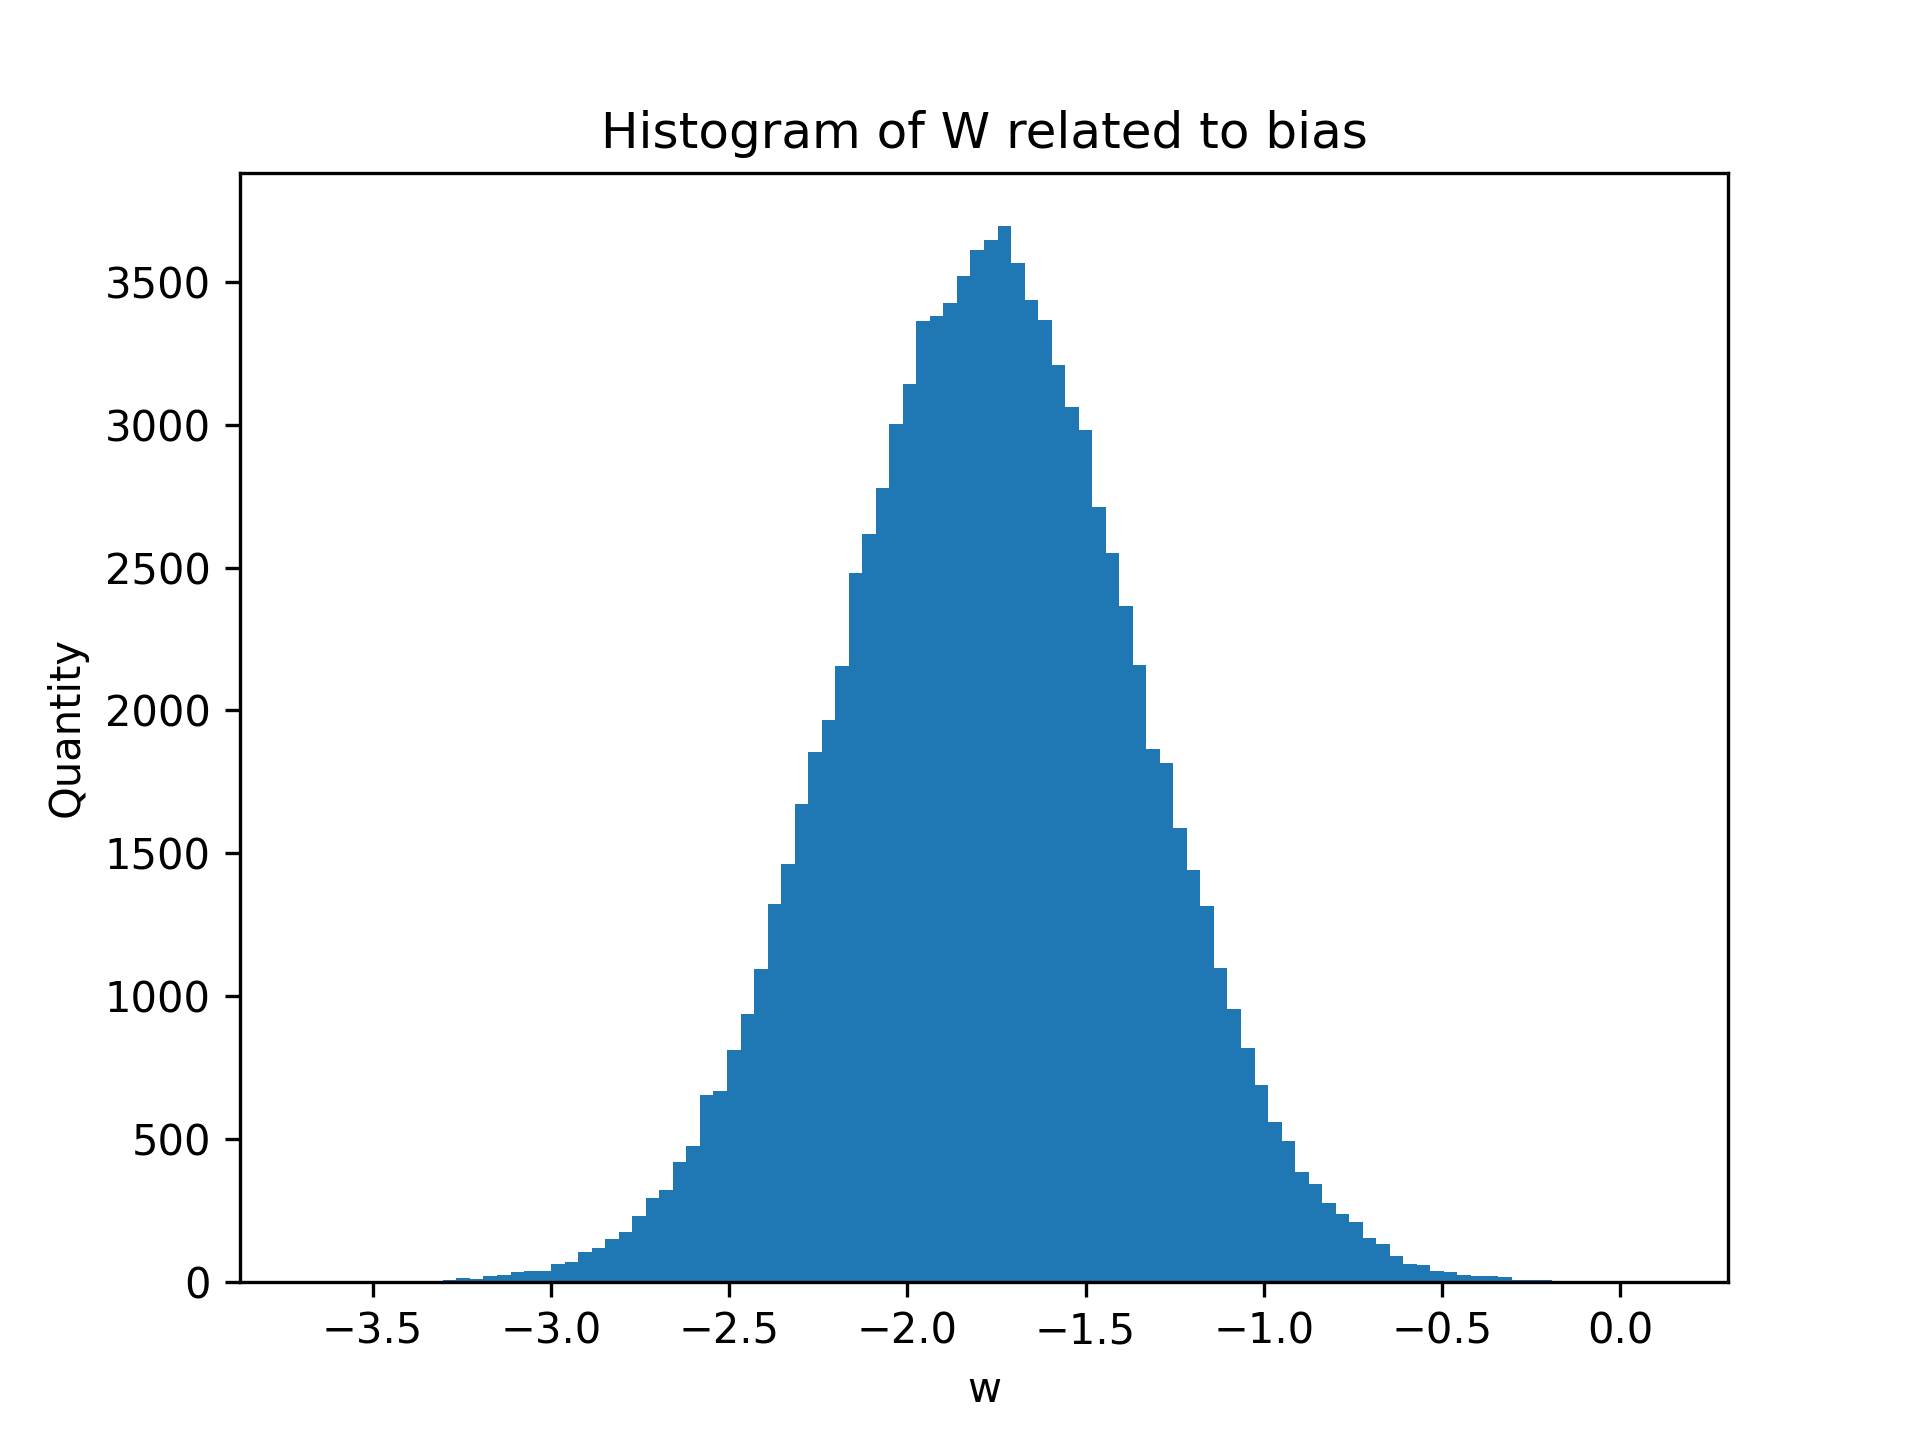
\includegraphics[width=\linewidth]{hist_featbias_1_sample_100000.png}
    \caption{$\alpha = 1e-7$; $S = 100000$.}
  \end{subfigure}
  % \hfill
  \begin{subfigure}[t]{0.24\textwidth}
    \centering
    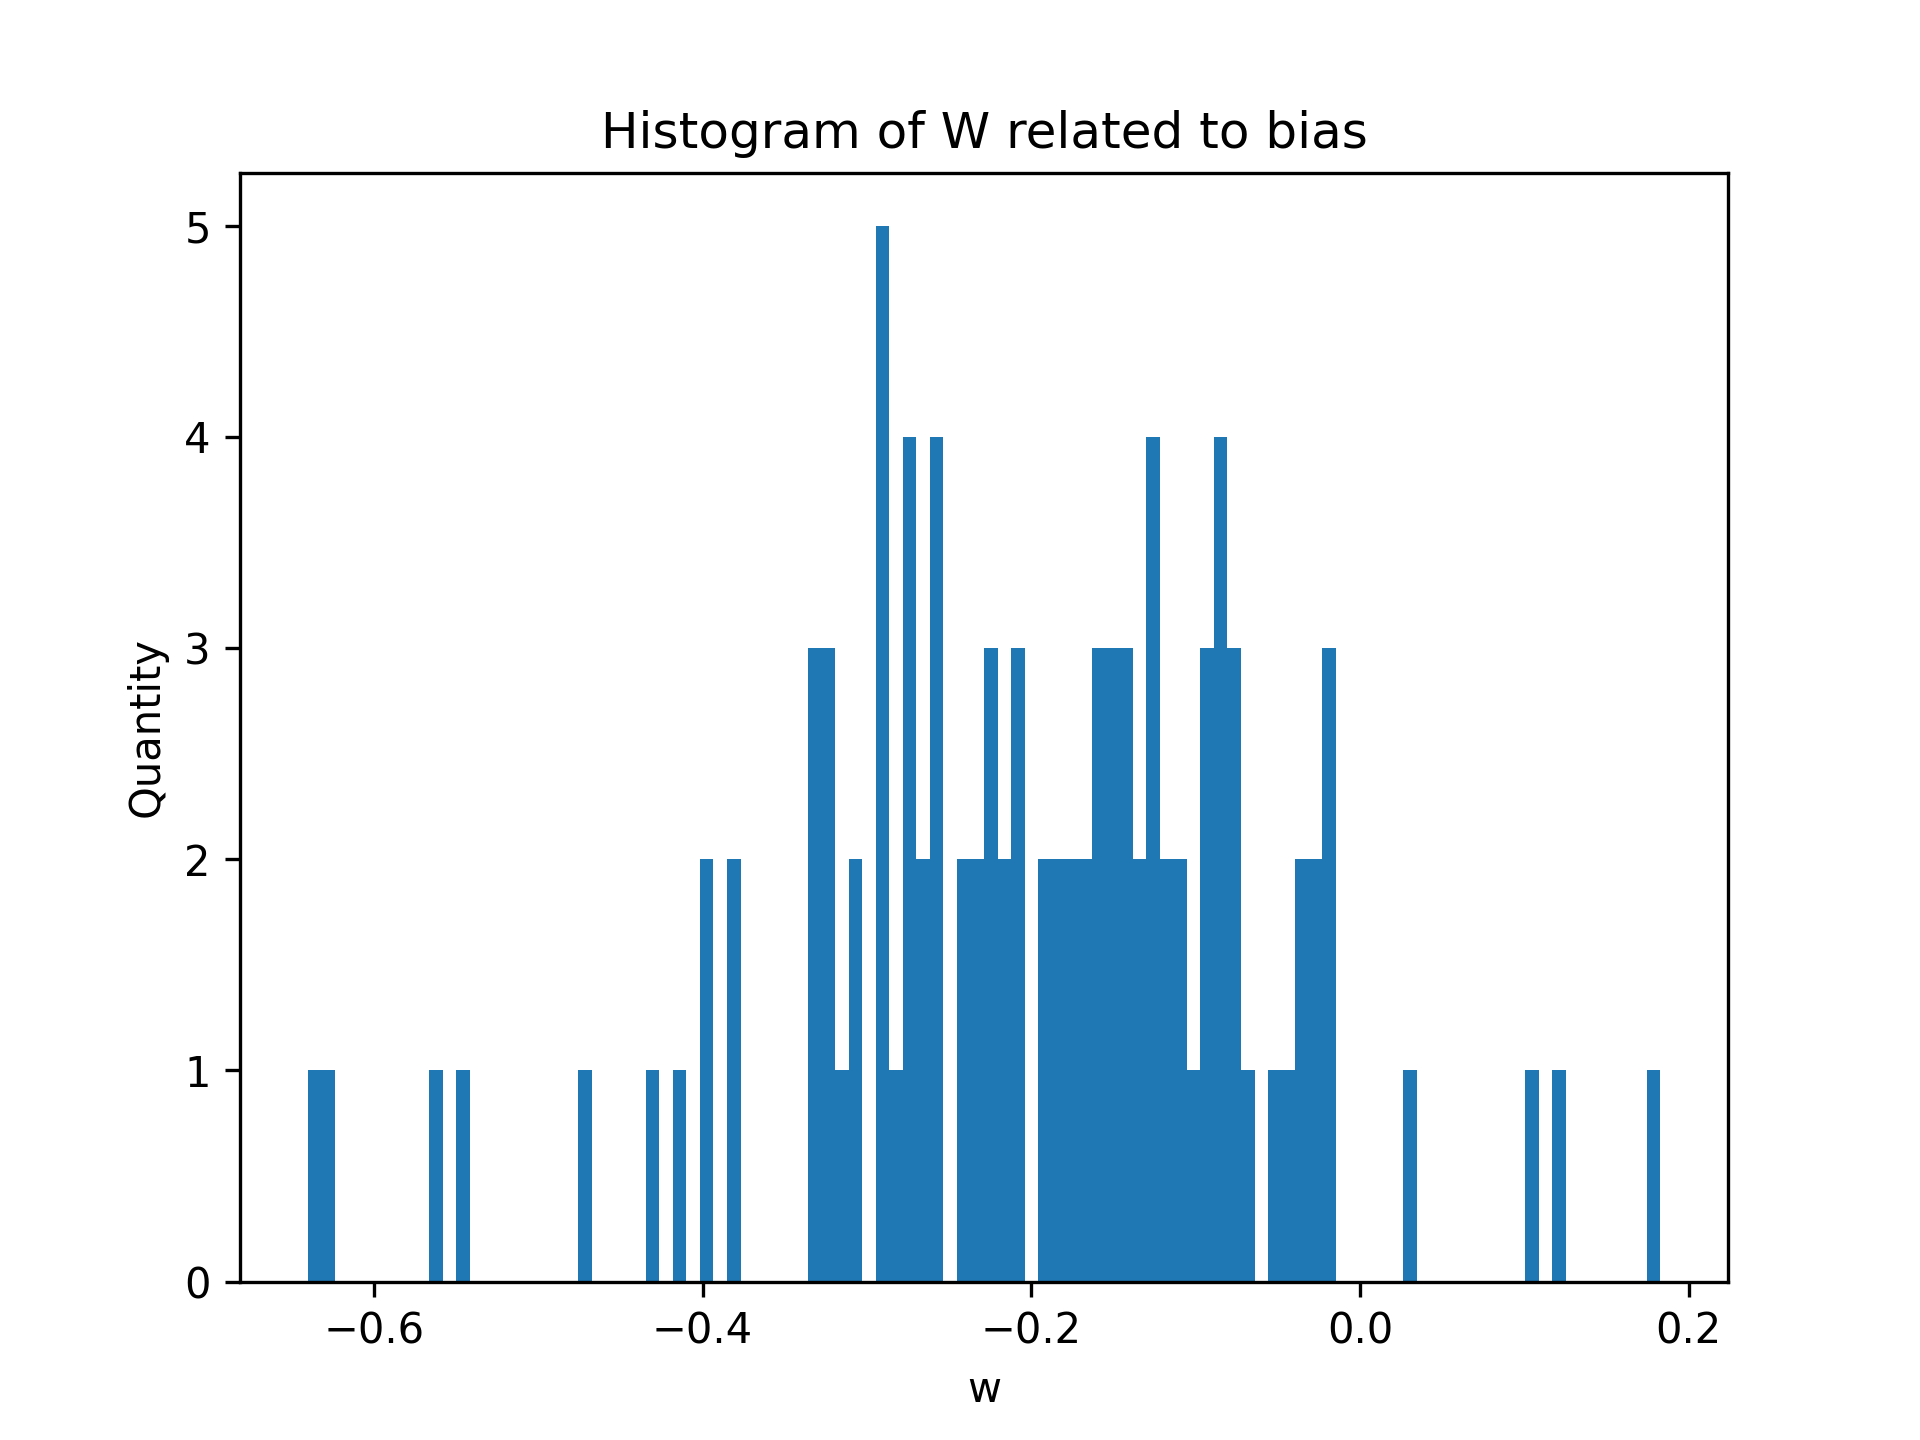
\includegraphics[width=\linewidth]{hist_featbias_10000_sample_100.png}
    \caption{$\alpha = 1e-3$; $S = 100$.}
  \end{subfigure}
  \hfill
  \begin{subfigure}[t]{0.24\textwidth}
    \centering
    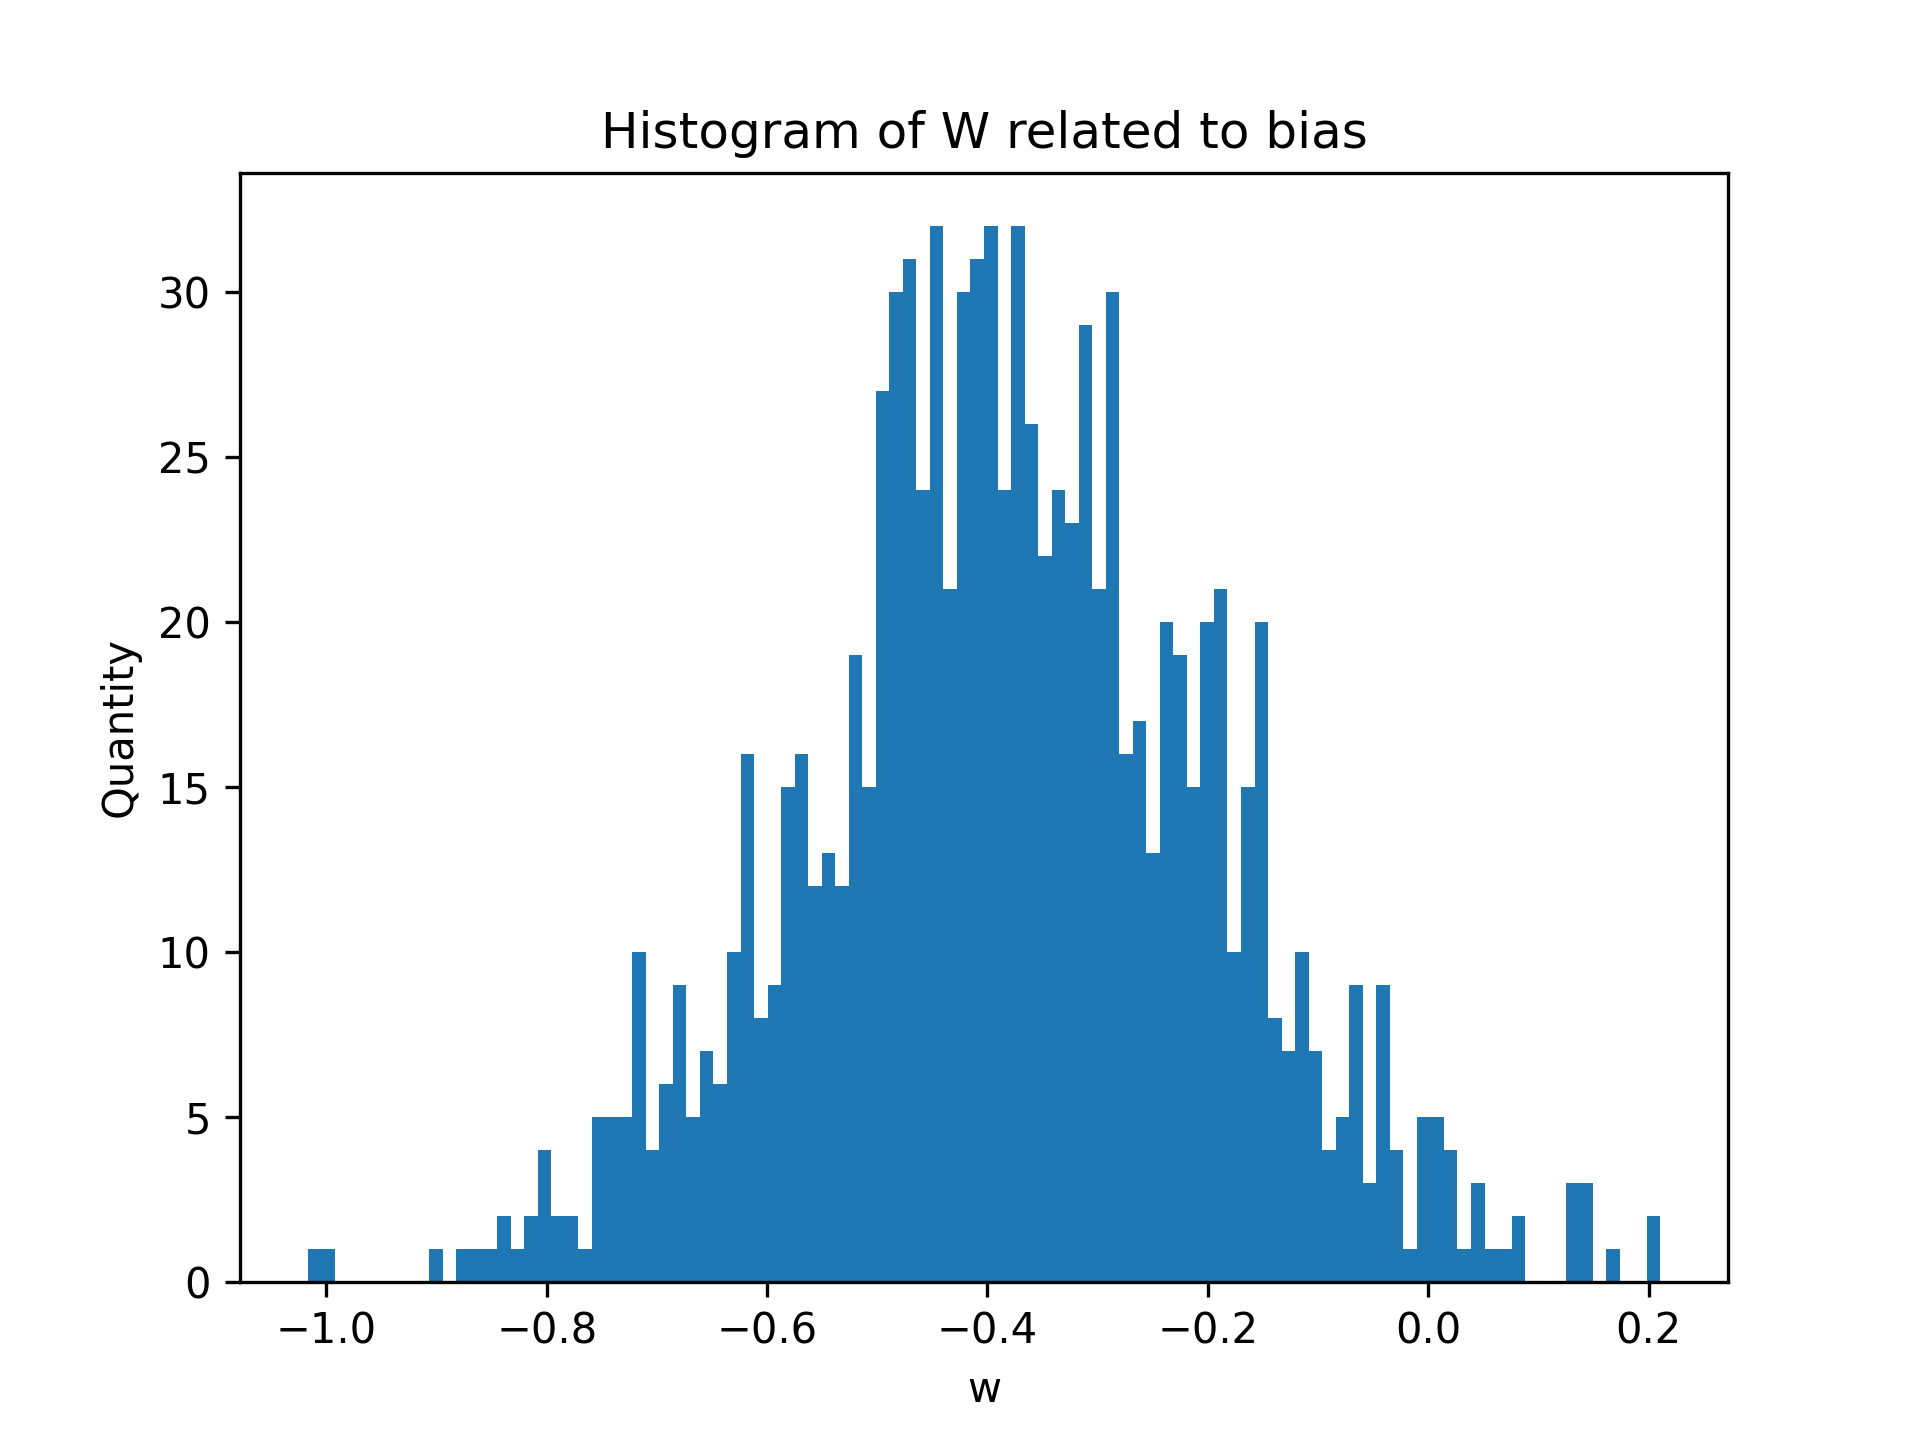
\includegraphics[width=\linewidth]{hist_featbias_10000_sample_1000.png}
    \caption{$\alpha = 1e-3$; $S = 1000$.}
  \end{subfigure}
  \hfill
  \begin{subfigure}[t]{0.24\textwidth}
    \centering
    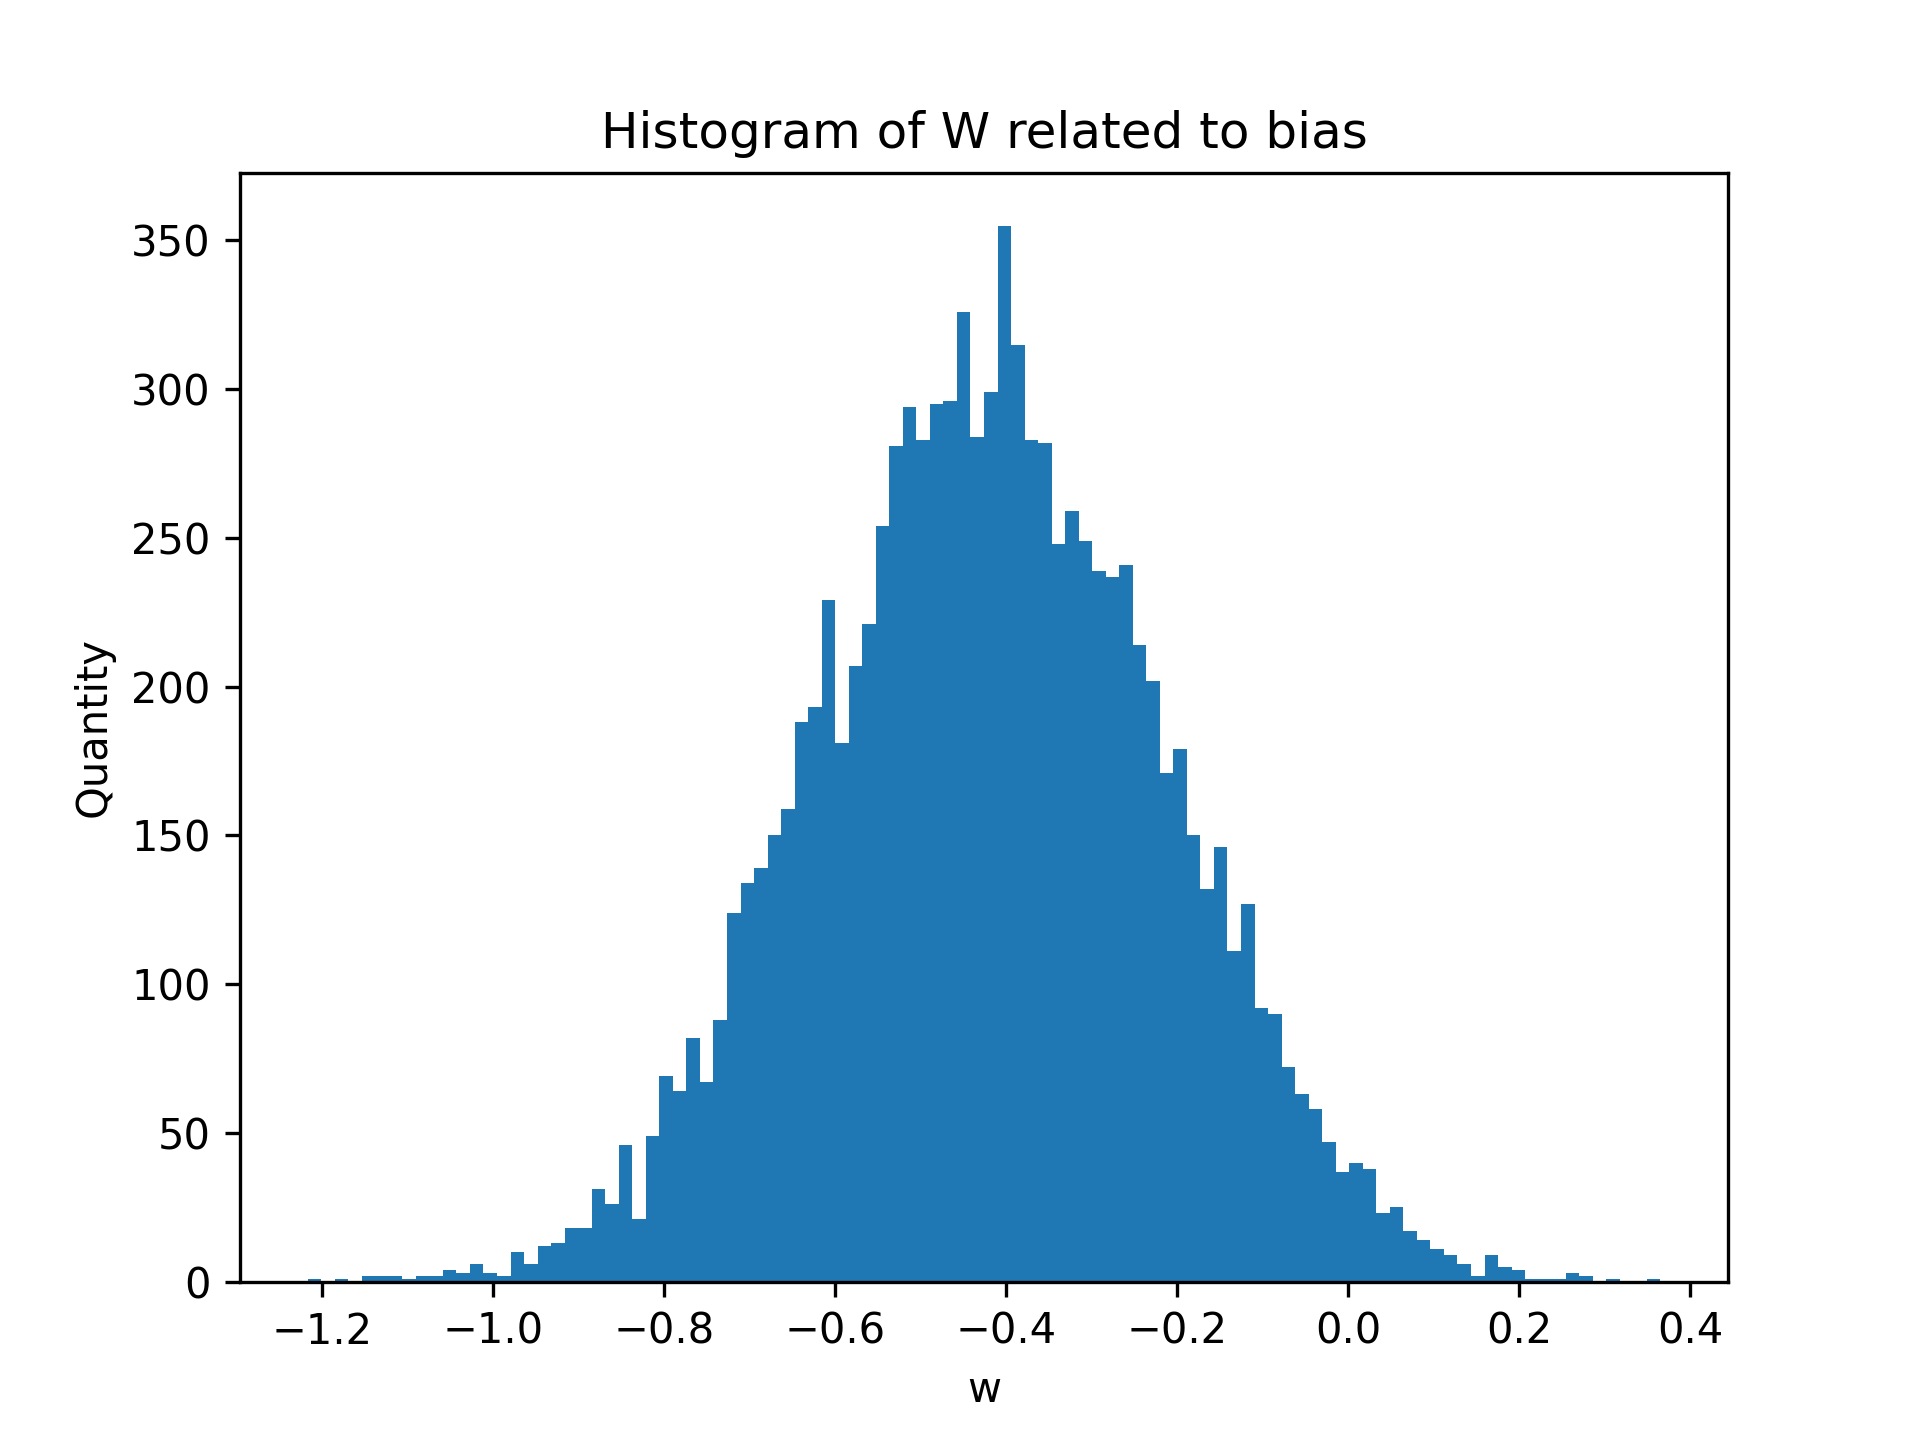
\includegraphics[width=\linewidth]{hist_featbias_10000_sample_10000.png}
    \caption{$\alpha = 1e-3$; $S = 10000$.}
  \end{subfigure}
  \hfill
  \begin{subfigure}[t]{0.24\textwidth}
    \centering
    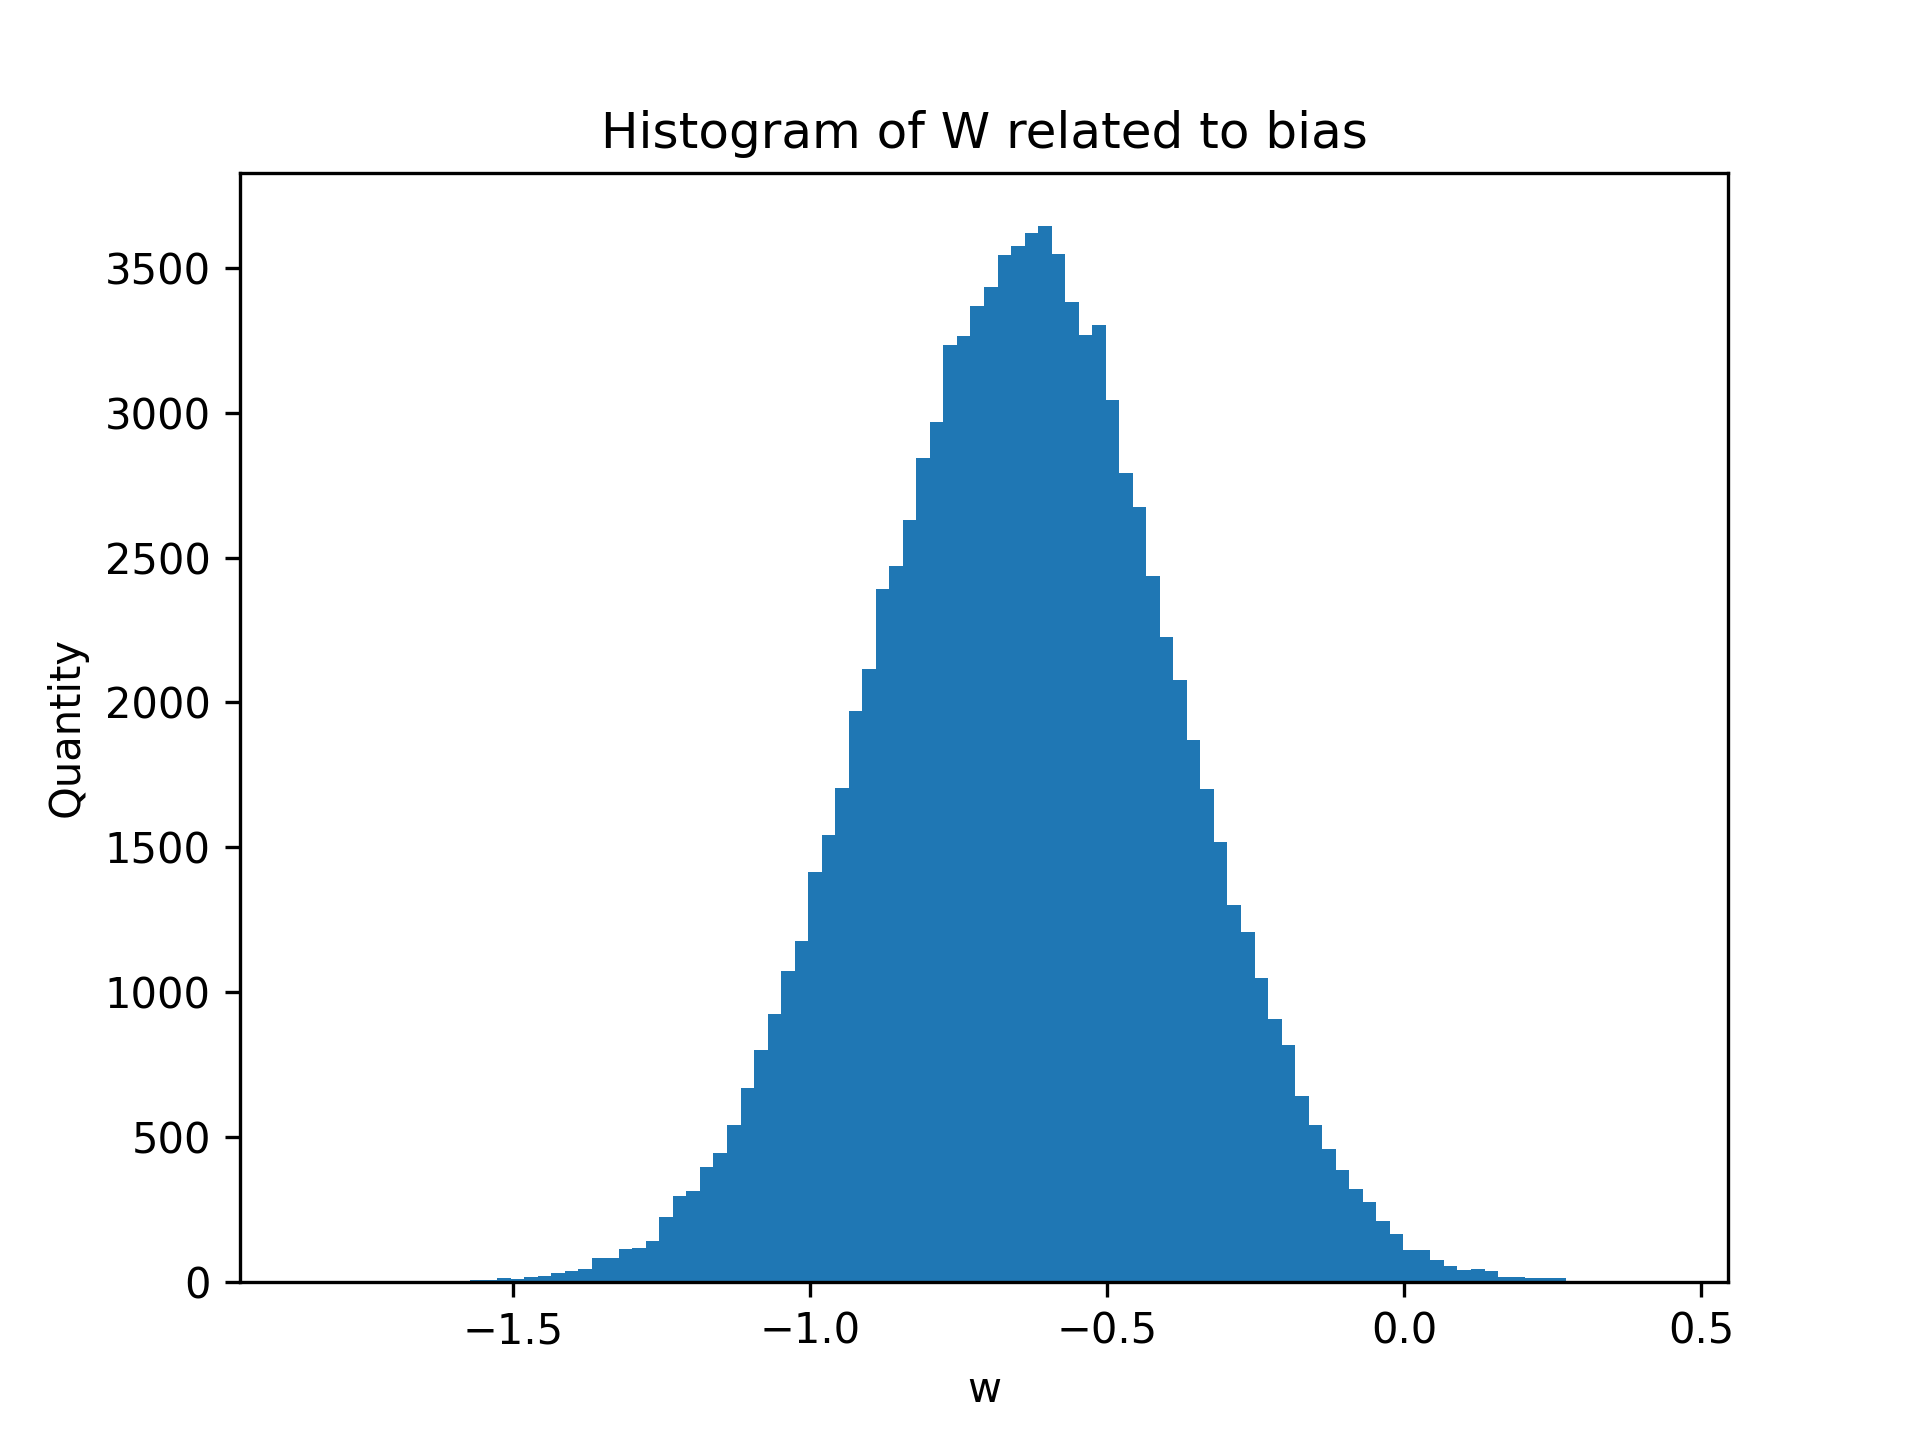
\includegraphics[width=\linewidth]{hist_featbias_10000_sample_100000.png}
    \caption{$\alpha = 1e-3$; $S = 100000$.}
  \end{subfigure}
  % \hfill
  \begin{subfigure}[t]{0.24\textwidth}
    \centering
    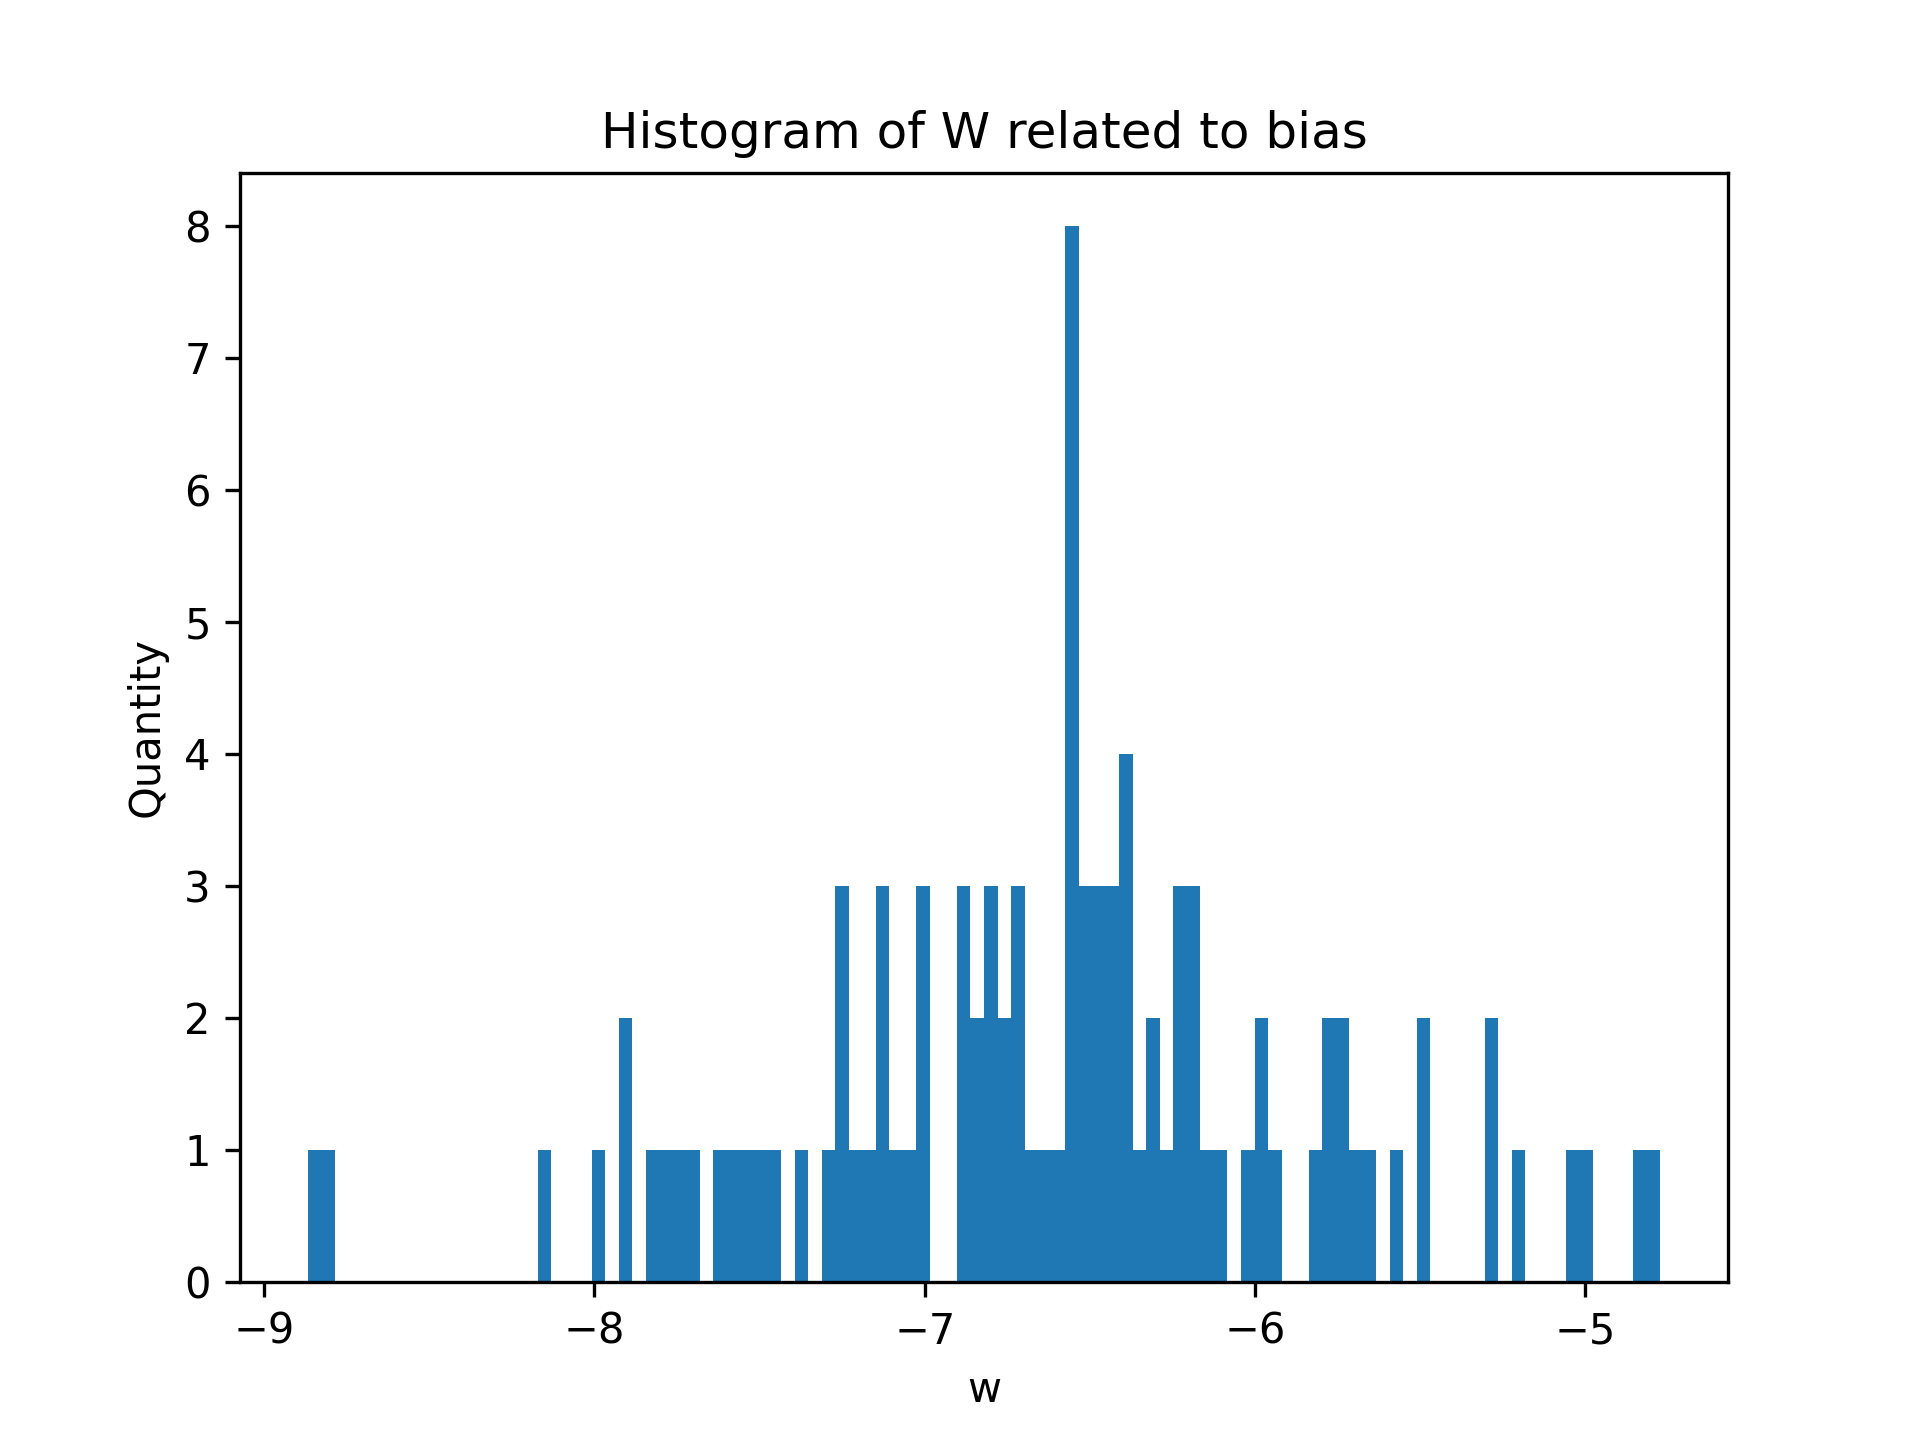
\includegraphics[width=\linewidth]{hist_featbias_349000000_sample_100.png}
    \caption{$\alpha = 34.9$; $S = 100$.}
  \end{subfigure}
  \hfill
  \begin{subfigure}[t]{0.24\textwidth}
    \centering
    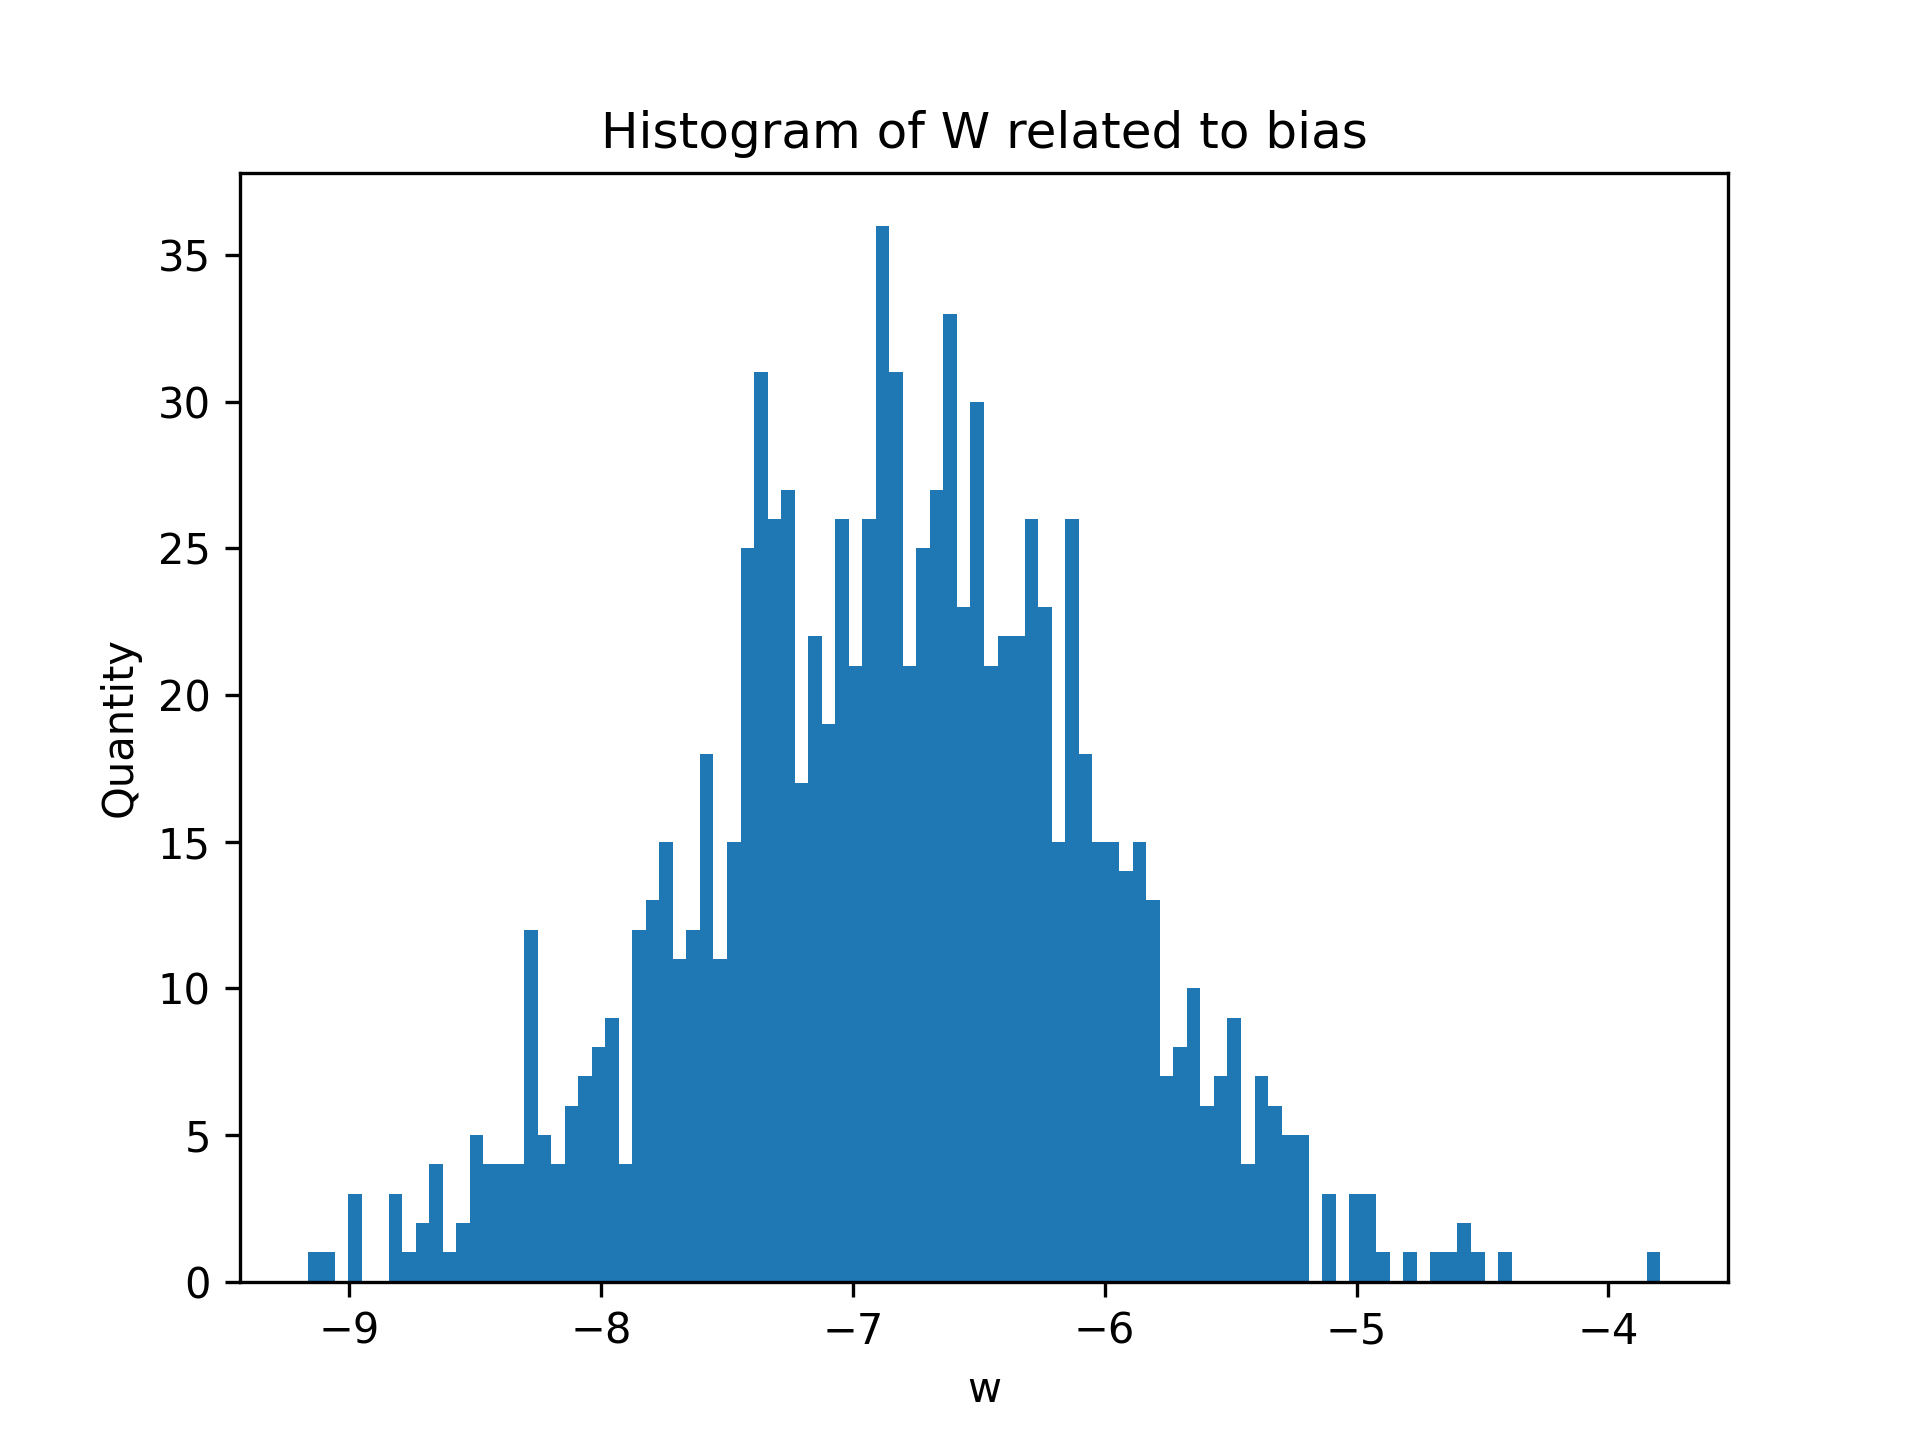
\includegraphics[width=\linewidth]{hist_featbias_349000000_sample_1000.png}
    \caption{$\alpha = 34.9$; $S = 1000$.}
  \end{subfigure}
  \hfill
  \begin{subfigure}[t]{0.24\textwidth}
    \centering
    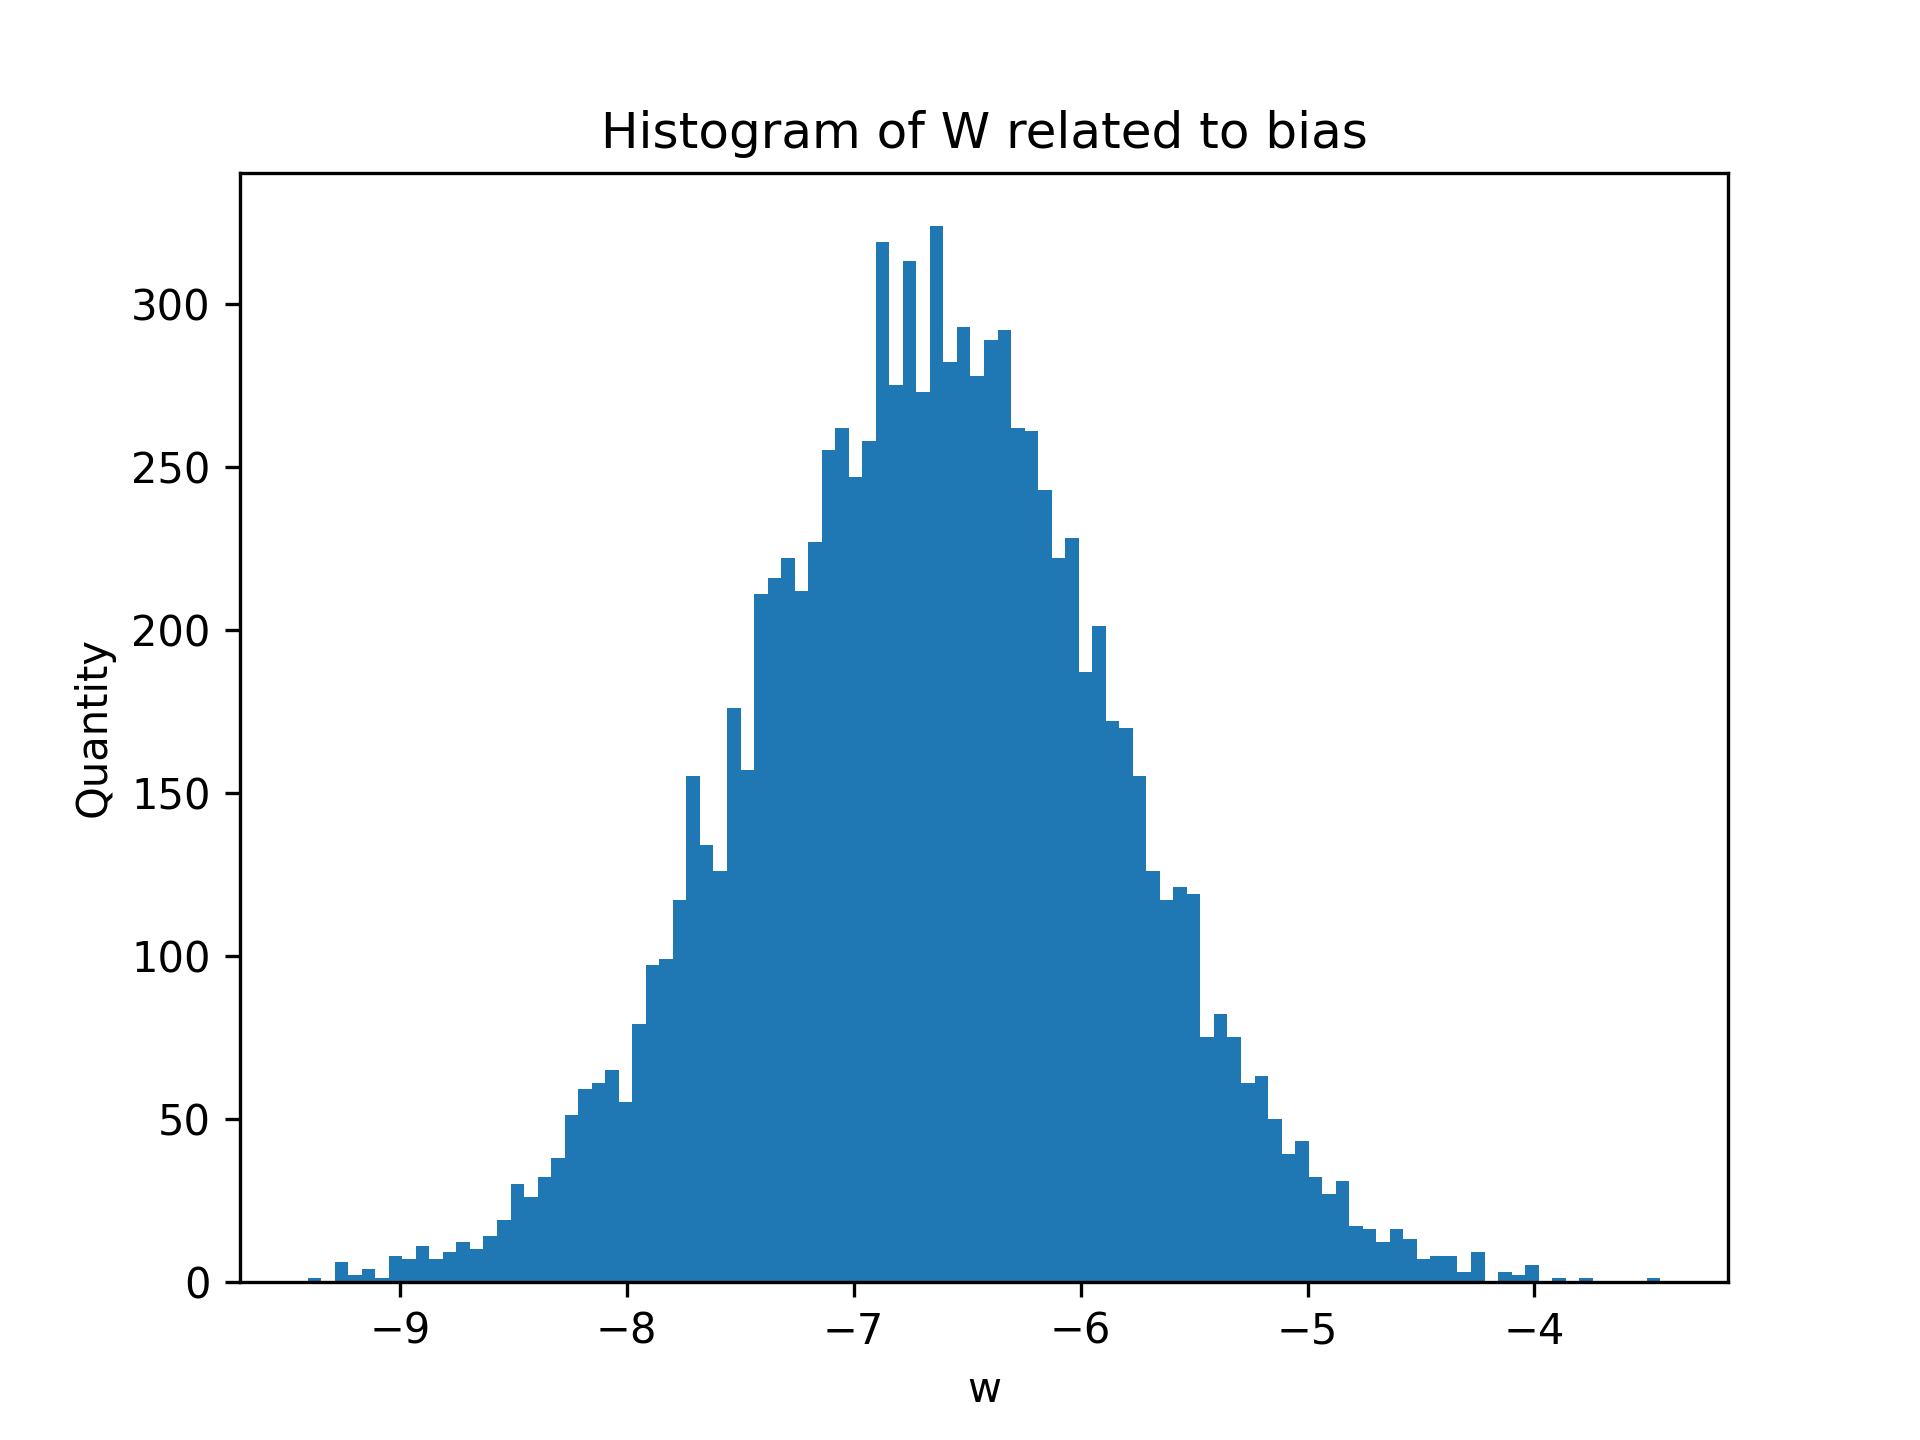
\includegraphics[width=\linewidth]{hist_featbias_349000000_sample_10000.png}
    \caption{$\alpha = 34.9$; $S = 10000$.}
  \end{subfigure}
  \hfill
  \begin{subfigure}[t]{0.24\textwidth}
    \centering
    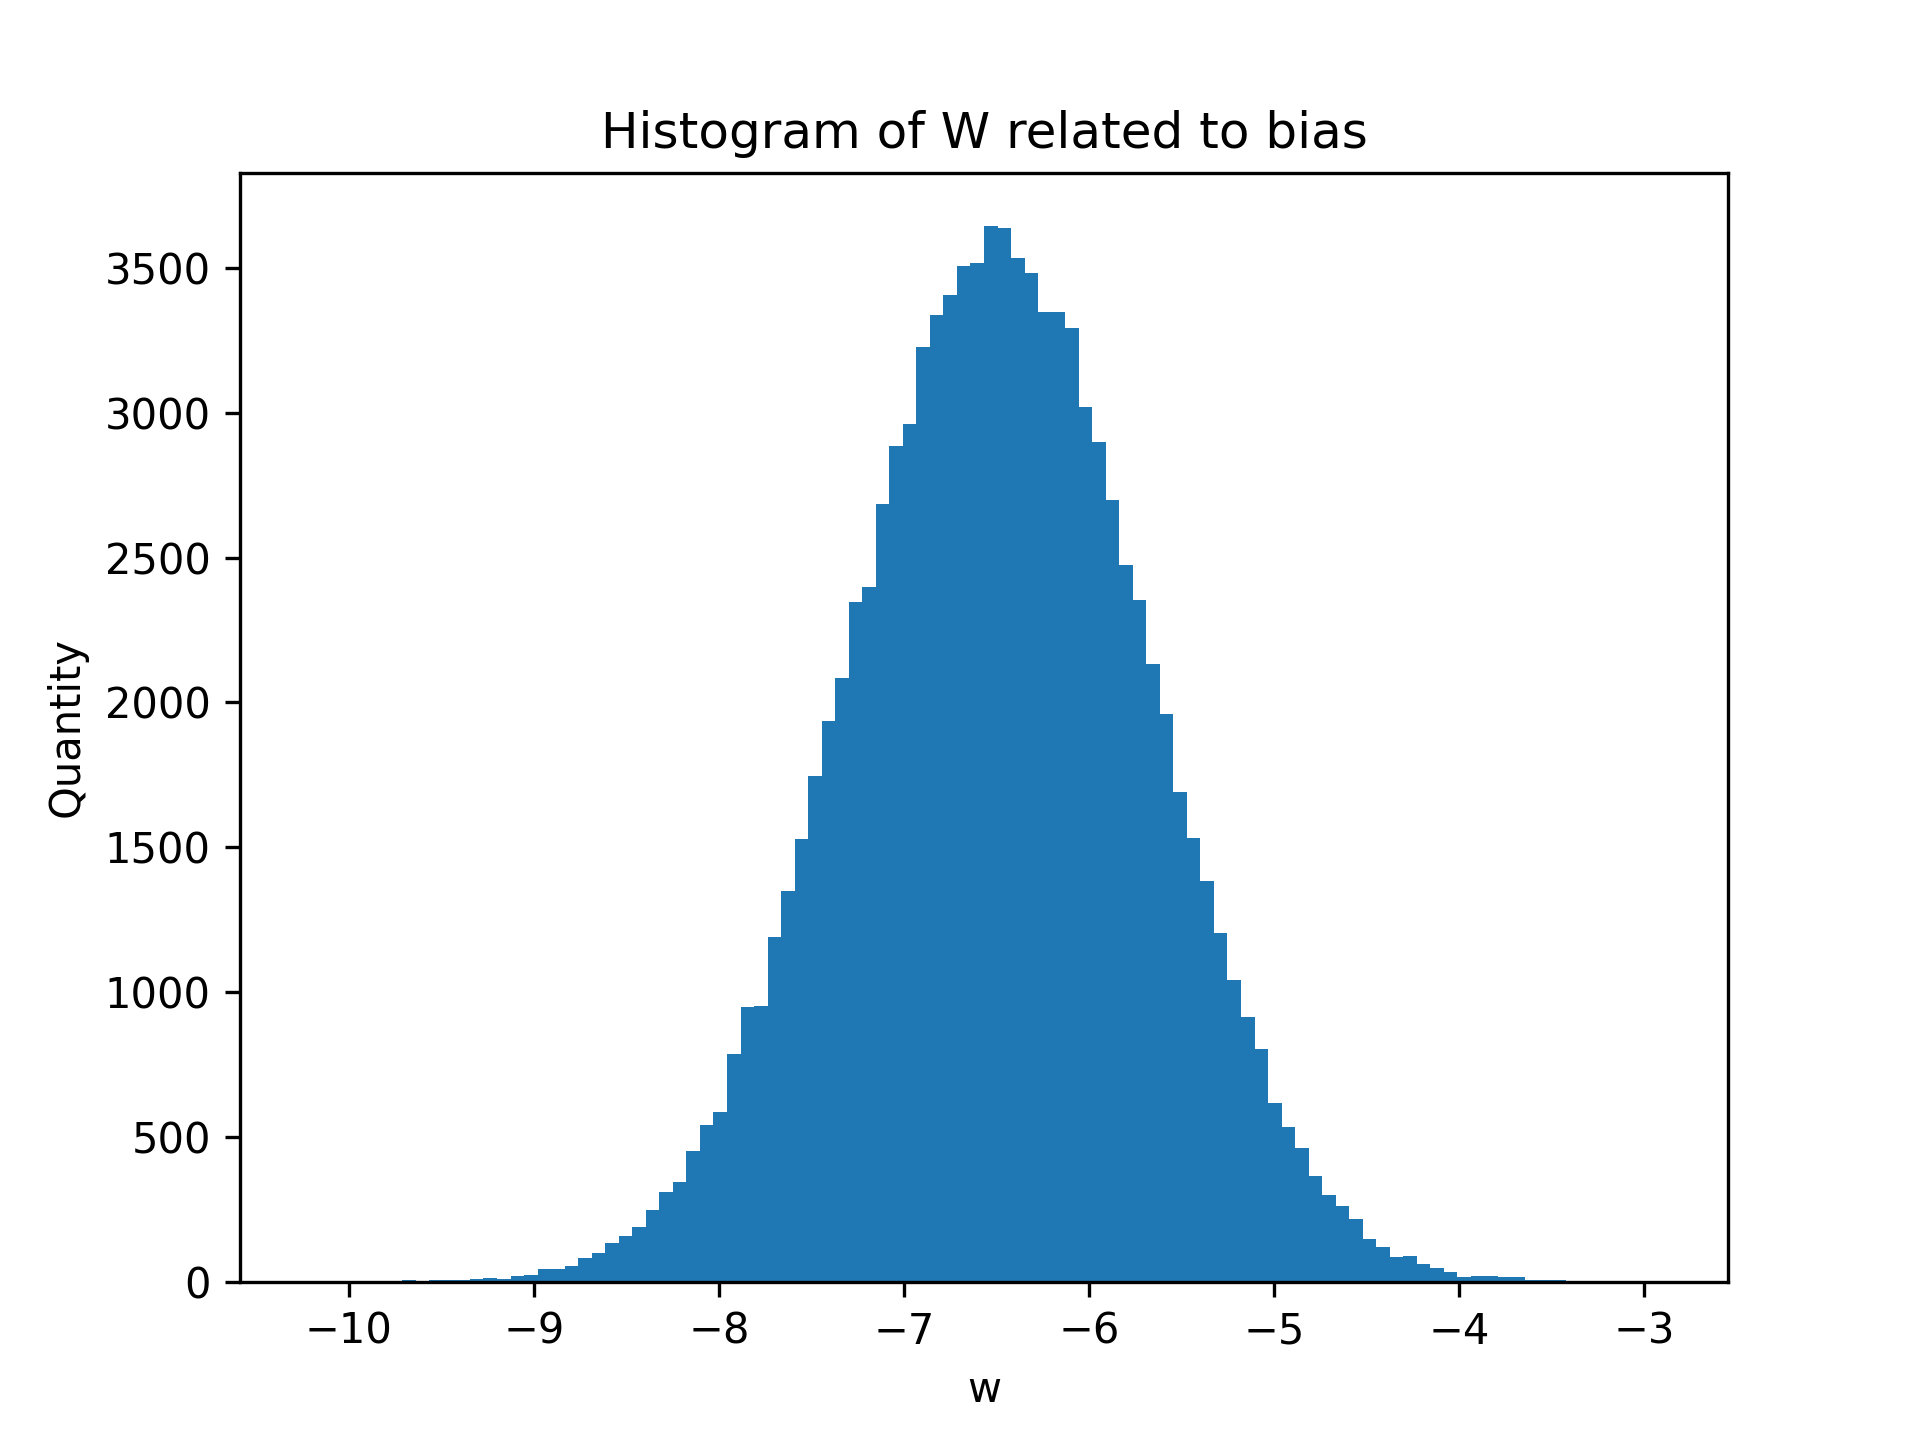
\includegraphics[width=\linewidth]{hist_featbias_349000000_sample_100000.png}
    \caption{$\alpha = 34.9$; $S = 100000$.}
  \end{subfigure}
  \caption{Histogram of W for bias with differents learning rates ($\alpha$) and sample sizes ($S$) for Monte Carlo approximation.}
  \label{fig:hist_featbias}
\end{figure}

% Histogram - Feature 1
\begin{figure}
  \centering
  \begin{subfigure}[t]{0.24\textwidth}
    \centering
    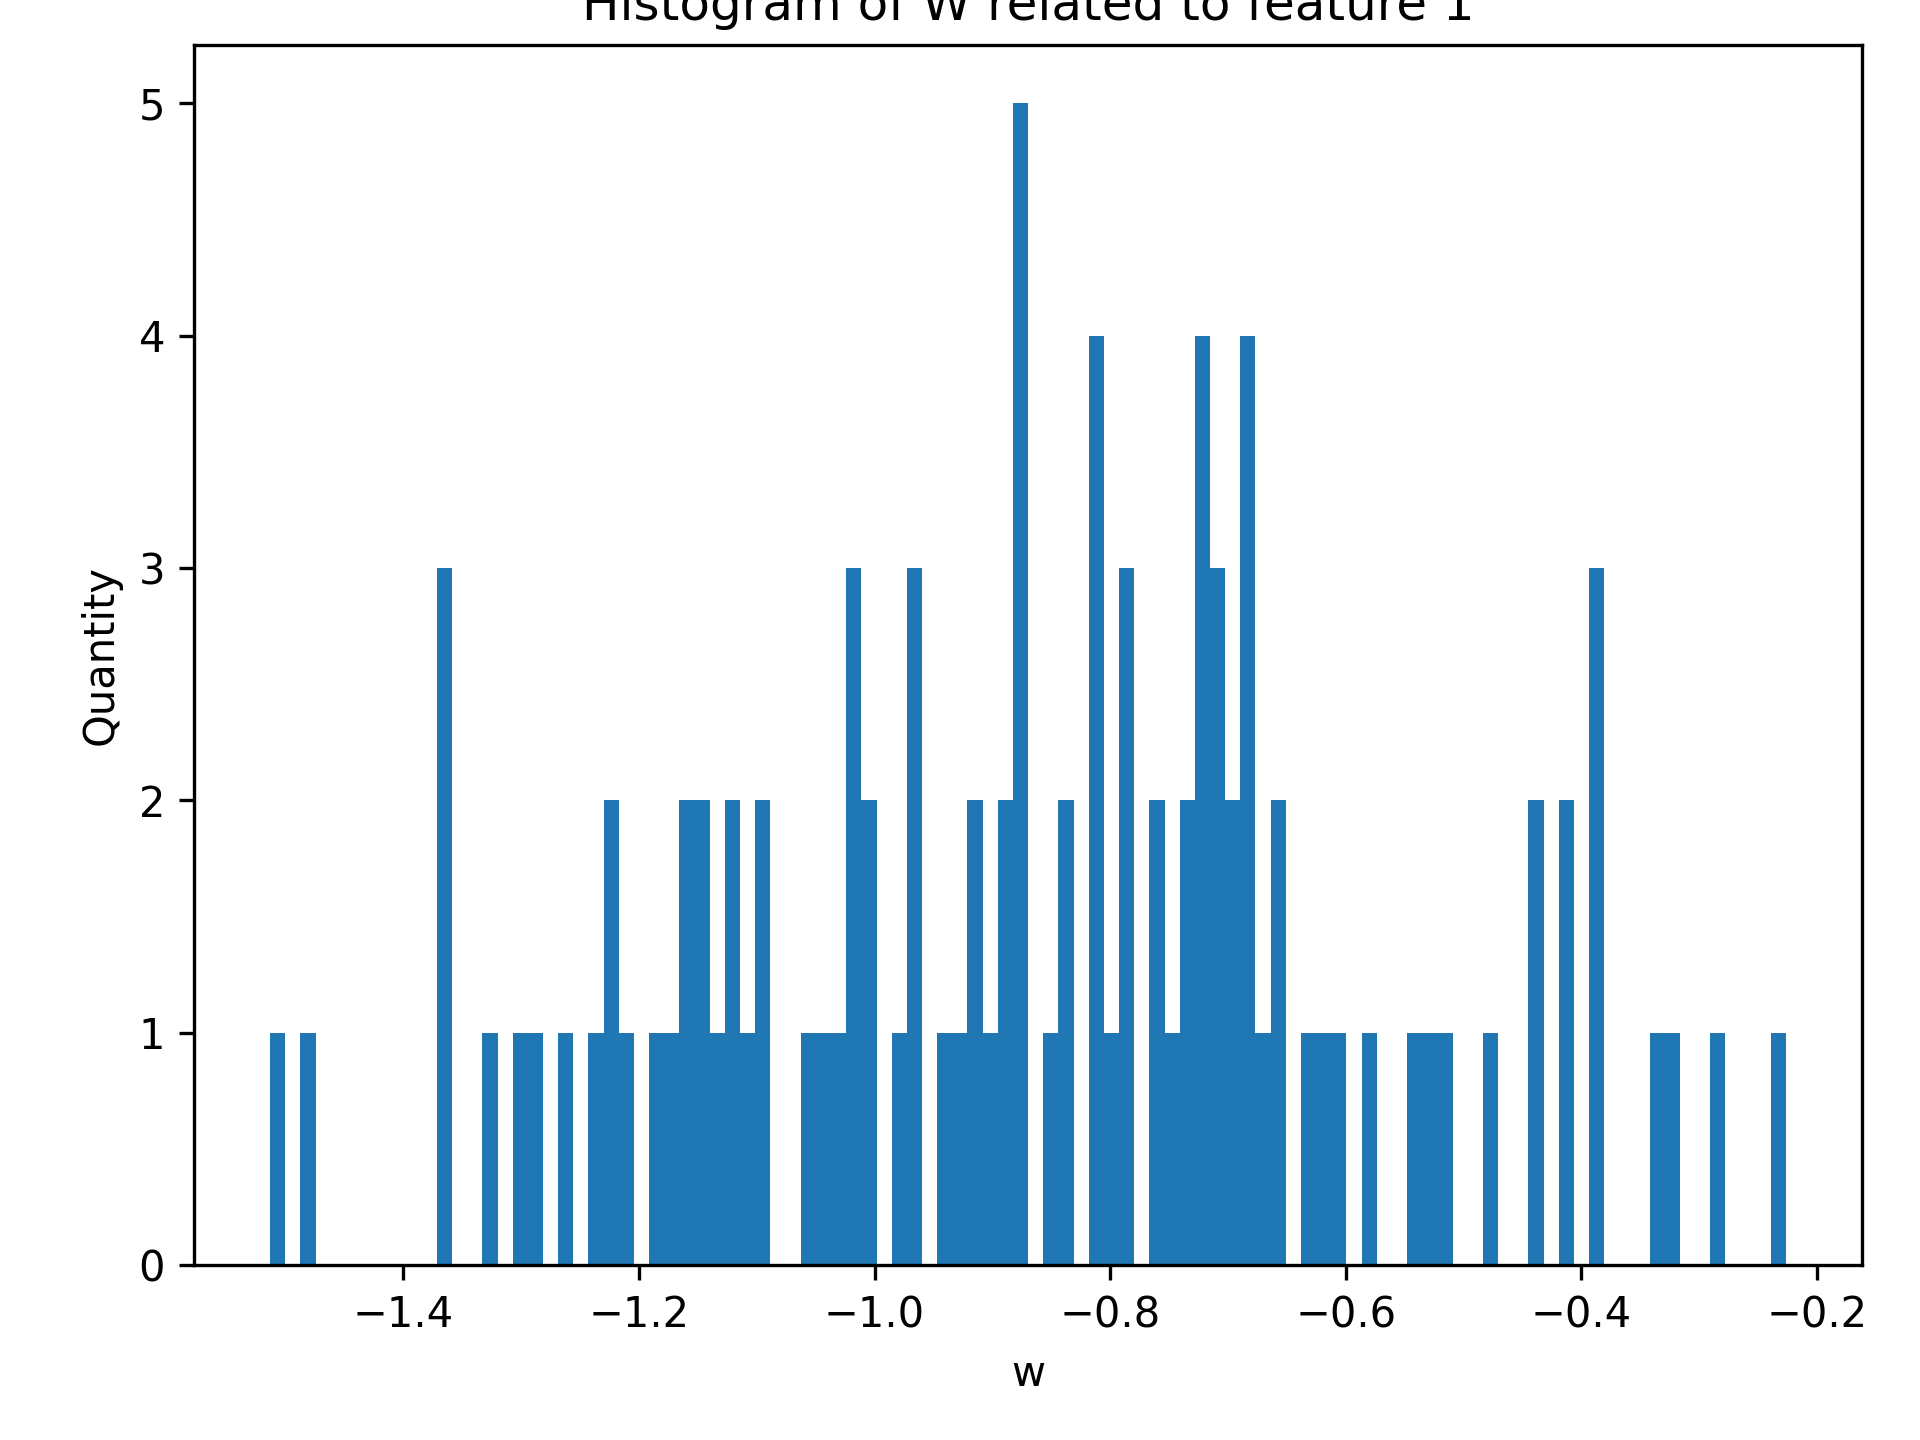
\includegraphics[width=\linewidth]{hist_feat0_1_sample_100.png}
    \caption{$\alpha = 1e-7$; $S = 100$.}
  \end{subfigure}
  \hfill
  \begin{subfigure}[t]{0.24\textwidth}
    \centering
    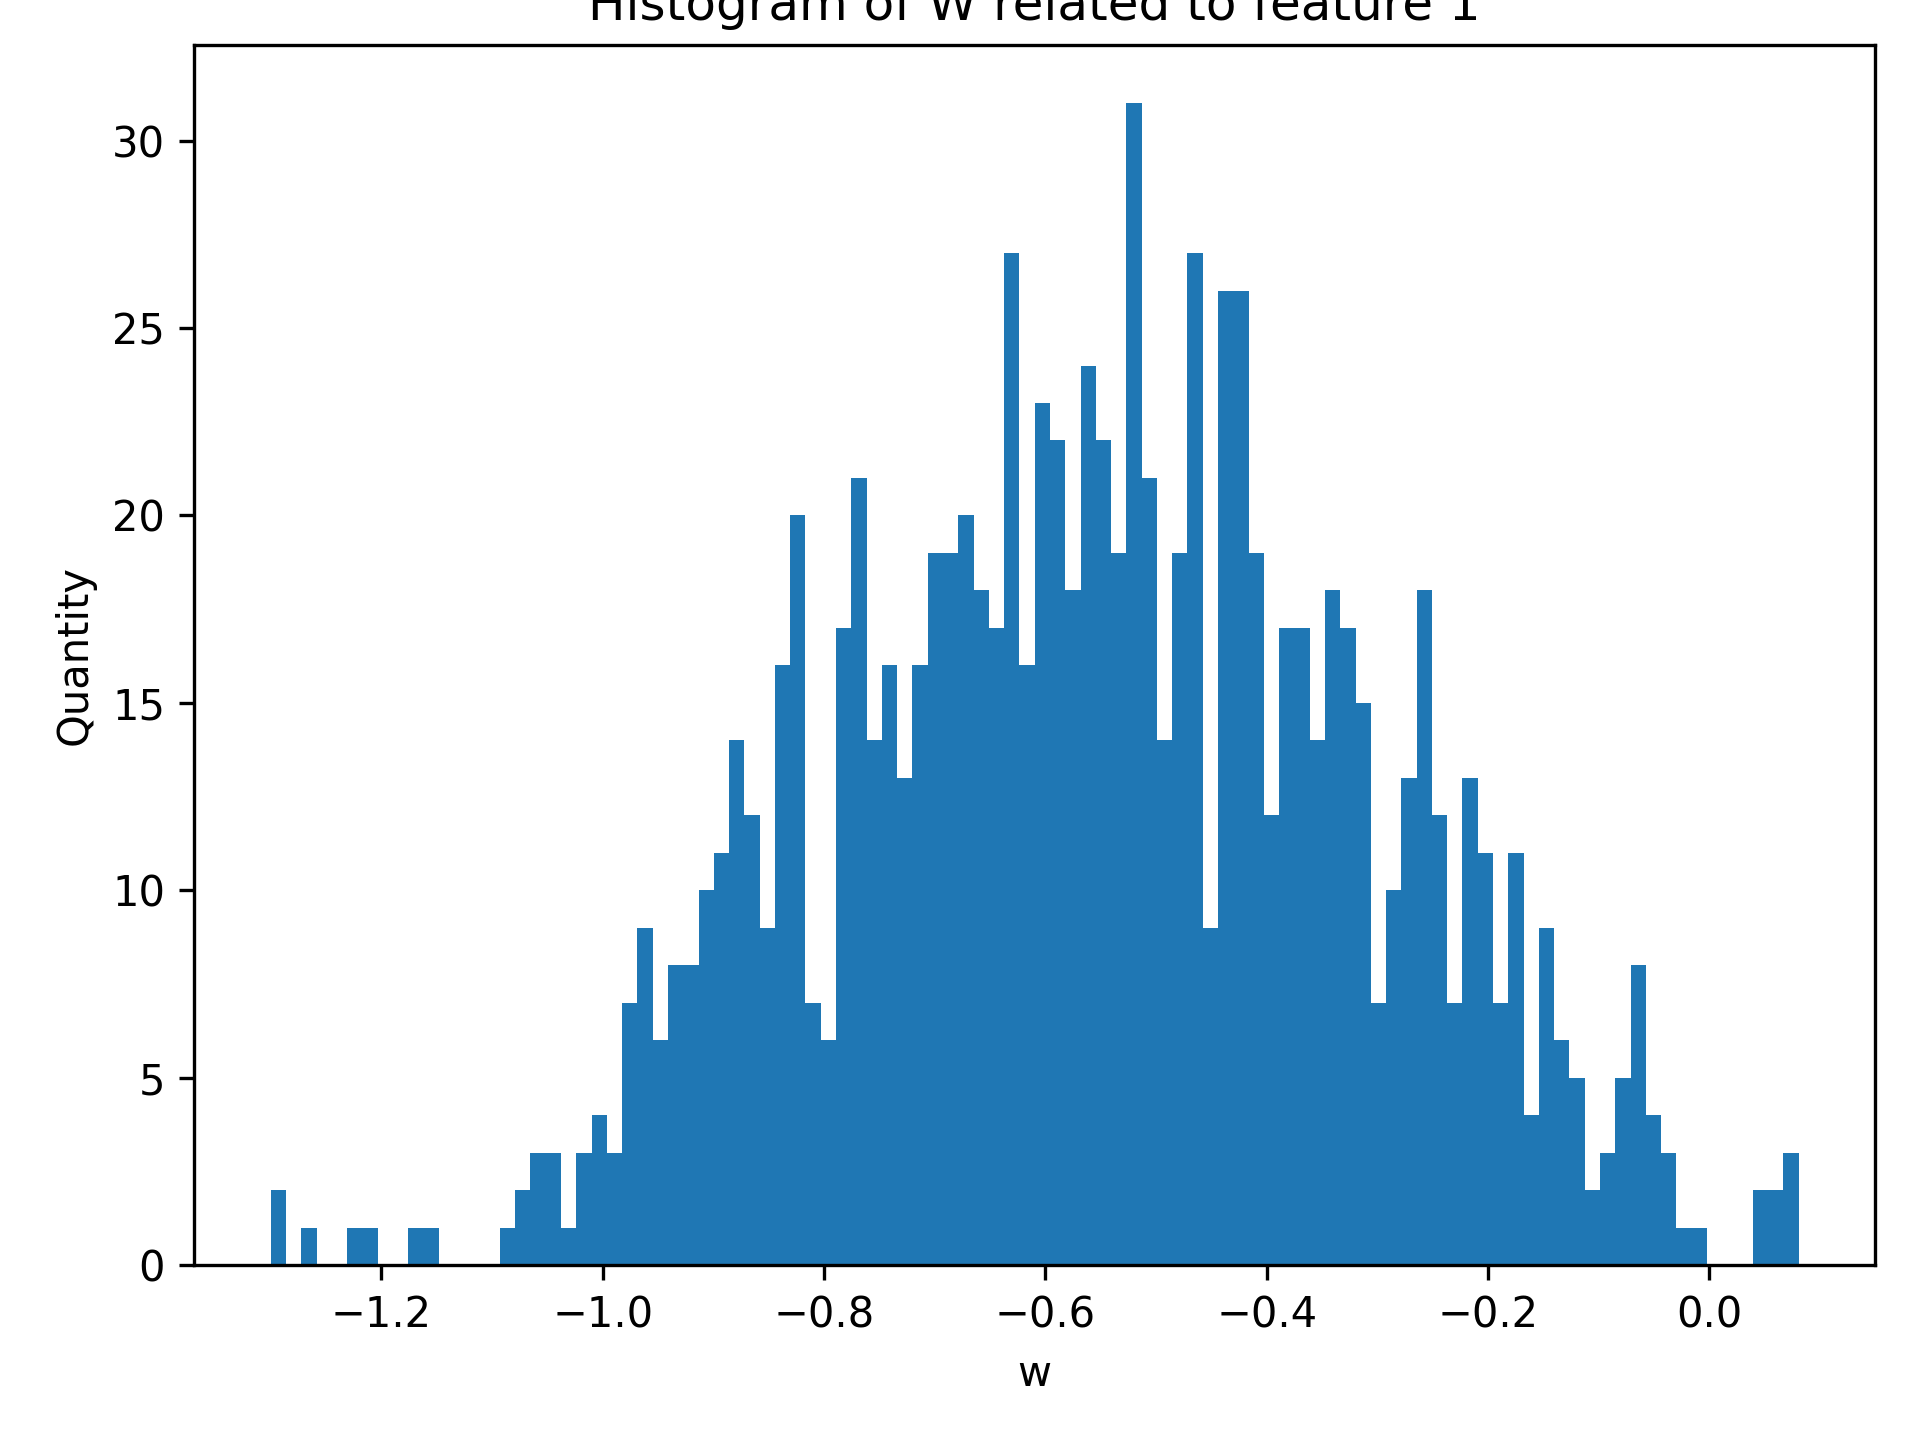
\includegraphics[width=\linewidth]{hist_feat0_1_sample_1000.png}
    \caption{$\alpha = 1e-7$; $S = 1000$.}
  \end{subfigure}
  \hfill
  \begin{subfigure}[t]{0.24\textwidth}
    \centering
    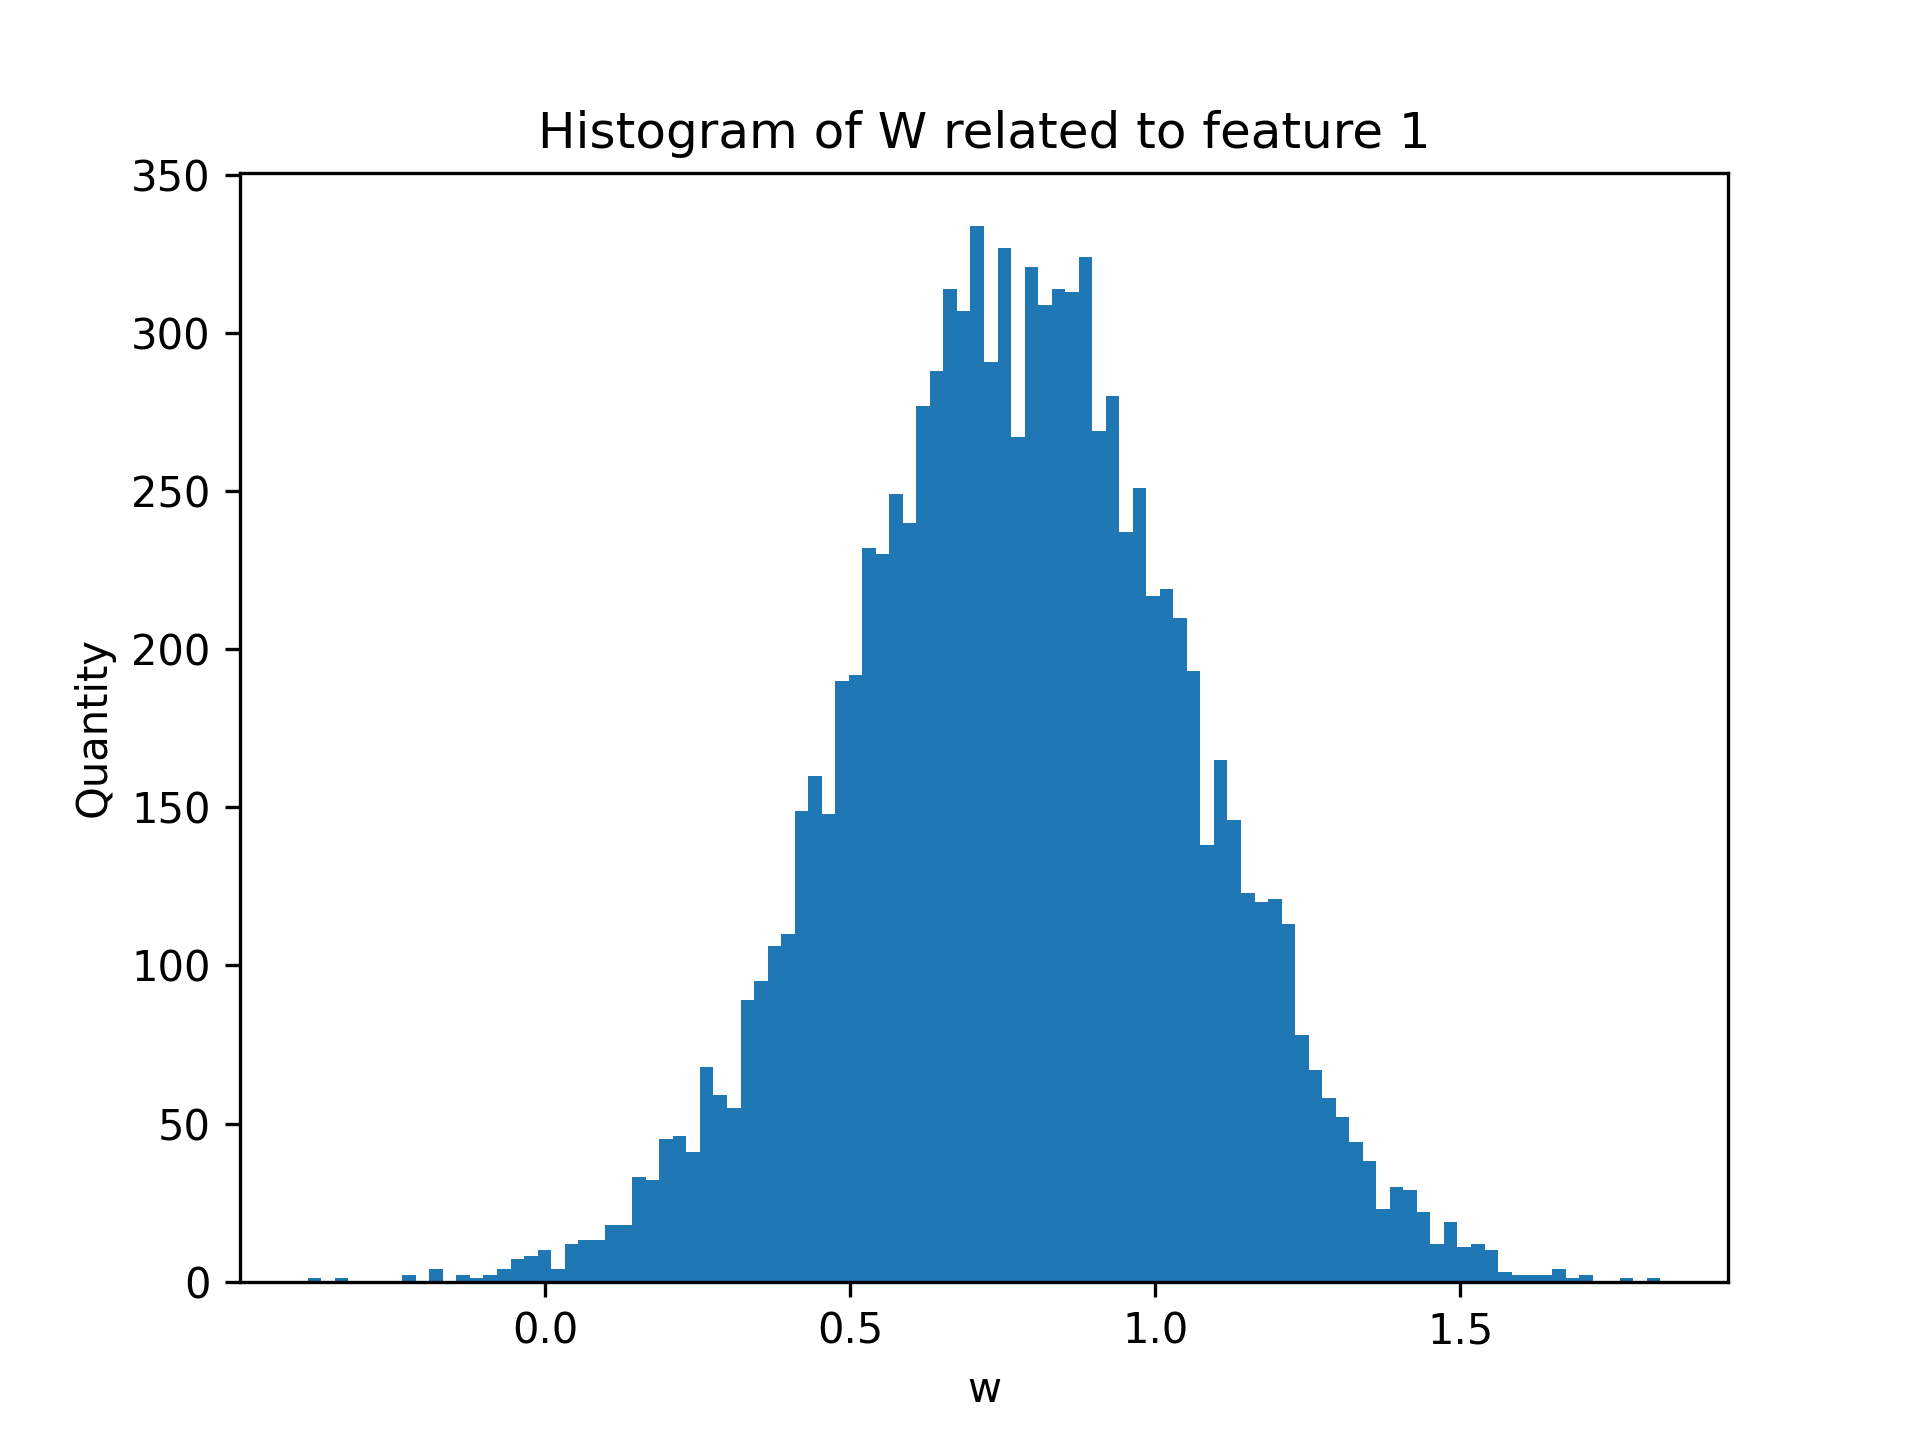
\includegraphics[width=\linewidth]{hist_feat0_1_sample_10000.png}
    \caption{$\alpha = 1e-7$; $S = 10000$.}
  \end{subfigure}
  \hfill
  \begin{subfigure}[t]{0.24\textwidth}
    \centering
    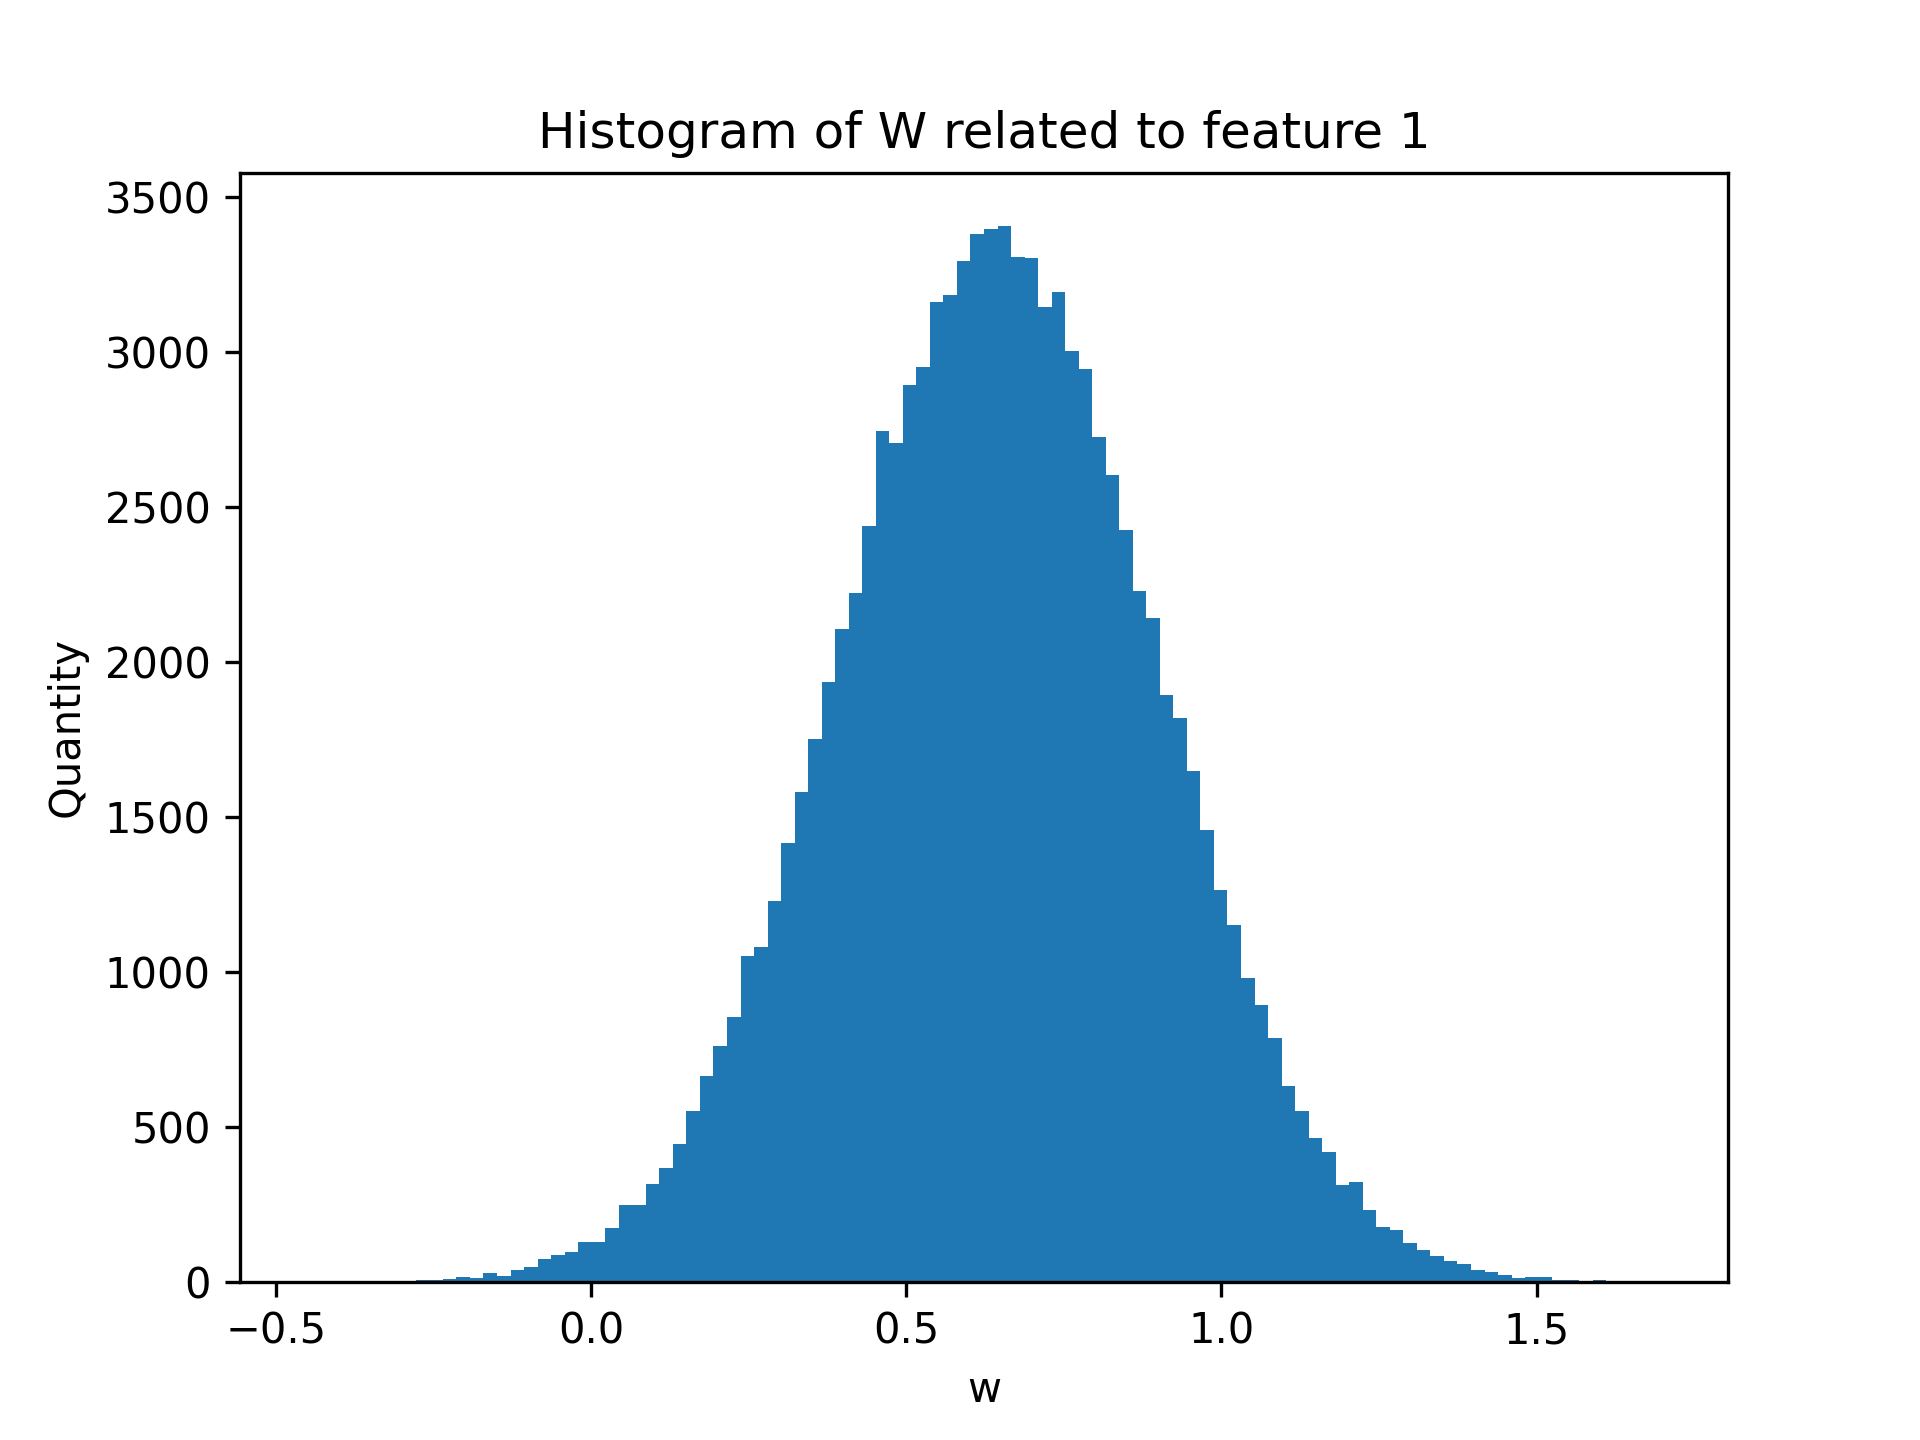
\includegraphics[width=\linewidth]{hist_feat0_1_sample_100000.png}
    \caption{$\alpha = 1e-7$; $S = 100000$.}
  \end{subfigure}
  % \hfill
  \begin{subfigure}[t]{0.24\textwidth}
    \centering
    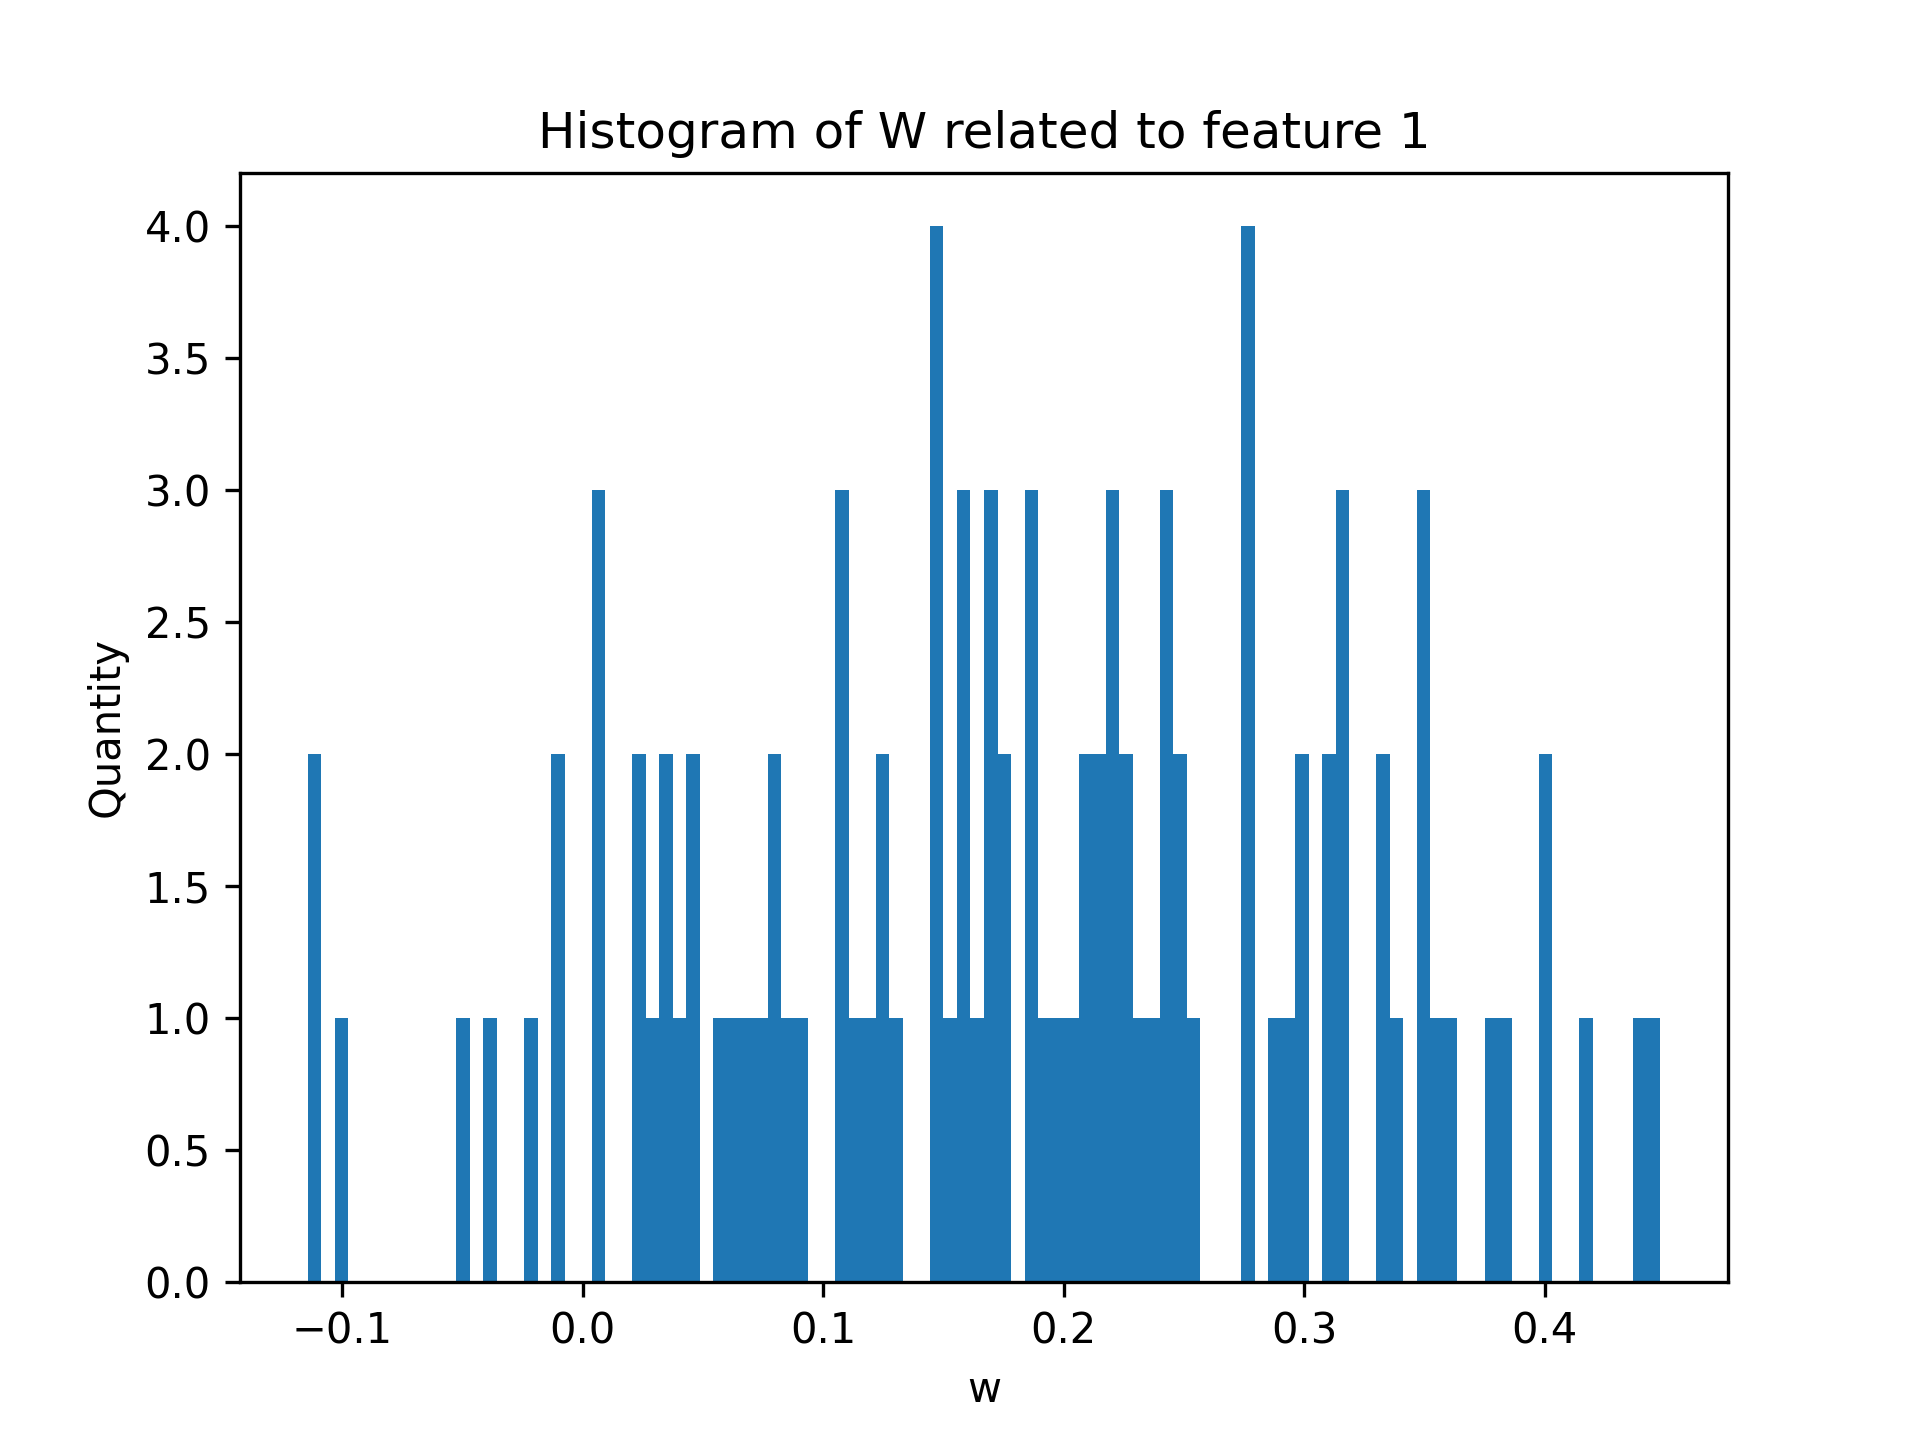
\includegraphics[width=\linewidth]{hist_feat0_10000_sample_100.png}
    \caption{$\alpha = 1e-3$; $S = 100$.}
  \end{subfigure}
  \hfill
  \begin{subfigure}[t]{0.24\textwidth}
    \centering
    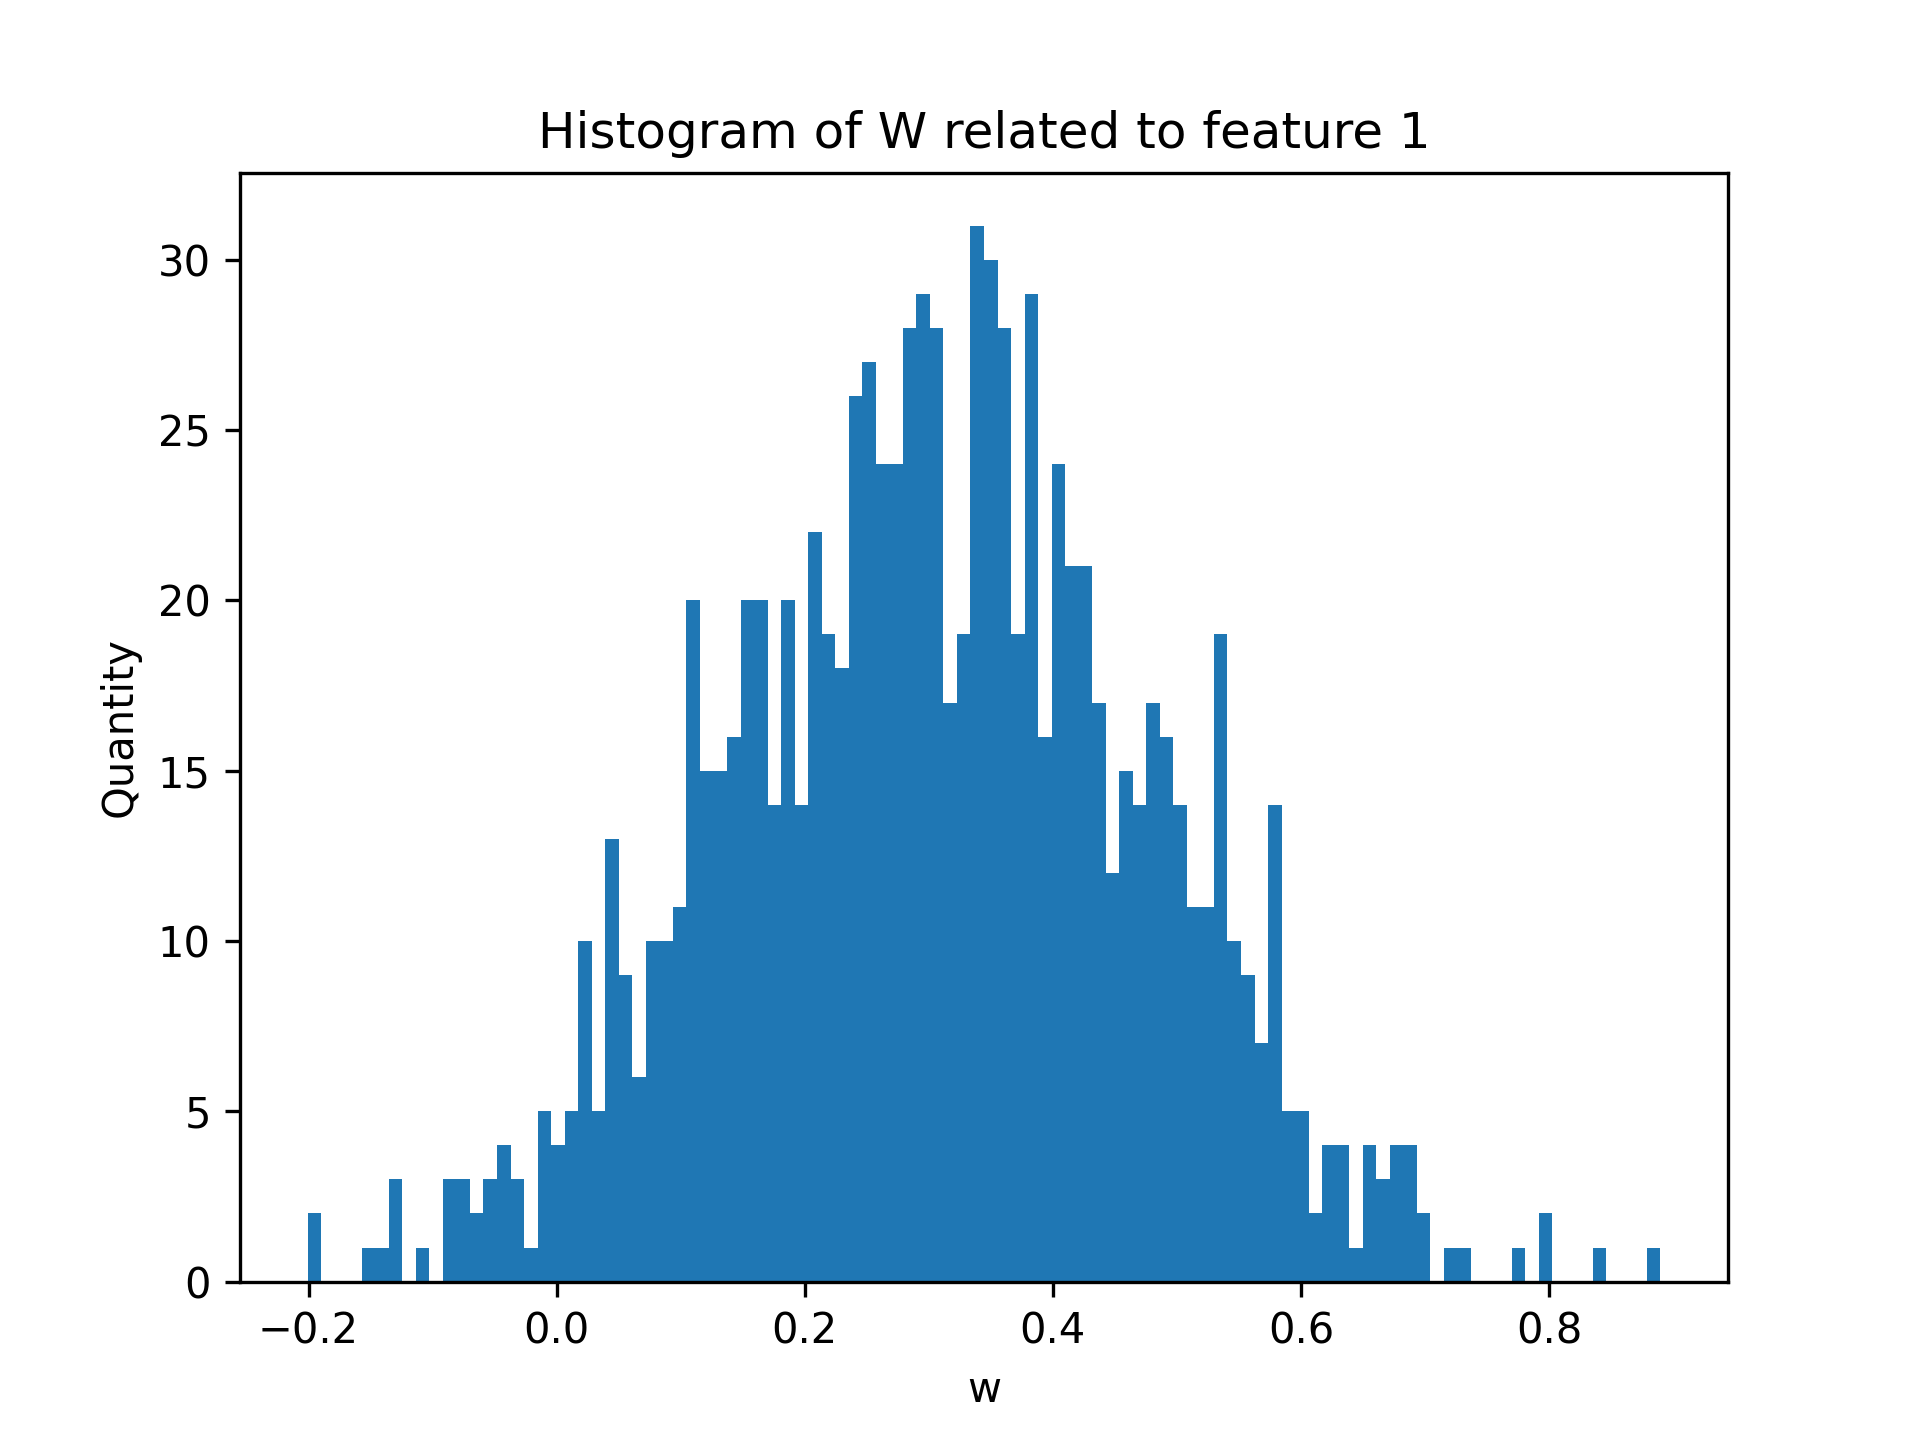
\includegraphics[width=\linewidth]{hist_feat0_10000_sample_1000.png}
    \caption{$\alpha = 1e-3$; $S = 1000$.}
  \end{subfigure}
  \hfill
  \begin{subfigure}[t]{0.24\textwidth}
    \centering
    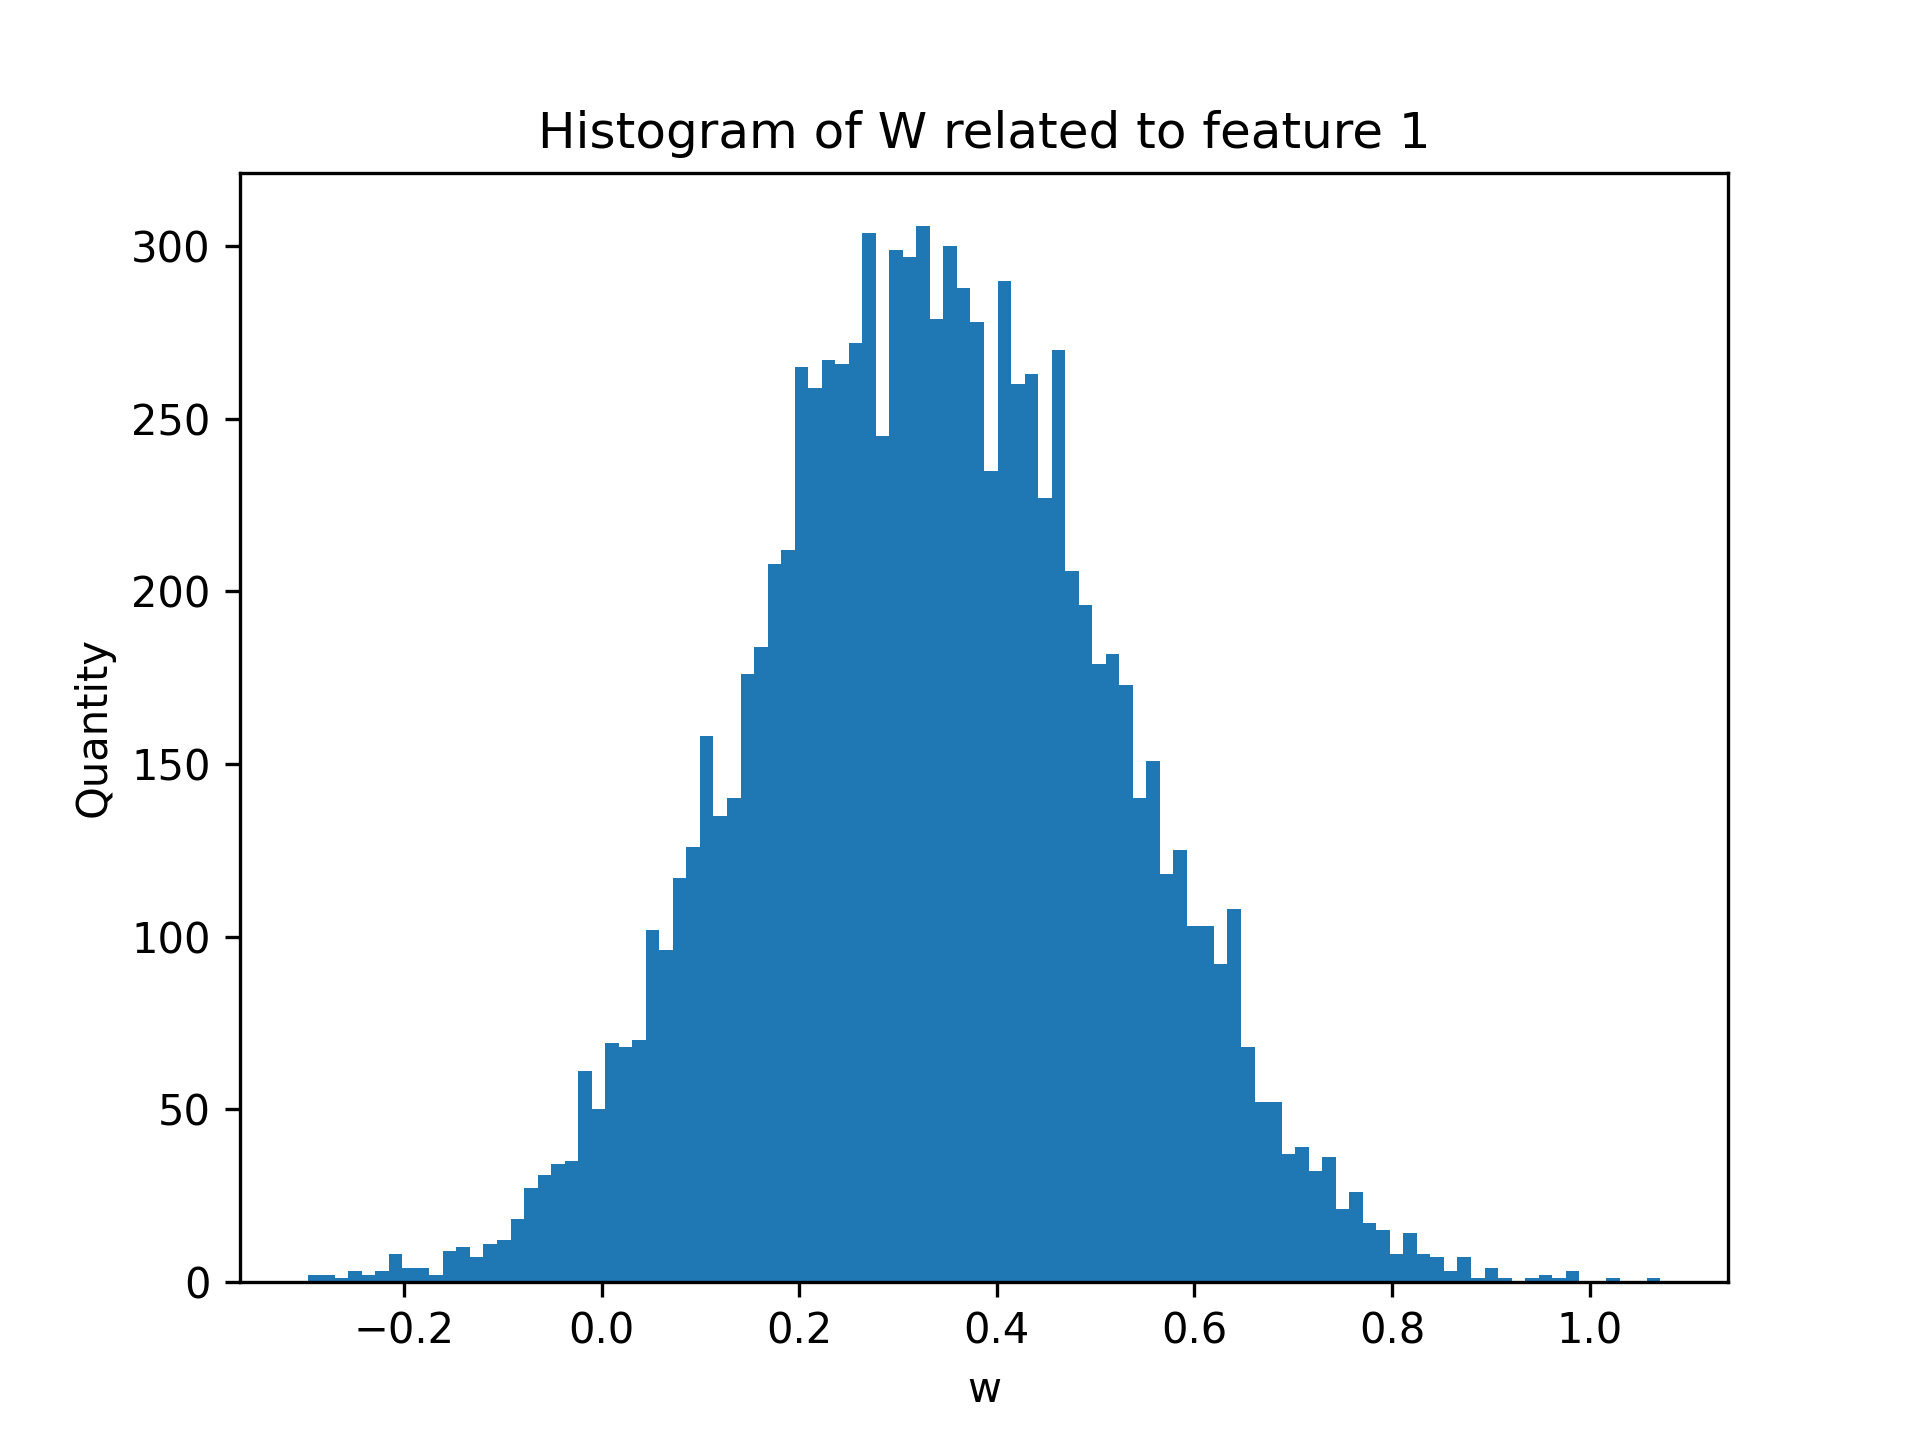
\includegraphics[width=\linewidth]{hist_feat0_10000_sample_10000.png}
    \caption{$\alpha = 1e-3$; $S = 10000$.}
  \end{subfigure}
  \hfill
  \begin{subfigure}[t]{0.24\textwidth}
    \centering
    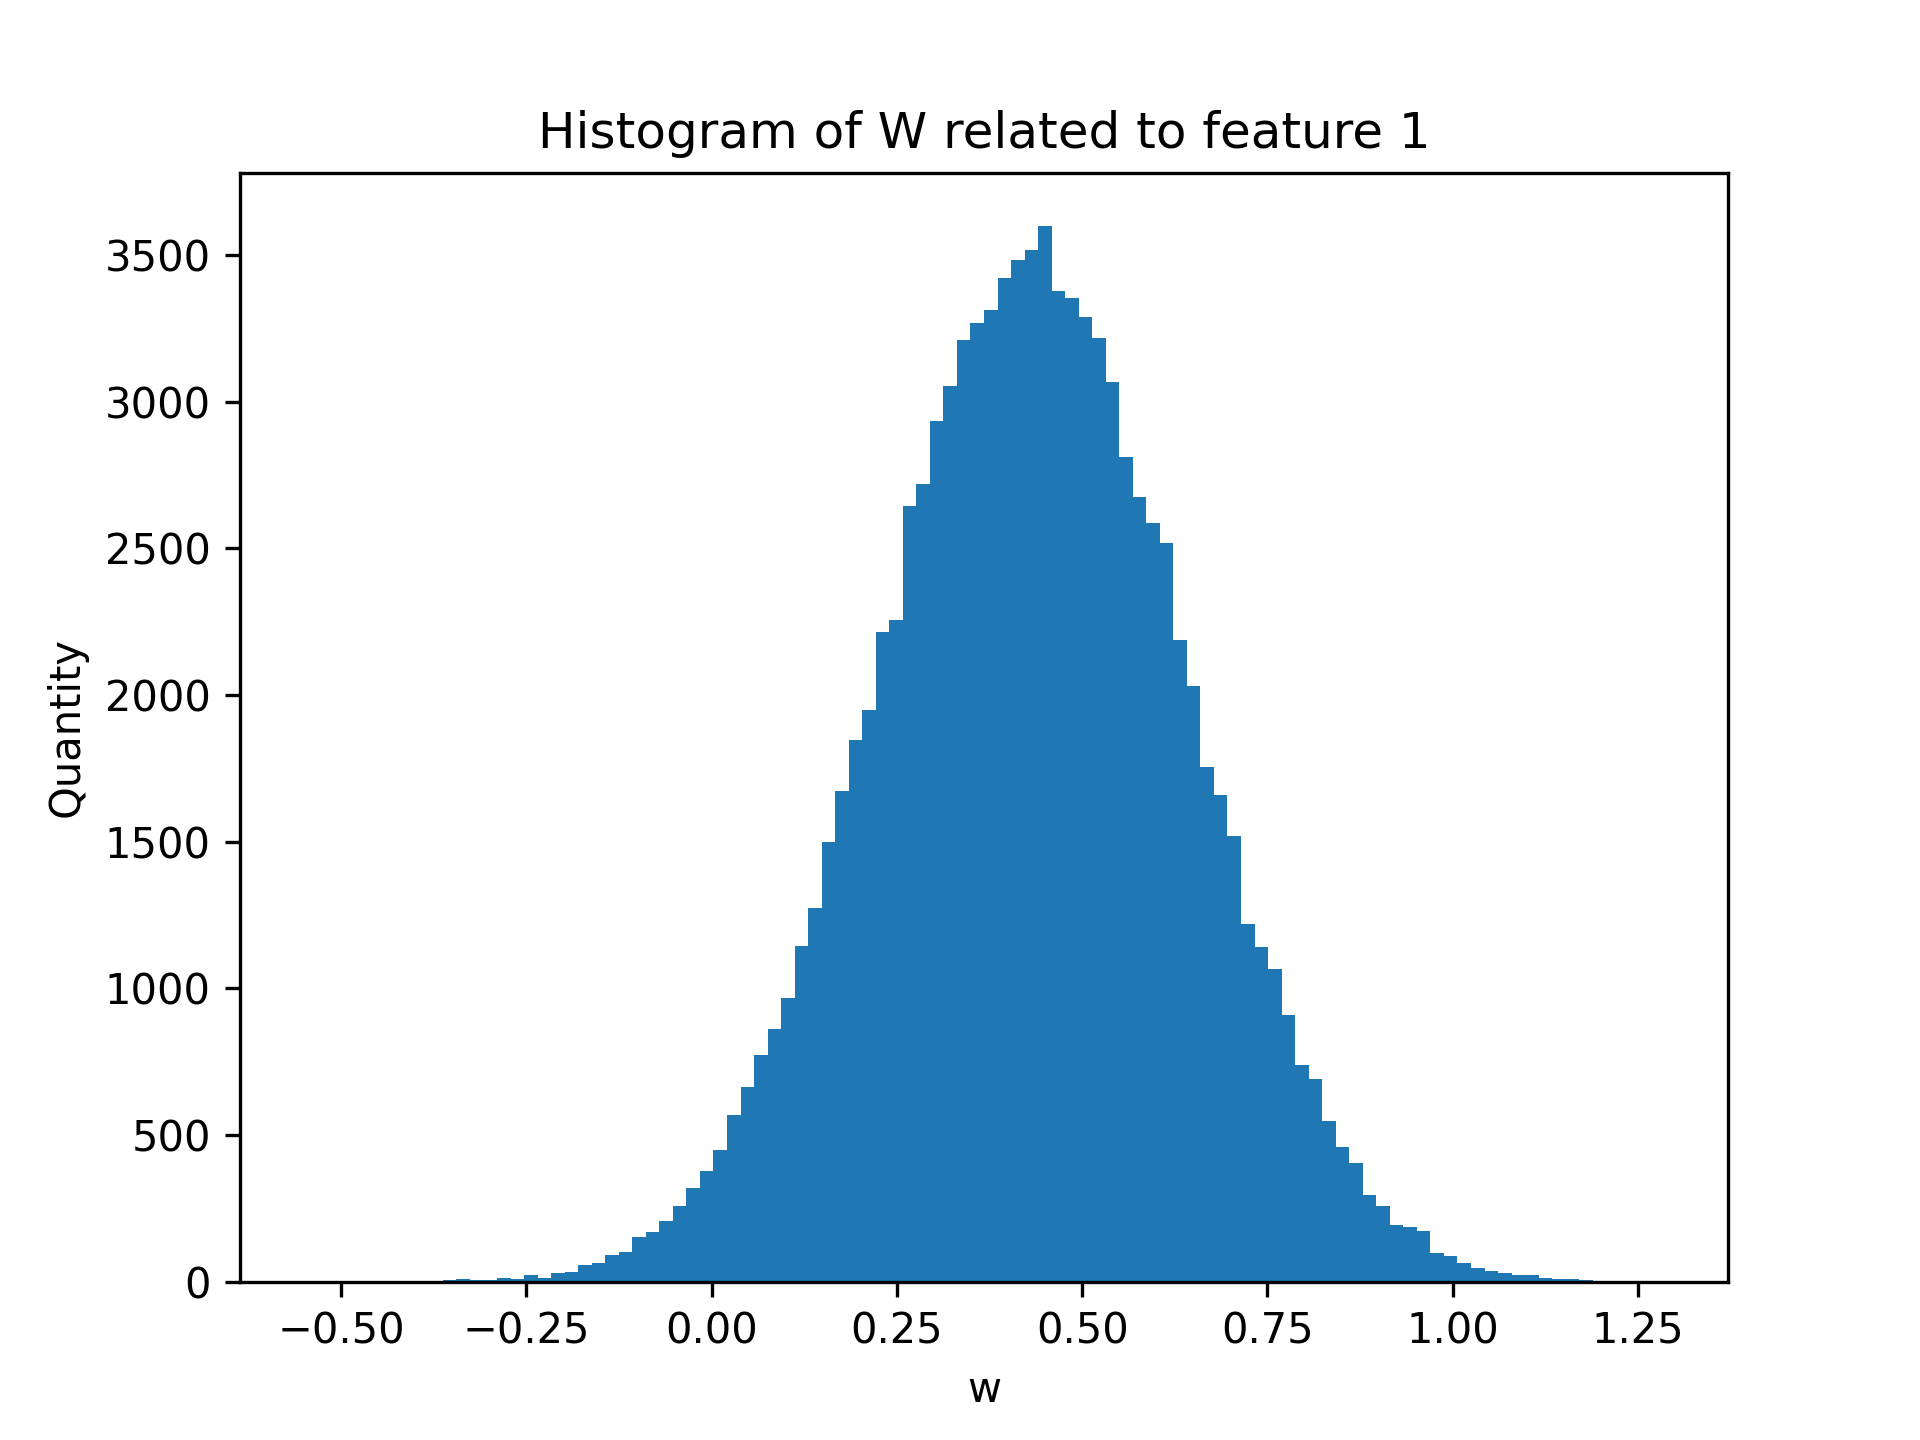
\includegraphics[width=\linewidth]{hist_feat0_10000_sample_100000.png}
    \caption{$\alpha = 1e-3$; $S = 100000$.}
  \end{subfigure}
  % \hfill
  \begin{subfigure}[t]{0.24\textwidth}
    \centering
    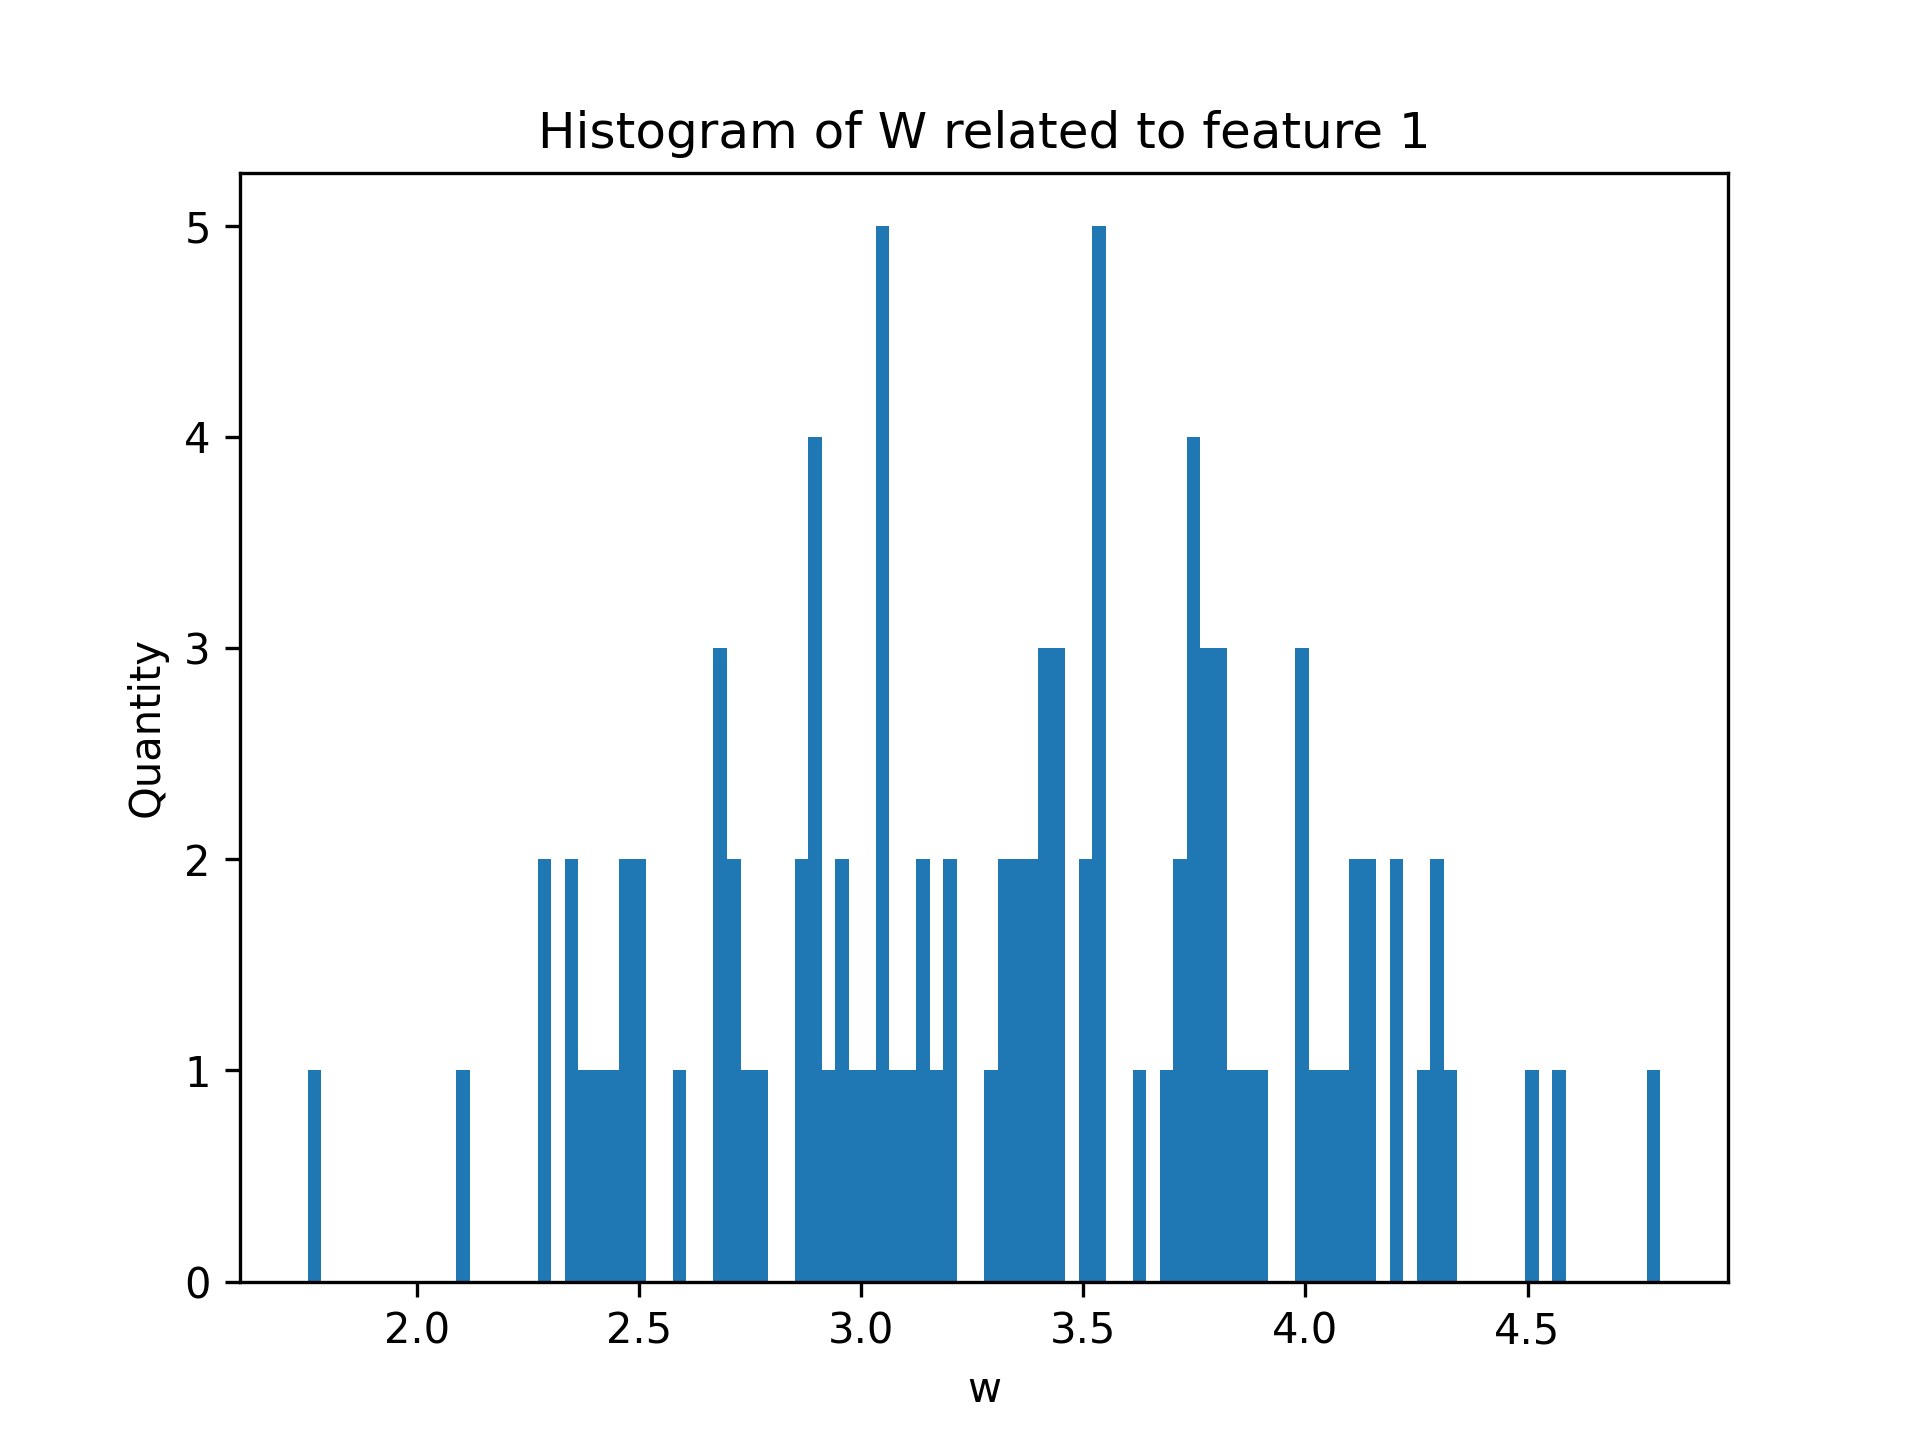
\includegraphics[width=\linewidth]{hist_feat0_349000000_sample_100.png}
    \caption{$\alpha = 34.9$; $S = 100$.}
  \end{subfigure}
  \hfill
  \begin{subfigure}[t]{0.24\textwidth}
    \centering
    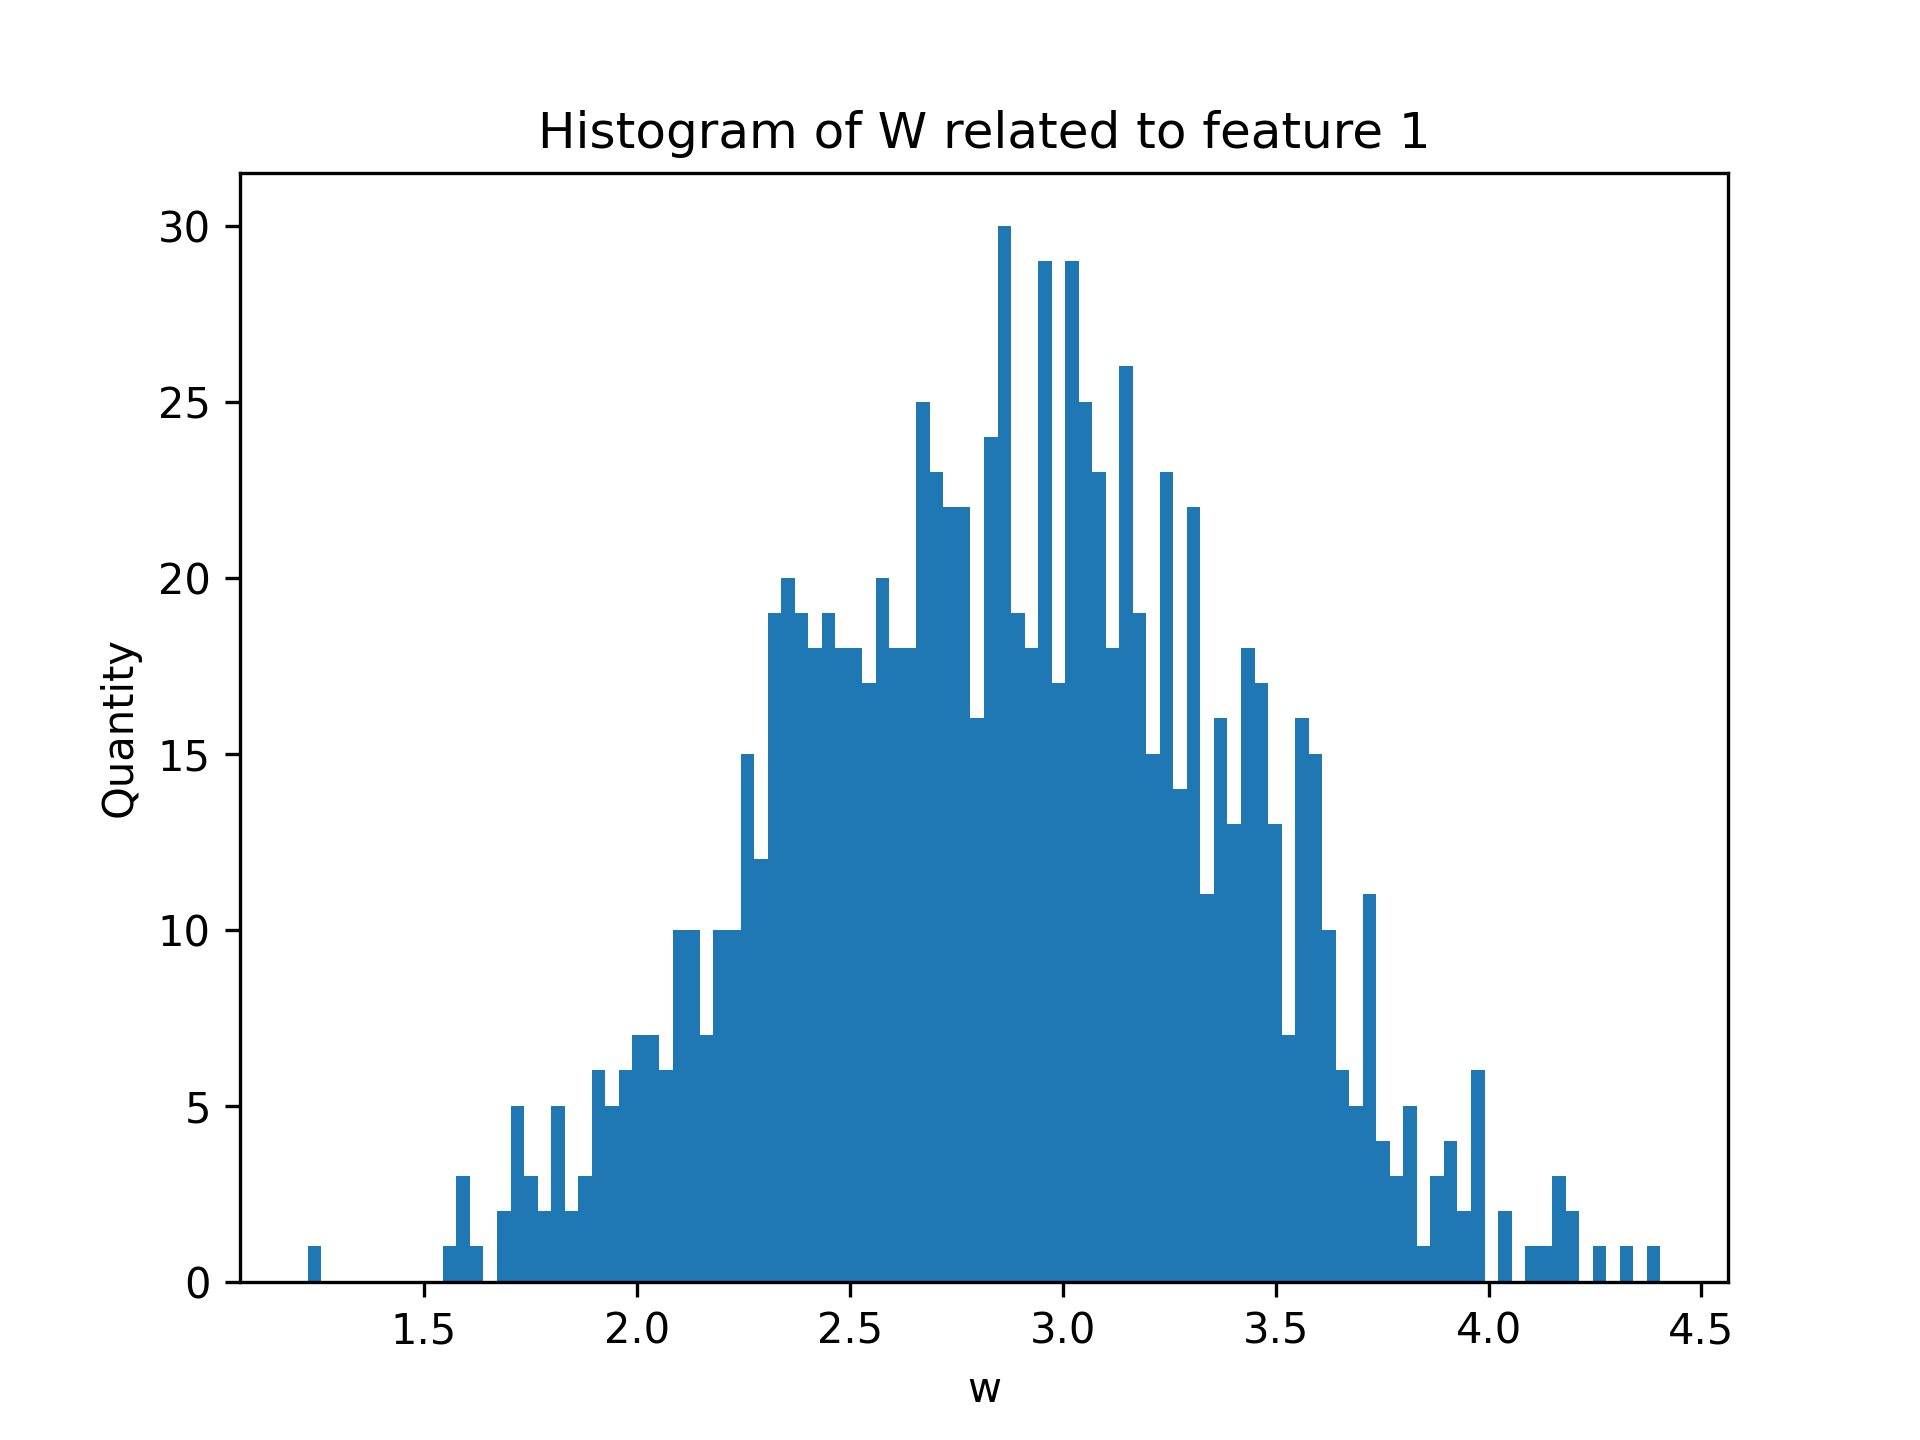
\includegraphics[width=\linewidth]{hist_feat0_349000000_sample_1000.png}
    \caption{$\alpha = 34.9$; $S = 1000$.}
  \end{subfigure}
  \hfill
  \begin{subfigure}[t]{0.24\textwidth}
    \centering
    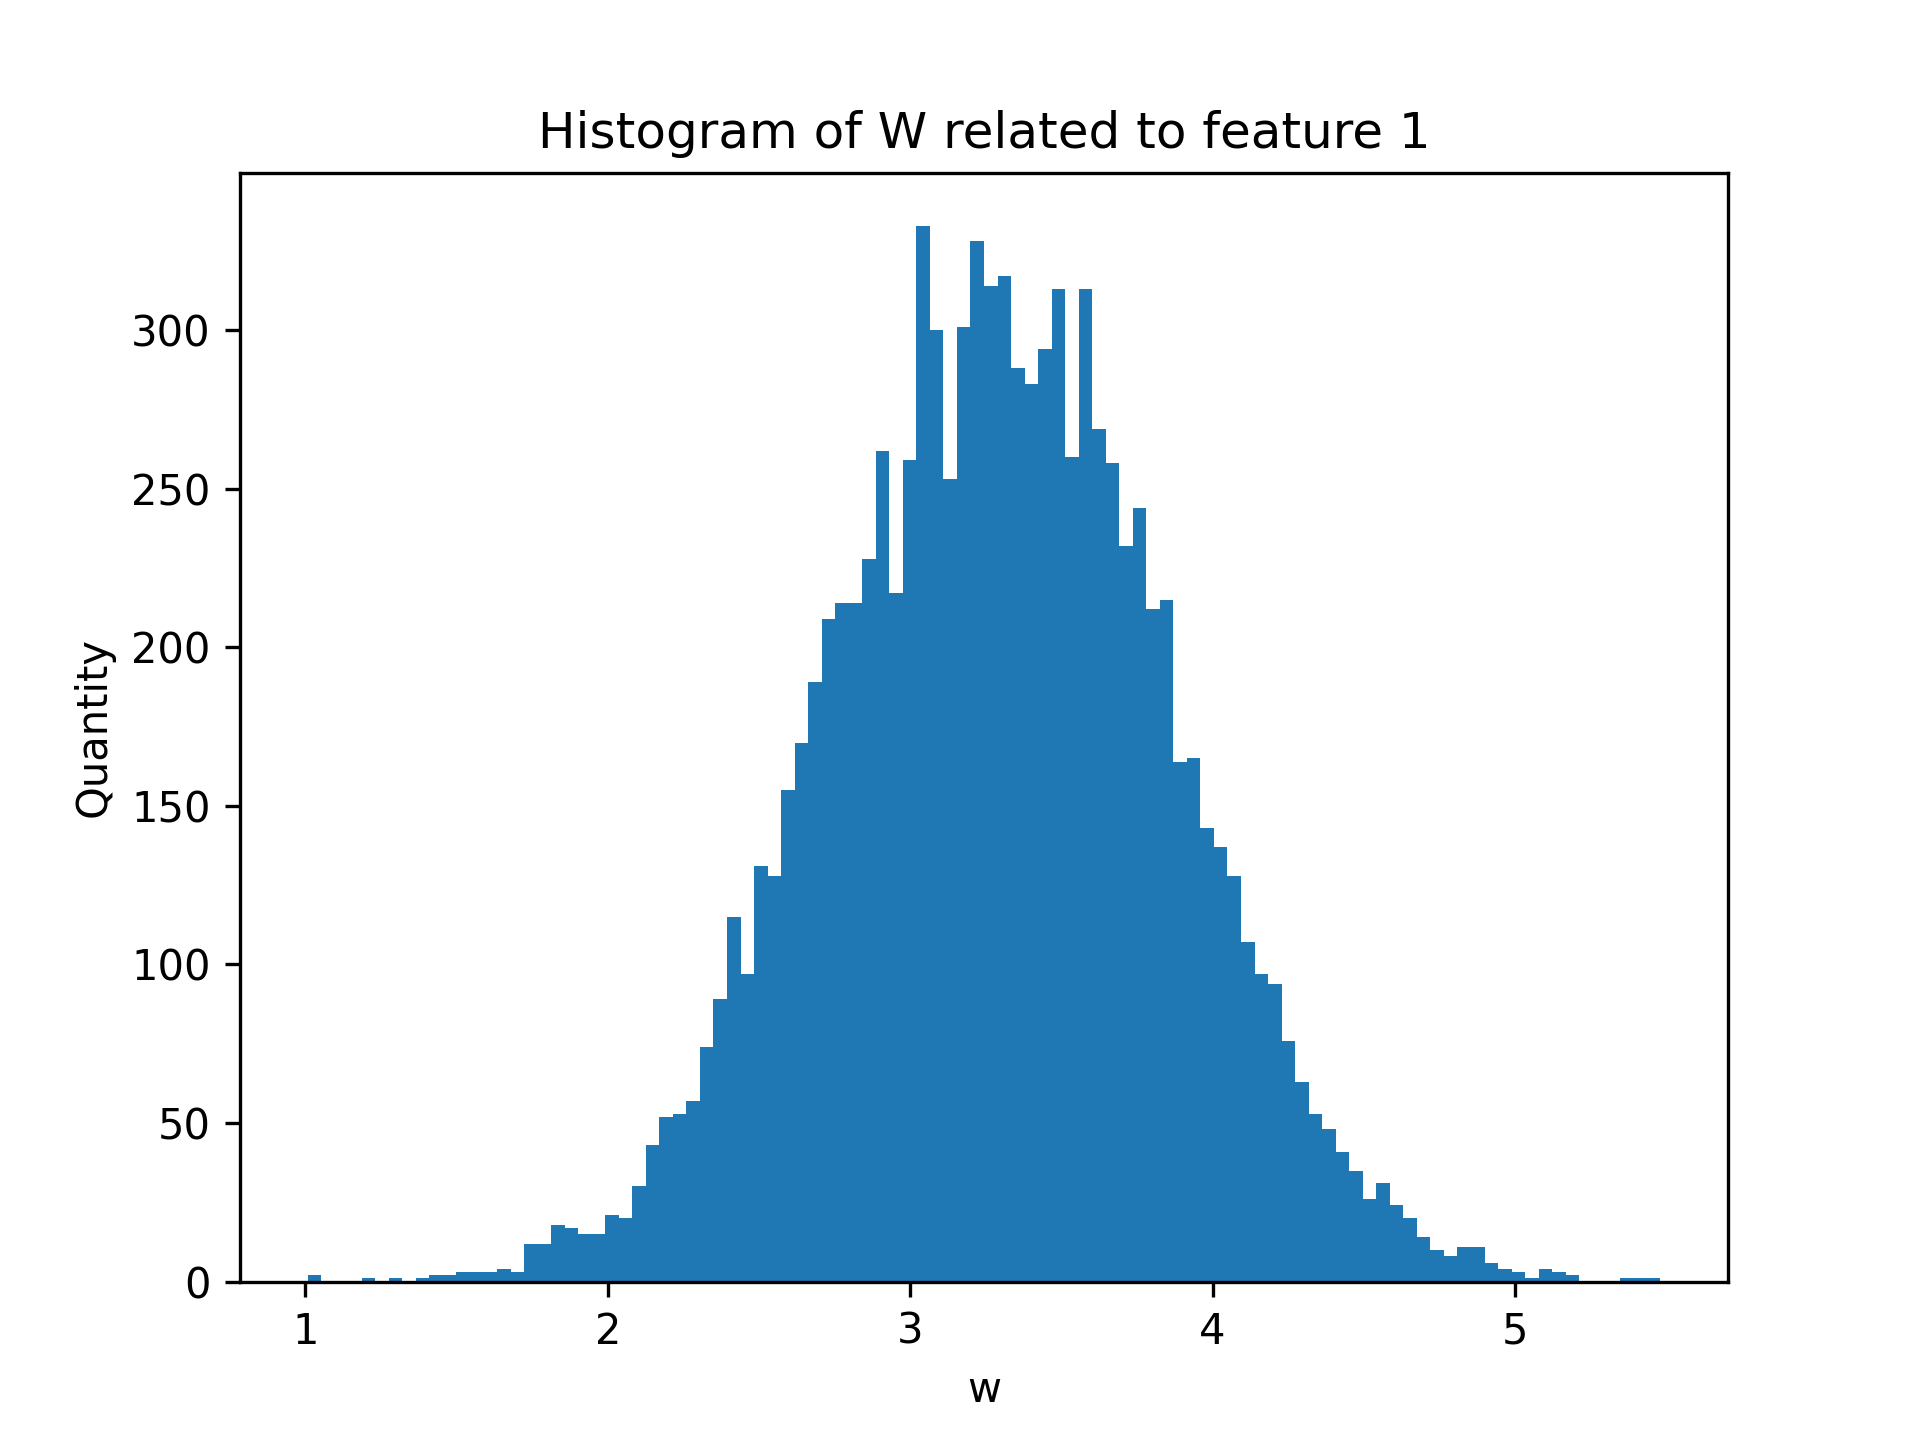
\includegraphics[width=\linewidth]{hist_feat0_349000000_sample_10000.png}
    \caption{$\alpha = 34.9$; $S = 10000$.}
  \end{subfigure}
  \hfill
  \begin{subfigure}[t]{0.24\textwidth}
    \centering
    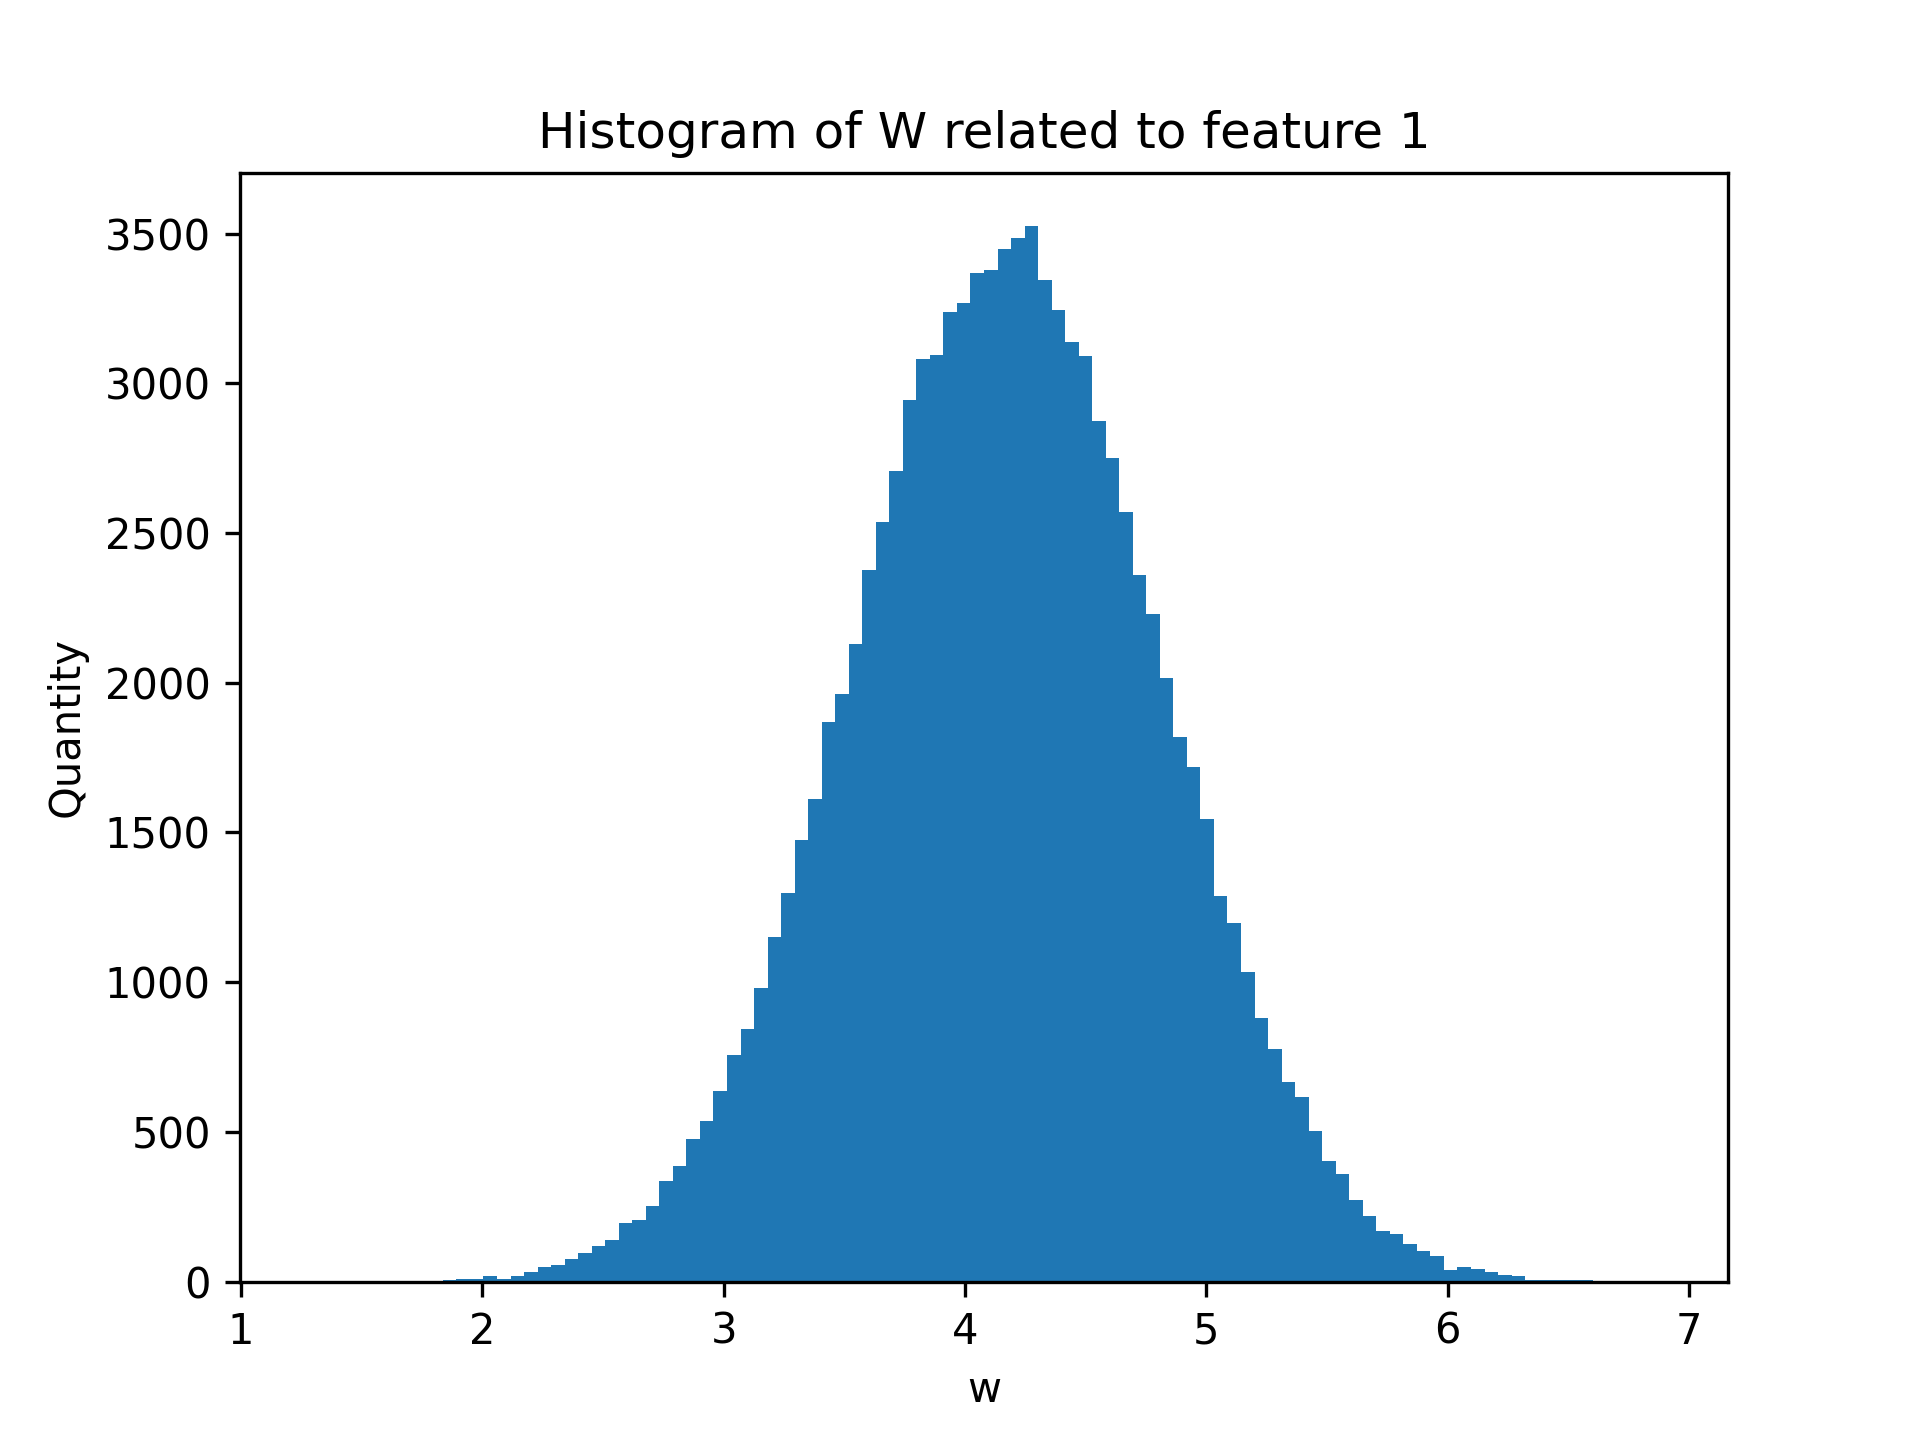
\includegraphics[width=\linewidth]{hist_feat0_349000000_sample_100000.png}
    \caption{$\alpha = 34.9$; $S = 100000$.}
  \end{subfigure}
  \caption{Histogram of W for feature 1 with differents learning rates ($\alpha$) and sample sizes ($S$) for Monte Carlo approximation.}
  \label{fig:hist_feat0}
\end{figure}


% Histogram - Feature 2
\begin{figure}
  \centering
  \begin{subfigure}[t]{0.24\textwidth}
    \centering
    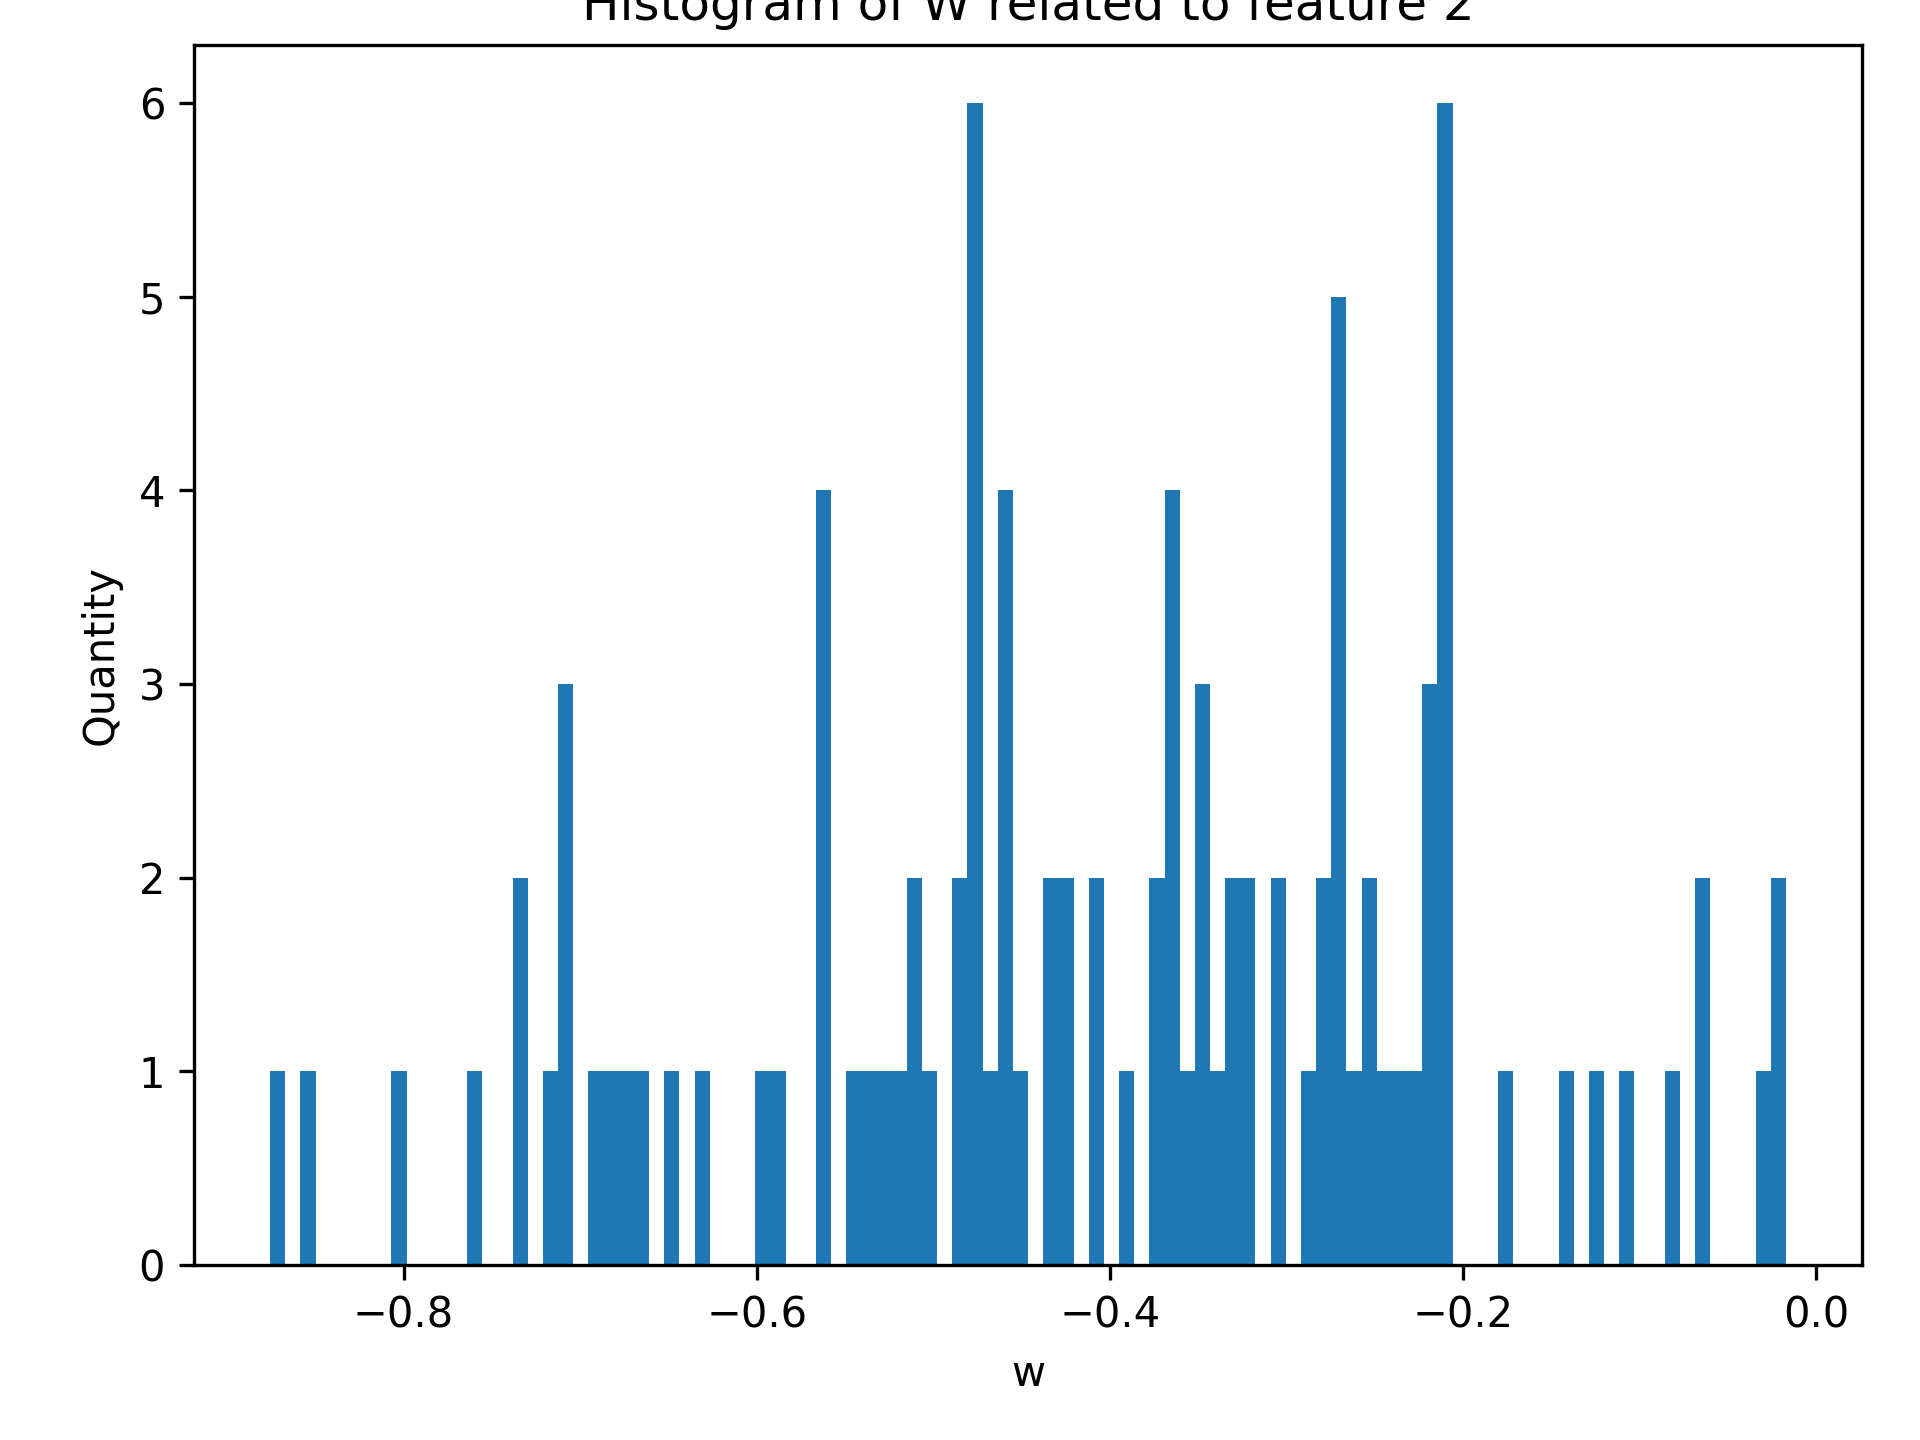
\includegraphics[width=\linewidth]{hist_feat1_1_sample_100.png}
    \caption{$\alpha = 1e-7$; $S = 100$.}
  \end{subfigure}
  \hfill
  \begin{subfigure}[t]{0.24\textwidth}
    \centering
    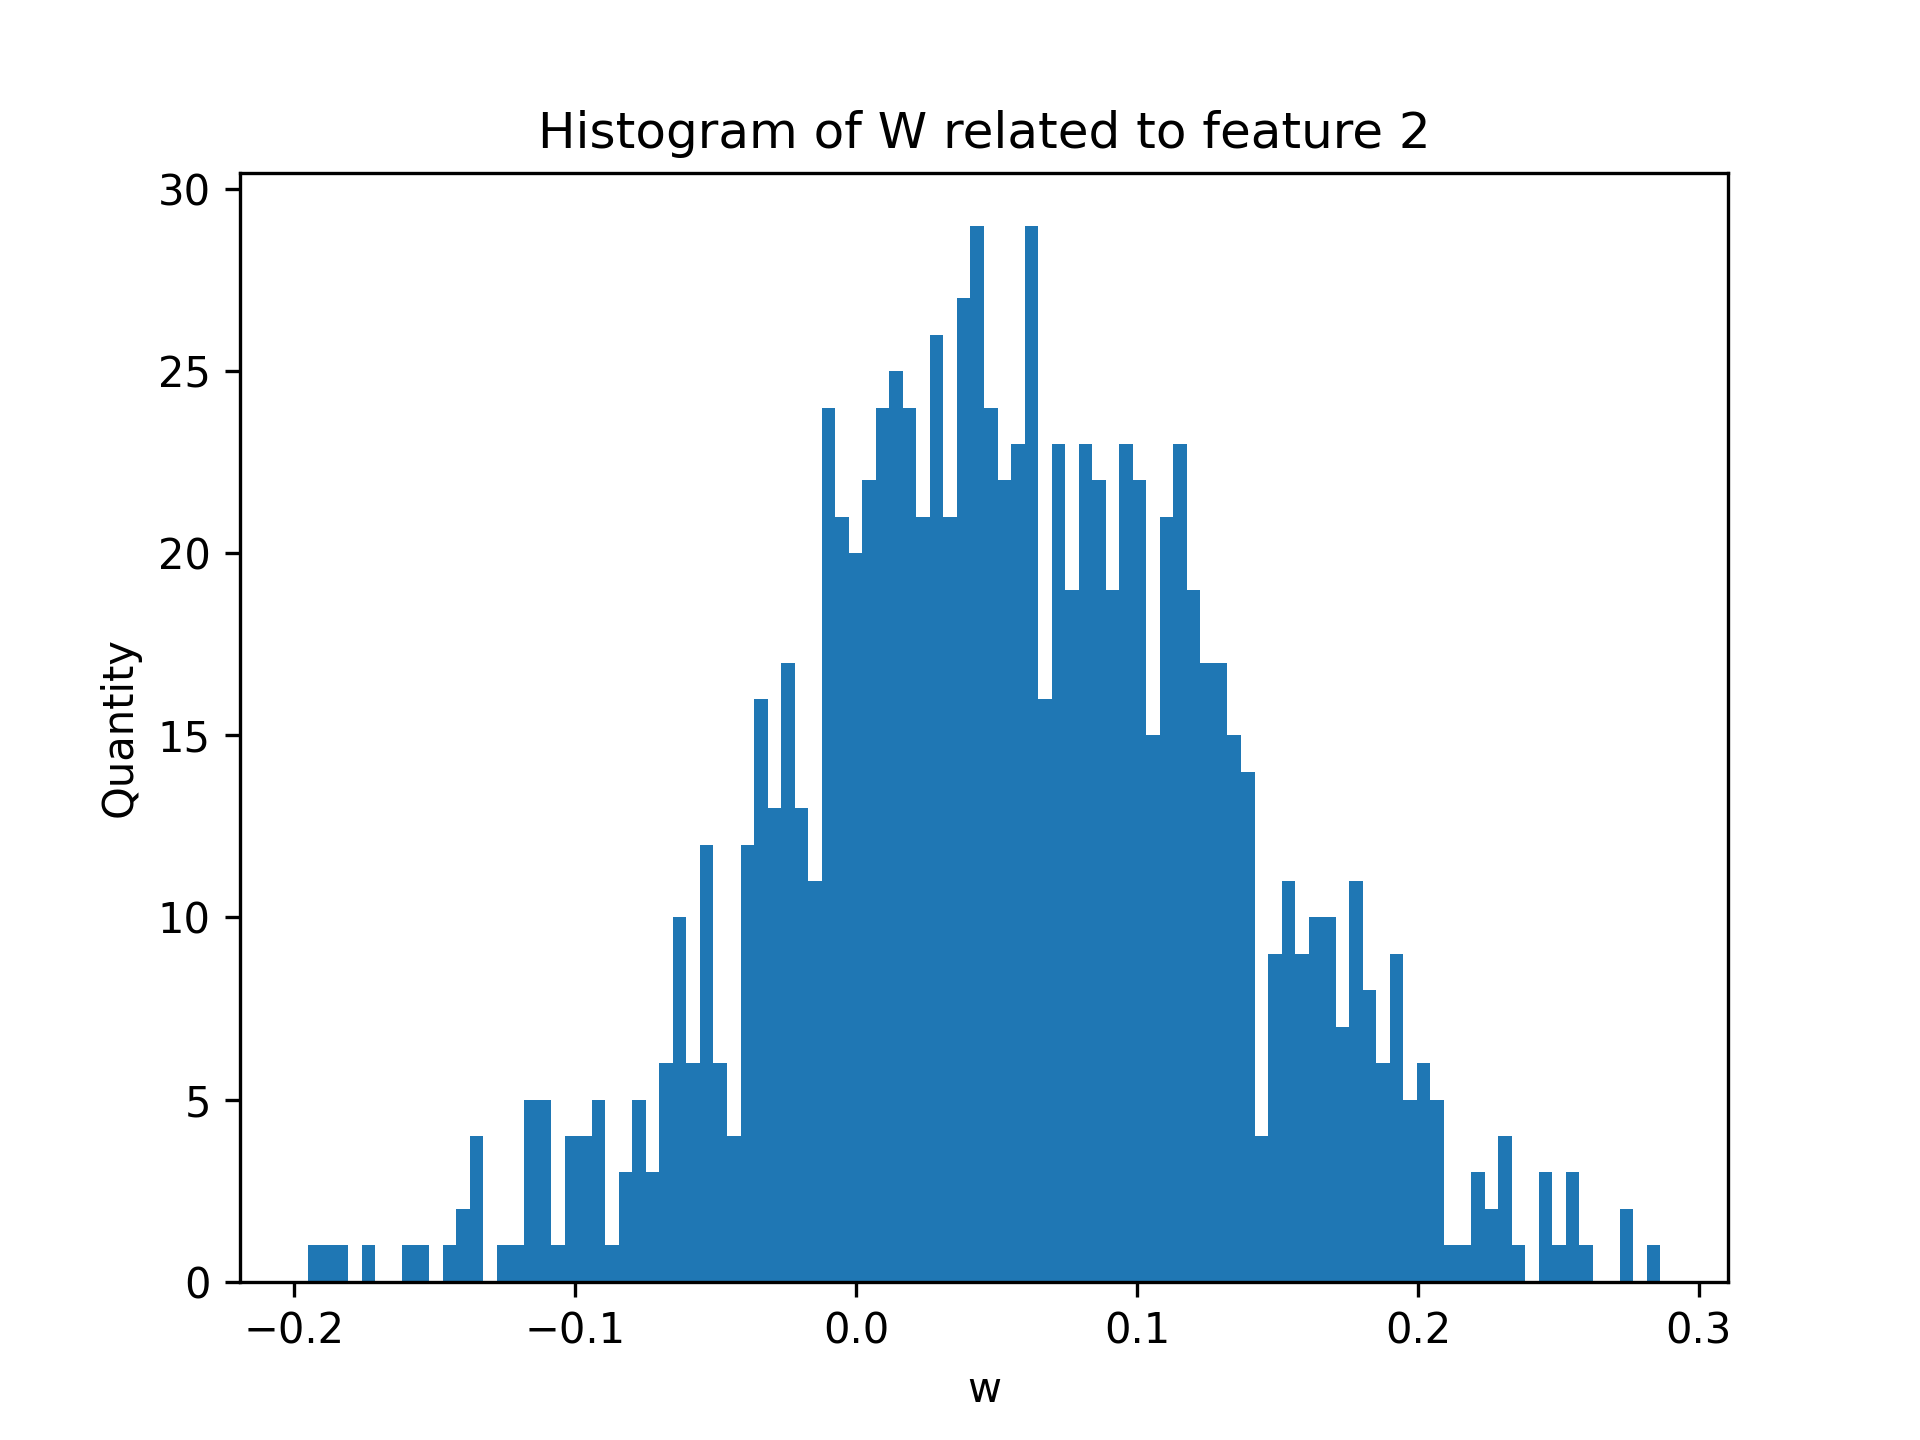
\includegraphics[width=\linewidth]{hist_feat1_1_sample_1000.png}
    \caption{$\alpha = 1e-7$; $S = 1000$.}
  \end{subfigure}
  \hfill
  \begin{subfigure}[t]{0.24\textwidth}
    \centering
    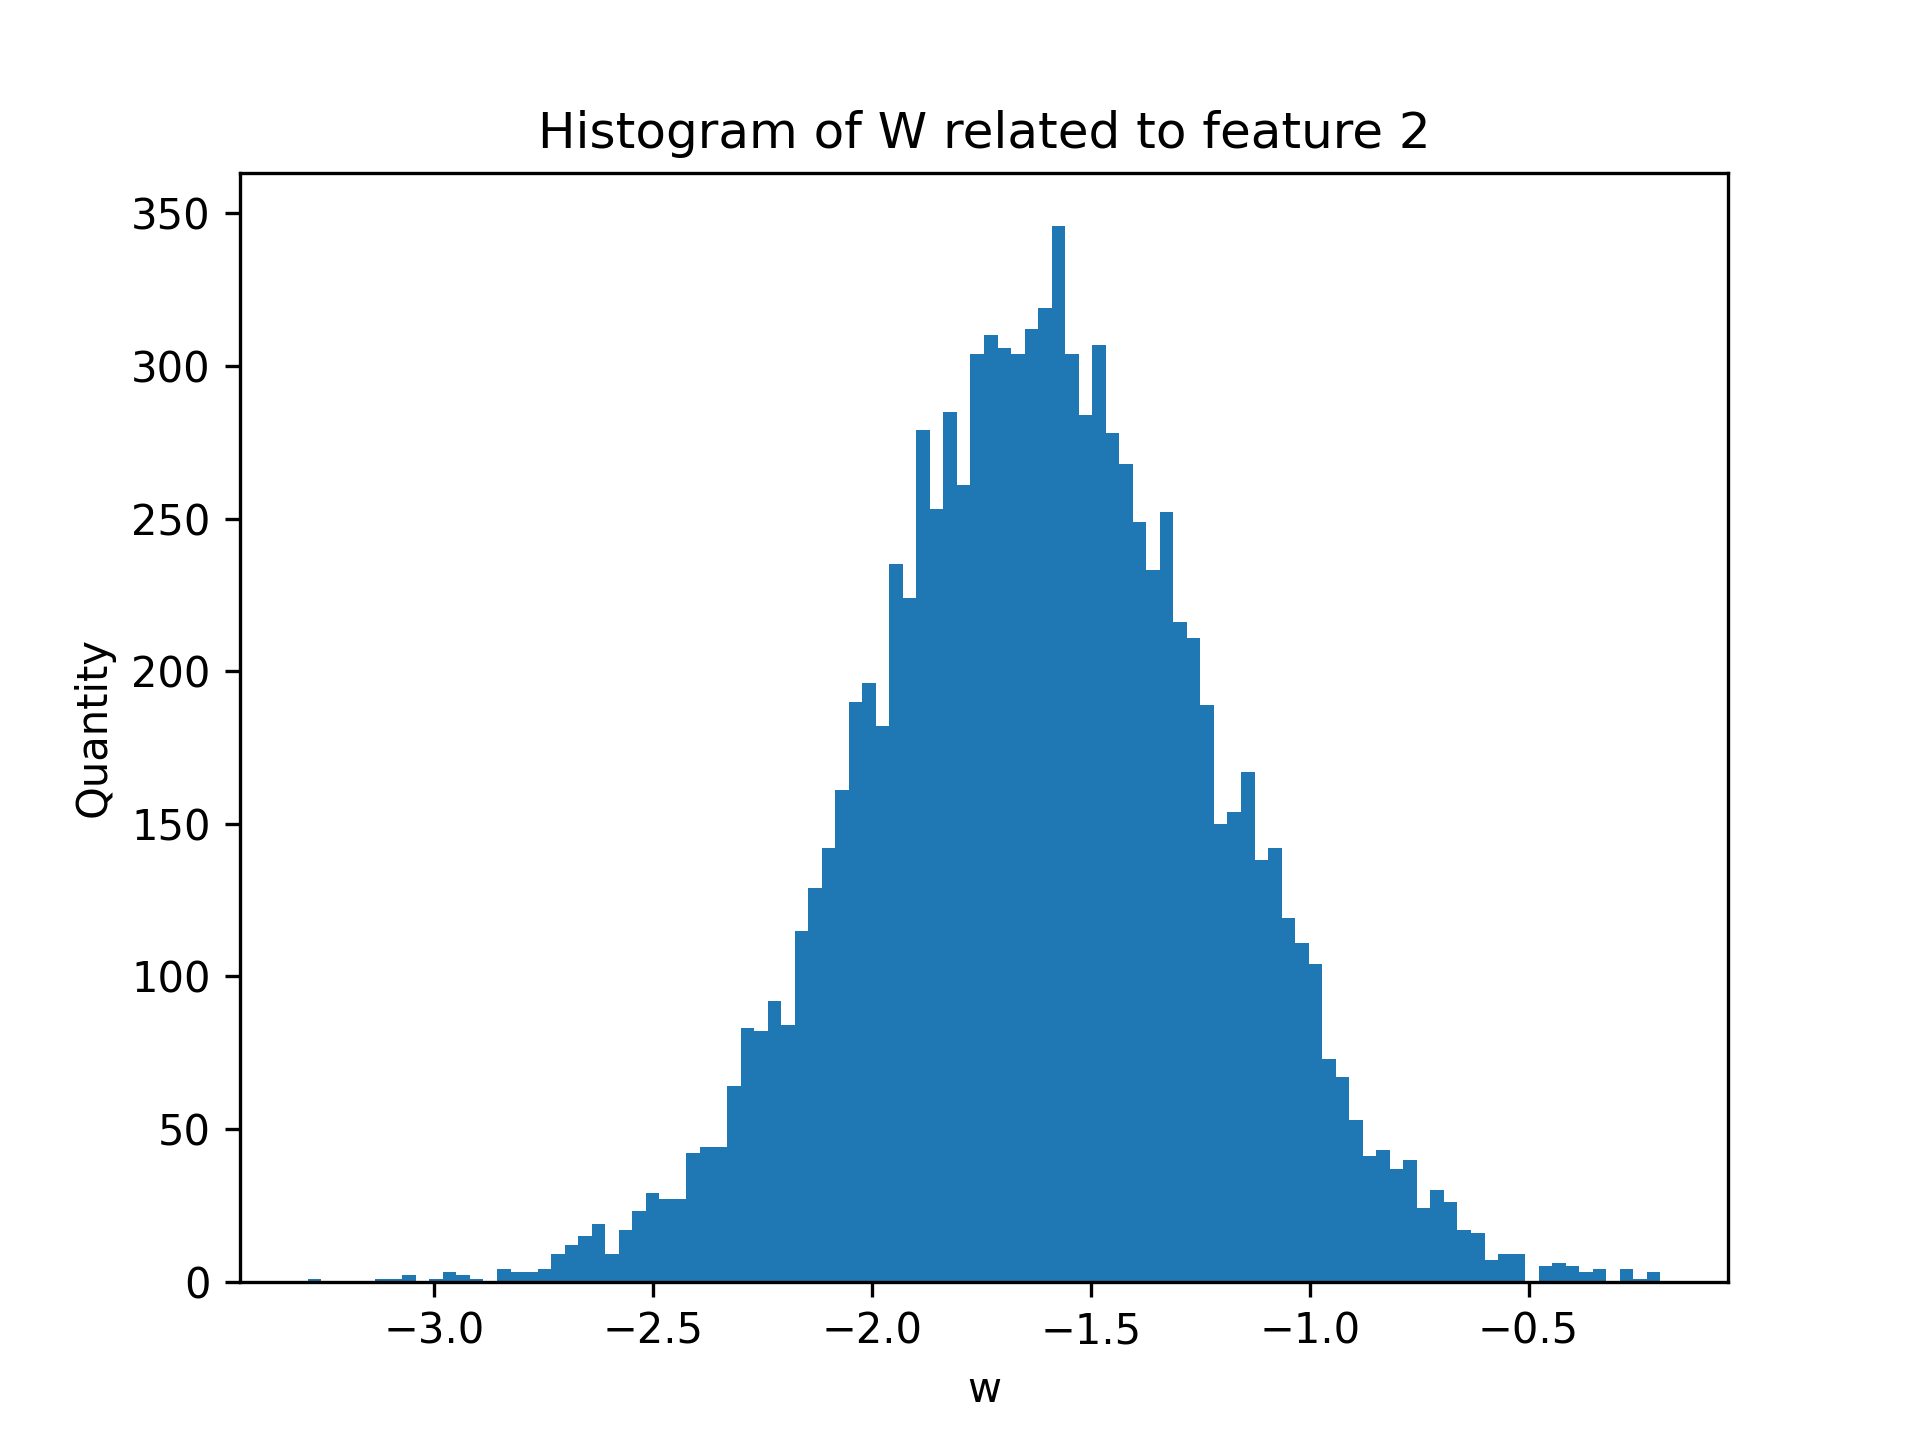
\includegraphics[width=\linewidth]{hist_feat1_1_sample_10000.png}
    % \caption{Learning rate 0.001 and 10000 samples.}
    \caption{$\alpha = 1e-7$; $S = 10000$.}
  \end{subfigure}
  \hfill
  \begin{subfigure}[t]{0.24\textwidth}
    \centering
    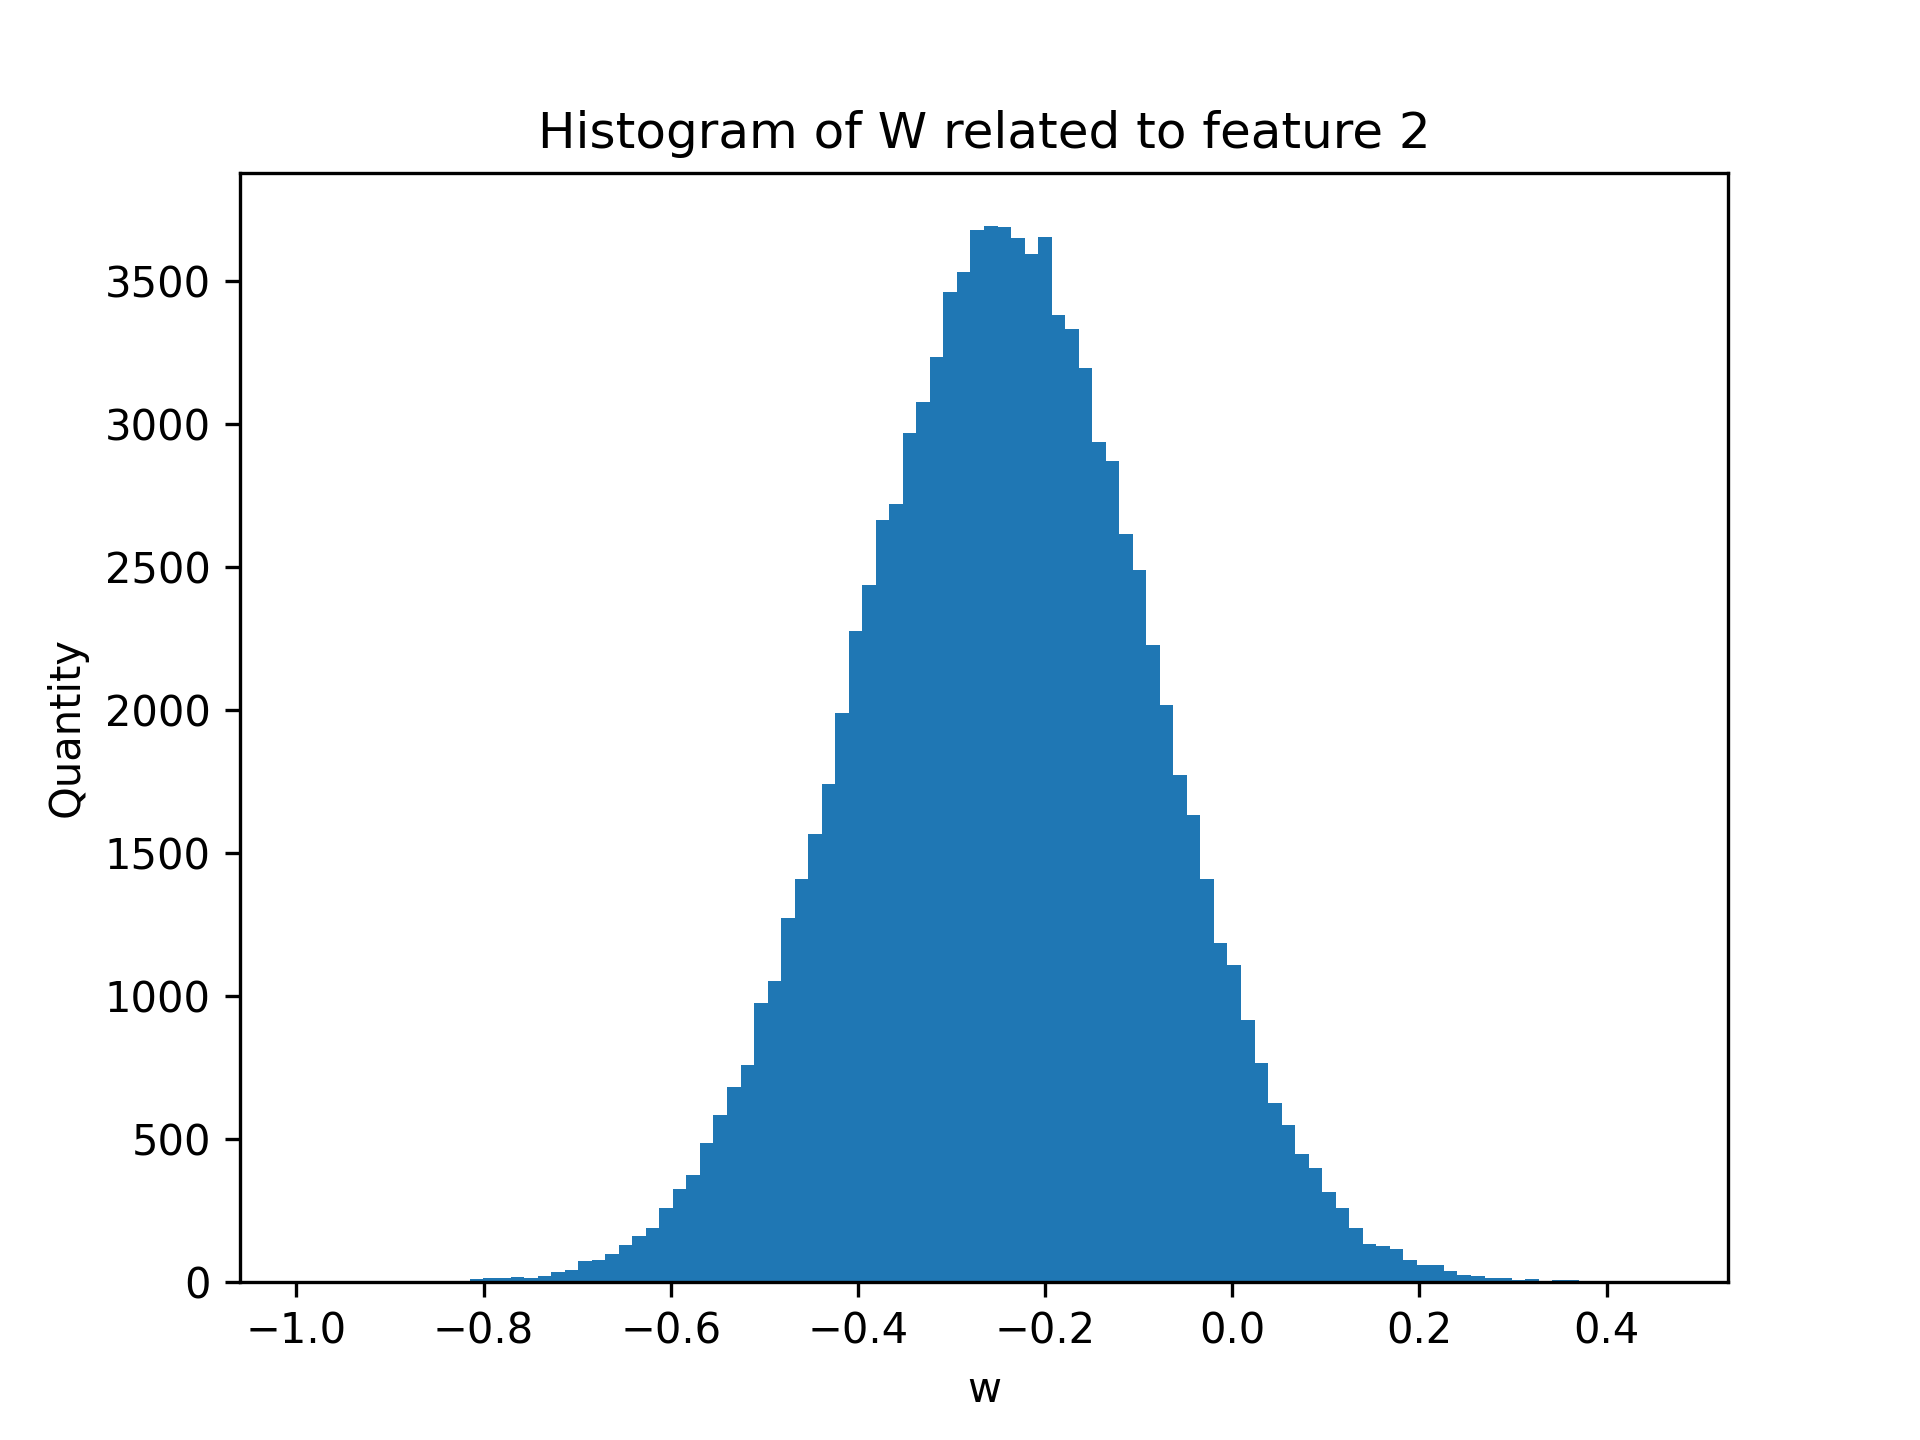
\includegraphics[width=\linewidth]{hist_feat1_1_sample_100000.png}
    \caption{$\alpha = 1e-7$; $S = 100000$.}
  \end{subfigure}
  % \hfill
  \begin{subfigure}[t]{0.24\textwidth}
    \centering
    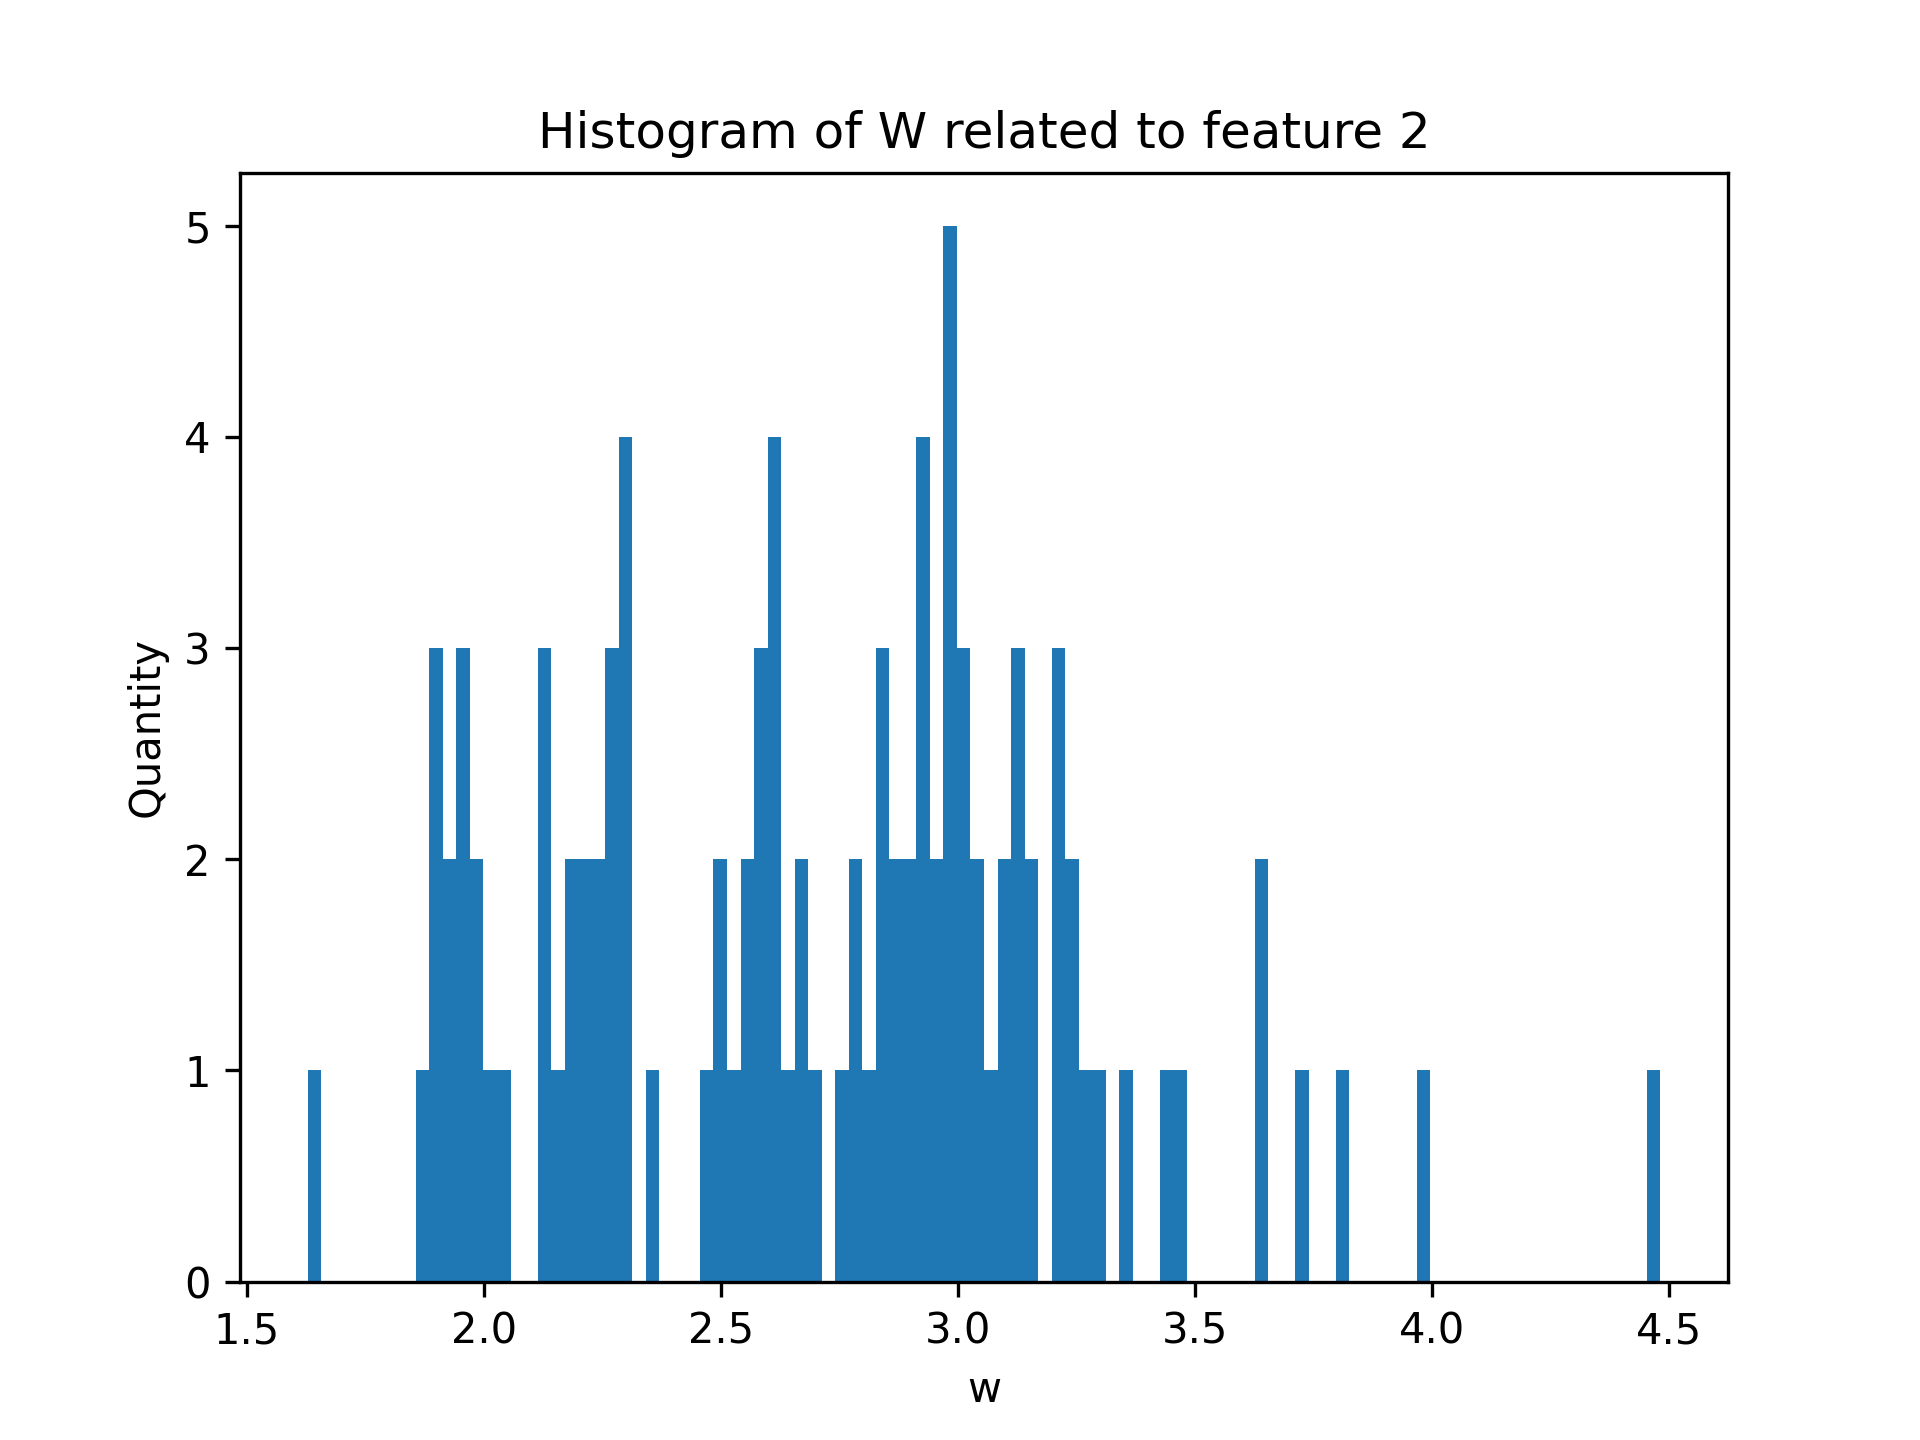
\includegraphics[width=\linewidth]{hist_feat1_10000_sample_100.png}
    \caption{$\alpha = 1e-3$; $S = 100$.}
  \end{subfigure}
  \hfill
  \begin{subfigure}[t]{0.24\textwidth}
    \centering
    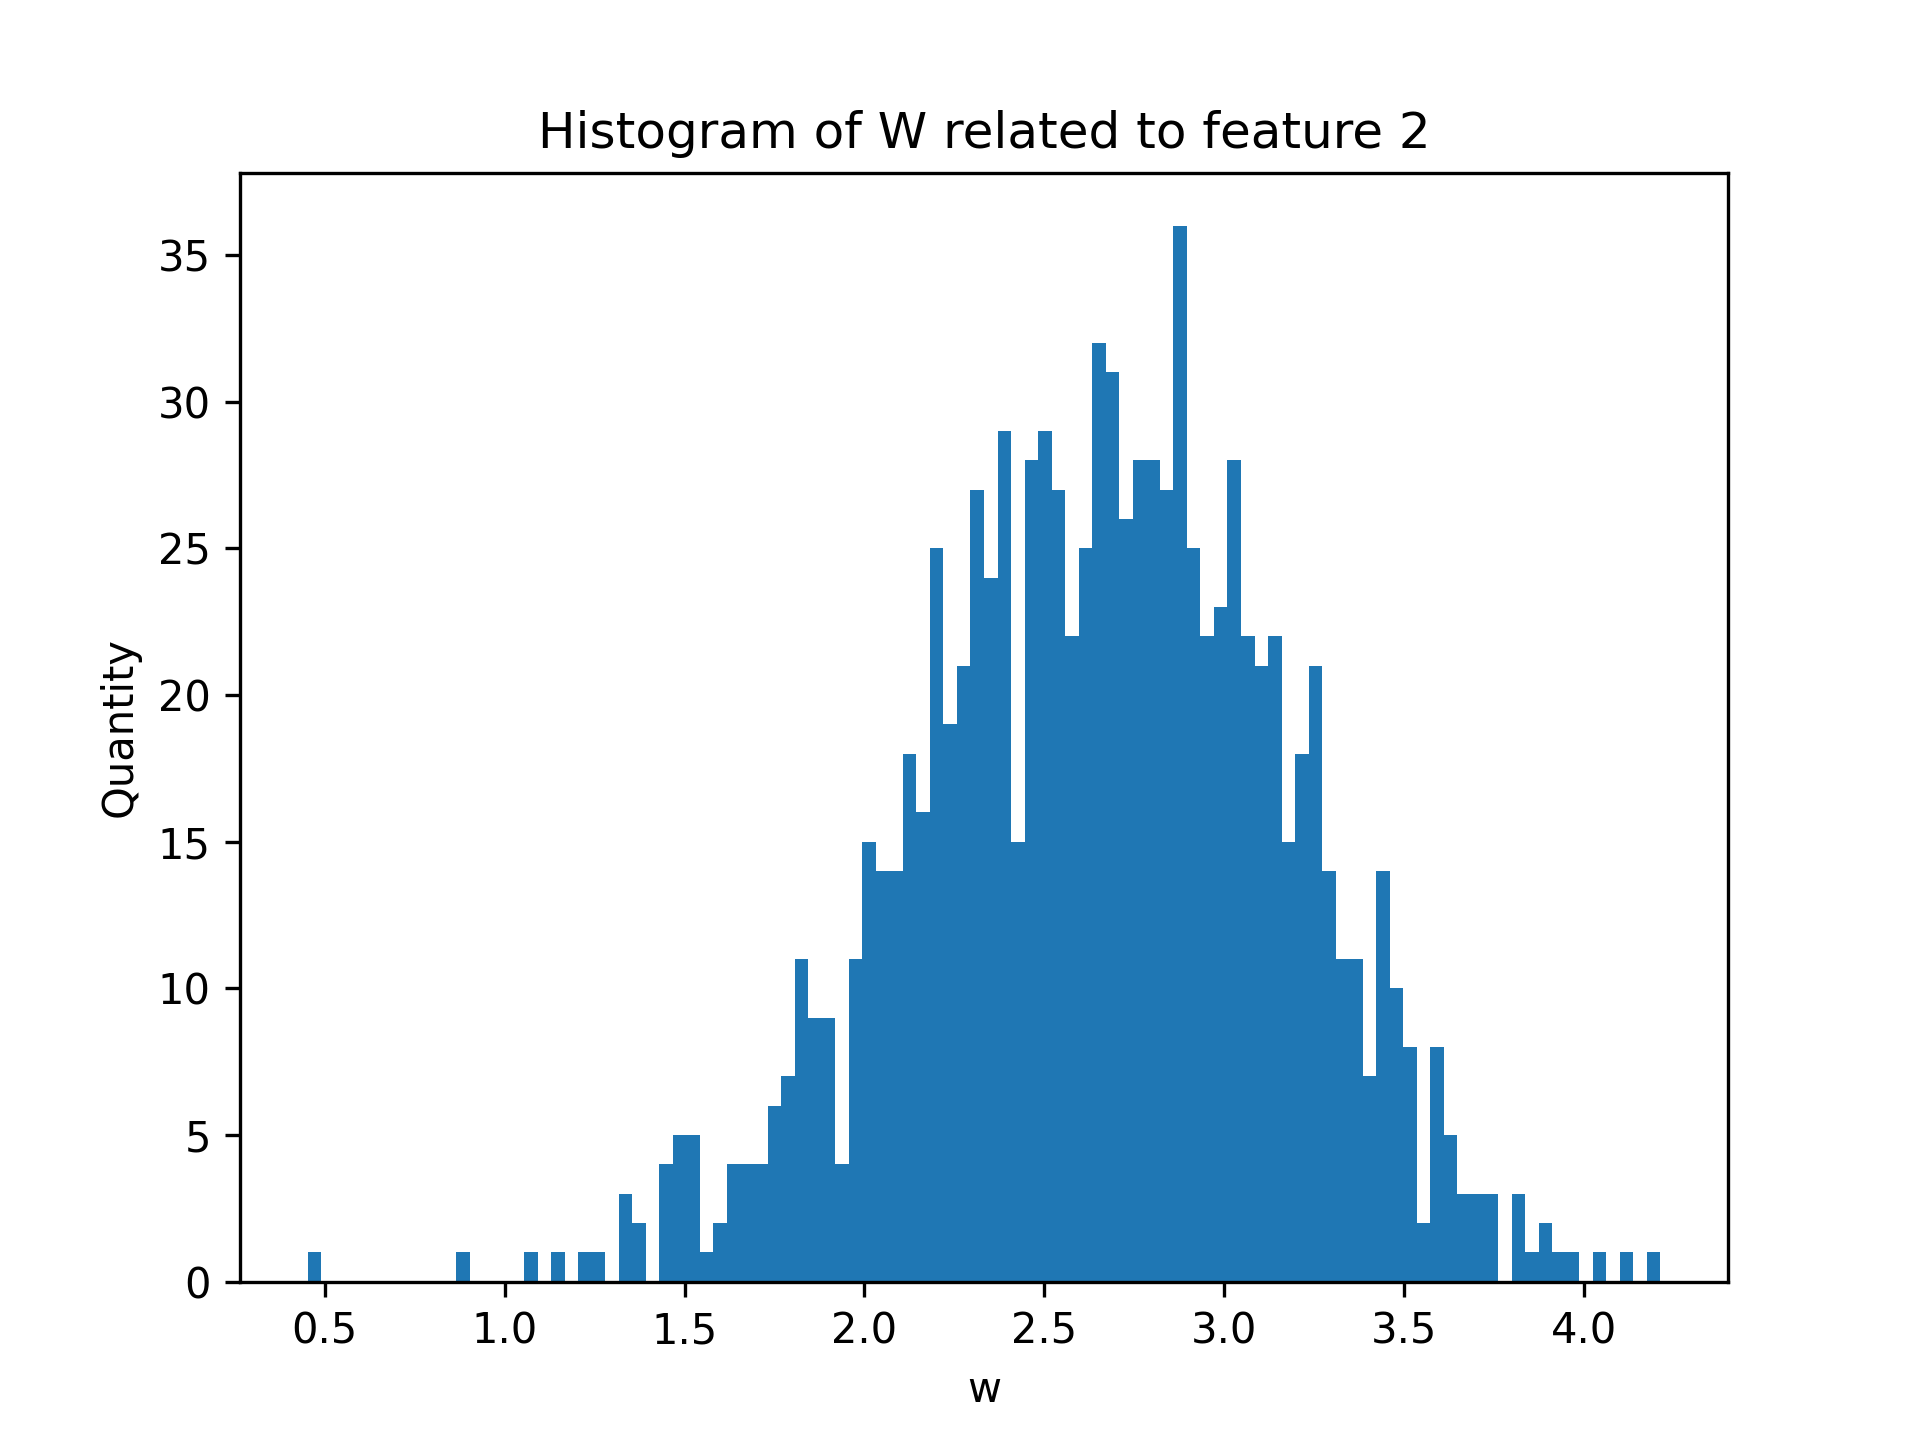
\includegraphics[width=\linewidth]{hist_feat1_10000_sample_1000.png}
    \caption{$\alpha = 1e-3$; $S = 1000$.}
  \end{subfigure}
  \hfill
  \begin{subfigure}[t]{0.24\textwidth}
    \centering
    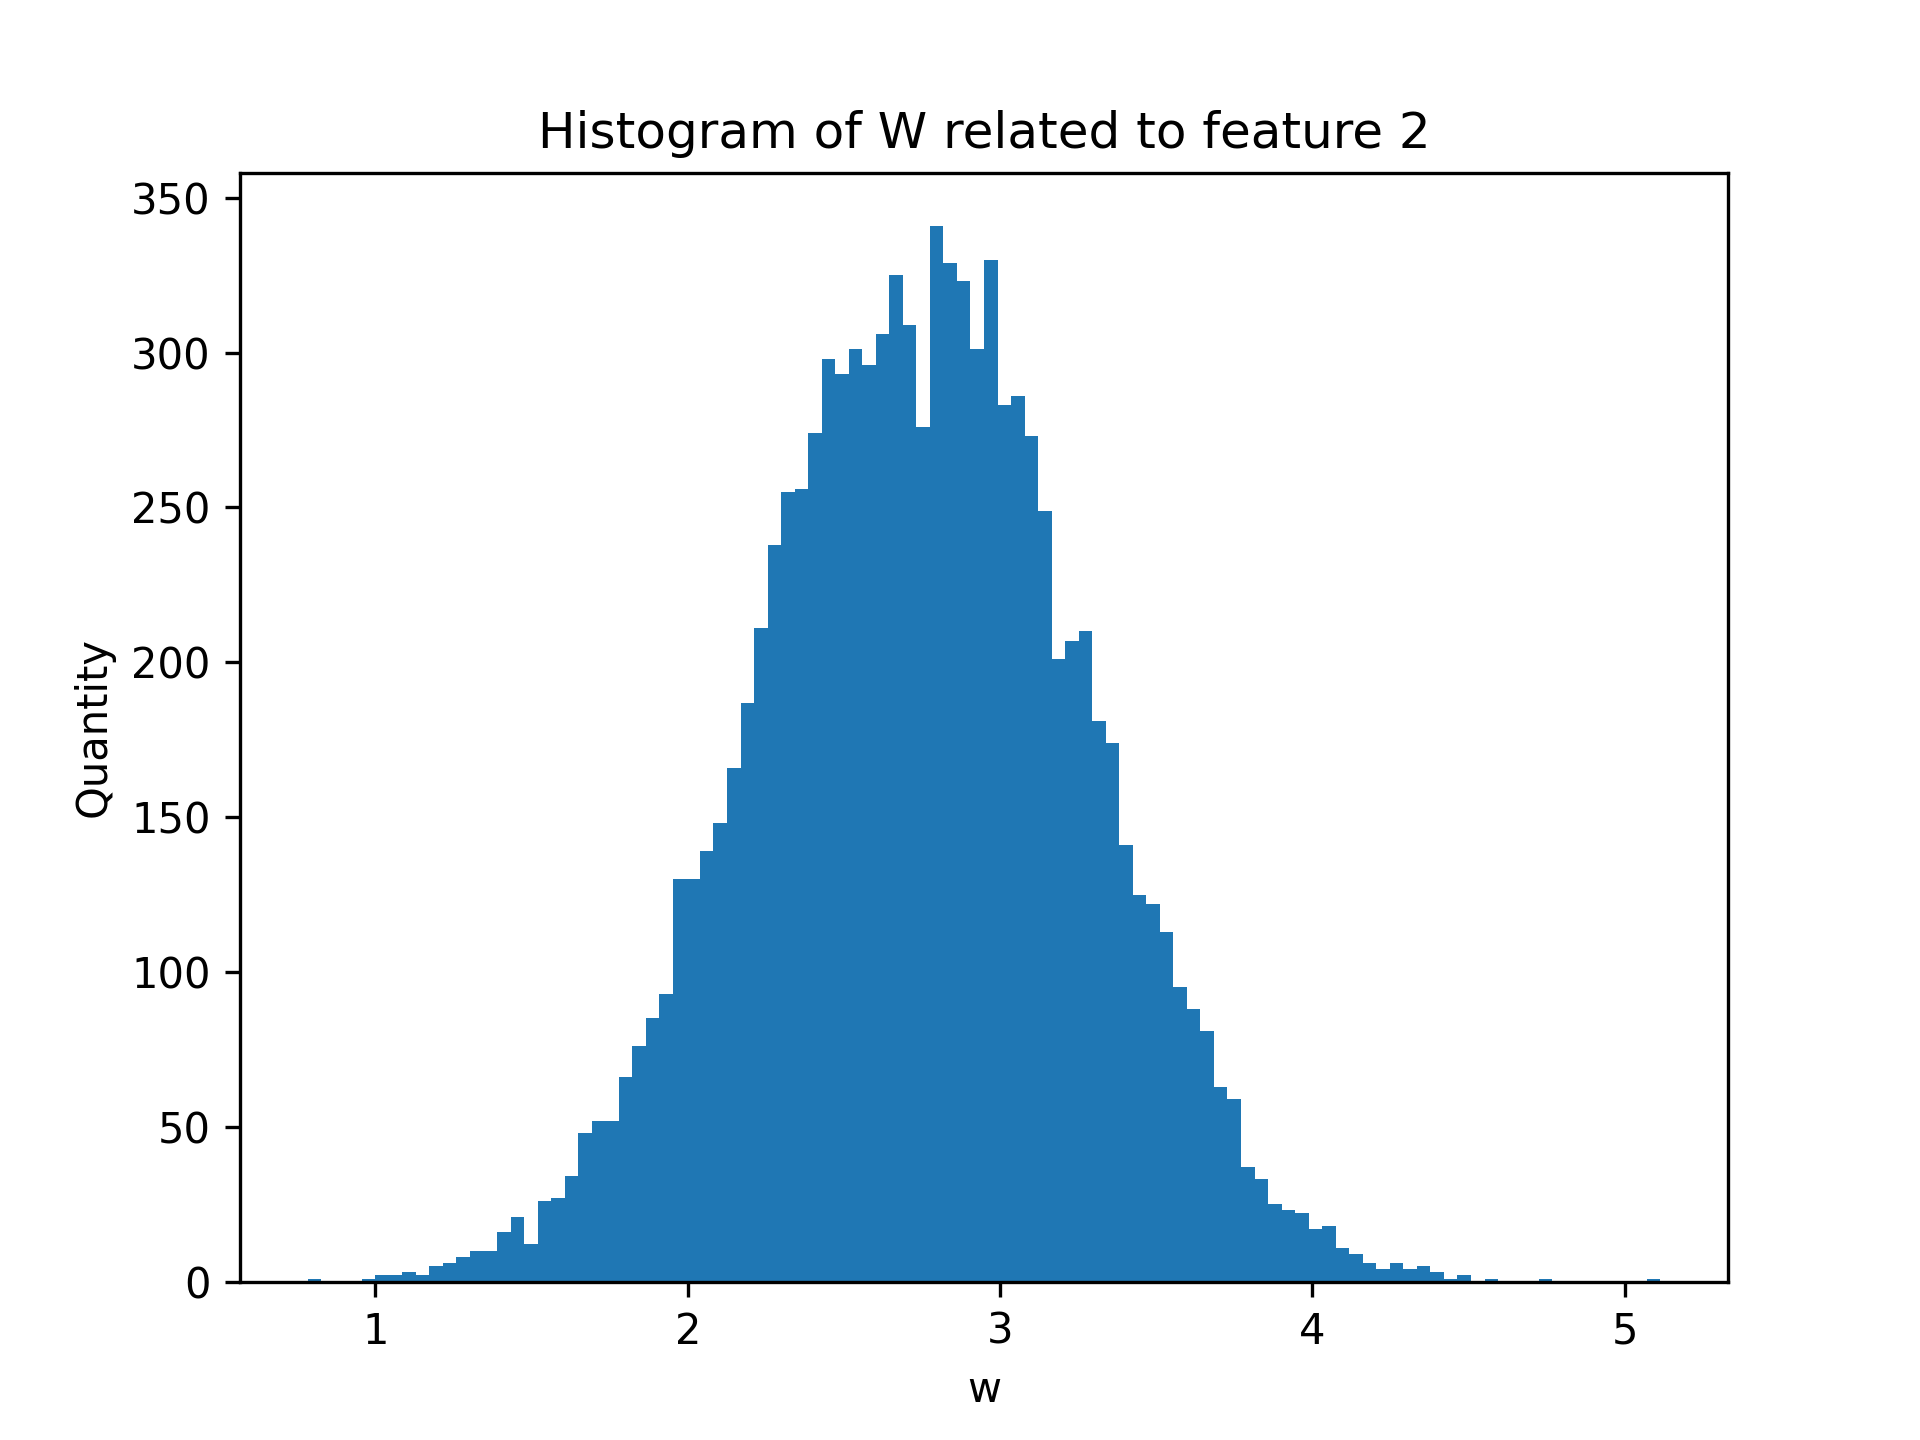
\includegraphics[width=\linewidth]{hist_feat1_10000_sample_10000.png}
    \caption{$\alpha = 1e-3$; $S = 10000$.}
  \end{subfigure}
  \hfill
  \begin{subfigure}[t]{0.24\textwidth}
    \centering
    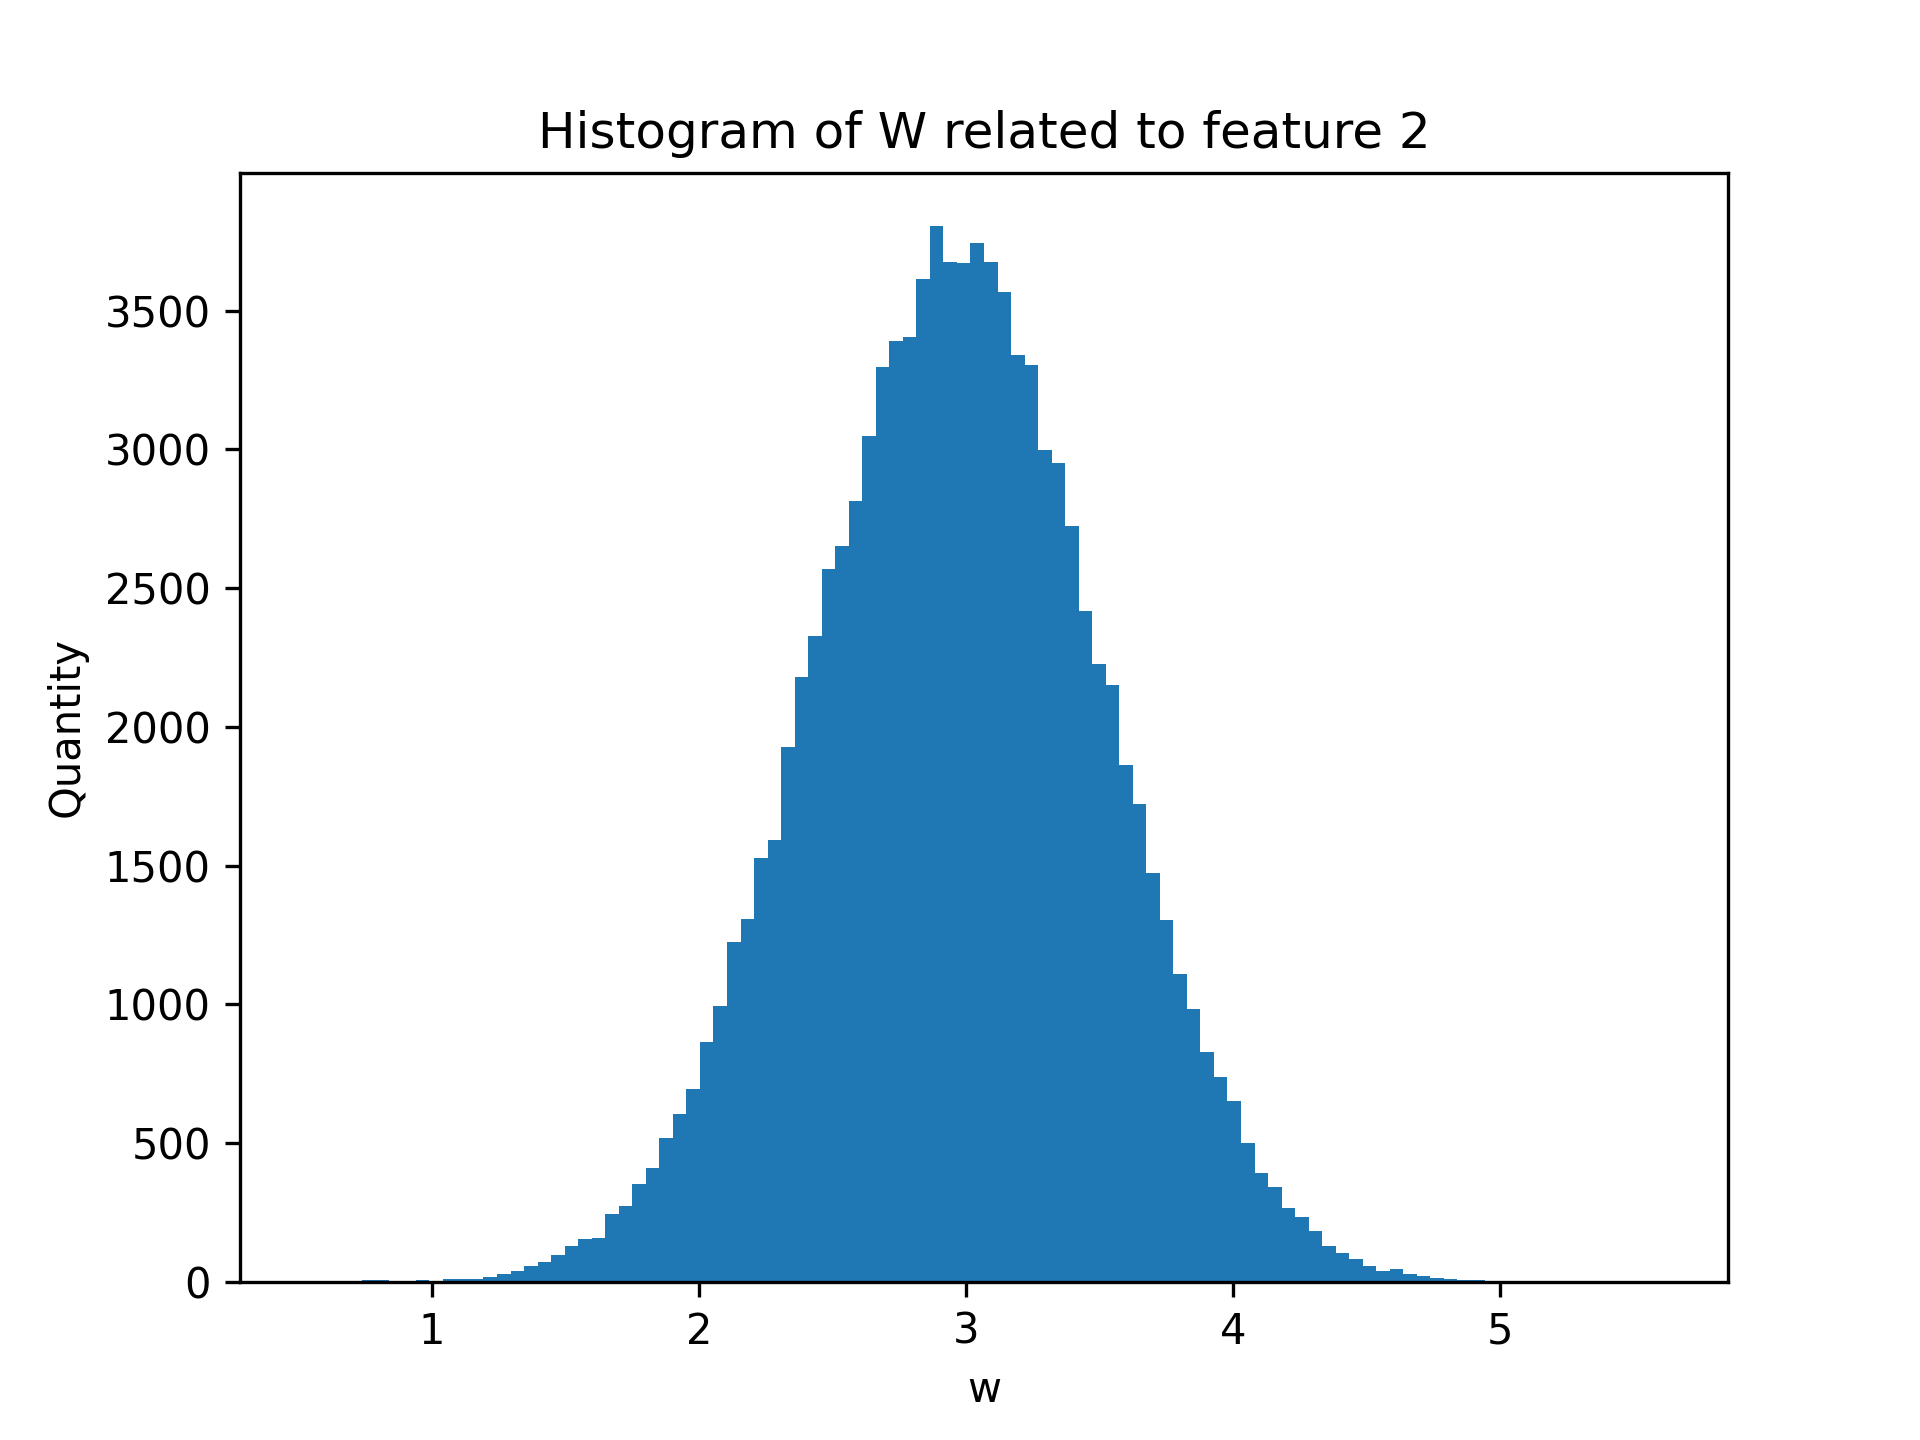
\includegraphics[width=\linewidth]{hist_feat1_10000_sample_100000.png}
    \caption{$\alpha = 1e-3$; $S = 100000$.}
  \end{subfigure}
  % \hfill
  \begin{subfigure}[t]{0.24\textwidth}
    \centering
    \includegraphics[width=\linewidth]{hist_feat1_349000000_sample_100.png}
    \caption{$\alpha = 34.9$; $S = 100$.}
  \end{subfigure}
  \hfill
  \begin{subfigure}[t]{0.24\textwidth}
    \centering
    \includegraphics[width=\linewidth]{hist_feat1_349000000_sample_1000.png}
    \caption{$\alpha = 34.9$; $S = 1000$.}
  \end{subfigure}
  \hfill
  \begin{subfigure}[t]{0.24\textwidth}
    \centering
    \includegraphics[width=\linewidth]{hist_feat1_349000000_sample_10000.png}
    \caption{$\alpha = 34.9$; $S = 10000$.}
  \end{subfigure}
  \hfill
  \begin{subfigure}[t]{0.24\textwidth}
    \centering
    \includegraphics[width=\linewidth]{hist_feat1_349000000_sample_100000.png}
    \caption{$\alpha = 34.9$; $S = 100000$.}
  \end{subfigure}
  \caption{Histogram of W for feature 2 with differents learning rates ($\alpha$) and sample sizes ($S$) for Monte Carlo approximation.}
  \label{fig:hist_feat1}
\end{figure}


\begin{table}[h]
  \centering
  \caption{Performance evaluation of discriminative model for learning rate $1e-07$ and 100 samples} \label{tab:4}
  \begin{tabular}{ccccccc}
  \cline{2-7}
  & \multicolumn{6}{c}{\textbf{Dataset C (\%)}} \\ \cline{2-7}
  & \multicolumn{3}{c}{\textbf{Training set}} & \multicolumn{3}{c}{\textbf{Testing set}} \\ \hline
  \textbf{Classes} & \textbf{Accuracy} & \textbf{Precision} & \textbf{Recall} & \textbf{Accuracy} & \textbf{Precision} & \textbf{Recall} \\ \hline
  \textbf{0} & \multirow{2}{*}{42.0} & 45.65 & 84.0 & \multirow{2}{*}{48.0} & 48.97 & 96.0 \\ \cline{1-1} \cline{3-4} \cline{6-7} 
  \textbf{1} &  & 0.0 & 0.0 &  & 0.0 & 0.0 \\ \hline
  \end{tabular}
  \end{table}
  
  \begin{table}[h]
  \centering
  \caption{Performance evaluation of discriminative model for learning rate 1e-07 and 1000 samples} \label{tab:5}
  \begin{tabular}{ccccccc}
  \cline{2-7}
  & \multicolumn{6}{c}{\textbf{Dataset C (\%)}} \\ \cline{2-7}
  & \multicolumn{3}{c}{\textbf{Training set}} & \multicolumn{3}{c}{\textbf{Testing set}} \\ \hline
  \textbf{Classes} & \textbf{Accuracy} & \textbf{Precision} & \textbf{Recall} & \textbf{Accuracy} & \textbf{Precision} & \textbf{Recall} \\ \hline
  \textbf{0} & \multirow{2}{*}{50.0} & 50.0 & 100.0 & \multirow{2}{*}{50.0} & 50.0 & 100.0 \\ \cline{1-1} \cline{3-4} \cline{6-7} 
  \textbf{1} &  & 0 & 0.0 &  & 0 & 0.0 \\ \hline
  \end{tabular}
  \end{table}
  
  \begin{table}[h]
  \centering
  \caption{Performance evaluation of discriminative model for learning rate 1e-07 and 10000 samples} \label{tab:6}
  \begin{tabular}{ccccccc}
  \cline{2-7}
  & \multicolumn{6}{c}{\textbf{Dataset C (\%)}} \\ \cline{2-7}
  & \multicolumn{3}{c}{\textbf{Training set}} & \multicolumn{3}{c}{\textbf{Testing set}} \\ \hline
  \textbf{Classes} & \textbf{Accuracy} & \textbf{Precision} & \textbf{Recall} & \textbf{Accuracy} & \textbf{Precision} & \textbf{Recall} \\ \hline
  \textbf{0} & \multirow{2}{*}{10.0} & 14.28 & 16.0 & \multirow{2}{*}{14} & 20.0 & 24.0 \\ \cline{1-1} \cline{3-4} \cline{6-7} 
  \textbf{1} &  & 4.54 & 4.0 &  & 5.0 & 4.0 \\ \hline
  \end{tabular}
  \end{table}
  
  \begin{table}[h]
  \centering
  \caption{Performance evaluation of discriminative model for learning rate 1e-07 and 100000 samples} \label{tab:7}
  \begin{tabular}{ccccccc}
  \cline{2-7}
  & \multicolumn{6}{c}{\textbf{Dataset C (\%)}} \\ \cline{2-7}
  & \multicolumn{3}{c}{\textbf{Training set}} & \multicolumn{3}{c}{\textbf{Testing set}} \\ \hline
  \textbf{Classes} & \textbf{Accuracy} & \textbf{Precision} & \textbf{Recall} & \textbf{Accuracy} & \textbf{Precision} & \textbf{Recall} \\ \hline
  \textbf{0} & \multirow{2}{*}{42.0} & 45.45 & 80.0 & \multirow{2}{*}{46.0} & 47.91 & 92.0 \\ \cline{1-1} \cline{3-4} \cline{6-7} 
  \textbf{1} &  & 16.66 & 4.0 &  & 0.0 & 0.0 \\ \hline
  \end{tabular}
  \end{table}
  
  \begin{table}[h]
  \centering
  \caption{Performance evaluation of discriminative model for learning rate 0.001 and 100 samples} \label{tab:8}
  \begin{tabular}{ccccccc}
  \cline{2-7}
  & \multicolumn{6}{c}{\textbf{Dataset C (\%)}} \\ \cline{2-7}
  & \multicolumn{3}{c}{\textbf{Training set}} & \multicolumn{3}{c}{\textbf{Testing set}} \\ \hline
  \textbf{Classes} & \textbf{Accuracy} & \textbf{Precision} & \textbf{Recall} & \textbf{Accuracy} & \textbf{Precision} & \textbf{Recall} \\ \hline
  \textbf{0} & \multirow{2}{*}{100.0} & 100.0 & 100.0 & \multirow{2}{*}{88.0} & 100.0 & 76.0 \\ \cline{1-1} \cline{3-4} \cline{6-7} 
  \textbf{1} &  & 100.0 & 100.0 &  & 80.64 & 100.0 \\ \hline
  \end{tabular}
  \end{table}
  
  \begin{table}[h]
  \centering
  \caption{Performance evaluation of discriminative model for learning rate 0.001 and 1000 samples} \label{tab:9}
  \begin{tabular}{ccccccc}
  \cline{2-7}
  & \multicolumn{6}{c}{\textbf{Dataset C (\%)}} \\ \cline{2-7}
  & \multicolumn{3}{c}{\textbf{Training set}} & \multicolumn{3}{c}{\textbf{Testing set}} \\ \hline
  \textbf{Classes} & \textbf{Accuracy} & \textbf{Precision} & \textbf{Recall} & \textbf{Accuracy} & \textbf{Precision} & \textbf{Recall} \\ \hline
  \textbf{0} & \multirow{2}{*}{100.0} & 100.0 & 100.0 & \multirow{2}{*}{90.0} & 100.0 & 80.0 \\ \cline{1-1} \cline{3-4} \cline{6-7} 
  \textbf{1} &  & 100.0 & 100.0 &  & 83.33 & 100.0 \\ \hline
  \end{tabular}
  \end{table}
  
  \begin{table}[h]
  \centering
  \caption{Performance evaluation of discriminative model for learning rate 0.001 and 10000 samples} \label{tab:10}
  \begin{tabular}{ccccccc}
  \cline{2-7}
  & \multicolumn{6}{c}{\textbf{Dataset C (\%)}} \\ \cline{2-7}
  & \multicolumn{3}{c}{\textbf{Training set}} & \multicolumn{3}{c}{\textbf{Testing set}} \\ \hline
  \textbf{Classes} & \textbf{Accuracy} & \textbf{Precision} & \textbf{Recall} & \textbf{Accuracy} & \textbf{Precision} & \textbf{Recall} \\ \hline
  \textbf{0} & \multirow{2}{*}{100.0} & 100.0 & 100.0 & \multirow{2}{*}{90.0} & 100.0 & 80.0 \\ \cline{1-1} \cline{3-4} \cline{6-7} 
  \textbf{1} &  & 100.0 & 100.0 &  & 83.33 & 100.0 \\ \hline
  \end{tabular}
  \end{table}
  
  \begin{table}[h]
  \centering
  \caption{Performance evaluation of discriminative model for learning rate 0.001 and 100000 samples} \label{tab:11}
  \begin{tabular}{ccccccc}
  \cline{2-7}
  & \multicolumn{6}{c}{\textbf{Dataset C (\%)}} \\ \cline{2-7}
  & \multicolumn{3}{c}{\textbf{Training set}} & \multicolumn{3}{c}{\textbf{Testing set}} \\ \hline
  \textbf{Classes} & \textbf{Accuracy} & \textbf{Precision} & \textbf{Recall} & \textbf{Accuracy} & \textbf{Precision} & \textbf{Recall} \\ \hline
  \textbf{0} & \multirow{2}{*}{100.0} & 100.0 & 100.0 & \multirow{2}{*}{90.0} & 100.0 & 80.0 \\ \cline{1-1} \cline{3-4} \cline{6-7} 
  \textbf{1} &  & 100.0 & 100.0 &  & 83.333 & 100.0 \\ \hline
  \end{tabular}
  \end{table}
  
  \begin{table}[h]
  \centering
  \caption{Performance evaluation of discriminative model for learning rate 34.9 and 100 samples} \label{tab:12}
  \begin{tabular}{ccccccc}
  \cline{2-7}
  & \multicolumn{6}{c}{\textbf{Dataset C (\%)}} \\ \cline{2-7}
  & \multicolumn{3}{c}{\textbf{Training set}} & \multicolumn{3}{c}{\textbf{Testing set}} \\ \hline
  \textbf{Classes} & \textbf{Accuracy} & \textbf{Precision} & \textbf{Recall} & \textbf{Accuracy} & \textbf{Precision} & \textbf{Recall} \\ \hline
  \textbf{0} & \multirow{2}{*}{100.0} & 100.0 & 100.0 & \multirow{2}{*}{92.0} & 100.0 & 84.0 \\ \cline{1-1} \cline{3-4} \cline{6-7} 
  \textbf{1} &  & 100.0 & 100.0 &  & 86.20 & 100.0 \\ \hline
  \end{tabular}
  \end{table}
  
  \begin{table}[h]
  \centering
  \caption{Performance evaluation of discriminative model for learning rate 34.9 and 1000 samples} \label{tab:13}
  \begin{tabular}{ccccccc}
  \cline{2-7}
  & \multicolumn{6}{c}{\textbf{Dataset C (\%)}} \\ \cline{2-7}
  & \multicolumn{3}{c}{\textbf{Training set}} & \multicolumn{3}{c}{\textbf{Testing set}} \\ \hline
  \textbf{Classes} & \textbf{Accuracy} & \textbf{Precision} & \textbf{Recall} & \textbf{Accuracy} & \textbf{Precision} & \textbf{Recall} \\ \hline
  \textbf{0} & \multirow{2}{*}{100.0} & 100.0 & 100.0 & \multirow{2}{*}{92.0} & 100.0 & 84.0 \\ \cline{1-1} \cline{3-4} \cline{6-7} 
  \textbf{1} &  & 100.0 & 100.0 &  & 86.20 & 100.0 \\ \hline
  \end{tabular}
  \end{table}
  
  \begin{table}[h]
  \centering
  \caption{Performance evaluation of discriminative model for learning rate 34.9 and 10000 samples} \label{tab:14}
  \begin{tabular}{ccccccc}
  \cline{2-7}
  & \multicolumn{6}{c}{\textbf{Dataset C (\%)}} \\ \cline{2-7}
  & \multicolumn{3}{c}{\textbf{Training set}} & \multicolumn{3}{c}{\textbf{Testing set}} \\ \hline
  \textbf{Classes} & \textbf{Accuracy} & \textbf{Precision} & \textbf{Recall} & \textbf{Accuracy} & \textbf{Precision} & \textbf{Recall} \\ \hline
  \textbf{0} & \multirow{2}{*}{100.0} & 100.0 & 100.0 & \multirow{2}{*}{92.0} & 100.0 & 84.0 \\ \cline{1-1} \cline{3-4} \cline{6-7} 
  \textbf{1} &  & 100.0 & 100.0 &  & 86.20 & 100.0 \\ \hline
  \end{tabular}
  \end{table}
  
  \begin{table}[h]
  \centering
  \caption{Performance evaluation of discriminative model for learning rate 34.9 and 100000 samples} \label{tab:15}
  \begin{tabular}{ccccccc}
  \cline{2-7}
  & \multicolumn{6}{c}{\textbf{Dataset C (\%)}} \\ \cline{2-7}
  & \multicolumn{3}{c}{\textbf{Training set}} & \multicolumn{3}{c}{\textbf{Testing set}} \\ \hline
  \textbf{Classes} & \textbf{Accuracy} & \textbf{Precision} & \textbf{Recall} & \textbf{Accuracy} & \textbf{Precision} & \textbf{Recall} \\ \hline
  \textbf{0} & \multirow{2}{*}{100.0} & 100.0 & 100.0 & \multirow{2}{*}{90.0} & 100.0 & 80.0 \\ \cline{1-1} \cline{3-4} \cline{6-7} 
  \textbf{1} &  & 100.0 & 100.0 &  & 83.33 & 100.0 \\ \hline
  \end{tabular}
  \end{table}

\section{Conclusion}

In this project, we implemented two types of machine learning algorithms to predict classes: generative and discriminative. In the probabilistic generative model, we fitted three linear decision boundary for three classes in each dataset. We achieved an accuracy of 73\% and 95\% in the test set of dataset A and B, respectively. In the discriminative model, we applied a gradient descent algorithm to maximize likelihood function of a logistic regression, and used Monte Carlo sampling in the prediction step, which for good choices of learning rate, achieved a reasonable performance, with high values of accuracy, precision and recall, and for a bad choice of learning rate, those metrics achieved bad results, what was expected. In addition, both models yield linear decision boundaries to classify data between classes. Further, the training procedures are different; the generative approach maximize the joint log-likelihood and the discriminative maximize the conditional log-likelihood. However, logistic regression should performe better than the probabilistic generative model, when Gaussian assumptions are not applicable, e. g., with outlier data.

\printbibliography

\end{document}